% TMLR submission: HyperKKL design study. Anonymous submission mode (no [accepted] option).
% Build: cd paper && pdflatex main && bibtex main && pdflatex main && pdflatex main
% Every number in the text is a macro from generated/numbers.tex or a generated table/figure
% (paper/generated/, regenerated by `python -m analysis.paper_results`); nothing is typed by hand.
\documentclass{article}
\usepackage{style/tmlr}            % official TMLR style (github.com/JmlrOrg/tmlr-style-file)
\usepackage[utf8]{inputenc}
\usepackage{amsmath,amssymb,amsthm,mathtools,bm}
\usepackage{booktabs,longtable,array,multirow}
\usepackage{graphicx}
\usepackage{enumitem}
\usepackage{xcolor}
\usepackage{tikz}
\usetikzlibrary{arrows.meta,positioning,calc}
\usepackage{microtype}
\usepackage[font=small,skip=4pt]{caption}
\usepackage{placeins}
% float pages ([p]) start at the top of the page instead of being vertically centred
\makeatletter\setlength{\@fptop}{0pt}\setlength{\@fpsep}{12pt plus 2fil}\setlength{\@fpbot}{0pt plus 1fil}\makeatother
\usepackage[colorlinks=true,linkcolor=blue!50!black,citecolor=blue!50!black,urlcolor=blue!50!black]{hyperref}
\usepackage{url}
\graphicspath{{generated/}{../experiments/real/figures/}}

% ---- theorem environments: identical to theory/main.tex so the theory files \input below compile
\newtheorem{theorem}{Theorem}
\newtheorem{lemma}[theorem]{Lemma}
\newtheorem{proposition}[theorem]{Proposition}
\newtheorem{corollary}[theorem]{Corollary}
\newtheorem{conjecture}[theorem]{Conjecture}
\theoremstyle{definition}
\newtheorem{assumption}{Assumption}
\newtheorem{definition}[theorem]{Definition}
\newtheorem{remark}[theorem]{Remark}
\newtheorem{example}[theorem]{Example}

% ---- numbers produced by the mechanical results layer (analysis/paper_results.py)
% generated by analysis/paper_results.py -- every number quoted in the text. Do not edit.
% generated 2026-10-26 17:43

\providecommand{\ConeConcatBeatsAllId}{}\renewcommand{\ConeConcatBeatsAllId}{0/5}
\providecommand{\ConeConcatBeatsAllSeq}{}\renewcommand{\ConeConcatBeatsAllSeq}{0/5}
\providecommand{\ConeConcatBeatsAllShape}{}\renewcommand{\ConeConcatBeatsAllShape}{0/5}
\providecommand{\ConeConcatBeatsLatentId}{}\renewcommand{\ConeConcatBeatsLatentId}{1/5}
\providecommand{\ConeConcatBeatsLatentSeq}{}\renewcommand{\ConeConcatBeatsLatentSeq}{1/5}
\providecommand{\ConeConcatBeatsLatentShape}{}\renewcommand{\ConeConcatBeatsLatentShape}{1/5}
\providecommand{\ConeConcatLosesLatentId}{}\renewcommand{\ConeConcatLosesLatentId}{3/5}
\providecommand{\ConeConcatLosesLatentSeq}{}\renewcommand{\ConeConcatLosesLatentSeq}{3/5}
\providecommand{\ConeConcatLosesLatentShape}{}\renewcommand{\ConeConcatLosesLatentShape}{3/5}
\providecommand{\ConeConcatVsLatentRangeId}{}\renewcommand{\ConeConcatVsLatentRangeId}{-11 to -11\%}
\providecommand{\ConeConcatVsLatentRangeSeq}{}\renewcommand{\ConeConcatVsLatentRangeSeq}{-8 to -8\%}
\providecommand{\ConeConcatVsLatentRangeShape}{}\renewcommand{\ConeConcatVsLatentRangeShape}{-10 to -10\%}
\providecommand{\ConeDenseAblationBeatsHyperKKLId}{}\renewcommand{\ConeDenseAblationBeatsHyperKKLId}{1/5}
\providecommand{\ConeDenseAblationBeatsHyperKKLSeq}{}\renewcommand{\ConeDenseAblationBeatsHyperKKLSeq}{3/5}
\providecommand{\ConeDenseAblationBeatsHyperKKLShape}{}\renewcommand{\ConeDenseAblationBeatsHyperKKLShape}{1/5}
\providecommand{\ConeDenseAblationBeatsLatentId}{}\renewcommand{\ConeDenseAblationBeatsLatentId}{5/5}
\providecommand{\ConeDenseAblationBeatsLatentSeq}{}\renewcommand{\ConeDenseAblationBeatsLatentSeq}{3/5}
\providecommand{\ConeDenseAblationBeatsLatentShape}{}\renewcommand{\ConeDenseAblationBeatsLatentShape}{4/5}
\providecommand{\ConeDenseAblationLosesLatentId}{}\renewcommand{\ConeDenseAblationLosesLatentId}{0/5}
\providecommand{\ConeDenseAblationLosesLatentSeq}{}\renewcommand{\ConeDenseAblationLosesLatentSeq}{1/5}
\providecommand{\ConeDenseAblationLosesLatentShape}{}\renewcommand{\ConeDenseAblationLosesLatentShape}{0/5}
\providecommand{\ConeDenseAblationVsLatentRangeId}{}\renewcommand{\ConeDenseAblationVsLatentRangeId}{-13 to -67\%}
\providecommand{\ConeDenseAblationVsLatentRangeSeq}{}\renewcommand{\ConeDenseAblationVsLatentRangeSeq}{-34 to -62\%}
\providecommand{\ConeDenseAblationVsLatentRangeShape}{}\renewcommand{\ConeDenseAblationVsLatentRangeShape}{-24 to -69\%}
\providecommand{\ConeFilmBeatsAllId}{}\renewcommand{\ConeFilmBeatsAllId}{0/5}
\providecommand{\ConeFilmBeatsAllSeq}{}\renewcommand{\ConeFilmBeatsAllSeq}{0/5}
\providecommand{\ConeFilmBeatsAllShape}{}\renewcommand{\ConeFilmBeatsAllShape}{0/5}
\providecommand{\ConeFilmBeatsLatentId}{}\renewcommand{\ConeFilmBeatsLatentId}{3/5}
\providecommand{\ConeFilmBeatsLatentSeq}{}\renewcommand{\ConeFilmBeatsLatentSeq}{2/5}
\providecommand{\ConeFilmBeatsLatentShape}{}\renewcommand{\ConeFilmBeatsLatentShape}{3/5}
\providecommand{\ConeFilmLosesLatentId}{}\renewcommand{\ConeFilmLosesLatentId}{2/5}
\providecommand{\ConeFilmLosesLatentSeq}{}\renewcommand{\ConeFilmLosesLatentSeq}{3/5}
\providecommand{\ConeFilmLosesLatentShape}{}\renewcommand{\ConeFilmLosesLatentShape}{2/5}
\providecommand{\ConeFilmVsLatentRangeId}{}\renewcommand{\ConeFilmVsLatentRangeId}{-44 to -59\%}
\providecommand{\ConeFilmVsLatentRangeSeq}{}\renewcommand{\ConeFilmVsLatentRangeSeq}{-24 to -50\%}
\providecommand{\ConeFilmVsLatentRangeShape}{}\renewcommand{\ConeFilmVsLatentRangeShape}{-35 to -60\%}
\providecommand{\ConeHyperKKLBeatsAllId}{}\renewcommand{\ConeHyperKKLBeatsAllId}{4/5}
\providecommand{\ConeHyperKKLBeatsAllSeq}{}\renewcommand{\ConeHyperKKLBeatsAllSeq}{2/5}
\providecommand{\ConeHyperKKLBeatsAllShape}{}\renewcommand{\ConeHyperKKLBeatsAllShape}{2/5}
\providecommand{\ConeHyperKKLBeatsDenseAblationId}{}\renewcommand{\ConeHyperKKLBeatsDenseAblationId}{1/5}
\providecommand{\ConeHyperKKLBeatsDenseAblationSeq}{}\renewcommand{\ConeHyperKKLBeatsDenseAblationSeq}{1/5}
\providecommand{\ConeHyperKKLBeatsDenseAblationShape}{}\renewcommand{\ConeHyperKKLBeatsDenseAblationShape}{1/5}
\providecommand{\ConeHyperKKLBeatsLatConcId}{}\renewcommand{\ConeHyperKKLBeatsLatConcId}{5/5}  % HyperKKL (r=4) beats latent AND concat, CI
\providecommand{\ConeHyperKKLBeatsLatConcSeq}{}\renewcommand{\ConeHyperKKLBeatsLatConcSeq}{3/5}  % HyperKKL (r=4) beats latent AND concat, CI
\providecommand{\ConeHyperKKLBeatsLatConcShape}{}\renewcommand{\ConeHyperKKLBeatsLatConcShape}{4/5}  % HyperKKL (r=4) beats latent AND concat, CI
\providecommand{\ConeHyperKKLBeatsLatentId}{}\renewcommand{\ConeHyperKKLBeatsLatentId}{5/5}
\providecommand{\ConeHyperKKLBeatsLatentSeq}{}\renewcommand{\ConeHyperKKLBeatsLatentSeq}{3/5}
\providecommand{\ConeHyperKKLBeatsLatentShape}{}\renewcommand{\ConeHyperKKLBeatsLatentShape}{4/5}
\providecommand{\ConeHyperKKLLosesLatentId}{}\renewcommand{\ConeHyperKKLLosesLatentId}{0/5}
\providecommand{\ConeHyperKKLLosesLatentSeq}{}\renewcommand{\ConeHyperKKLLosesLatentSeq}{1/5}
\providecommand{\ConeHyperKKLLosesLatentShape}{}\renewcommand{\ConeHyperKKLLosesLatentShape}{0/5}
\providecommand{\ConeHyperKKLOverEkfMedianSeq}{}\renewcommand{\ConeHyperKKLOverEkfMedianSeq}{5.1}  % HyperKKL NRMSE / EKF NRMSE, exact model, median over systems
\providecommand{\ConeHyperKKLOverEkfRangeSeq}{}\renewcommand{\ConeHyperKKLOverEkfRangeSeq}{3.3--14.2}
\providecommand{\ConeHyperKKLOverEkfbatterySeq}{}\renewcommand{\ConeHyperKKLOverEkfbatterySeq}{14.2}
\providecommand{\ConeHyperKKLOverEkfbioreactorSeq}{}\renewcommand{\ConeHyperKKLOverEkfbioreactorSeq}{10.7}
\providecommand{\ConeHyperKKLOverEkflorenzSeq}{}\renewcommand{\ConeHyperKKLOverEkflorenzSeq}{4.0}
\providecommand{\ConeHyperKKLOverEkfquadTankSeq}{}\renewcommand{\ConeHyperKKLOverEkfquadTankSeq}{5.1}
\providecommand{\ConeHyperKKLOverEkfvdpSeq}{}\renewcommand{\ConeHyperKKLOverEkfvdpSeq}{3.3}
\providecommand{\ConeHyperKKLVsLatentRangeId}{}\renewcommand{\ConeHyperKKLVsLatentRangeId}{-10 to -68\%}
\providecommand{\ConeHyperKKLVsLatentRangeSeq}{}\renewcommand{\ConeHyperKKLVsLatentRangeSeq}{-30 to -58\%}
\providecommand{\ConeHyperKKLVsLatentRangeShape}{}\renewcommand{\ConeHyperKKLVsLatentRangeShape}{-32 to -69\%}
\providecommand{\ConeLatentBeatsAllId}{}\renewcommand{\ConeLatentBeatsAllId}{0/5}
\providecommand{\ConeLatentBeatsAllSeq}{}\renewcommand{\ConeLatentBeatsAllSeq}{1/5}
\providecommand{\ConeLatentBeatsAllShape}{}\renewcommand{\ConeLatentBeatsAllShape}{0/5}
\providecommand{\ConePreferredLocation}{}\renewcommand{\ConePreferredLocation}{none}
\providecommand{\CtestConcatBeatsAllId}{}\renewcommand{\CtestConcatBeatsAllId}{0/6}
\providecommand{\CtestConcatBeatsAllSeq}{}\renewcommand{\CtestConcatBeatsAllSeq}{0/6}
\providecommand{\CtestConcatBeatsAllShape}{}\renewcommand{\CtestConcatBeatsAllShape}{0/6}
\providecommand{\CtestConcatBeatsLatentId}{}\renewcommand{\CtestConcatBeatsLatentId}{2/6}
\providecommand{\CtestConcatBeatsLatentSeq}{}\renewcommand{\CtestConcatBeatsLatentSeq}{2/6}
\providecommand{\CtestConcatBeatsLatentShape}{}\renewcommand{\CtestConcatBeatsLatentShape}{2/6}
\providecommand{\CtestConcatLosesLatentId}{}\renewcommand{\CtestConcatLosesLatentId}{3/6}
\providecommand{\CtestConcatLosesLatentSeq}{}\renewcommand{\CtestConcatLosesLatentSeq}{3/6}
\providecommand{\CtestConcatLosesLatentShape}{}\renewcommand{\CtestConcatLosesLatentShape}{3/6}
\providecommand{\CtestConcatVsLatentRangeId}{}\renewcommand{\CtestConcatVsLatentRangeId}{-42 to -47\%}
\providecommand{\CtestConcatVsLatentRangeSeq}{}\renewcommand{\CtestConcatVsLatentRangeSeq}{-45 to -47\%}
\providecommand{\CtestConcatVsLatentRangeShape}{}\renewcommand{\CtestConcatVsLatentRangeShape}{-44 to -47\%}
\providecommand{\CtestDenseAblationBeatsHyperKKLId}{}\renewcommand{\CtestDenseAblationBeatsHyperKKLId}{1/6}
\providecommand{\CtestDenseAblationBeatsHyperKKLSeq}{}\renewcommand{\CtestDenseAblationBeatsHyperKKLSeq}{1/6}
\providecommand{\CtestDenseAblationBeatsHyperKKLShape}{}\renewcommand{\CtestDenseAblationBeatsHyperKKLShape}{1/6}
\providecommand{\CtestDenseAblationBeatsLatentId}{}\renewcommand{\CtestDenseAblationBeatsLatentId}{5/6}
\providecommand{\CtestDenseAblationBeatsLatentSeq}{}\renewcommand{\CtestDenseAblationBeatsLatentSeq}{4/6}
\providecommand{\CtestDenseAblationBeatsLatentShape}{}\renewcommand{\CtestDenseAblationBeatsLatentShape}{5/6}
\providecommand{\CtestDenseAblationLosesLatentId}{}\renewcommand{\CtestDenseAblationLosesLatentId}{0/6}
\providecommand{\CtestDenseAblationLosesLatentSeq}{}\renewcommand{\CtestDenseAblationLosesLatentSeq}{0/6}
\providecommand{\CtestDenseAblationLosesLatentShape}{}\renewcommand{\CtestDenseAblationLosesLatentShape}{0/6}
\providecommand{\CtestDenseAblationVsLatentRangeId}{}\renewcommand{\CtestDenseAblationVsLatentRangeId}{-37 to -92\%}
\providecommand{\CtestDenseAblationVsLatentRangeSeq}{}\renewcommand{\CtestDenseAblationVsLatentRangeSeq}{-46 to -89\%}
\providecommand{\CtestDenseAblationVsLatentRangeShape}{}\renewcommand{\CtestDenseAblationVsLatentRangeShape}{-35 to -91\%}
\providecommand{\CtestFilmBeatsAllId}{}\renewcommand{\CtestFilmBeatsAllId}{0/6}
\providecommand{\CtestFilmBeatsAllSeq}{}\renewcommand{\CtestFilmBeatsAllSeq}{0/6}
\providecommand{\CtestFilmBeatsAllShape}{}\renewcommand{\CtestFilmBeatsAllShape}{0/6}
\providecommand{\CtestFilmBeatsLatentId}{}\renewcommand{\CtestFilmBeatsLatentId}{5/6}
\providecommand{\CtestFilmBeatsLatentSeq}{}\renewcommand{\CtestFilmBeatsLatentSeq}{4/6}
\providecommand{\CtestFilmBeatsLatentShape}{}\renewcommand{\CtestFilmBeatsLatentShape}{5/6}
\providecommand{\CtestFilmLosesLatentId}{}\renewcommand{\CtestFilmLosesLatentId}{0/6}
\providecommand{\CtestFilmLosesLatentSeq}{}\renewcommand{\CtestFilmLosesLatentSeq}{0/6}
\providecommand{\CtestFilmLosesLatentShape}{}\renewcommand{\CtestFilmLosesLatentShape}{0/6}
\providecommand{\CtestFilmVsLatentRangeId}{}\renewcommand{\CtestFilmVsLatentRangeId}{-15 to -86\%}
\providecommand{\CtestFilmVsLatentRangeSeq}{}\renewcommand{\CtestFilmVsLatentRangeSeq}{-32 to -86\%}
\providecommand{\CtestFilmVsLatentRangeShape}{}\renewcommand{\CtestFilmVsLatentRangeShape}{-4 to -86\%}
\providecommand{\CtestHyperKKLBeatsAllId}{}\renewcommand{\CtestHyperKKLBeatsAllId}{5/6}
\providecommand{\CtestHyperKKLBeatsAllSeq}{}\renewcommand{\CtestHyperKKLBeatsAllSeq}{4/6}
\providecommand{\CtestHyperKKLBeatsAllShape}{}\renewcommand{\CtestHyperKKLBeatsAllShape}{4/6}
\providecommand{\CtestHyperKKLBeatsDenseAblationId}{}\renewcommand{\CtestHyperKKLBeatsDenseAblationId}{1/6}
\providecommand{\CtestHyperKKLBeatsDenseAblationSeq}{}\renewcommand{\CtestHyperKKLBeatsDenseAblationSeq}{1/6}
\providecommand{\CtestHyperKKLBeatsDenseAblationShape}{}\renewcommand{\CtestHyperKKLBeatsDenseAblationShape}{1/6}
\providecommand{\CtestHyperKKLBeatsLatConcId}{}\renewcommand{\CtestHyperKKLBeatsLatConcId}{5/6}  % HyperKKL (r=4) beats latent AND concat, CI
\providecommand{\CtestHyperKKLBeatsLatConcSeq}{}\renewcommand{\CtestHyperKKLBeatsLatConcSeq}{5/6}  % HyperKKL (r=4) beats latent AND concat, CI
\providecommand{\CtestHyperKKLBeatsLatConcShape}{}\renewcommand{\CtestHyperKKLBeatsLatConcShape}{5/6}  % HyperKKL (r=4) beats latent AND concat, CI
\providecommand{\CtestHyperKKLBeatsLatentId}{}\renewcommand{\CtestHyperKKLBeatsLatentId}{5/6}
\providecommand{\CtestHyperKKLBeatsLatentSeq}{}\renewcommand{\CtestHyperKKLBeatsLatentSeq}{5/6}
\providecommand{\CtestHyperKKLBeatsLatentShape}{}\renewcommand{\CtestHyperKKLBeatsLatentShape}{5/6}
\providecommand{\CtestHyperKKLLosesLatentId}{}\renewcommand{\CtestHyperKKLLosesLatentId}{0/6}
\providecommand{\CtestHyperKKLLosesLatentSeq}{}\renewcommand{\CtestHyperKKLLosesLatentSeq}{0/6}
\providecommand{\CtestHyperKKLLosesLatentShape}{}\renewcommand{\CtestHyperKKLLosesLatentShape}{0/6}
\providecommand{\CtestHyperKKLOverEkfMedianSeq}{}\renewcommand{\CtestHyperKKLOverEkfMedianSeq}{6.8}  % HyperKKL NRMSE / EKF NRMSE, exact model, median over systems
\providecommand{\CtestHyperKKLOverEkfRangeSeq}{}\renewcommand{\CtestHyperKKLOverEkfRangeSeq}{2.2--31.7}
\providecommand{\CtestHyperKKLOverEkfcartpoleSeq}{}\renewcommand{\CtestHyperKKLOverEkfcartpoleSeq}{31.7}
\providecommand{\CtestHyperKKLOverEkffhnSeq}{}\renewcommand{\CtestHyperKKLOverEkffhnSeq}{7.1}
\providecommand{\CtestHyperKKLOverEkfhighwayTrafficSeq}{}\renewcommand{\CtestHyperKKLOverEkfhighwayTrafficSeq}{6.5}
\providecommand{\CtestHyperKKLOverEkfnetworkSeq}{}\renewcommand{\CtestHyperKKLOverEkfnetworkSeq}{7.9}
\providecommand{\CtestHyperKKLOverEkfrosslerSeq}{}\renewcommand{\CtestHyperKKLOverEkfrosslerSeq}{2.2}
\providecommand{\CtestHyperKKLOverEkftwoLinkArmSeq}{}\renewcommand{\CtestHyperKKLOverEkftwoLinkArmSeq}{2.2}
\providecommand{\CtestHyperKKLVsLatentRangeId}{}\renewcommand{\CtestHyperKKLVsLatentRangeId}{-44 to -90\%}
\providecommand{\CtestHyperKKLVsLatentRangeSeq}{}\renewcommand{\CtestHyperKKLVsLatentRangeSeq}{-29 to -88\%}
\providecommand{\CtestHyperKKLVsLatentRangeShape}{}\renewcommand{\CtestHyperKKLVsLatentRangeShape}{-43 to -89\%}
\providecommand{\CtestLatentBeatsAllId}{}\renewcommand{\CtestLatentBeatsAllId}{0/6}
\providecommand{\CtestLatentBeatsAllSeq}{}\renewcommand{\CtestLatentBeatsAllSeq}{0/6}
\providecommand{\CtestLatentBeatsAllShape}{}\renewcommand{\CtestLatentBeatsAllShape}{0/6}
\providecommand{\CtestPreferredLocation}{}\renewcommand{\CtestPreferredLocation}{HyperKKL}
\providecommand{\CthreeFaultsBurstOutageRegime}{}\renewcommand{\CthreeFaultsBurstOutageRegime}{FAIL}
\providecommand{\CthreeFaultsCleanRegime}{}\renewcommand{\CthreeFaultsCleanRegime}{FAIL}
\providecommand{\CthreeFaultsColoredRegime}{}\renewcommand{\CthreeFaultsColoredRegime}{FAIL}
\providecommand{\CthreeFaultsColoredTRegime}{}\renewcommand{\CthreeFaultsColoredTRegime}{FAIL}
\providecommand{\CthreeFaultsDropoutRegime}{}\renewcommand{\CthreeFaultsDropoutRegime}{FAIL}
\providecommand{\CthreeFaultsInputBiasRegime}{}\renewcommand{\CthreeFaultsInputBiasRegime}{FAIL}
\providecommand{\CthreeFaultsInputDelayRegime}{}\renewcommand{\CthreeFaultsInputDelayRegime}{FAIL}
\providecommand{\CthreeFaultsInputNoiseRegime}{}\renewcommand{\CthreeFaultsInputNoiseRegime}{FAIL}
\providecommand{\CthreeFaultsNoiseTenRegime}{}\renewcommand{\CthreeFaultsNoiseTenRegime}{FAIL}
\providecommand{\CthreeFaultsOutliersRegime}{}\renewcommand{\CthreeFaultsOutliersRegime}{FAIL}
\providecommand{\CthreeFaultsPlantDriftTenRegime}{}\renewcommand{\CthreeFaultsPlantDriftTenRegime}{FAIL}
\providecommand{\CthreeFaultsPlantDriftThirtyRegime}{}\renewcommand{\CthreeFaultsPlantDriftThirtyRegime}{FAIL}
\providecommand{\CthreeFaultsPoorInitRegime}{}\renewcommand{\CthreeFaultsPoorInitRegime}{FAIL}
\providecommand{\CthreeFaultsQuantizedRegime}{}\renewcommand{\CthreeFaultsQuantizedRegime}{FAIL}
\providecommand{\CthreeFaultsRegimes}{}\renewcommand{\CthreeFaultsRegimes}{none of 15 conditions}
\providecommand{\CthreeFaultsSensorDriftRegime}{}\renewcommand{\CthreeFaultsSensorDriftRegime}{FAIL}
\providecommand{\CthreeMaxModelErrNoWin}{}\renewcommand{\CthreeMaxModelErrNoWin}{0.152}  % partial/quad_tank
\providecommand{\CthreeMinModelErrWin}{}\renewcommand{\CthreeMinModelErrWin}{0.064}  % mismatch20/battery
\providecommand{\CthreeMismatchFiftyIdBatteryBestDataDriven}{}\renewcommand{\CthreeMismatchFiftyIdBatteryBestDataDriven}{0.0185}
\providecommand{\CthreeMismatchFiftyIdBatteryBestDataDrivenMethod}{}\renewcommand{\CthreeMismatchFiftyIdBatteryBestDataDrivenMethod}{greybox\_ukf}
\providecommand{\CthreeMismatchFiftyIdBatteryBestLearned}{}\renewcommand{\CthreeMismatchFiftyIdBatteryBestLearned}{0.0381}
\providecommand{\CthreeMismatchFiftyIdBatteryBestWorking}{}\renewcommand{\CthreeMismatchFiftyIdBatteryBestWorking}{0.307}
\providecommand{\CthreeMismatchFiftyIdBatteryClimatology}{}\renewcommand{\CthreeMismatchFiftyIdBatteryClimatology}{0.736}
\providecommand{\CthreeMismatchFiftyIdBatteryFailedFilters}{}\renewcommand{\CthreeMismatchFiftyIdBatteryFailedFilters}{1/8}
\providecommand{\CthreeMismatchFiftyIdBatteryVsDataDriven}{}\renewcommand{\CthreeMismatchFiftyIdBatteryVsDataDriven}{+105\%}
\providecommand{\CthreeMismatchFiftyIdBatteryVsWorking}{}\renewcommand{\CthreeMismatchFiftyIdBatteryVsWorking}{-88\%}
\providecommand{\CthreeMismatchFiftyIdBioreactorBestDataDriven}{}\renewcommand{\CthreeMismatchFiftyIdBioreactorBestDataDriven}{0.0136}
\providecommand{\CthreeMismatchFiftyIdBioreactorBestDataDrivenMethod}{}\renewcommand{\CthreeMismatchFiftyIdBioreactorBestDataDrivenMethod}{nlox}
\providecommand{\CthreeMismatchFiftyIdBioreactorBestLearned}{}\renewcommand{\CthreeMismatchFiftyIdBioreactorBestLearned}{0.0501}
\providecommand{\CthreeMismatchFiftyIdBioreactorClimatology}{}\renewcommand{\CthreeMismatchFiftyIdBioreactorClimatology}{0.561}
\providecommand{\CthreeMismatchFiftyIdBioreactorFailedFilters}{}\renewcommand{\CthreeMismatchFiftyIdBioreactorFailedFilters}{8/8}
\providecommand{\CthreeMismatchFiftyIdBioreactorVsDataDriven}{}\renewcommand{\CthreeMismatchFiftyIdBioreactorVsDataDriven}{+285\%}
\providecommand{\CthreeMismatchFiftyIdLorenzBestDataDriven}{}\renewcommand{\CthreeMismatchFiftyIdLorenzBestDataDriven}{0.00386}
\providecommand{\CthreeMismatchFiftyIdLorenzBestDataDrivenMethod}{}\renewcommand{\CthreeMismatchFiftyIdLorenzBestDataDrivenMethod}{nlox}
\providecommand{\CthreeMismatchFiftyIdLorenzBestLearned}{}\renewcommand{\CthreeMismatchFiftyIdLorenzBestLearned}{0.00968}
\providecommand{\CthreeMismatchFiftyIdLorenzBestWorking}{}\renewcommand{\CthreeMismatchFiftyIdLorenzBestWorking}{0.0647}
\providecommand{\CthreeMismatchFiftyIdLorenzClimatology}{}\renewcommand{\CthreeMismatchFiftyIdLorenzClimatology}{0.409}
\providecommand{\CthreeMismatchFiftyIdLorenzFailedFilters}{}\renewcommand{\CthreeMismatchFiftyIdLorenzFailedFilters}{6/8}
\providecommand{\CthreeMismatchFiftyIdLorenzVsDataDriven}{}\renewcommand{\CthreeMismatchFiftyIdLorenzVsDataDriven}{+152\%}
\providecommand{\CthreeMismatchFiftyIdLorenzVsWorking}{}\renewcommand{\CthreeMismatchFiftyIdLorenzVsWorking}{-85\%}
\providecommand{\CthreeMismatchFiftyIdQuadTankBestDataDriven}{}\renewcommand{\CthreeMismatchFiftyIdQuadTankBestDataDriven}{0.0133}
\providecommand{\CthreeMismatchFiftyIdQuadTankBestDataDrivenMethod}{}\renewcommand{\CthreeMismatchFiftyIdQuadTankBestDataDrivenMethod}{greybox\_ekf}
\providecommand{\CthreeMismatchFiftyIdQuadTankBestLearned}{}\renewcommand{\CthreeMismatchFiftyIdQuadTankBestLearned}{0.0246}
\providecommand{\CthreeMismatchFiftyIdQuadTankClimatology}{}\renewcommand{\CthreeMismatchFiftyIdQuadTankClimatology}{0.549}
\providecommand{\CthreeMismatchFiftyIdQuadTankFailedFilters}{}\renewcommand{\CthreeMismatchFiftyIdQuadTankFailedFilters}{8/8}
\providecommand{\CthreeMismatchFiftyIdQuadTankVsDataDriven}{}\renewcommand{\CthreeMismatchFiftyIdQuadTankVsDataDriven}{+84\%}
\providecommand{\CthreeMismatchFiftyIdVdpBestDataDriven}{}\renewcommand{\CthreeMismatchFiftyIdVdpBestDataDriven}{0.0132}
\providecommand{\CthreeMismatchFiftyIdVdpBestDataDrivenMethod}{}\renewcommand{\CthreeMismatchFiftyIdVdpBestDataDrivenMethod}{greybox\_ekf}
\providecommand{\CthreeMismatchFiftyIdVdpBestLearned}{}\renewcommand{\CthreeMismatchFiftyIdVdpBestLearned}{0.0185}
\providecommand{\CthreeMismatchFiftyIdVdpBestWorking}{}\renewcommand{\CthreeMismatchFiftyIdVdpBestWorking}{0.0637}
\providecommand{\CthreeMismatchFiftyIdVdpClimatology}{}\renewcommand{\CthreeMismatchFiftyIdVdpClimatology}{1.2}
\providecommand{\CthreeMismatchFiftyIdVdpFailedFilters}{}\renewcommand{\CthreeMismatchFiftyIdVdpFailedFilters}{0/8}
\providecommand{\CthreeMismatchFiftyIdVdpVsDataDriven}{}\renewcommand{\CthreeMismatchFiftyIdVdpVsDataDriven}{+40\%}
\providecommand{\CthreeMismatchFiftyIdVdpVsWorking}{}\renewcommand{\CthreeMismatchFiftyIdVdpVsWorking}{-71\%}
\providecommand{\CthreeMismatchFiftyIdVsAny}{}\renewcommand{\CthreeMismatchFiftyIdVsAny}{5/5}
\providecommand{\CthreeMismatchFiftyIdVsDataDriven}{}\renewcommand{\CthreeMismatchFiftyIdVsDataDriven}{0/5}
\providecommand{\CthreeMismatchFiftyIdVsNominal}{}\renewcommand{\CthreeMismatchFiftyIdVsNominal}{5/5}
\providecommand{\CthreeMismatchFiftyIdVsRobust}{}\renewcommand{\CthreeMismatchFiftyIdVsRobust}{5/5}
\providecommand{\CthreeMismatchFiftyIdVsWorking}{}\renewcommand{\CthreeMismatchFiftyIdVsWorking}{5/5}
\providecommand{\CthreeMismatchFiftySeqBatteryBestDataDriven}{}\renewcommand{\CthreeMismatchFiftySeqBatteryBestDataDriven}{0.0222}
\providecommand{\CthreeMismatchFiftySeqBatteryBestDataDrivenMethod}{}\renewcommand{\CthreeMismatchFiftySeqBatteryBestDataDrivenMethod}{greybox\_ukf}
\providecommand{\CthreeMismatchFiftySeqBatteryBestLearned}{}\renewcommand{\CthreeMismatchFiftySeqBatteryBestLearned}{0.0503}
\providecommand{\CthreeMismatchFiftySeqBatteryBestWorking}{}\renewcommand{\CthreeMismatchFiftySeqBatteryBestWorking}{0.284}
\providecommand{\CthreeMismatchFiftySeqBatteryClimatology}{}\renewcommand{\CthreeMismatchFiftySeqBatteryClimatology}{0.756}
\providecommand{\CthreeMismatchFiftySeqBatteryFailedFilters}{}\renewcommand{\CthreeMismatchFiftySeqBatteryFailedFilters}{1/8}
\providecommand{\CthreeMismatchFiftySeqBatteryVsDataDriven}{}\renewcommand{\CthreeMismatchFiftySeqBatteryVsDataDriven}{+126\%}
\providecommand{\CthreeMismatchFiftySeqBatteryVsWorking}{}\renewcommand{\CthreeMismatchFiftySeqBatteryVsWorking}{-82\%}
\providecommand{\CthreeMismatchFiftySeqBioreactorBestDataDriven}{}\renewcommand{\CthreeMismatchFiftySeqBioreactorBestDataDriven}{0.0341}
\providecommand{\CthreeMismatchFiftySeqBioreactorBestDataDrivenMethod}{}\renewcommand{\CthreeMismatchFiftySeqBioreactorBestDataDrivenMethod}{nlox}
\providecommand{\CthreeMismatchFiftySeqBioreactorBestLearned}{}\renewcommand{\CthreeMismatchFiftySeqBioreactorBestLearned}{0.135}
\providecommand{\CthreeMismatchFiftySeqBioreactorBestWorking}{}\renewcommand{\CthreeMismatchFiftySeqBioreactorBestWorking}{0.353}
\providecommand{\CthreeMismatchFiftySeqBioreactorClimatology}{}\renewcommand{\CthreeMismatchFiftySeqBioreactorClimatology}{0.614}
\providecommand{\CthreeMismatchFiftySeqBioreactorFailedFilters}{}\renewcommand{\CthreeMismatchFiftySeqBioreactorFailedFilters}{6/8}
\providecommand{\CthreeMismatchFiftySeqBioreactorVsDataDriven}{}\renewcommand{\CthreeMismatchFiftySeqBioreactorVsDataDriven}{+327\%}
\providecommand{\CthreeMismatchFiftySeqBioreactorVsWorking}{}\renewcommand{\CthreeMismatchFiftySeqBioreactorVsWorking}{-62\%}
\providecommand{\CthreeMismatchFiftySeqLorenzBestDataDriven}{}\renewcommand{\CthreeMismatchFiftySeqLorenzBestDataDriven}{0.00447}
\providecommand{\CthreeMismatchFiftySeqLorenzBestDataDrivenMethod}{}\renewcommand{\CthreeMismatchFiftySeqLorenzBestDataDrivenMethod}{nlox}
\providecommand{\CthreeMismatchFiftySeqLorenzBestLearned}{}\renewcommand{\CthreeMismatchFiftySeqLorenzBestLearned}{0.0107}
\providecommand{\CthreeMismatchFiftySeqLorenzBestWorking}{}\renewcommand{\CthreeMismatchFiftySeqLorenzBestWorking}{0.0708}
\providecommand{\CthreeMismatchFiftySeqLorenzClimatology}{}\renewcommand{\CthreeMismatchFiftySeqLorenzClimatology}{0.814}
\providecommand{\CthreeMismatchFiftySeqLorenzFailedFilters}{}\renewcommand{\CthreeMismatchFiftySeqLorenzFailedFilters}{1/8}
\providecommand{\CthreeMismatchFiftySeqLorenzVsDataDriven}{}\renewcommand{\CthreeMismatchFiftySeqLorenzVsDataDriven}{+142\%}
\providecommand{\CthreeMismatchFiftySeqLorenzVsWorking}{}\renewcommand{\CthreeMismatchFiftySeqLorenzVsWorking}{-85\%}
\providecommand{\CthreeMismatchFiftySeqQuadTankBestDataDriven}{}\renewcommand{\CthreeMismatchFiftySeqQuadTankBestDataDriven}{0.0131}
\providecommand{\CthreeMismatchFiftySeqQuadTankBestDataDrivenMethod}{}\renewcommand{\CthreeMismatchFiftySeqQuadTankBestDataDrivenMethod}{greybox\_ekf}
\providecommand{\CthreeMismatchFiftySeqQuadTankBestLearned}{}\renewcommand{\CthreeMismatchFiftySeqQuadTankBestLearned}{0.0442}
\providecommand{\CthreeMismatchFiftySeqQuadTankClimatology}{}\renewcommand{\CthreeMismatchFiftySeqQuadTankClimatology}{0.6}
\providecommand{\CthreeMismatchFiftySeqQuadTankFailedFilters}{}\renewcommand{\CthreeMismatchFiftySeqQuadTankFailedFilters}{8/8}
\providecommand{\CthreeMismatchFiftySeqQuadTankVsDataDriven}{}\renewcommand{\CthreeMismatchFiftySeqQuadTankVsDataDriven}{+238\%}
\providecommand{\CthreeMismatchFiftySeqVdpBestDataDriven}{}\renewcommand{\CthreeMismatchFiftySeqVdpBestDataDriven}{0.015}
\providecommand{\CthreeMismatchFiftySeqVdpBestDataDrivenMethod}{}\renewcommand{\CthreeMismatchFiftySeqVdpBestDataDrivenMethod}{greybox\_ekf}
\providecommand{\CthreeMismatchFiftySeqVdpBestLearned}{}\renewcommand{\CthreeMismatchFiftySeqVdpBestLearned}{0.0203}
\providecommand{\CthreeMismatchFiftySeqVdpBestWorking}{}\renewcommand{\CthreeMismatchFiftySeqVdpBestWorking}{0.0777}
\providecommand{\CthreeMismatchFiftySeqVdpClimatology}{}\renewcommand{\CthreeMismatchFiftySeqVdpClimatology}{1.23}
\providecommand{\CthreeMismatchFiftySeqVdpFailedFilters}{}\renewcommand{\CthreeMismatchFiftySeqVdpFailedFilters}{0/8}
\providecommand{\CthreeMismatchFiftySeqVdpVsDataDriven}{}\renewcommand{\CthreeMismatchFiftySeqVdpVsDataDriven}{+36\%}
\providecommand{\CthreeMismatchFiftySeqVdpVsWorking}{}\renewcommand{\CthreeMismatchFiftySeqVdpVsWorking}{-74\%}
\providecommand{\CthreeMismatchFiftySeqVsAny}{}\renewcommand{\CthreeMismatchFiftySeqVsAny}{5/5}
\providecommand{\CthreeMismatchFiftySeqVsDataDriven}{}\renewcommand{\CthreeMismatchFiftySeqVsDataDriven}{0/5}
\providecommand{\CthreeMismatchFiftySeqVsNominal}{}\renewcommand{\CthreeMismatchFiftySeqVsNominal}{5/5}
\providecommand{\CthreeMismatchFiftySeqVsRobust}{}\renewcommand{\CthreeMismatchFiftySeqVsRobust}{5/5}
\providecommand{\CthreeMismatchFiftySeqVsWorking}{}\renewcommand{\CthreeMismatchFiftySeqVsWorking}{5/5}
\providecommand{\CthreeMismatchTenIdBatteryBestDataDriven}{}\renewcommand{\CthreeMismatchTenIdBatteryBestDataDriven}{0.007}
\providecommand{\CthreeMismatchTenIdBatteryBestDataDrivenMethod}{}\renewcommand{\CthreeMismatchTenIdBatteryBestDataDrivenMethod}{greybox\_ekf}
\providecommand{\CthreeMismatchTenIdBatteryBestLearned}{}\renewcommand{\CthreeMismatchTenIdBatteryBestLearned}{0.0448}
\providecommand{\CthreeMismatchTenIdBatteryBestWorking}{}\renewcommand{\CthreeMismatchTenIdBatteryBestWorking}{0.0574}
\providecommand{\CthreeMismatchTenIdBatteryClimatology}{}\renewcommand{\CthreeMismatchTenIdBatteryClimatology}{0.743}
\providecommand{\CthreeMismatchTenIdBatteryFailedFilters}{}\renewcommand{\CthreeMismatchTenIdBatteryFailedFilters}{1/8}
\providecommand{\CthreeMismatchTenIdBatteryVsDataDriven}{}\renewcommand{\CthreeMismatchTenIdBatteryVsDataDriven}{+540\%}
\providecommand{\CthreeMismatchTenIdBatteryVsWorking}{}\renewcommand{\CthreeMismatchTenIdBatteryVsWorking}{-22\%}
\providecommand{\CthreeMismatchTenIdBioreactorBestDataDriven}{}\renewcommand{\CthreeMismatchTenIdBioreactorBestDataDriven}{0.0159}
\providecommand{\CthreeMismatchTenIdBioreactorBestDataDrivenMethod}{}\renewcommand{\CthreeMismatchTenIdBioreactorBestDataDrivenMethod}{nlox}
\providecommand{\CthreeMismatchTenIdBioreactorBestLearned}{}\renewcommand{\CthreeMismatchTenIdBioreactorBestLearned}{0.02}
\providecommand{\CthreeMismatchTenIdBioreactorBestWorking}{}\renewcommand{\CthreeMismatchTenIdBioreactorBestWorking}{0.372}
\providecommand{\CthreeMismatchTenIdBioreactorClimatology}{}\renewcommand{\CthreeMismatchTenIdBioreactorClimatology}{0.794}
\providecommand{\CthreeMismatchTenIdBioreactorFailedFilters}{}\renewcommand{\CthreeMismatchTenIdBioreactorFailedFilters}{5/8}
\providecommand{\CthreeMismatchTenIdBioreactorVsDataDriven}{}\renewcommand{\CthreeMismatchTenIdBioreactorVsDataDriven}{+28\%}
\providecommand{\CthreeMismatchTenIdBioreactorVsWorking}{}\renewcommand{\CthreeMismatchTenIdBioreactorVsWorking}{-95\%}
\providecommand{\CthreeMismatchTenIdLorenzBestDataDriven}{}\renewcommand{\CthreeMismatchTenIdLorenzBestDataDriven}{0.0202}
\providecommand{\CthreeMismatchTenIdLorenzBestDataDrivenMethod}{}\renewcommand{\CthreeMismatchTenIdLorenzBestDataDrivenMethod}{greybox\_ekf\_oracle}
\providecommand{\CthreeMismatchTenIdLorenzBestLearned}{}\renewcommand{\CthreeMismatchTenIdLorenzBestLearned}{0.0215}
\providecommand{\CthreeMismatchTenIdLorenzBestWorking}{}\renewcommand{\CthreeMismatchTenIdLorenzBestWorking}{0.158}
\providecommand{\CthreeMismatchTenIdLorenzClimatology}{}\renewcommand{\CthreeMismatchTenIdLorenzClimatology}{0.912}
\providecommand{\CthreeMismatchTenIdLorenzFailedFilters}{}\renewcommand{\CthreeMismatchTenIdLorenzFailedFilters}{0/8}
\providecommand{\CthreeMismatchTenIdLorenzVsDataDriven}{}\renewcommand{\CthreeMismatchTenIdLorenzVsDataDriven}{+7\%}
\providecommand{\CthreeMismatchTenIdLorenzVsWorking}{}\renewcommand{\CthreeMismatchTenIdLorenzVsWorking}{-86\%}
\providecommand{\CthreeMismatchTenIdQuadTankBestDataDriven}{}\renewcommand{\CthreeMismatchTenIdQuadTankBestDataDriven}{0.014}
\providecommand{\CthreeMismatchTenIdQuadTankBestDataDrivenMethod}{}\renewcommand{\CthreeMismatchTenIdQuadTankBestDataDrivenMethod}{greybox\_ekf}
\providecommand{\CthreeMismatchTenIdQuadTankBestLearned}{}\renewcommand{\CthreeMismatchTenIdQuadTankBestLearned}{0.0367}
\providecommand{\CthreeMismatchTenIdQuadTankBestWorking}{}\renewcommand{\CthreeMismatchTenIdQuadTankBestWorking}{0.429}
\providecommand{\CthreeMismatchTenIdQuadTankClimatology}{}\renewcommand{\CthreeMismatchTenIdQuadTankClimatology}{0.554}
\providecommand{\CthreeMismatchTenIdQuadTankFailedFilters}{}\renewcommand{\CthreeMismatchTenIdQuadTankFailedFilters}{7/8}
\providecommand{\CthreeMismatchTenIdQuadTankVsDataDriven}{}\renewcommand{\CthreeMismatchTenIdQuadTankVsDataDriven}{+162\%}
\providecommand{\CthreeMismatchTenIdQuadTankVsWorking}{}\renewcommand{\CthreeMismatchTenIdQuadTankVsWorking}{-91\%}
\providecommand{\CthreeMismatchTenIdVdpBestDataDriven}{}\renewcommand{\CthreeMismatchTenIdVdpBestDataDriven}{0.00601}
\providecommand{\CthreeMismatchTenIdVdpBestDataDrivenMethod}{}\renewcommand{\CthreeMismatchTenIdVdpBestDataDrivenMethod}{greybox\_ukf}
\providecommand{\CthreeMismatchTenIdVdpBestLearned}{}\renewcommand{\CthreeMismatchTenIdVdpBestLearned}{0.0172}
\providecommand{\CthreeMismatchTenIdVdpBestWorking}{}\renewcommand{\CthreeMismatchTenIdVdpBestWorking}{0.0244}
\providecommand{\CthreeMismatchTenIdVdpClimatology}{}\renewcommand{\CthreeMismatchTenIdVdpClimatology}{1.06}
\providecommand{\CthreeMismatchTenIdVdpFailedFilters}{}\renewcommand{\CthreeMismatchTenIdVdpFailedFilters}{0/8}
\providecommand{\CthreeMismatchTenIdVdpVsDataDriven}{}\renewcommand{\CthreeMismatchTenIdVdpVsDataDriven}{+187\%}
\providecommand{\CthreeMismatchTenIdVdpVsWorking}{}\renewcommand{\CthreeMismatchTenIdVdpVsWorking}{-29\%}
\providecommand{\CthreeMismatchTenIdVsAny}{}\renewcommand{\CthreeMismatchTenIdVsAny}{5/5}
\providecommand{\CthreeMismatchTenIdVsDataDriven}{}\renewcommand{\CthreeMismatchTenIdVsDataDriven}{0/5}
\providecommand{\CthreeMismatchTenIdVsNominal}{}\renewcommand{\CthreeMismatchTenIdVsNominal}{5/5}
\providecommand{\CthreeMismatchTenIdVsRobust}{}\renewcommand{\CthreeMismatchTenIdVsRobust}{5/5}
\providecommand{\CthreeMismatchTenIdVsWorking}{}\renewcommand{\CthreeMismatchTenIdVsWorking}{5/5}
\providecommand{\CthreeMismatchTenSeqBatteryBestDataDriven}{}\renewcommand{\CthreeMismatchTenSeqBatteryBestDataDriven}{0.00715}
\providecommand{\CthreeMismatchTenSeqBatteryBestDataDrivenMethod}{}\renewcommand{\CthreeMismatchTenSeqBatteryBestDataDrivenMethod}{greybox\_ekf}
\providecommand{\CthreeMismatchTenSeqBatteryBestLearned}{}\renewcommand{\CthreeMismatchTenSeqBatteryBestLearned}{0.0646}
\providecommand{\CthreeMismatchTenSeqBatteryBestWorking}{}\renewcommand{\CthreeMismatchTenSeqBatteryBestWorking}{0.0605}
\providecommand{\CthreeMismatchTenSeqBatteryClimatology}{}\renewcommand{\CthreeMismatchTenSeqBatteryClimatology}{0.776}
\providecommand{\CthreeMismatchTenSeqBatteryFailedFilters}{}\renewcommand{\CthreeMismatchTenSeqBatteryFailedFilters}{1/8}
\providecommand{\CthreeMismatchTenSeqBatteryVsDataDriven}{}\renewcommand{\CthreeMismatchTenSeqBatteryVsDataDriven}{+800\%}
\providecommand{\CthreeMismatchTenSeqBatteryVsWorking}{}\renewcommand{\CthreeMismatchTenSeqBatteryVsWorking}{+7\%}
\providecommand{\CthreeMismatchTenSeqBioreactorBestDataDriven}{}\renewcommand{\CthreeMismatchTenSeqBioreactorBestDataDriven}{0.0214}
\providecommand{\CthreeMismatchTenSeqBioreactorBestDataDrivenMethod}{}\renewcommand{\CthreeMismatchTenSeqBioreactorBestDataDrivenMethod}{greybox\_ekf\_oracle}
\providecommand{\CthreeMismatchTenSeqBioreactorBestLearned}{}\renewcommand{\CthreeMismatchTenSeqBioreactorBestLearned}{0.0613}
\providecommand{\CthreeMismatchTenSeqBioreactorBestWorking}{}\renewcommand{\CthreeMismatchTenSeqBioreactorBestWorking}{0.356}
\providecommand{\CthreeMismatchTenSeqBioreactorClimatology}{}\renewcommand{\CthreeMismatchTenSeqBioreactorClimatology}{0.841}
\providecommand{\CthreeMismatchTenSeqBioreactorFailedFilters}{}\renewcommand{\CthreeMismatchTenSeqBioreactorFailedFilters}{5/8}
\providecommand{\CthreeMismatchTenSeqBioreactorVsDataDriven}{}\renewcommand{\CthreeMismatchTenSeqBioreactorVsDataDriven}{+187\%}
\providecommand{\CthreeMismatchTenSeqBioreactorVsWorking}{}\renewcommand{\CthreeMismatchTenSeqBioreactorVsWorking}{-83\%}
\providecommand{\CthreeMismatchTenSeqLorenzBestDataDriven}{}\renewcommand{\CthreeMismatchTenSeqLorenzBestDataDriven}{0.0201}
\providecommand{\CthreeMismatchTenSeqLorenzBestDataDrivenMethod}{}\renewcommand{\CthreeMismatchTenSeqLorenzBestDataDrivenMethod}{greybox\_ekf\_oracle}
\providecommand{\CthreeMismatchTenSeqLorenzBestLearned}{}\renewcommand{\CthreeMismatchTenSeqLorenzBestLearned}{0.0219}
\providecommand{\CthreeMismatchTenSeqLorenzBestWorking}{}\renewcommand{\CthreeMismatchTenSeqLorenzBestWorking}{0.157}
\providecommand{\CthreeMismatchTenSeqLorenzClimatology}{}\renewcommand{\CthreeMismatchTenSeqLorenzClimatology}{0.911}
\providecommand{\CthreeMismatchTenSeqLorenzFailedFilters}{}\renewcommand{\CthreeMismatchTenSeqLorenzFailedFilters}{0/8}
\providecommand{\CthreeMismatchTenSeqLorenzVsDataDriven}{}\renewcommand{\CthreeMismatchTenSeqLorenzVsDataDriven}{+9\%}
\providecommand{\CthreeMismatchTenSeqLorenzVsWorking}{}\renewcommand{\CthreeMismatchTenSeqLorenzVsWorking}{-86\%}
\providecommand{\CthreeMismatchTenSeqQuadTankBestDataDriven}{}\renewcommand{\CthreeMismatchTenSeqQuadTankBestDataDriven}{0.0135}
\providecommand{\CthreeMismatchTenSeqQuadTankBestDataDrivenMethod}{}\renewcommand{\CthreeMismatchTenSeqQuadTankBestDataDrivenMethod}{greybox\_ekf}
\providecommand{\CthreeMismatchTenSeqQuadTankBestLearned}{}\renewcommand{\CthreeMismatchTenSeqQuadTankBestLearned}{0.0513}
\providecommand{\CthreeMismatchTenSeqQuadTankBestWorking}{}\renewcommand{\CthreeMismatchTenSeqQuadTankBestWorking}{0.434}
\providecommand{\CthreeMismatchTenSeqQuadTankClimatology}{}\renewcommand{\CthreeMismatchTenSeqQuadTankClimatology}{0.607}
\providecommand{\CthreeMismatchTenSeqQuadTankFailedFilters}{}\renewcommand{\CthreeMismatchTenSeqQuadTankFailedFilters}{7/8}
\providecommand{\CthreeMismatchTenSeqQuadTankVsDataDriven}{}\renewcommand{\CthreeMismatchTenSeqQuadTankVsDataDriven}{+279\%}
\providecommand{\CthreeMismatchTenSeqQuadTankVsWorking}{}\renewcommand{\CthreeMismatchTenSeqQuadTankVsWorking}{-88\%}
\providecommand{\CthreeMismatchTenSeqVdpBestDataDriven}{}\renewcommand{\CthreeMismatchTenSeqVdpBestDataDriven}{0.00634}
\providecommand{\CthreeMismatchTenSeqVdpBestDataDrivenMethod}{}\renewcommand{\CthreeMismatchTenSeqVdpBestDataDrivenMethod}{greybox\_ekf}
\providecommand{\CthreeMismatchTenSeqVdpBestLearned}{}\renewcommand{\CthreeMismatchTenSeqVdpBestLearned}{0.02}
\providecommand{\CthreeMismatchTenSeqVdpBestWorking}{}\renewcommand{\CthreeMismatchTenSeqVdpBestWorking}{0.0268}
\providecommand{\CthreeMismatchTenSeqVdpClimatology}{}\renewcommand{\CthreeMismatchTenSeqVdpClimatology}{1.11}
\providecommand{\CthreeMismatchTenSeqVdpFailedFilters}{}\renewcommand{\CthreeMismatchTenSeqVdpFailedFilters}{0/8}
\providecommand{\CthreeMismatchTenSeqVdpVsDataDriven}{}\renewcommand{\CthreeMismatchTenSeqVdpVsDataDriven}{+216\%}
\providecommand{\CthreeMismatchTenSeqVdpVsWorking}{}\renewcommand{\CthreeMismatchTenSeqVdpVsWorking}{-25\%}
\providecommand{\CthreeMismatchTenSeqVsAny}{}\renewcommand{\CthreeMismatchTenSeqVsAny}{4/5}
\providecommand{\CthreeMismatchTenSeqVsDataDriven}{}\renewcommand{\CthreeMismatchTenSeqVsDataDriven}{0/5}
\providecommand{\CthreeMismatchTenSeqVsNominal}{}\renewcommand{\CthreeMismatchTenSeqVsNominal}{4/5}
\providecommand{\CthreeMismatchTenSeqVsRobust}{}\renewcommand{\CthreeMismatchTenSeqVsRobust}{4/5}
\providecommand{\CthreeMismatchTenSeqVsWorking}{}\renewcommand{\CthreeMismatchTenSeqVsWorking}{4/5}
\providecommand{\CthreeMismatchThirtyIdBatteryBestDataDriven}{}\renewcommand{\CthreeMismatchThirtyIdBatteryBestDataDriven}{0.0127}
\providecommand{\CthreeMismatchThirtyIdBatteryBestDataDrivenMethod}{}\renewcommand{\CthreeMismatchThirtyIdBatteryBestDataDrivenMethod}{greybox\_ekf}
\providecommand{\CthreeMismatchThirtyIdBatteryBestLearned}{}\renewcommand{\CthreeMismatchThirtyIdBatteryBestLearned}{0.0382}
\providecommand{\CthreeMismatchThirtyIdBatteryBestWorking}{}\renewcommand{\CthreeMismatchThirtyIdBatteryBestWorking}{0.18}
\providecommand{\CthreeMismatchThirtyIdBatteryClimatology}{}\renewcommand{\CthreeMismatchThirtyIdBatteryClimatology}{0.735}
\providecommand{\CthreeMismatchThirtyIdBatteryFailedFilters}{}\renewcommand{\CthreeMismatchThirtyIdBatteryFailedFilters}{1/8}
\providecommand{\CthreeMismatchThirtyIdBatteryVsDataDriven}{}\renewcommand{\CthreeMismatchThirtyIdBatteryVsDataDriven}{+200\%}
\providecommand{\CthreeMismatchThirtyIdBatteryVsWorking}{}\renewcommand{\CthreeMismatchThirtyIdBatteryVsWorking}{-79\%}
\providecommand{\CthreeMismatchThirtyIdBioreactorBestDataDriven}{}\renewcommand{\CthreeMismatchThirtyIdBioreactorBestDataDriven}{0.0143}
\providecommand{\CthreeMismatchThirtyIdBioreactorBestDataDrivenMethod}{}\renewcommand{\CthreeMismatchThirtyIdBioreactorBestDataDrivenMethod}{nlox}
\providecommand{\CthreeMismatchThirtyIdBioreactorBestLearned}{}\renewcommand{\CthreeMismatchThirtyIdBioreactorBestLearned}{0.0329}
\providecommand{\CthreeMismatchThirtyIdBioreactorBestWorking}{}\renewcommand{\CthreeMismatchThirtyIdBioreactorBestWorking}{0.505}
\providecommand{\CthreeMismatchThirtyIdBioreactorClimatology}{}\renewcommand{\CthreeMismatchThirtyIdBioreactorClimatology}{0.655}
\providecommand{\CthreeMismatchThirtyIdBioreactorFailedFilters}{}\renewcommand{\CthreeMismatchThirtyIdBioreactorFailedFilters}{6/8}
\providecommand{\CthreeMismatchThirtyIdBioreactorVsDataDriven}{}\renewcommand{\CthreeMismatchThirtyIdBioreactorVsDataDriven}{+140\%}
\providecommand{\CthreeMismatchThirtyIdBioreactorVsWorking}{}\renewcommand{\CthreeMismatchThirtyIdBioreactorVsWorking}{-93\%}
\providecommand{\CthreeMismatchThirtyIdLorenzBestDataDriven}{}\renewcommand{\CthreeMismatchThirtyIdLorenzBestDataDriven}{0.00669}
\providecommand{\CthreeMismatchThirtyIdLorenzBestDataDrivenMethod}{}\renewcommand{\CthreeMismatchThirtyIdLorenzBestDataDrivenMethod}{nlox}
\providecommand{\CthreeMismatchThirtyIdLorenzBestLearned}{}\renewcommand{\CthreeMismatchThirtyIdLorenzBestLearned}{0.00664}
\providecommand{\CthreeMismatchThirtyIdLorenzBestWorking}{}\renewcommand{\CthreeMismatchThirtyIdLorenzBestWorking}{0.0129}
\providecommand{\CthreeMismatchThirtyIdLorenzClimatology}{}\renewcommand{\CthreeMismatchThirtyIdLorenzClimatology}{0.614}
\providecommand{\CthreeMismatchThirtyIdLorenzFailedFilters}{}\renewcommand{\CthreeMismatchThirtyIdLorenzFailedFilters}{0/8}
\providecommand{\CthreeMismatchThirtyIdLorenzVsDataDriven}{}\renewcommand{\CthreeMismatchThirtyIdLorenzVsDataDriven}{-0\%}
\providecommand{\CthreeMismatchThirtyIdLorenzVsWorking}{}\renewcommand{\CthreeMismatchThirtyIdLorenzVsWorking}{-49\%}
\providecommand{\CthreeMismatchThirtyIdQuadTankBestDataDriven}{}\renewcommand{\CthreeMismatchThirtyIdQuadTankBestDataDriven}{0.0134}
\providecommand{\CthreeMismatchThirtyIdQuadTankBestDataDrivenMethod}{}\renewcommand{\CthreeMismatchThirtyIdQuadTankBestDataDrivenMethod}{greybox\_ekf}
\providecommand{\CthreeMismatchThirtyIdQuadTankBestLearned}{}\renewcommand{\CthreeMismatchThirtyIdQuadTankBestLearned}{0.0221}
\providecommand{\CthreeMismatchThirtyIdQuadTankClimatology}{}\renewcommand{\CthreeMismatchThirtyIdQuadTankClimatology}{0.53}
\providecommand{\CthreeMismatchThirtyIdQuadTankFailedFilters}{}\renewcommand{\CthreeMismatchThirtyIdQuadTankFailedFilters}{8/8}
\providecommand{\CthreeMismatchThirtyIdQuadTankVsDataDriven}{}\renewcommand{\CthreeMismatchThirtyIdQuadTankVsDataDriven}{+65\%}
\providecommand{\CthreeMismatchThirtyIdVdpBestDataDriven}{}\renewcommand{\CthreeMismatchThirtyIdVdpBestDataDriven}{0.00893}
\providecommand{\CthreeMismatchThirtyIdVdpBestDataDrivenMethod}{}\renewcommand{\CthreeMismatchThirtyIdVdpBestDataDrivenMethod}{greybox\_ekf}
\providecommand{\CthreeMismatchThirtyIdVdpBestLearned}{}\renewcommand{\CthreeMismatchThirtyIdVdpBestLearned}{0.0179}
\providecommand{\CthreeMismatchThirtyIdVdpBestWorking}{}\renewcommand{\CthreeMismatchThirtyIdVdpBestWorking}{0.0523}
\providecommand{\CthreeMismatchThirtyIdVdpClimatology}{}\renewcommand{\CthreeMismatchThirtyIdVdpClimatology}{1.13}
\providecommand{\CthreeMismatchThirtyIdVdpFailedFilters}{}\renewcommand{\CthreeMismatchThirtyIdVdpFailedFilters}{0/8}
\providecommand{\CthreeMismatchThirtyIdVdpVsDataDriven}{}\renewcommand{\CthreeMismatchThirtyIdVdpVsDataDriven}{+101\%}
\providecommand{\CthreeMismatchThirtyIdVdpVsWorking}{}\renewcommand{\CthreeMismatchThirtyIdVdpVsWorking}{-66\%}
\providecommand{\CthreeMismatchThirtyIdVsAny}{}\renewcommand{\CthreeMismatchThirtyIdVsAny}{5/5}
\providecommand{\CthreeMismatchThirtyIdVsDataDriven}{}\renewcommand{\CthreeMismatchThirtyIdVsDataDriven}{0/5}
\providecommand{\CthreeMismatchThirtyIdVsNominal}{}\renewcommand{\CthreeMismatchThirtyIdVsNominal}{5/5}
\providecommand{\CthreeMismatchThirtyIdVsRobust}{}\renewcommand{\CthreeMismatchThirtyIdVsRobust}{5/5}
\providecommand{\CthreeMismatchThirtyIdVsWorking}{}\renewcommand{\CthreeMismatchThirtyIdVsWorking}{5/5}
\providecommand{\CthreeMismatchThirtySeqBatteryBestDataDriven}{}\renewcommand{\CthreeMismatchThirtySeqBatteryBestDataDriven}{0.0151}
\providecommand{\CthreeMismatchThirtySeqBatteryBestDataDrivenMethod}{}\renewcommand{\CthreeMismatchThirtySeqBatteryBestDataDrivenMethod}{greybox\_ekf}
\providecommand{\CthreeMismatchThirtySeqBatteryBestLearned}{}\renewcommand{\CthreeMismatchThirtySeqBatteryBestLearned}{0.0515}
\providecommand{\CthreeMismatchThirtySeqBatteryBestWorking}{}\renewcommand{\CthreeMismatchThirtySeqBatteryBestWorking}{0.177}
\providecommand{\CthreeMismatchThirtySeqBatteryClimatology}{}\renewcommand{\CthreeMismatchThirtySeqBatteryClimatology}{0.765}
\providecommand{\CthreeMismatchThirtySeqBatteryFailedFilters}{}\renewcommand{\CthreeMismatchThirtySeqBatteryFailedFilters}{1/8}
\providecommand{\CthreeMismatchThirtySeqBatteryVsDataDriven}{}\renewcommand{\CthreeMismatchThirtySeqBatteryVsDataDriven}{+241\%}
\providecommand{\CthreeMismatchThirtySeqBatteryVsWorking}{}\renewcommand{\CthreeMismatchThirtySeqBatteryVsWorking}{-71\%}
\providecommand{\CthreeMismatchThirtySeqBioreactorBestDataDriven}{}\renewcommand{\CthreeMismatchThirtySeqBioreactorBestDataDriven}{0.0353}
\providecommand{\CthreeMismatchThirtySeqBioreactorBestDataDrivenMethod}{}\renewcommand{\CthreeMismatchThirtySeqBioreactorBestDataDrivenMethod}{nlox}
\providecommand{\CthreeMismatchThirtySeqBioreactorBestLearned}{}\renewcommand{\CthreeMismatchThirtySeqBioreactorBestLearned}{0.0977}
\providecommand{\CthreeMismatchThirtySeqBioreactorBestWorking}{}\renewcommand{\CthreeMismatchThirtySeqBioreactorBestWorking}{0.247}
\providecommand{\CthreeMismatchThirtySeqBioreactorClimatology}{}\renewcommand{\CthreeMismatchThirtySeqBioreactorClimatology}{0.708}
\providecommand{\CthreeMismatchThirtySeqBioreactorFailedFilters}{}\renewcommand{\CthreeMismatchThirtySeqBioreactorFailedFilters}{6/8}
\providecommand{\CthreeMismatchThirtySeqBioreactorVsDataDriven}{}\renewcommand{\CthreeMismatchThirtySeqBioreactorVsDataDriven}{+194\%}
\providecommand{\CthreeMismatchThirtySeqBioreactorVsWorking}{}\renewcommand{\CthreeMismatchThirtySeqBioreactorVsWorking}{-60\%}
\providecommand{\CthreeMismatchThirtySeqLorenzBestDataDriven}{}\renewcommand{\CthreeMismatchThirtySeqLorenzBestDataDriven}{0.00682}
\providecommand{\CthreeMismatchThirtySeqLorenzBestDataDrivenMethod}{}\renewcommand{\CthreeMismatchThirtySeqLorenzBestDataDrivenMethod}{nlox}
\providecommand{\CthreeMismatchThirtySeqLorenzBestLearned}{}\renewcommand{\CthreeMismatchThirtySeqLorenzBestLearned}{0.007}
\providecommand{\CthreeMismatchThirtySeqLorenzBestWorking}{}\renewcommand{\CthreeMismatchThirtySeqLorenzBestWorking}{0.0142}
\providecommand{\CthreeMismatchThirtySeqLorenzClimatology}{}\renewcommand{\CthreeMismatchThirtySeqLorenzClimatology}{0.614}
\providecommand{\CthreeMismatchThirtySeqLorenzFailedFilters}{}\renewcommand{\CthreeMismatchThirtySeqLorenzFailedFilters}{1/8}
\providecommand{\CthreeMismatchThirtySeqLorenzVsDataDriven}{}\renewcommand{\CthreeMismatchThirtySeqLorenzVsDataDriven}{+3\%}
\providecommand{\CthreeMismatchThirtySeqLorenzVsWorking}{}\renewcommand{\CthreeMismatchThirtySeqLorenzVsWorking}{-51\%}
\providecommand{\CthreeMismatchThirtySeqQuadTankBestDataDriven}{}\renewcommand{\CthreeMismatchThirtySeqQuadTankBestDataDriven}{0.0129}
\providecommand{\CthreeMismatchThirtySeqQuadTankBestDataDrivenMethod}{}\renewcommand{\CthreeMismatchThirtySeqQuadTankBestDataDrivenMethod}{greybox\_ekf}
\providecommand{\CthreeMismatchThirtySeqQuadTankBestLearned}{}\renewcommand{\CthreeMismatchThirtySeqQuadTankBestLearned}{0.0422}
\providecommand{\CthreeMismatchThirtySeqQuadTankClimatology}{}\renewcommand{\CthreeMismatchThirtySeqQuadTankClimatology}{0.581}
\providecommand{\CthreeMismatchThirtySeqQuadTankFailedFilters}{}\renewcommand{\CthreeMismatchThirtySeqQuadTankFailedFilters}{8/8}
\providecommand{\CthreeMismatchThirtySeqQuadTankVsDataDriven}{}\renewcommand{\CthreeMismatchThirtySeqQuadTankVsDataDriven}{+226\%}
\providecommand{\CthreeMismatchThirtySeqVdpBestDataDriven}{}\renewcommand{\CthreeMismatchThirtySeqVdpBestDataDriven}{0.00976}
\providecommand{\CthreeMismatchThirtySeqVdpBestDataDrivenMethod}{}\renewcommand{\CthreeMismatchThirtySeqVdpBestDataDrivenMethod}{greybox\_ekf}
\providecommand{\CthreeMismatchThirtySeqVdpBestLearned}{}\renewcommand{\CthreeMismatchThirtySeqVdpBestLearned}{0.0205}
\providecommand{\CthreeMismatchThirtySeqVdpBestWorking}{}\renewcommand{\CthreeMismatchThirtySeqVdpBestWorking}{0.0578}
\providecommand{\CthreeMismatchThirtySeqVdpClimatology}{}\renewcommand{\CthreeMismatchThirtySeqVdpClimatology}{1.16}
\providecommand{\CthreeMismatchThirtySeqVdpFailedFilters}{}\renewcommand{\CthreeMismatchThirtySeqVdpFailedFilters}{0/8}
\providecommand{\CthreeMismatchThirtySeqVdpVsDataDriven}{}\renewcommand{\CthreeMismatchThirtySeqVdpVsDataDriven}{+110\%}
\providecommand{\CthreeMismatchThirtySeqVdpVsWorking}{}\renewcommand{\CthreeMismatchThirtySeqVdpVsWorking}{-65\%}
\providecommand{\CthreeMismatchThirtySeqVsAny}{}\renewcommand{\CthreeMismatchThirtySeqVsAny}{5/5}
\providecommand{\CthreeMismatchThirtySeqVsDataDriven}{}\renewcommand{\CthreeMismatchThirtySeqVsDataDriven}{0/5}
\providecommand{\CthreeMismatchThirtySeqVsNominal}{}\renewcommand{\CthreeMismatchThirtySeqVsNominal}{5/5}
\providecommand{\CthreeMismatchThirtySeqVsRobust}{}\renewcommand{\CthreeMismatchThirtySeqVsRobust}{5/5}
\providecommand{\CthreeMismatchThirtySeqVsWorking}{}\renewcommand{\CthreeMismatchThirtySeqVsWorking}{5/5}
\providecommand{\CthreeMismatchTwentyIdBatteryBestDataDriven}{}\renewcommand{\CthreeMismatchTwentyIdBatteryBestDataDriven}{0.00977}
\providecommand{\CthreeMismatchTwentyIdBatteryBestDataDrivenMethod}{}\renewcommand{\CthreeMismatchTwentyIdBatteryBestDataDrivenMethod}{greybox\_ekf}
\providecommand{\CthreeMismatchTwentyIdBatteryBestLearned}{}\renewcommand{\CthreeMismatchTwentyIdBatteryBestLearned}{0.043}
\providecommand{\CthreeMismatchTwentyIdBatteryBestWorking}{}\renewcommand{\CthreeMismatchTwentyIdBatteryBestWorking}{0.117}
\providecommand{\CthreeMismatchTwentyIdBatteryClimatology}{}\renewcommand{\CthreeMismatchTwentyIdBatteryClimatology}{0.739}
\providecommand{\CthreeMismatchTwentyIdBatteryFailedFilters}{}\renewcommand{\CthreeMismatchTwentyIdBatteryFailedFilters}{1/8}
\providecommand{\CthreeMismatchTwentyIdBatteryVsDataDriven}{}\renewcommand{\CthreeMismatchTwentyIdBatteryVsDataDriven}{+340\%}
\providecommand{\CthreeMismatchTwentyIdBatteryVsWorking}{}\renewcommand{\CthreeMismatchTwentyIdBatteryVsWorking}{-63\%}
\providecommand{\CthreeMismatchTwentyIdBioreactorBestDataDriven}{}\renewcommand{\CthreeMismatchTwentyIdBioreactorBestDataDriven}{0.0149}
\providecommand{\CthreeMismatchTwentyIdBioreactorBestDataDrivenMethod}{}\renewcommand{\CthreeMismatchTwentyIdBioreactorBestDataDrivenMethod}{nlox}
\providecommand{\CthreeMismatchTwentyIdBioreactorBestLearned}{}\renewcommand{\CthreeMismatchTwentyIdBioreactorBestLearned}{0.024}
\providecommand{\CthreeMismatchTwentyIdBioreactorBestWorking}{}\renewcommand{\CthreeMismatchTwentyIdBioreactorBestWorking}{0.466}
\providecommand{\CthreeMismatchTwentyIdBioreactorClimatology}{}\renewcommand{\CthreeMismatchTwentyIdBioreactorClimatology}{0.718}
\providecommand{\CthreeMismatchTwentyIdBioreactorFailedFilters}{}\renewcommand{\CthreeMismatchTwentyIdBioreactorFailedFilters}{6/8}
\providecommand{\CthreeMismatchTwentyIdBioreactorVsDataDriven}{}\renewcommand{\CthreeMismatchTwentyIdBioreactorVsDataDriven}{+64\%}
\providecommand{\CthreeMismatchTwentyIdBioreactorVsWorking}{}\renewcommand{\CthreeMismatchTwentyIdBioreactorVsWorking}{-95\%}
\providecommand{\CthreeMismatchTwentyIdLorenzBestDataDriven}{}\renewcommand{\CthreeMismatchTwentyIdLorenzBestDataDriven}{0.00891}
\providecommand{\CthreeMismatchTwentyIdLorenzBestDataDrivenMethod}{}\renewcommand{\CthreeMismatchTwentyIdLorenzBestDataDrivenMethod}{nlox}
\providecommand{\CthreeMismatchTwentyIdLorenzBestLearned}{}\renewcommand{\CthreeMismatchTwentyIdLorenzBestLearned}{0.0069}
\providecommand{\CthreeMismatchTwentyIdLorenzBestWorking}{}\renewcommand{\CthreeMismatchTwentyIdLorenzBestWorking}{0.0146}
\providecommand{\CthreeMismatchTwentyIdLorenzClimatology}{}\renewcommand{\CthreeMismatchTwentyIdLorenzClimatology}{0.616}
\providecommand{\CthreeMismatchTwentyIdLorenzFailedFilters}{}\renewcommand{\CthreeMismatchTwentyIdLorenzFailedFilters}{0/8}
\providecommand{\CthreeMismatchTwentyIdLorenzVsDataDriven}{}\renewcommand{\CthreeMismatchTwentyIdLorenzVsDataDriven}{-22\%}
\providecommand{\CthreeMismatchTwentyIdLorenzVsWorking}{}\renewcommand{\CthreeMismatchTwentyIdLorenzVsWorking}{-53\%}
\providecommand{\CthreeMismatchTwentyIdQuadTankBestDataDriven}{}\renewcommand{\CthreeMismatchTwentyIdQuadTankBestDataDriven}{0.0135}
\providecommand{\CthreeMismatchTwentyIdQuadTankBestDataDrivenMethod}{}\renewcommand{\CthreeMismatchTwentyIdQuadTankBestDataDrivenMethod}{greybox\_ekf}
\providecommand{\CthreeMismatchTwentyIdQuadTankBestLearned}{}\renewcommand{\CthreeMismatchTwentyIdQuadTankBestLearned}{0.0255}
\providecommand{\CthreeMismatchTwentyIdQuadTankClimatology}{}\renewcommand{\CthreeMismatchTwentyIdQuadTankClimatology}{0.534}
\providecommand{\CthreeMismatchTwentyIdQuadTankFailedFilters}{}\renewcommand{\CthreeMismatchTwentyIdQuadTankFailedFilters}{8/8}
\providecommand{\CthreeMismatchTwentyIdQuadTankVsDataDriven}{}\renewcommand{\CthreeMismatchTwentyIdQuadTankVsDataDriven}{+89\%}
\providecommand{\CthreeMismatchTwentyIdVdpBestDataDriven}{}\renewcommand{\CthreeMismatchTwentyIdVdpBestDataDriven}{0.00706}
\providecommand{\CthreeMismatchTwentyIdVdpBestDataDrivenMethod}{}\renewcommand{\CthreeMismatchTwentyIdVdpBestDataDrivenMethod}{greybox\_ekf}
\providecommand{\CthreeMismatchTwentyIdVdpBestLearned}{}\renewcommand{\CthreeMismatchTwentyIdVdpBestLearned}{0.0172}
\providecommand{\CthreeMismatchTwentyIdVdpBestWorking}{}\renewcommand{\CthreeMismatchTwentyIdVdpBestWorking}{0.0388}
\providecommand{\CthreeMismatchTwentyIdVdpClimatology}{}\renewcommand{\CthreeMismatchTwentyIdVdpClimatology}{1.07}
\providecommand{\CthreeMismatchTwentyIdVdpFailedFilters}{}\renewcommand{\CthreeMismatchTwentyIdVdpFailedFilters}{0/8}
\providecommand{\CthreeMismatchTwentyIdVdpVsDataDriven}{}\renewcommand{\CthreeMismatchTwentyIdVdpVsDataDriven}{+144\%}
\providecommand{\CthreeMismatchTwentyIdVdpVsWorking}{}\renewcommand{\CthreeMismatchTwentyIdVdpVsWorking}{-56\%}
\providecommand{\CthreeMismatchTwentyIdVsAny}{}\renewcommand{\CthreeMismatchTwentyIdVsAny}{5/5}
\providecommand{\CthreeMismatchTwentyIdVsDataDriven}{}\renewcommand{\CthreeMismatchTwentyIdVsDataDriven}{1/5}
\providecommand{\CthreeMismatchTwentyIdVsNominal}{}\renewcommand{\CthreeMismatchTwentyIdVsNominal}{5/5}
\providecommand{\CthreeMismatchTwentyIdVsRobust}{}\renewcommand{\CthreeMismatchTwentyIdVsRobust}{5/5}
\providecommand{\CthreeMismatchTwentyIdVsWorking}{}\renewcommand{\CthreeMismatchTwentyIdVsWorking}{5/5}
\providecommand{\CthreeMismatchTwentySeqBatteryBestDataDriven}{}\renewcommand{\CthreeMismatchTwentySeqBatteryBestDataDriven}{0.0111}
\providecommand{\CthreeMismatchTwentySeqBatteryBestDataDrivenMethod}{}\renewcommand{\CthreeMismatchTwentySeqBatteryBestDataDrivenMethod}{greybox\_ekf}
\providecommand{\CthreeMismatchTwentySeqBatteryBestLearned}{}\renewcommand{\CthreeMismatchTwentySeqBatteryBestLearned}{0.0569}
\providecommand{\CthreeMismatchTwentySeqBatteryBestWorking}{}\renewcommand{\CthreeMismatchTwentySeqBatteryBestWorking}{0.12}
\providecommand{\CthreeMismatchTwentySeqBatteryClimatology}{}\renewcommand{\CthreeMismatchTwentySeqBatteryClimatology}{0.77}
\providecommand{\CthreeMismatchTwentySeqBatteryFailedFilters}{}\renewcommand{\CthreeMismatchTwentySeqBatteryFailedFilters}{1/8}
\providecommand{\CthreeMismatchTwentySeqBatteryVsDataDriven}{}\renewcommand{\CthreeMismatchTwentySeqBatteryVsDataDriven}{+413\%}
\providecommand{\CthreeMismatchTwentySeqBatteryVsWorking}{}\renewcommand{\CthreeMismatchTwentySeqBatteryVsWorking}{-53\%}
\providecommand{\CthreeMismatchTwentySeqBioreactorBestDataDriven}{}\renewcommand{\CthreeMismatchTwentySeqBioreactorBestDataDriven}{0.0291}
\providecommand{\CthreeMismatchTwentySeqBioreactorBestDataDrivenMethod}{}\renewcommand{\CthreeMismatchTwentySeqBioreactorBestDataDrivenMethod}{greybox\_ekf\_oracle}
\providecommand{\CthreeMismatchTwentySeqBioreactorBestLearned}{}\renewcommand{\CthreeMismatchTwentySeqBioreactorBestLearned}{0.0783}
\providecommand{\CthreeMismatchTwentySeqBioreactorBestWorking}{}\renewcommand{\CthreeMismatchTwentySeqBioreactorBestWorking}{0.401}
\providecommand{\CthreeMismatchTwentySeqBioreactorClimatology}{}\renewcommand{\CthreeMismatchTwentySeqBioreactorClimatology}{0.769}
\providecommand{\CthreeMismatchTwentySeqBioreactorFailedFilters}{}\renewcommand{\CthreeMismatchTwentySeqBioreactorFailedFilters}{6/8}
\providecommand{\CthreeMismatchTwentySeqBioreactorVsDataDriven}{}\renewcommand{\CthreeMismatchTwentySeqBioreactorVsDataDriven}{+169\%}
\providecommand{\CthreeMismatchTwentySeqBioreactorVsWorking}{}\renewcommand{\CthreeMismatchTwentySeqBioreactorVsWorking}{-80\%}
\providecommand{\CthreeMismatchTwentySeqLorenzBestDataDriven}{}\renewcommand{\CthreeMismatchTwentySeqLorenzBestDataDriven}{0.0108}
\providecommand{\CthreeMismatchTwentySeqLorenzBestDataDrivenMethod}{}\renewcommand{\CthreeMismatchTwentySeqLorenzBestDataDrivenMethod}{nlox}
\providecommand{\CthreeMismatchTwentySeqLorenzBestLearned}{}\renewcommand{\CthreeMismatchTwentySeqLorenzBestLearned}{0.00772}
\providecommand{\CthreeMismatchTwentySeqLorenzBestWorking}{}\renewcommand{\CthreeMismatchTwentySeqLorenzBestWorking}{0.0248}
\providecommand{\CthreeMismatchTwentySeqLorenzClimatology}{}\renewcommand{\CthreeMismatchTwentySeqLorenzClimatology}{0.616}
\providecommand{\CthreeMismatchTwentySeqLorenzFailedFilters}{}\renewcommand{\CthreeMismatchTwentySeqLorenzFailedFilters}{0/8}
\providecommand{\CthreeMismatchTwentySeqLorenzVsDataDriven}{}\renewcommand{\CthreeMismatchTwentySeqLorenzVsDataDriven}{-28\%}
\providecommand{\CthreeMismatchTwentySeqLorenzVsWorking}{}\renewcommand{\CthreeMismatchTwentySeqLorenzVsWorking}{-69\%}
\providecommand{\CthreeMismatchTwentySeqQuadTankBestDataDriven}{}\renewcommand{\CthreeMismatchTwentySeqQuadTankBestDataDriven}{0.0131}
\providecommand{\CthreeMismatchTwentySeqQuadTankBestDataDrivenMethod}{}\renewcommand{\CthreeMismatchTwentySeqQuadTankBestDataDrivenMethod}{greybox\_ukf}
\providecommand{\CthreeMismatchTwentySeqQuadTankBestLearned}{}\renewcommand{\CthreeMismatchTwentySeqQuadTankBestLearned}{0.0421}
\providecommand{\CthreeMismatchTwentySeqQuadTankClimatology}{}\renewcommand{\CthreeMismatchTwentySeqQuadTankClimatology}{0.587}
\providecommand{\CthreeMismatchTwentySeqQuadTankFailedFilters}{}\renewcommand{\CthreeMismatchTwentySeqQuadTankFailedFilters}{8/8}
\providecommand{\CthreeMismatchTwentySeqQuadTankVsDataDriven}{}\renewcommand{\CthreeMismatchTwentySeqQuadTankVsDataDriven}{+222\%}
\providecommand{\CthreeMismatchTwentySeqVdpBestDataDriven}{}\renewcommand{\CthreeMismatchTwentySeqVdpBestDataDriven}{0.00755}
\providecommand{\CthreeMismatchTwentySeqVdpBestDataDrivenMethod}{}\renewcommand{\CthreeMismatchTwentySeqVdpBestDataDrivenMethod}{greybox\_ekf}
\providecommand{\CthreeMismatchTwentySeqVdpBestLearned}{}\renewcommand{\CthreeMismatchTwentySeqVdpBestLearned}{0.0199}
\providecommand{\CthreeMismatchTwentySeqVdpBestWorking}{}\renewcommand{\CthreeMismatchTwentySeqVdpBestWorking}{0.0429}
\providecommand{\CthreeMismatchTwentySeqVdpClimatology}{}\renewcommand{\CthreeMismatchTwentySeqVdpClimatology}{1.09}
\providecommand{\CthreeMismatchTwentySeqVdpFailedFilters}{}\renewcommand{\CthreeMismatchTwentySeqVdpFailedFilters}{0/8}
\providecommand{\CthreeMismatchTwentySeqVdpVsDataDriven}{}\renewcommand{\CthreeMismatchTwentySeqVdpVsDataDriven}{+165\%}
\providecommand{\CthreeMismatchTwentySeqVdpVsWorking}{}\renewcommand{\CthreeMismatchTwentySeqVdpVsWorking}{-54\%}
\providecommand{\CthreeMismatchTwentySeqVsAny}{}\renewcommand{\CthreeMismatchTwentySeqVsAny}{5/5}
\providecommand{\CthreeMismatchTwentySeqVsDataDriven}{}\renewcommand{\CthreeMismatchTwentySeqVsDataDriven}{1/5}
\providecommand{\CthreeMismatchTwentySeqVsNominal}{}\renewcommand{\CthreeMismatchTwentySeqVsNominal}{5/5}
\providecommand{\CthreeMismatchTwentySeqVsRobust}{}\renewcommand{\CthreeMismatchTwentySeqVsRobust}{5/5}
\providecommand{\CthreeMismatchTwentySeqVsWorking}{}\renewcommand{\CthreeMismatchTwentySeqVsWorking}{5/5}
\providecommand{\CthreeModelWrongWins}{}\renewcommand{\CthreeModelWrongWins}{28/30}  % model-wrong cells where best KKL beats best working filter
\providecommand{\CthreeNoiseCtIdBatteryBestDataDriven}{}\renewcommand{\CthreeNoiseCtIdBatteryBestDataDriven}{0.0109}
\providecommand{\CthreeNoiseCtIdBatteryBestDataDrivenMethod}{}\renewcommand{\CthreeNoiseCtIdBatteryBestDataDrivenMethod}{greybox\_ekf\_oracle}
\providecommand{\CthreeNoiseCtIdBatteryBestLearned}{}\renewcommand{\CthreeNoiseCtIdBatteryBestLearned}{0.0476}
\providecommand{\CthreeNoiseCtIdBatteryBestWorking}{}\renewcommand{\CthreeNoiseCtIdBatteryBestWorking}{0.0109}
\providecommand{\CthreeNoiseCtIdBatteryClimatology}{}\renewcommand{\CthreeNoiseCtIdBatteryClimatology}{1}
\providecommand{\CthreeNoiseCtIdBatteryFailedFilters}{}\renewcommand{\CthreeNoiseCtIdBatteryFailedFilters}{1/8}
\providecommand{\CthreeNoiseCtIdBatteryVsDataDriven}{}\renewcommand{\CthreeNoiseCtIdBatteryVsDataDriven}{+337\%}
\providecommand{\CthreeNoiseCtIdBatteryVsWorking}{}\renewcommand{\CthreeNoiseCtIdBatteryVsWorking}{+338\%}
\providecommand{\CthreeNoiseCtIdBioreactorBestDataDriven}{}\renewcommand{\CthreeNoiseCtIdBioreactorBestDataDriven}{0.00626}
\providecommand{\CthreeNoiseCtIdBioreactorBestDataDrivenMethod}{}\renewcommand{\CthreeNoiseCtIdBioreactorBestDataDrivenMethod}{greybox\_ekf\_oracle}
\providecommand{\CthreeNoiseCtIdBioreactorBestLearned}{}\renewcommand{\CthreeNoiseCtIdBioreactorBestLearned}{0.0227}
\providecommand{\CthreeNoiseCtIdBioreactorBestWorking}{}\renewcommand{\CthreeNoiseCtIdBioreactorBestWorking}{0.00625}
\providecommand{\CthreeNoiseCtIdBioreactorClimatology}{}\renewcommand{\CthreeNoiseCtIdBioreactorClimatology}{1}
\providecommand{\CthreeNoiseCtIdBioreactorFailedFilters}{}\renewcommand{\CthreeNoiseCtIdBioreactorFailedFilters}{0/8}
\providecommand{\CthreeNoiseCtIdBioreactorVsDataDriven}{}\renewcommand{\CthreeNoiseCtIdBioreactorVsDataDriven}{+262\%}
\providecommand{\CthreeNoiseCtIdBioreactorVsWorking}{}\renewcommand{\CthreeNoiseCtIdBioreactorVsWorking}{+263\%}
\providecommand{\CthreeNoiseCtIdLorenzBestDataDriven}{}\renewcommand{\CthreeNoiseCtIdLorenzBestDataDriven}{0.0188}
\providecommand{\CthreeNoiseCtIdLorenzBestDataDrivenMethod}{}\renewcommand{\CthreeNoiseCtIdLorenzBestDataDrivenMethod}{greybox\_ekf\_oracle}
\providecommand{\CthreeNoiseCtIdLorenzBestLearned}{}\renewcommand{\CthreeNoiseCtIdLorenzBestLearned}{0.0441}
\providecommand{\CthreeNoiseCtIdLorenzBestWorking}{}\renewcommand{\CthreeNoiseCtIdLorenzBestWorking}{0.0181}
\providecommand{\CthreeNoiseCtIdLorenzClimatology}{}\renewcommand{\CthreeNoiseCtIdLorenzClimatology}{1}
\providecommand{\CthreeNoiseCtIdLorenzFailedFilters}{}\renewcommand{\CthreeNoiseCtIdLorenzFailedFilters}{0/8}
\providecommand{\CthreeNoiseCtIdLorenzVsDataDriven}{}\renewcommand{\CthreeNoiseCtIdLorenzVsDataDriven}{+134\%}
\providecommand{\CthreeNoiseCtIdLorenzVsWorking}{}\renewcommand{\CthreeNoiseCtIdLorenzVsWorking}{+143\%}
\providecommand{\CthreeNoiseCtIdQuadTankBestDataDriven}{}\renewcommand{\CthreeNoiseCtIdQuadTankBestDataDriven}{0.0173}
\providecommand{\CthreeNoiseCtIdQuadTankBestDataDrivenMethod}{}\renewcommand{\CthreeNoiseCtIdQuadTankBestDataDrivenMethod}{greybox\_ekf\_oracle}
\providecommand{\CthreeNoiseCtIdQuadTankBestLearned}{}\renewcommand{\CthreeNoiseCtIdQuadTankBestLearned}{0.0547}
\providecommand{\CthreeNoiseCtIdQuadTankBestWorking}{}\renewcommand{\CthreeNoiseCtIdQuadTankBestWorking}{0.0172}
\providecommand{\CthreeNoiseCtIdQuadTankClimatology}{}\renewcommand{\CthreeNoiseCtIdQuadTankClimatology}{1}
\providecommand{\CthreeNoiseCtIdQuadTankFailedFilters}{}\renewcommand{\CthreeNoiseCtIdQuadTankFailedFilters}{0/8}
\providecommand{\CthreeNoiseCtIdQuadTankVsDataDriven}{}\renewcommand{\CthreeNoiseCtIdQuadTankVsDataDriven}{+215\%}
\providecommand{\CthreeNoiseCtIdQuadTankVsWorking}{}\renewcommand{\CthreeNoiseCtIdQuadTankVsWorking}{+218\%}
\providecommand{\CthreeNoiseCtIdVdpBestDataDriven}{}\renewcommand{\CthreeNoiseCtIdVdpBestDataDriven}{0.0132}
\providecommand{\CthreeNoiseCtIdVdpBestDataDrivenMethod}{}\renewcommand{\CthreeNoiseCtIdVdpBestDataDrivenMethod}{greybox\_ekf\_oracle}
\providecommand{\CthreeNoiseCtIdVdpBestLearned}{}\renewcommand{\CthreeNoiseCtIdVdpBestLearned}{0.0314}
\providecommand{\CthreeNoiseCtIdVdpBestWorking}{}\renewcommand{\CthreeNoiseCtIdVdpBestWorking}{0.0132}
\providecommand{\CthreeNoiseCtIdVdpClimatology}{}\renewcommand{\CthreeNoiseCtIdVdpClimatology}{1}
\providecommand{\CthreeNoiseCtIdVdpFailedFilters}{}\renewcommand{\CthreeNoiseCtIdVdpFailedFilters}{0/8}
\providecommand{\CthreeNoiseCtIdVdpVsDataDriven}{}\renewcommand{\CthreeNoiseCtIdVdpVsDataDriven}{+137\%}
\providecommand{\CthreeNoiseCtIdVdpVsWorking}{}\renewcommand{\CthreeNoiseCtIdVdpVsWorking}{+137\%}
\providecommand{\CthreeNoiseCtIdVsAny}{}\renewcommand{\CthreeNoiseCtIdVsAny}{0/5}
\providecommand{\CthreeNoiseCtIdVsDataDriven}{}\renewcommand{\CthreeNoiseCtIdVsDataDriven}{0/5}
\providecommand{\CthreeNoiseCtIdVsNominal}{}\renewcommand{\CthreeNoiseCtIdVsNominal}{0/5}
\providecommand{\CthreeNoiseCtIdVsRobust}{}\renewcommand{\CthreeNoiseCtIdVsRobust}{0/5}
\providecommand{\CthreeNoiseCtIdVsWorking}{}\renewcommand{\CthreeNoiseCtIdVsWorking}{0/5}
\providecommand{\CthreeNoiseCtSeqBatteryBestDataDriven}{}\renewcommand{\CthreeNoiseCtSeqBatteryBestDataDriven}{0.00989}
\providecommand{\CthreeNoiseCtSeqBatteryBestDataDrivenMethod}{}\renewcommand{\CthreeNoiseCtSeqBatteryBestDataDrivenMethod}{greybox\_ekf\_oracle}
\providecommand{\CthreeNoiseCtSeqBatteryBestLearned}{}\renewcommand{\CthreeNoiseCtSeqBatteryBestLearned}{0.0595}
\providecommand{\CthreeNoiseCtSeqBatteryBestWorking}{}\renewcommand{\CthreeNoiseCtSeqBatteryBestWorking}{0.00989}
\providecommand{\CthreeNoiseCtSeqBatteryClimatology}{}\renewcommand{\CthreeNoiseCtSeqBatteryClimatology}{0.78}
\providecommand{\CthreeNoiseCtSeqBatteryFailedFilters}{}\renewcommand{\CthreeNoiseCtSeqBatteryFailedFilters}{1/8}
\providecommand{\CthreeNoiseCtSeqBatteryVsDataDriven}{}\renewcommand{\CthreeNoiseCtSeqBatteryVsDataDriven}{+502\%}
\providecommand{\CthreeNoiseCtSeqBatteryVsWorking}{}\renewcommand{\CthreeNoiseCtSeqBatteryVsWorking}{+502\%}
\providecommand{\CthreeNoiseCtSeqBioreactorBestDataDriven}{}\renewcommand{\CthreeNoiseCtSeqBioreactorBestDataDriven}{0.00625}
\providecommand{\CthreeNoiseCtSeqBioreactorBestDataDrivenMethod}{}\renewcommand{\CthreeNoiseCtSeqBioreactorBestDataDrivenMethod}{greybox\_ekf\_oracle}
\providecommand{\CthreeNoiseCtSeqBioreactorBestLearned}{}\renewcommand{\CthreeNoiseCtSeqBioreactorBestLearned}{0.0645}
\providecommand{\CthreeNoiseCtSeqBioreactorBestWorking}{}\renewcommand{\CthreeNoiseCtSeqBioreactorBestWorking}{0.00624}
\providecommand{\CthreeNoiseCtSeqBioreactorClimatology}{}\renewcommand{\CthreeNoiseCtSeqBioreactorClimatology}{0.928}
\providecommand{\CthreeNoiseCtSeqBioreactorFailedFilters}{}\renewcommand{\CthreeNoiseCtSeqBioreactorFailedFilters}{0/8}
\providecommand{\CthreeNoiseCtSeqBioreactorVsDataDriven}{}\renewcommand{\CthreeNoiseCtSeqBioreactorVsDataDriven}{+932\%}
\providecommand{\CthreeNoiseCtSeqBioreactorVsWorking}{}\renewcommand{\CthreeNoiseCtSeqBioreactorVsWorking}{+933\%}
\providecommand{\CthreeNoiseCtSeqLorenzBestDataDriven}{}\renewcommand{\CthreeNoiseCtSeqLorenzBestDataDriven}{0.0183}
\providecommand{\CthreeNoiseCtSeqLorenzBestDataDrivenMethod}{}\renewcommand{\CthreeNoiseCtSeqLorenzBestDataDrivenMethod}{greybox\_ekf\_oracle}
\providecommand{\CthreeNoiseCtSeqLorenzBestLearned}{}\renewcommand{\CthreeNoiseCtSeqLorenzBestLearned}{0.0406}
\providecommand{\CthreeNoiseCtSeqLorenzBestWorking}{}\renewcommand{\CthreeNoiseCtSeqLorenzBestWorking}{0.0177}
\providecommand{\CthreeNoiseCtSeqLorenzClimatology}{}\renewcommand{\CthreeNoiseCtSeqLorenzClimatology}{1}
\providecommand{\CthreeNoiseCtSeqLorenzFailedFilters}{}\renewcommand{\CthreeNoiseCtSeqLorenzFailedFilters}{0/8}
\providecommand{\CthreeNoiseCtSeqLorenzVsDataDriven}{}\renewcommand{\CthreeNoiseCtSeqLorenzVsDataDriven}{+122\%}
\providecommand{\CthreeNoiseCtSeqLorenzVsWorking}{}\renewcommand{\CthreeNoiseCtSeqLorenzVsWorking}{+129\%}
\providecommand{\CthreeNoiseCtSeqQuadTankBestDataDriven}{}\renewcommand{\CthreeNoiseCtSeqQuadTankBestDataDriven}{0.017}
\providecommand{\CthreeNoiseCtSeqQuadTankBestDataDrivenMethod}{}\renewcommand{\CthreeNoiseCtSeqQuadTankBestDataDrivenMethod}{greybox\_ekf\_oracle}
\providecommand{\CthreeNoiseCtSeqQuadTankBestLearned}{}\renewcommand{\CthreeNoiseCtSeqQuadTankBestLearned}{0.0696}
\providecommand{\CthreeNoiseCtSeqQuadTankBestWorking}{}\renewcommand{\CthreeNoiseCtSeqQuadTankBestWorking}{0.0169}
\providecommand{\CthreeNoiseCtSeqQuadTankClimatology}{}\renewcommand{\CthreeNoiseCtSeqQuadTankClimatology}{0.651}
\providecommand{\CthreeNoiseCtSeqQuadTankFailedFilters}{}\renewcommand{\CthreeNoiseCtSeqQuadTankFailedFilters}{0/8}
\providecommand{\CthreeNoiseCtSeqQuadTankVsDataDriven}{}\renewcommand{\CthreeNoiseCtSeqQuadTankVsDataDriven}{+310\%}
\providecommand{\CthreeNoiseCtSeqQuadTankVsWorking}{}\renewcommand{\CthreeNoiseCtSeqQuadTankVsWorking}{+313\%}
\providecommand{\CthreeNoiseCtSeqVdpBestDataDriven}{}\renewcommand{\CthreeNoiseCtSeqVdpBestDataDriven}{0.0137}
\providecommand{\CthreeNoiseCtSeqVdpBestDataDrivenMethod}{}\renewcommand{\CthreeNoiseCtSeqVdpBestDataDrivenMethod}{greybox\_ekf\_oracle}
\providecommand{\CthreeNoiseCtSeqVdpBestLearned}{}\renewcommand{\CthreeNoiseCtSeqVdpBestLearned}{0.035}
\providecommand{\CthreeNoiseCtSeqVdpBestWorking}{}\renewcommand{\CthreeNoiseCtSeqVdpBestWorking}{0.0134}
\providecommand{\CthreeNoiseCtSeqVdpClimatology}{}\renewcommand{\CthreeNoiseCtSeqVdpClimatology}{1.12}
\providecommand{\CthreeNoiseCtSeqVdpFailedFilters}{}\renewcommand{\CthreeNoiseCtSeqVdpFailedFilters}{0/8}
\providecommand{\CthreeNoiseCtSeqVdpVsDataDriven}{}\renewcommand{\CthreeNoiseCtSeqVdpVsDataDriven}{+156\%}
\providecommand{\CthreeNoiseCtSeqVdpVsWorking}{}\renewcommand{\CthreeNoiseCtSeqVdpVsWorking}{+161\%}
\providecommand{\CthreeNoiseCtSeqVsAny}{}\renewcommand{\CthreeNoiseCtSeqVsAny}{0/5}
\providecommand{\CthreeNoiseCtSeqVsDataDriven}{}\renewcommand{\CthreeNoiseCtSeqVsDataDriven}{0/5}
\providecommand{\CthreeNoiseCtSeqVsNominal}{}\renewcommand{\CthreeNoiseCtSeqVsNominal}{0/5}
\providecommand{\CthreeNoiseCtSeqVsRobust}{}\renewcommand{\CthreeNoiseCtSeqVsRobust}{0/5}
\providecommand{\CthreeNoiseCtSeqVsWorking}{}\renewcommand{\CthreeNoiseCtSeqVsWorking}{0/5}
\providecommand{\CthreePartialIdBatteryBestDataDriven}{}\renewcommand{\CthreePartialIdBatteryBestDataDriven}{0.027}
\providecommand{\CthreePartialIdBatteryBestDataDrivenMethod}{}\renewcommand{\CthreePartialIdBatteryBestDataDrivenMethod}{greybox\_ukf}
\providecommand{\CthreePartialIdBatteryBestLearned}{}\renewcommand{\CthreePartialIdBatteryBestLearned}{0.0476}
\providecommand{\CthreePartialIdBatteryBestWorking}{}\renewcommand{\CthreePartialIdBatteryBestWorking}{0.397}
\providecommand{\CthreePartialIdBatteryClimatology}{}\renewcommand{\CthreePartialIdBatteryClimatology}{1}
\providecommand{\CthreePartialIdBatteryFailedFilters}{}\renewcommand{\CthreePartialIdBatteryFailedFilters}{1/8}
\providecommand{\CthreePartialIdBatteryVsDataDriven}{}\renewcommand{\CthreePartialIdBatteryVsDataDriven}{+77\%}
\providecommand{\CthreePartialIdBatteryVsWorking}{}\renewcommand{\CthreePartialIdBatteryVsWorking}{-88\%}
\providecommand{\CthreePartialIdBioreactorBestDataDriven}{}\renewcommand{\CthreePartialIdBioreactorBestDataDriven}{0.017}
\providecommand{\CthreePartialIdBioreactorBestDataDrivenMethod}{}\renewcommand{\CthreePartialIdBioreactorBestDataDrivenMethod}{nlox}
\providecommand{\CthreePartialIdBioreactorBestLearned}{}\renewcommand{\CthreePartialIdBioreactorBestLearned}{0.0239}
\providecommand{\CthreePartialIdBioreactorClimatology}{}\renewcommand{\CthreePartialIdBioreactorClimatology}{1}
\providecommand{\CthreePartialIdBioreactorFailedFilters}{}\renewcommand{\CthreePartialIdBioreactorFailedFilters}{8/8}
\providecommand{\CthreePartialIdBioreactorVsDataDriven}{}\renewcommand{\CthreePartialIdBioreactorVsDataDriven}{+42\%}
\providecommand{\CthreePartialIdLorenzBestDataDriven}{}\renewcommand{\CthreePartialIdLorenzBestDataDriven}{0.0285}
\providecommand{\CthreePartialIdLorenzBestDataDrivenMethod}{}\renewcommand{\CthreePartialIdLorenzBestDataDrivenMethod}{nlox}
\providecommand{\CthreePartialIdLorenzBestLearned}{}\renewcommand{\CthreePartialIdLorenzBestLearned}{0.0298}
\providecommand{\CthreePartialIdLorenzBestWorking}{}\renewcommand{\CthreePartialIdLorenzBestWorking}{0.533}
\providecommand{\CthreePartialIdLorenzClimatology}{}\renewcommand{\CthreePartialIdLorenzClimatology}{1}
\providecommand{\CthreePartialIdLorenzFailedFilters}{}\renewcommand{\CthreePartialIdLorenzFailedFilters}{5/8}
\providecommand{\CthreePartialIdLorenzVsDataDriven}{}\renewcommand{\CthreePartialIdLorenzVsDataDriven}{+4\%}
\providecommand{\CthreePartialIdLorenzVsWorking}{}\renewcommand{\CthreePartialIdLorenzVsWorking}{-94\%}
\providecommand{\CthreePartialIdQuadTankBestDataDriven}{}\renewcommand{\CthreePartialIdQuadTankBestDataDriven}{0.015}
\providecommand{\CthreePartialIdQuadTankBestDataDrivenMethod}{}\renewcommand{\CthreePartialIdQuadTankBestDataDrivenMethod}{greybox\_ekf}
\providecommand{\CthreePartialIdQuadTankBestLearned}{}\renewcommand{\CthreePartialIdQuadTankBestLearned}{0.0517}
\providecommand{\CthreePartialIdQuadTankBestWorking}{}\renewcommand{\CthreePartialIdQuadTankBestWorking}{0.0285}
\providecommand{\CthreePartialIdQuadTankClimatology}{}\renewcommand{\CthreePartialIdQuadTankClimatology}{1}
\providecommand{\CthreePartialIdQuadTankFailedFilters}{}\renewcommand{\CthreePartialIdQuadTankFailedFilters}{0/8}
\providecommand{\CthreePartialIdQuadTankVsDataDriven}{}\renewcommand{\CthreePartialIdQuadTankVsDataDriven}{+244\%}
\providecommand{\CthreePartialIdQuadTankVsWorking}{}\renewcommand{\CthreePartialIdQuadTankVsWorking}{+82\%}
\providecommand{\CthreePartialIdVdpBestDataDriven}{}\renewcommand{\CthreePartialIdVdpBestDataDriven}{0.0196}
\providecommand{\CthreePartialIdVdpBestDataDrivenMethod}{}\renewcommand{\CthreePartialIdVdpBestDataDrivenMethod}{greybox\_ekf}
\providecommand{\CthreePartialIdVdpBestLearned}{}\renewcommand{\CthreePartialIdVdpBestLearned}{0.0157}
\providecommand{\CthreePartialIdVdpBestWorking}{}\renewcommand{\CthreePartialIdVdpBestWorking}{0.064}
\providecommand{\CthreePartialIdVdpClimatology}{}\renewcommand{\CthreePartialIdVdpClimatology}{1}
\providecommand{\CthreePartialIdVdpFailedFilters}{}\renewcommand{\CthreePartialIdVdpFailedFilters}{0/8}
\providecommand{\CthreePartialIdVdpVsDataDriven}{}\renewcommand{\CthreePartialIdVdpVsDataDriven}{-18\%}
\providecommand{\CthreePartialIdVdpVsWorking}{}\renewcommand{\CthreePartialIdVdpVsWorking}{-75\%}
\providecommand{\CthreePartialIdVsAny}{}\renewcommand{\CthreePartialIdVsAny}{4/5}
\providecommand{\CthreePartialIdVsDataDriven}{}\renewcommand{\CthreePartialIdVsDataDriven}{0/5}
\providecommand{\CthreePartialIdVsNominal}{}\renewcommand{\CthreePartialIdVsNominal}{4/5}
\providecommand{\CthreePartialIdVsRobust}{}\renewcommand{\CthreePartialIdVsRobust}{4/5}
\providecommand{\CthreePartialIdVsWorking}{}\renewcommand{\CthreePartialIdVsWorking}{4/5}
\providecommand{\CthreePartialPatternHolds}{}\renewcommand{\CthreePartialPatternHolds}{4/4}  % hypothesis pattern holds on k of the named plants in the current dev set (5 pre-registered; duffing excluded -> 4)
\providecommand{\CthreePartialSeqBatteryBestDataDriven}{}\renewcommand{\CthreePartialSeqBatteryBestDataDriven}{0.0191}
\providecommand{\CthreePartialSeqBatteryBestDataDrivenMethod}{}\renewcommand{\CthreePartialSeqBatteryBestDataDrivenMethod}{greybox\_ekf}
\providecommand{\CthreePartialSeqBatteryBestLearned}{}\renewcommand{\CthreePartialSeqBatteryBestLearned}{0.0744}
\providecommand{\CthreePartialSeqBatteryBestWorking}{}\renewcommand{\CthreePartialSeqBatteryBestWorking}{0.237}
\providecommand{\CthreePartialSeqBatteryClimatology}{}\renewcommand{\CthreePartialSeqBatteryClimatology}{0.78}
\providecommand{\CthreePartialSeqBatteryFailedFilters}{}\renewcommand{\CthreePartialSeqBatteryFailedFilters}{1/8}
\providecommand{\CthreePartialSeqBatteryVsDataDriven}{}\renewcommand{\CthreePartialSeqBatteryVsDataDriven}{+295\%}
\providecommand{\CthreePartialSeqBatteryVsWorking}{}\renewcommand{\CthreePartialSeqBatteryVsWorking}{-69\%}
\providecommand{\CthreePartialSeqBioreactorBestDataDriven}{}\renewcommand{\CthreePartialSeqBioreactorBestDataDriven}{0.0271}
\providecommand{\CthreePartialSeqBioreactorBestDataDrivenMethod}{}\renewcommand{\CthreePartialSeqBioreactorBestDataDrivenMethod}{koopman\_kf}
\providecommand{\CthreePartialSeqBioreactorBestLearned}{}\renewcommand{\CthreePartialSeqBioreactorBestLearned}{0.0753}
\providecommand{\CthreePartialSeqBioreactorClimatology}{}\renewcommand{\CthreePartialSeqBioreactorClimatology}{0.928}
\providecommand{\CthreePartialSeqBioreactorFailedFilters}{}\renewcommand{\CthreePartialSeqBioreactorFailedFilters}{8/8}
\providecommand{\CthreePartialSeqBioreactorVsDataDriven}{}\renewcommand{\CthreePartialSeqBioreactorVsDataDriven}{+179\%}
\providecommand{\CthreePartialSeqLorenzBestDataDriven}{}\renewcommand{\CthreePartialSeqLorenzBestDataDriven}{0.0287}
\providecommand{\CthreePartialSeqLorenzBestDataDrivenMethod}{}\renewcommand{\CthreePartialSeqLorenzBestDataDrivenMethod}{nlox}
\providecommand{\CthreePartialSeqLorenzBestLearned}{}\renewcommand{\CthreePartialSeqLorenzBestLearned}{0.0308}
\providecommand{\CthreePartialSeqLorenzBestWorking}{}\renewcommand{\CthreePartialSeqLorenzBestWorking}{0.529}
\providecommand{\CthreePartialSeqLorenzClimatology}{}\renewcommand{\CthreePartialSeqLorenzClimatology}{1}
\providecommand{\CthreePartialSeqLorenzFailedFilters}{}\renewcommand{\CthreePartialSeqLorenzFailedFilters}{5/8}
\providecommand{\CthreePartialSeqLorenzVsDataDriven}{}\renewcommand{\CthreePartialSeqLorenzVsDataDriven}{+7\%}
\providecommand{\CthreePartialSeqLorenzVsWorking}{}\renewcommand{\CthreePartialSeqLorenzVsWorking}{-94\%}
\providecommand{\CthreePartialSeqQuadTankBestDataDriven}{}\renewcommand{\CthreePartialSeqQuadTankBestDataDriven}{0.0142}
\providecommand{\CthreePartialSeqQuadTankBestDataDrivenMethod}{}\renewcommand{\CthreePartialSeqQuadTankBestDataDrivenMethod}{greybox\_ekf}
\providecommand{\CthreePartialSeqQuadTankBestLearned}{}\renewcommand{\CthreePartialSeqQuadTankBestLearned}{0.0717}
\providecommand{\CthreePartialSeqQuadTankBestWorking}{}\renewcommand{\CthreePartialSeqQuadTankBestWorking}{0.0202}
\providecommand{\CthreePartialSeqQuadTankClimatology}{}\renewcommand{\CthreePartialSeqQuadTankClimatology}{0.651}
\providecommand{\CthreePartialSeqQuadTankFailedFilters}{}\renewcommand{\CthreePartialSeqQuadTankFailedFilters}{0/8}
\providecommand{\CthreePartialSeqQuadTankVsDataDriven}{}\renewcommand{\CthreePartialSeqQuadTankVsDataDriven}{+406\%}
\providecommand{\CthreePartialSeqQuadTankVsWorking}{}\renewcommand{\CthreePartialSeqQuadTankVsWorking}{+255\%}
\providecommand{\CthreePartialSeqVdpBestDataDriven}{}\renewcommand{\CthreePartialSeqVdpBestDataDriven}{0.0257}
\providecommand{\CthreePartialSeqVdpBestDataDrivenMethod}{}\renewcommand{\CthreePartialSeqVdpBestDataDrivenMethod}{greybox\_ekf}
\providecommand{\CthreePartialSeqVdpBestLearned}{}\renewcommand{\CthreePartialSeqVdpBestLearned}{0.0179}
\providecommand{\CthreePartialSeqVdpBestWorking}{}\renewcommand{\CthreePartialSeqVdpBestWorking}{0.0819}
\providecommand{\CthreePartialSeqVdpClimatology}{}\renewcommand{\CthreePartialSeqVdpClimatology}{1.12}
\providecommand{\CthreePartialSeqVdpFailedFilters}{}\renewcommand{\CthreePartialSeqVdpFailedFilters}{0/8}
\providecommand{\CthreePartialSeqVdpVsDataDriven}{}\renewcommand{\CthreePartialSeqVdpVsDataDriven}{-30\%}
\providecommand{\CthreePartialSeqVdpVsWorking}{}\renewcommand{\CthreePartialSeqVdpVsWorking}{-78\%}
\providecommand{\CthreePartialSeqVsAny}{}\renewcommand{\CthreePartialSeqVsAny}{4/5}
\providecommand{\CthreePartialSeqVsDataDriven}{}\renewcommand{\CthreePartialSeqVsDataDriven}{1/5}
\providecommand{\CthreePartialSeqVsNominal}{}\renewcommand{\CthreePartialSeqVsNominal}{4/5}
\providecommand{\CthreePartialSeqVsRobust}{}\renewcommand{\CthreePartialSeqVsRobust}{4/5}
\providecommand{\CthreePartialSeqVsWorking}{}\renewcommand{\CthreePartialSeqVsWorking}{4/5}
\providecommand{\CthreeRealisticIdBatteryBestDataDriven}{}\renewcommand{\CthreeRealisticIdBatteryBestDataDriven}{0.0185}
\providecommand{\CthreeRealisticIdBatteryBestDataDrivenMethod}{}\renewcommand{\CthreeRealisticIdBatteryBestDataDrivenMethod}{greybox\_ekf\_oracle}
\providecommand{\CthreeRealisticIdBatteryBestLearned}{}\renewcommand{\CthreeRealisticIdBatteryBestLearned}{0.0506}
\providecommand{\CthreeRealisticIdBatteryBestWorking}{}\renewcommand{\CthreeRealisticIdBatteryBestWorking}{0.37}
\providecommand{\CthreeRealisticIdBatteryClimatology}{}\renewcommand{\CthreeRealisticIdBatteryClimatology}{0.735}
\providecommand{\CthreeRealisticIdBatteryFailedFilters}{}\renewcommand{\CthreeRealisticIdBatteryFailedFilters}{1/8}
\providecommand{\CthreeRealisticIdBatteryVsDataDriven}{}\renewcommand{\CthreeRealisticIdBatteryVsDataDriven}{+174\%}
\providecommand{\CthreeRealisticIdBatteryVsWorking}{}\renewcommand{\CthreeRealisticIdBatteryVsWorking}{-86\%}
\providecommand{\CthreeRealisticIdBioreactorBestDataDriven}{}\renewcommand{\CthreeRealisticIdBioreactorBestDataDriven}{0.0171}
\providecommand{\CthreeRealisticIdBioreactorBestDataDrivenMethod}{}\renewcommand{\CthreeRealisticIdBioreactorBestDataDrivenMethod}{nlox}
\providecommand{\CthreeRealisticIdBioreactorBestLearned}{}\renewcommand{\CthreeRealisticIdBioreactorBestLearned}{0.0313}
\providecommand{\CthreeRealisticIdBioreactorClimatology}{}\renewcommand{\CthreeRealisticIdBioreactorClimatology}{0.655}
\providecommand{\CthreeRealisticIdBioreactorFailedFilters}{}\renewcommand{\CthreeRealisticIdBioreactorFailedFilters}{8/8}
\providecommand{\CthreeRealisticIdBioreactorVsDataDriven}{}\renewcommand{\CthreeRealisticIdBioreactorVsDataDriven}{+85\%}
\providecommand{\CthreeRealisticIdLorenzBestDataDriven}{}\renewcommand{\CthreeRealisticIdLorenzBestDataDriven}{0.0134}
\providecommand{\CthreeRealisticIdLorenzBestDataDrivenMethod}{}\renewcommand{\CthreeRealisticIdLorenzBestDataDrivenMethod}{nlox}
\providecommand{\CthreeRealisticIdLorenzBestLearned}{}\renewcommand{\CthreeRealisticIdLorenzBestLearned}{0.011}
\providecommand{\CthreeRealisticIdLorenzBestWorking}{}\renewcommand{\CthreeRealisticIdLorenzBestWorking}{0.0273}
\providecommand{\CthreeRealisticIdLorenzClimatology}{}\renewcommand{\CthreeRealisticIdLorenzClimatology}{0.614}
\providecommand{\CthreeRealisticIdLorenzFailedFilters}{}\renewcommand{\CthreeRealisticIdLorenzFailedFilters}{7/8}
\providecommand{\CthreeRealisticIdLorenzVsDataDriven}{}\renewcommand{\CthreeRealisticIdLorenzVsDataDriven}{-18\%}
\providecommand{\CthreeRealisticIdLorenzVsWorking}{}\renewcommand{\CthreeRealisticIdLorenzVsWorking}{-58\%}
\providecommand{\CthreeRealisticIdQuadTankBestDataDriven}{}\renewcommand{\CthreeRealisticIdQuadTankBestDataDriven}{0.0168}
\providecommand{\CthreeRealisticIdQuadTankBestDataDrivenMethod}{}\renewcommand{\CthreeRealisticIdQuadTankBestDataDrivenMethod}{greybox\_ekf}
\providecommand{\CthreeRealisticIdQuadTankBestLearned}{}\renewcommand{\CthreeRealisticIdQuadTankBestLearned}{0.0245}
\providecommand{\CthreeRealisticIdQuadTankClimatology}{}\renewcommand{\CthreeRealisticIdQuadTankClimatology}{0.53}
\providecommand{\CthreeRealisticIdQuadTankFailedFilters}{}\renewcommand{\CthreeRealisticIdQuadTankFailedFilters}{8/8}
\providecommand{\CthreeRealisticIdQuadTankVsDataDriven}{}\renewcommand{\CthreeRealisticIdQuadTankVsDataDriven}{+46\%}
\providecommand{\CthreeRealisticIdVdpBestDataDriven}{}\renewcommand{\CthreeRealisticIdVdpBestDataDriven}{0.031}
\providecommand{\CthreeRealisticIdVdpBestDataDrivenMethod}{}\renewcommand{\CthreeRealisticIdVdpBestDataDrivenMethod}{greybox\_ekf}
\providecommand{\CthreeRealisticIdVdpBestLearned}{}\renewcommand{\CthreeRealisticIdVdpBestLearned}{0.0294}
\providecommand{\CthreeRealisticIdVdpBestWorking}{}\renewcommand{\CthreeRealisticIdVdpBestWorking}{0.108}
\providecommand{\CthreeRealisticIdVdpClimatology}{}\renewcommand{\CthreeRealisticIdVdpClimatology}{1.13}
\providecommand{\CthreeRealisticIdVdpFailedFilters}{}\renewcommand{\CthreeRealisticIdVdpFailedFilters}{0/8}
\providecommand{\CthreeRealisticIdVdpVsDataDriven}{}\renewcommand{\CthreeRealisticIdVdpVsDataDriven}{-5\%}
\providecommand{\CthreeRealisticIdVdpVsWorking}{}\renewcommand{\CthreeRealisticIdVdpVsWorking}{-73\%}
\providecommand{\CthreeRealisticIdVsAny}{}\renewcommand{\CthreeRealisticIdVsAny}{5/5}
\providecommand{\CthreeRealisticIdVsDataDriven}{}\renewcommand{\CthreeRealisticIdVsDataDriven}{1/5}
\providecommand{\CthreeRealisticIdVsNominal}{}\renewcommand{\CthreeRealisticIdVsNominal}{5/5}
\providecommand{\CthreeRealisticIdVsRobust}{}\renewcommand{\CthreeRealisticIdVsRobust}{5/5}
\providecommand{\CthreeRealisticIdVsWorking}{}\renewcommand{\CthreeRealisticIdVsWorking}{5/5}
\providecommand{\CthreeRealisticSeqBatteryBestDataDriven}{}\renewcommand{\CthreeRealisticSeqBatteryBestDataDriven}{0.0214}
\providecommand{\CthreeRealisticSeqBatteryBestDataDrivenMethod}{}\renewcommand{\CthreeRealisticSeqBatteryBestDataDrivenMethod}{greybox\_ekf\_oracle}
\providecommand{\CthreeRealisticSeqBatteryBestLearned}{}\renewcommand{\CthreeRealisticSeqBatteryBestLearned}{0.0642}
\providecommand{\CthreeRealisticSeqBatteryBestWorking}{}\renewcommand{\CthreeRealisticSeqBatteryBestWorking}{0.29}
\providecommand{\CthreeRealisticSeqBatteryClimatology}{}\renewcommand{\CthreeRealisticSeqBatteryClimatology}{0.765}
\providecommand{\CthreeRealisticSeqBatteryFailedFilters}{}\renewcommand{\CthreeRealisticSeqBatteryFailedFilters}{1/8}
\providecommand{\CthreeRealisticSeqBatteryVsDataDriven}{}\renewcommand{\CthreeRealisticSeqBatteryVsDataDriven}{+202\%}
\providecommand{\CthreeRealisticSeqBatteryVsWorking}{}\renewcommand{\CthreeRealisticSeqBatteryVsWorking}{-78\%}
\providecommand{\CthreeRealisticSeqBioreactorBestDataDriven}{}\renewcommand{\CthreeRealisticSeqBioreactorBestDataDriven}{0.0389}
\providecommand{\CthreeRealisticSeqBioreactorBestDataDrivenMethod}{}\renewcommand{\CthreeRealisticSeqBioreactorBestDataDrivenMethod}{nlox}
\providecommand{\CthreeRealisticSeqBioreactorBestLearned}{}\renewcommand{\CthreeRealisticSeqBioreactorBestLearned}{0.0987}
\providecommand{\CthreeRealisticSeqBioreactorClimatology}{}\renewcommand{\CthreeRealisticSeqBioreactorClimatology}{0.708}
\providecommand{\CthreeRealisticSeqBioreactorFailedFilters}{}\renewcommand{\CthreeRealisticSeqBioreactorFailedFilters}{8/8}
\providecommand{\CthreeRealisticSeqBioreactorVsDataDriven}{}\renewcommand{\CthreeRealisticSeqBioreactorVsDataDriven}{+157\%}
\providecommand{\CthreeRealisticSeqLorenzBestDataDriven}{}\renewcommand{\CthreeRealisticSeqLorenzBestDataDriven}{0.0129}
\providecommand{\CthreeRealisticSeqLorenzBestDataDrivenMethod}{}\renewcommand{\CthreeRealisticSeqLorenzBestDataDrivenMethod}{nlox}
\providecommand{\CthreeRealisticSeqLorenzBestLearned}{}\renewcommand{\CthreeRealisticSeqLorenzBestLearned}{0.0104}
\providecommand{\CthreeRealisticSeqLorenzBestWorking}{}\renewcommand{\CthreeRealisticSeqLorenzBestWorking}{0.0257}
\providecommand{\CthreeRealisticSeqLorenzClimatology}{}\renewcommand{\CthreeRealisticSeqLorenzClimatology}{0.614}
\providecommand{\CthreeRealisticSeqLorenzFailedFilters}{}\renewcommand{\CthreeRealisticSeqLorenzFailedFilters}{7/8}
\providecommand{\CthreeRealisticSeqLorenzVsDataDriven}{}\renewcommand{\CthreeRealisticSeqLorenzVsDataDriven}{-19\%}
\providecommand{\CthreeRealisticSeqLorenzVsWorking}{}\renewcommand{\CthreeRealisticSeqLorenzVsWorking}{-58\%}
\providecommand{\CthreeRealisticSeqQuadTankBestDataDriven}{}\renewcommand{\CthreeRealisticSeqQuadTankBestDataDriven}{0.017}
\providecommand{\CthreeRealisticSeqQuadTankBestDataDrivenMethod}{}\renewcommand{\CthreeRealisticSeqQuadTankBestDataDrivenMethod}{greybox\_ekf}
\providecommand{\CthreeRealisticSeqQuadTankBestLearned}{}\renewcommand{\CthreeRealisticSeqQuadTankBestLearned}{0.0441}
\providecommand{\CthreeRealisticSeqQuadTankClimatology}{}\renewcommand{\CthreeRealisticSeqQuadTankClimatology}{0.581}
\providecommand{\CthreeRealisticSeqQuadTankFailedFilters}{}\renewcommand{\CthreeRealisticSeqQuadTankFailedFilters}{8/8}
\providecommand{\CthreeRealisticSeqQuadTankVsDataDriven}{}\renewcommand{\CthreeRealisticSeqQuadTankVsDataDriven}{+160\%}
\providecommand{\CthreeRealisticSeqVdpBestDataDriven}{}\renewcommand{\CthreeRealisticSeqVdpBestDataDriven}{0.0388}
\providecommand{\CthreeRealisticSeqVdpBestDataDrivenMethod}{}\renewcommand{\CthreeRealisticSeqVdpBestDataDrivenMethod}{greybox\_ekf}
\providecommand{\CthreeRealisticSeqVdpBestLearned}{}\renewcommand{\CthreeRealisticSeqVdpBestLearned}{0.0324}
\providecommand{\CthreeRealisticSeqVdpBestWorking}{}\renewcommand{\CthreeRealisticSeqVdpBestWorking}{0.125}
\providecommand{\CthreeRealisticSeqVdpClimatology}{}\renewcommand{\CthreeRealisticSeqVdpClimatology}{1.16}
\providecommand{\CthreeRealisticSeqVdpFailedFilters}{}\renewcommand{\CthreeRealisticSeqVdpFailedFilters}{0/8}
\providecommand{\CthreeRealisticSeqVdpVsDataDriven}{}\renewcommand{\CthreeRealisticSeqVdpVsDataDriven}{-16\%}
\providecommand{\CthreeRealisticSeqVdpVsWorking}{}\renewcommand{\CthreeRealisticSeqVdpVsWorking}{-74\%}
\providecommand{\CthreeRealisticSeqVsAny}{}\renewcommand{\CthreeRealisticSeqVsAny}{5/5}
\providecommand{\CthreeRealisticSeqVsDataDriven}{}\renewcommand{\CthreeRealisticSeqVsDataDriven}{2/5}
\providecommand{\CthreeRealisticSeqVsNominal}{}\renewcommand{\CthreeRealisticSeqVsNominal}{5/5}
\providecommand{\CthreeRealisticSeqVsRobust}{}\renewcommand{\CthreeRealisticSeqVsRobust}{5/5}
\providecommand{\CthreeRealisticSeqVsWorking}{}\renewcommand{\CthreeRealisticSeqVsWorking}{5/5}
\providecommand{\CthreeRegimesBurstOutageGreyboxWins}{}\renewcommand{\CthreeRegimesBurstOutageGreyboxWins}{3/5}
\providecommand{\CthreeRegimesBurstOutageKklWins}{}\renewcommand{\CthreeRegimesBurstOutageKklWins}{1/5}  % best KKL beats best grey-box, seq OOD
\providecommand{\CthreeRegimesBurstOutageRegime}{}\renewcommand{\CthreeRegimesBurstOutageRegime}{FAIL}
\providecommand{\CthreeRegimesCleanGreyboxWins}{}\renewcommand{\CthreeRegimesCleanGreyboxWins}{2/5}
\providecommand{\CthreeRegimesCleanKklWins}{}\renewcommand{\CthreeRegimesCleanKklWins}{3/5}  % best KKL beats best grey-box, seq OOD
\providecommand{\CthreeRegimesCleanRegime}{}\renewcommand{\CthreeRegimesCleanRegime}{FAIL}
\providecommand{\CthreeRegimesNoiseTenGreyboxWins}{}\renewcommand{\CthreeRegimesNoiseTenGreyboxWins}{3/5}
\providecommand{\CthreeRegimesNoiseTenKklWins}{}\renewcommand{\CthreeRegimesNoiseTenKklWins}{2/5}  % best KKL beats best grey-box, seq OOD
\providecommand{\CthreeRegimesNoiseTenRegime}{}\renewcommand{\CthreeRegimesNoiseTenRegime}{FAIL}
\providecommand{\CthreeRegimesOutliersGreyboxWins}{}\renewcommand{\CthreeRegimesOutliersGreyboxWins}{3/5}
\providecommand{\CthreeRegimesOutliersKklWins}{}\renewcommand{\CthreeRegimesOutliersKklWins}{1/5}  % best KKL beats best grey-box, seq OOD
\providecommand{\CthreeRegimesOutliersRegime}{}\renewcommand{\CthreeRegimesOutliersRegime}{FAIL}
\providecommand{\CthreeRegimesPlantDriftTenGreyboxWins}{}\renewcommand{\CthreeRegimesPlantDriftTenGreyboxWins}{2/5}
\providecommand{\CthreeRegimesPlantDriftTenKklWins}{}\renewcommand{\CthreeRegimesPlantDriftTenKklWins}{3/5}  % best KKL beats best grey-box, seq OOD
\providecommand{\CthreeRegimesPlantDriftTenRegime}{}\renewcommand{\CthreeRegimesPlantDriftTenRegime}{FAIL}
\providecommand{\CthreeRegimesPoorInitGreyboxWins}{}\renewcommand{\CthreeRegimesPoorInitGreyboxWins}{2/5}
\providecommand{\CthreeRegimesPoorInitKklWins}{}\renewcommand{\CthreeRegimesPoorInitKklWins}{3/5}  % best KKL beats best grey-box, seq OOD
\providecommand{\CthreeRegimesPoorInitRegime}{}\renewcommand{\CthreeRegimesPoorInitRegime}{FAIL}
\providecommand{\CthreeTESTCThreeIdCartpoleBestDataDriven}{}\renewcommand{\CthreeTESTCThreeIdCartpoleBestDataDriven}{0.0406}
\providecommand{\CthreeTESTCThreeIdCartpoleBestDataDrivenMethod}{}\renewcommand{\CthreeTESTCThreeIdCartpoleBestDataDrivenMethod}{greybox\_ukf}
\providecommand{\CthreeTESTCThreeIdCartpoleBestLearned}{}\renewcommand{\CthreeTESTCThreeIdCartpoleBestLearned}{0.326}
\providecommand{\CthreeTESTCThreeIdCartpoleBestWorking}{}\renewcommand{\CthreeTESTCThreeIdCartpoleBestWorking}{0.154}
\providecommand{\CthreeTESTCThreeIdCartpoleClimatology}{}\renewcommand{\CthreeTESTCThreeIdCartpoleClimatology}{0.966}
\providecommand{\CthreeTESTCThreeIdCartpoleFailedFilters}{}\renewcommand{\CthreeTESTCThreeIdCartpoleFailedFilters}{1/8}
\providecommand{\CthreeTESTCThreeIdCartpoleVsDataDriven}{}\renewcommand{\CthreeTESTCThreeIdCartpoleVsDataDriven}{+697\%}
\providecommand{\CthreeTESTCThreeIdCartpoleVsWorking}{}\renewcommand{\CthreeTESTCThreeIdCartpoleVsWorking}{+111\%}
\providecommand{\CthreeTESTCThreeIdFhnBestDataDriven}{}\renewcommand{\CthreeTESTCThreeIdFhnBestDataDriven}{0.015}
\providecommand{\CthreeTESTCThreeIdFhnBestDataDrivenMethod}{}\renewcommand{\CthreeTESTCThreeIdFhnBestDataDrivenMethod}{greybox\_ekf}
\providecommand{\CthreeTESTCThreeIdFhnBestLearned}{}\renewcommand{\CthreeTESTCThreeIdFhnBestLearned}{0.0421}
\providecommand{\CthreeTESTCThreeIdFhnBestWorking}{}\renewcommand{\CthreeTESTCThreeIdFhnBestWorking}{0.132}
\providecommand{\CthreeTESTCThreeIdFhnClimatology}{}\renewcommand{\CthreeTESTCThreeIdFhnClimatology}{0.889}
\providecommand{\CthreeTESTCThreeIdFhnFailedFilters}{}\renewcommand{\CthreeTESTCThreeIdFhnFailedFilters}{1/8}
\providecommand{\CthreeTESTCThreeIdFhnVsDataDriven}{}\renewcommand{\CthreeTESTCThreeIdFhnVsDataDriven}{+180\%}
\providecommand{\CthreeTESTCThreeIdFhnVsWorking}{}\renewcommand{\CthreeTESTCThreeIdFhnVsWorking}{-68\%}
\providecommand{\CthreeTESTCThreeIdHighwayTrafficBestDataDriven}{}\renewcommand{\CthreeTESTCThreeIdHighwayTrafficBestDataDriven}{0.036}
\providecommand{\CthreeTESTCThreeIdHighwayTrafficBestDataDrivenMethod}{}\renewcommand{\CthreeTESTCThreeIdHighwayTrafficBestDataDrivenMethod}{greybox\_ekf}
\providecommand{\CthreeTESTCThreeIdHighwayTrafficBestLearned}{}\renewcommand{\CthreeTESTCThreeIdHighwayTrafficBestLearned}{0.127}
\providecommand{\CthreeTESTCThreeIdHighwayTrafficBestWorking}{}\renewcommand{\CthreeTESTCThreeIdHighwayTrafficBestWorking}{0.144}
\providecommand{\CthreeTESTCThreeIdHighwayTrafficClimatology}{}\renewcommand{\CthreeTESTCThreeIdHighwayTrafficClimatology}{0.725}
\providecommand{\CthreeTESTCThreeIdHighwayTrafficFailedFilters}{}\renewcommand{\CthreeTESTCThreeIdHighwayTrafficFailedFilters}{1/8}
\providecommand{\CthreeTESTCThreeIdHighwayTrafficVsDataDriven}{}\renewcommand{\CthreeTESTCThreeIdHighwayTrafficVsDataDriven}{+261\%}
\providecommand{\CthreeTESTCThreeIdHighwayTrafficVsWorking}{}\renewcommand{\CthreeTESTCThreeIdHighwayTrafficVsWorking}{-12\%}
\providecommand{\CthreeTESTCThreeIdNetworkBestLearned}{}\renewcommand{\CthreeTESTCThreeIdNetworkBestLearned}{0.0507}
\providecommand{\CthreeTESTCThreeIdNetworkBestWorking}{}\renewcommand{\CthreeTESTCThreeIdNetworkBestWorking}{0.226}
\providecommand{\CthreeTESTCThreeIdNetworkClimatology}{}\renewcommand{\CthreeTESTCThreeIdNetworkClimatology}{0.993}
\providecommand{\CthreeTESTCThreeIdNetworkFailedFilters}{}\renewcommand{\CthreeTESTCThreeIdNetworkFailedFilters}{0/8}
\providecommand{\CthreeTESTCThreeIdNetworkVsWorking}{}\renewcommand{\CthreeTESTCThreeIdNetworkVsWorking}{-78\%}
\providecommand{\CthreeTESTCThreeIdRosslerBestDataDriven}{}\renewcommand{\CthreeTESTCThreeIdRosslerBestDataDriven}{0.37}
\providecommand{\CthreeTESTCThreeIdRosslerBestDataDrivenMethod}{}\renewcommand{\CthreeTESTCThreeIdRosslerBestDataDrivenMethod}{nlox}
\providecommand{\CthreeTESTCThreeIdRosslerBestLearned}{}\renewcommand{\CthreeTESTCThreeIdRosslerBestLearned}{0.246}
\providecommand{\CthreeTESTCThreeIdRosslerBestWorking}{}\renewcommand{\CthreeTESTCThreeIdRosslerBestWorking}{1.11}
\providecommand{\CthreeTESTCThreeIdRosslerClimatology}{}\renewcommand{\CthreeTESTCThreeIdRosslerClimatology}{1.65}
\providecommand{\CthreeTESTCThreeIdRosslerFailedFilters}{}\renewcommand{\CthreeTESTCThreeIdRosslerFailedFilters}{0/8}
\providecommand{\CthreeTESTCThreeIdRosslerVsDataDriven}{}\renewcommand{\CthreeTESTCThreeIdRosslerVsDataDriven}{-33\%}
\providecommand{\CthreeTESTCThreeIdRosslerVsWorking}{}\renewcommand{\CthreeTESTCThreeIdRosslerVsWorking}{-78\%}
\providecommand{\CthreeTESTCThreeIdTwoLinkArmBestLearned}{}\renewcommand{\CthreeTESTCThreeIdTwoLinkArmBestLearned}{0.279}
\providecommand{\CthreeTESTCThreeIdTwoLinkArmBestWorking}{}\renewcommand{\CthreeTESTCThreeIdTwoLinkArmBestWorking}{0.28}
\providecommand{\CthreeTESTCThreeIdTwoLinkArmClimatology}{}\renewcommand{\CthreeTESTCThreeIdTwoLinkArmClimatology}{0.676}
\providecommand{\CthreeTESTCThreeIdTwoLinkArmFailedFilters}{}\renewcommand{\CthreeTESTCThreeIdTwoLinkArmFailedFilters}{2/8}
\providecommand{\CthreeTESTCThreeIdTwoLinkArmVsWorking}{}\renewcommand{\CthreeTESTCThreeIdTwoLinkArmVsWorking}{+0\%}
\providecommand{\CthreeTESTCThreeIdVsAny}{}\renewcommand{\CthreeTESTCThreeIdVsAny}{3/6}
\providecommand{\CthreeTESTCThreeIdVsDataDriven}{}\renewcommand{\CthreeTESTCThreeIdVsDataDriven}{1/4}
\providecommand{\CthreeTESTCThreeIdVsNominal}{}\renewcommand{\CthreeTESTCThreeIdVsNominal}{4/6}
\providecommand{\CthreeTESTCThreeIdVsRobust}{}\renewcommand{\CthreeTESTCThreeIdVsRobust}{3/6}
\providecommand{\CthreeTESTCThreeIdVsWorking}{}\renewcommand{\CthreeTESTCThreeIdVsWorking}{3/6}
\providecommand{\CthreeTESTCThreeSeqCartpoleBestDataDriven}{}\renewcommand{\CthreeTESTCThreeSeqCartpoleBestDataDriven}{0.064}
\providecommand{\CthreeTESTCThreeSeqCartpoleBestDataDrivenMethod}{}\renewcommand{\CthreeTESTCThreeSeqCartpoleBestDataDrivenMethod}{greybox\_ukf}
\providecommand{\CthreeTESTCThreeSeqCartpoleBestLearned}{}\renewcommand{\CthreeTESTCThreeSeqCartpoleBestLearned}{0.597}
\providecommand{\CthreeTESTCThreeSeqCartpoleBestWorking}{}\renewcommand{\CthreeTESTCThreeSeqCartpoleBestWorking}{0.205}
\providecommand{\CthreeTESTCThreeSeqCartpoleClimatology}{}\renewcommand{\CthreeTESTCThreeSeqCartpoleClimatology}{1.3}
\providecommand{\CthreeTESTCThreeSeqCartpoleFailedFilters}{}\renewcommand{\CthreeTESTCThreeSeqCartpoleFailedFilters}{1/8}
\providecommand{\CthreeTESTCThreeSeqCartpoleVsDataDriven}{}\renewcommand{\CthreeTESTCThreeSeqCartpoleVsDataDriven}{+826\%}
\providecommand{\CthreeTESTCThreeSeqCartpoleVsWorking}{}\renewcommand{\CthreeTESTCThreeSeqCartpoleVsWorking}{+192\%}
\providecommand{\CthreeTESTCThreeSeqFhnBestDataDriven}{}\renewcommand{\CthreeTESTCThreeSeqFhnBestDataDriven}{0.0152}
\providecommand{\CthreeTESTCThreeSeqFhnBestDataDrivenMethod}{}\renewcommand{\CthreeTESTCThreeSeqFhnBestDataDrivenMethod}{greybox\_ekf}
\providecommand{\CthreeTESTCThreeSeqFhnBestLearned}{}\renewcommand{\CthreeTESTCThreeSeqFhnBestLearned}{0.0678}
\providecommand{\CthreeTESTCThreeSeqFhnBestWorking}{}\renewcommand{\CthreeTESTCThreeSeqFhnBestWorking}{0.0971}
\providecommand{\CthreeTESTCThreeSeqFhnClimatology}{}\renewcommand{\CthreeTESTCThreeSeqFhnClimatology}{0.863}
\providecommand{\CthreeTESTCThreeSeqFhnFailedFilters}{}\renewcommand{\CthreeTESTCThreeSeqFhnFailedFilters}{1/8}
\providecommand{\CthreeTESTCThreeSeqFhnVsDataDriven}{}\renewcommand{\CthreeTESTCThreeSeqFhnVsDataDriven}{+347\%}
\providecommand{\CthreeTESTCThreeSeqFhnVsWorking}{}\renewcommand{\CthreeTESTCThreeSeqFhnVsWorking}{-30\%}
\providecommand{\CthreeTESTCThreeSeqHighwayTrafficBestDataDriven}{}\renewcommand{\CthreeTESTCThreeSeqHighwayTrafficBestDataDriven}{0.0273}
\providecommand{\CthreeTESTCThreeSeqHighwayTrafficBestDataDrivenMethod}{}\renewcommand{\CthreeTESTCThreeSeqHighwayTrafficBestDataDrivenMethod}{greybox\_ekf}
\providecommand{\CthreeTESTCThreeSeqHighwayTrafficBestLearned}{}\renewcommand{\CthreeTESTCThreeSeqHighwayTrafficBestLearned}{0.13}
\providecommand{\CthreeTESTCThreeSeqHighwayTrafficBestWorking}{}\renewcommand{\CthreeTESTCThreeSeqHighwayTrafficBestWorking}{0.139}
\providecommand{\CthreeTESTCThreeSeqHighwayTrafficClimatology}{}\renewcommand{\CthreeTESTCThreeSeqHighwayTrafficClimatology}{0.744}
\providecommand{\CthreeTESTCThreeSeqHighwayTrafficFailedFilters}{}\renewcommand{\CthreeTESTCThreeSeqHighwayTrafficFailedFilters}{1/8}
\providecommand{\CthreeTESTCThreeSeqHighwayTrafficVsDataDriven}{}\renewcommand{\CthreeTESTCThreeSeqHighwayTrafficVsDataDriven}{+379\%}
\providecommand{\CthreeTESTCThreeSeqHighwayTrafficVsWorking}{}\renewcommand{\CthreeTESTCThreeSeqHighwayTrafficVsWorking}{-6\%}
\providecommand{\CthreeTESTCThreeSeqNetworkBestLearned}{}\renewcommand{\CthreeTESTCThreeSeqNetworkBestLearned}{0.0638}
\providecommand{\CthreeTESTCThreeSeqNetworkBestWorking}{}\renewcommand{\CthreeTESTCThreeSeqNetworkBestWorking}{0.226}
\providecommand{\CthreeTESTCThreeSeqNetworkClimatology}{}\renewcommand{\CthreeTESTCThreeSeqNetworkClimatology}{1}
\providecommand{\CthreeTESTCThreeSeqNetworkFailedFilters}{}\renewcommand{\CthreeTESTCThreeSeqNetworkFailedFilters}{0/8}
\providecommand{\CthreeTESTCThreeSeqNetworkVsWorking}{}\renewcommand{\CthreeTESTCThreeSeqNetworkVsWorking}{-72\%}
\providecommand{\CthreeTESTCThreeSeqRosslerBestDataDriven}{}\renewcommand{\CthreeTESTCThreeSeqRosslerBestDataDriven}{0.376}
\providecommand{\CthreeTESTCThreeSeqRosslerBestDataDrivenMethod}{}\renewcommand{\CthreeTESTCThreeSeqRosslerBestDataDrivenMethod}{nlox}
\providecommand{\CthreeTESTCThreeSeqRosslerBestLearned}{}\renewcommand{\CthreeTESTCThreeSeqRosslerBestLearned}{0.247}
\providecommand{\CthreeTESTCThreeSeqRosslerBestWorking}{}\renewcommand{\CthreeTESTCThreeSeqRosslerBestWorking}{1.14}
\providecommand{\CthreeTESTCThreeSeqRosslerClimatology}{}\renewcommand{\CthreeTESTCThreeSeqRosslerClimatology}{1.62}
\providecommand{\CthreeTESTCThreeSeqRosslerFailedFilters}{}\renewcommand{\CthreeTESTCThreeSeqRosslerFailedFilters}{0/8}
\providecommand{\CthreeTESTCThreeSeqRosslerVsDataDriven}{}\renewcommand{\CthreeTESTCThreeSeqRosslerVsDataDriven}{-34\%}
\providecommand{\CthreeTESTCThreeSeqRosslerVsWorking}{}\renewcommand{\CthreeTESTCThreeSeqRosslerVsWorking}{-78\%}
\providecommand{\CthreeTESTCThreeSeqTwoLinkArmBestLearned}{}\renewcommand{\CthreeTESTCThreeSeqTwoLinkArmBestLearned}{0.271}
\providecommand{\CthreeTESTCThreeSeqTwoLinkArmBestWorking}{}\renewcommand{\CthreeTESTCThreeSeqTwoLinkArmBestWorking}{0.287}
\providecommand{\CthreeTESTCThreeSeqTwoLinkArmClimatology}{}\renewcommand{\CthreeTESTCThreeSeqTwoLinkArmClimatology}{0.597}
\providecommand{\CthreeTESTCThreeSeqTwoLinkArmFailedFilters}{}\renewcommand{\CthreeTESTCThreeSeqTwoLinkArmFailedFilters}{2/8}
\providecommand{\CthreeTESTCThreeSeqTwoLinkArmVsWorking}{}\renewcommand{\CthreeTESTCThreeSeqTwoLinkArmVsWorking}{-5\%}
\providecommand{\CthreeTESTCThreeSeqVsAny}{}\renewcommand{\CthreeTESTCThreeSeqVsAny}{3/6}
\providecommand{\CthreeTESTCThreeSeqVsDataDriven}{}\renewcommand{\CthreeTESTCThreeSeqVsDataDriven}{1/4}
\providecommand{\CthreeTESTCThreeSeqVsNominal}{}\renewcommand{\CthreeTESTCThreeSeqVsNominal}{4/6}
\providecommand{\CthreeTESTCThreeSeqVsRobust}{}\renewcommand{\CthreeTESTCThreeSeqVsRobust}{3/6}
\providecommand{\CthreeTESTCThreeSeqVsWorking}{}\renewcommand{\CthreeTESTCThreeSeqVsWorking}{3/6}
\providecommand{\CtwoFloorFiveBatteryHyperKKLId}{}\renewcommand{\CtwoFloorFiveBatteryHyperKKLId}{+33\%}
\providecommand{\CtwoFloorFiveBatteryHyperKKLSeq}{}\renewcommand{\CtwoFloorFiveBatteryHyperKKLSeq}{+36\%}
\providecommand{\CtwoFloorFiveBioreactorHyperKKLId}{}\renewcommand{\CtwoFloorFiveBioreactorHyperKKLId}{-8\%}
\providecommand{\CtwoFloorFiveBioreactorHyperKKLSeq}{}\renewcommand{\CtwoFloorFiveBioreactorHyperKKLSeq}{+13\%}
\providecommand{\CtwoFloorFiveLorenzHyperKKLId}{}\renewcommand{\CtwoFloorFiveLorenzHyperKKLId}{+5\%}
\providecommand{\CtwoFloorFiveLorenzHyperKKLSeq}{}\renewcommand{\CtwoFloorFiveLorenzHyperKKLSeq}{+7\%}
\providecommand{\CtwoFloorFiveNoLoss}{}\renewcommand{\CtwoFloorFiveNoLoss}{4/5}
\providecommand{\CtwoFloorFiveProbeAboveFloor}{}\renewcommand{\CtwoFloorFiveProbeAboveFloor}{0/5}
\providecommand{\CtwoFloorFiveProbeRatioBattery}{}\renewcommand{\CtwoFloorFiveProbeRatioBattery}{0.77}
\providecommand{\CtwoFloorFiveProbeRatioBioreactor}{}\renewcommand{\CtwoFloorFiveProbeRatioBioreactor}{0.69}
\providecommand{\CtwoFloorFiveProbeRatioLorenz}{}\renewcommand{\CtwoFloorFiveProbeRatioLorenz}{0.01}
\providecommand{\CtwoFloorFiveProbeRatioQuadTank}{}\renewcommand{\CtwoFloorFiveProbeRatioQuadTank}{0.87}
\providecommand{\CtwoFloorFiveProbeRatioVdp}{}\renewcommand{\CtwoFloorFiveProbeRatioVdp}{0.81}
\providecommand{\CtwoFloorFiveQuadTankHyperKKLId}{}\renewcommand{\CtwoFloorFiveQuadTankHyperKKLId}{+2\%}
\providecommand{\CtwoFloorFiveQuadTankHyperKKLSeq}{}\renewcommand{\CtwoFloorFiveQuadTankHyperKKLSeq}{-8\%}
\providecommand{\CtwoFloorFiveTostNonInferior}{}\renewcommand{\CtwoFloorFiveTostNonInferior}{1/5}
\providecommand{\CtwoFloorFiveVdpHyperKKLId}{}\renewcommand{\CtwoFloorFiveVdpHyperKKLId}{-1\%}
\providecommand{\CtwoFloorFiveVdpHyperKKLSeq}{}\renewcommand{\CtwoFloorFiveVdpHyperKKLSeq}{-3\%}
\providecommand{\CtwoFloorOneBatteryHyperKKLId}{}\renewcommand{\CtwoFloorOneBatteryHyperKKLId}{+106\%}
\providecommand{\CtwoFloorOneBatteryHyperKKLSeq}{}\renewcommand{\CtwoFloorOneBatteryHyperKKLSeq}{+104\%}
\providecommand{\CtwoFloorOneBioreactorHyperKKLId}{}\renewcommand{\CtwoFloorOneBioreactorHyperKKLId}{-5\%}
\providecommand{\CtwoFloorOneBioreactorHyperKKLSeq}{}\renewcommand{\CtwoFloorOneBioreactorHyperKKLSeq}{-33\%}
\providecommand{\CtwoFloorOneLorenzHyperKKLId}{}\renewcommand{\CtwoFloorOneLorenzHyperKKLId}{+16\%}
\providecommand{\CtwoFloorOneLorenzHyperKKLSeq}{}\renewcommand{\CtwoFloorOneLorenzHyperKKLSeq}{-7\%}
\providecommand{\CtwoFloorOneNoLoss}{}\renewcommand{\CtwoFloorOneNoLoss}{3/5}
\providecommand{\CtwoFloorOneProbeAboveFloor}{}\renewcommand{\CtwoFloorOneProbeAboveFloor}{0/5}
\providecommand{\CtwoFloorOneProbeRatioBattery}{}\renewcommand{\CtwoFloorOneProbeRatioBattery}{0.92}
\providecommand{\CtwoFloorOneProbeRatioBioreactor}{}\renewcommand{\CtwoFloorOneProbeRatioBioreactor}{0.92}
\providecommand{\CtwoFloorOneProbeRatioLorenz}{}\renewcommand{\CtwoFloorOneProbeRatioLorenz}{0.76}
\providecommand{\CtwoFloorOneProbeRatioQuadTank}{}\renewcommand{\CtwoFloorOneProbeRatioQuadTank}{0.48}
\providecommand{\CtwoFloorOneProbeRatioVdp}{}\renewcommand{\CtwoFloorOneProbeRatioVdp}{0.91}
\providecommand{\CtwoFloorOneQuadTankHyperKKLId}{}\renewcommand{\CtwoFloorOneQuadTankHyperKKLId}{+10\%}
\providecommand{\CtwoFloorOneQuadTankHyperKKLSeq}{}\renewcommand{\CtwoFloorOneQuadTankHyperKKLSeq}{-1\%}
\providecommand{\CtwoFloorOneTostNonInferior}{}\renewcommand{\CtwoFloorOneTostNonInferior}{0/5}
\providecommand{\CtwoFloorOneVdpHyperKKLId}{}\renewcommand{\CtwoFloorOneVdpHyperKKLId}{-1\%}
\providecommand{\CtwoFloorOneVdpHyperKKLSeq}{}\renewcommand{\CtwoFloorOneVdpHyperKKLSeq}{-5\%}
\providecommand{\CtwoFloorTwentyFiveBatteryHyperKKLId}{}\renewcommand{\CtwoFloorTwentyFiveBatteryHyperKKLId}{-1\%}
\providecommand{\CtwoFloorTwentyFiveBatteryHyperKKLSeq}{}\renewcommand{\CtwoFloorTwentyFiveBatteryHyperKKLSeq}{-6\%}
\providecommand{\CtwoFloorTwentyFiveBioreactorHyperKKLId}{}\renewcommand{\CtwoFloorTwentyFiveBioreactorHyperKKLId}{+17\%}
\providecommand{\CtwoFloorTwentyFiveBioreactorHyperKKLSeq}{}\renewcommand{\CtwoFloorTwentyFiveBioreactorHyperKKLSeq}{+24\%}
\providecommand{\CtwoFloorTwentyFiveLorenzHyperKKLId}{}\renewcommand{\CtwoFloorTwentyFiveLorenzHyperKKLId}{+3\%}
\providecommand{\CtwoFloorTwentyFiveLorenzHyperKKLSeq}{}\renewcommand{\CtwoFloorTwentyFiveLorenzHyperKKLSeq}{+6\%}
\providecommand{\CtwoFloorTwentyFiveNoLoss}{}\renewcommand{\CtwoFloorTwentyFiveNoLoss}{5/5}
\providecommand{\CtwoFloorTwentyFiveProbeAboveFloor}{}\renewcommand{\CtwoFloorTwentyFiveProbeAboveFloor}{1/5}
\providecommand{\CtwoFloorTwentyFiveProbeRatioBattery}{}\renewcommand{\CtwoFloorTwentyFiveProbeRatioBattery}{0.85}
\providecommand{\CtwoFloorTwentyFiveProbeRatioBioreactor}{}\renewcommand{\CtwoFloorTwentyFiveProbeRatioBioreactor}{0.38}
\providecommand{\CtwoFloorTwentyFiveProbeRatioLorenz}{}\renewcommand{\CtwoFloorTwentyFiveProbeRatioLorenz}{0.10}
\providecommand{\CtwoFloorTwentyFiveProbeRatioQuadTank}{}\renewcommand{\CtwoFloorTwentyFiveProbeRatioQuadTank}{1.82}
\providecommand{\CtwoFloorTwentyFiveProbeRatioVdp}{}\renewcommand{\CtwoFloorTwentyFiveProbeRatioVdp}{0.79}
\providecommand{\CtwoFloorTwentyFiveQuadTankHyperKKLId}{}\renewcommand{\CtwoFloorTwentyFiveQuadTankHyperKKLId}{+2\%}
\providecommand{\CtwoFloorTwentyFiveQuadTankHyperKKLSeq}{}\renewcommand{\CtwoFloorTwentyFiveQuadTankHyperKKLSeq}{-7\%}
\providecommand{\CtwoFloorTwentyFiveTostNonInferior}{}\renewcommand{\CtwoFloorTwentyFiveTostNonInferior}{3/5}
\providecommand{\CtwoFloorTwentyFiveVdpHyperKKLId}{}\renewcommand{\CtwoFloorTwentyFiveVdpHyperKKLId}{-4\%}
\providecommand{\CtwoFloorTwentyFiveVdpHyperKKLSeq}{}\renewcommand{\CtwoFloorTwentyFiveVdpHyperKKLSeq}{-5\%}
\providecommand{\CtwoKneeBatteryId}{}\renewcommand{\CtwoKneeBatteryId}{None}
\providecommand{\CtwoKneeBatterySeq}{}\renewcommand{\CtwoKneeBatterySeq}{None}
\providecommand{\CtwoKneeBioreactorId}{}\renewcommand{\CtwoKneeBioreactorId}{64}
\providecommand{\CtwoKneeBioreactorSeq}{}\renewcommand{\CtwoKneeBioreactorSeq}{32}
\providecommand{\CtwoKneeLorenzId}{}\renewcommand{\CtwoKneeLorenzId}{None}
\providecommand{\CtwoKneeLorenzSeq}{}\renewcommand{\CtwoKneeLorenzSeq}{None}
\providecommand{\CtwoKneeQuadTankId}{}\renewcommand{\CtwoKneeQuadTankId}{128}
\providecommand{\CtwoKneeQuadTankSeq}{}\renewcommand{\CtwoKneeQuadTankSeq}{None}
\providecommand{\CtwoKneeVdpId}{}\renewcommand{\CtwoKneeVdpId}{32}
\providecommand{\CtwoKneeVdpSeq}{}\renewcommand{\CtwoKneeVdpSeq}{32}
\providecommand{\CtwoLdecQBattery}{}\renewcommand{\CtwoLdecQBattery}{806}
\providecommand{\CtwoLdecQBioreactor}{}\renewcommand{\CtwoLdecQBioreactor}{44}
\providecommand{\CtwoLdecQLorenz}{}\renewcommand{\CtwoLdecQLorenz}{10}
\providecommand{\CtwoLdecQQuadTank}{}\renewcommand{\CtwoLdecQQuadTank}{14}
\providecommand{\CtwoLdecQVdp}{}\renewcommand{\CtwoLdecQVdp}{23}
\providecommand{\CtwoLrefinedBattery}{}\renewcommand{\CtwoLrefinedBattery}{435}
\providecommand{\CtwoLrefinedBioreactor}{}\renewcommand{\CtwoLrefinedBioreactor}{219}
\providecommand{\CtwoLrefinedLorenz}{}\renewcommand{\CtwoLrefinedLorenz}{239}
\providecommand{\CtwoLrefinedQuadTank}{}\renewcommand{\CtwoLrefinedQuadTank}{1121}
\providecommand{\CtwoLrefinedVdp}{}\renewcommand{\CtwoLrefinedVdp}{199}
\providecommand{\CtwoLstarBattery}{}\renewcommand{\CtwoLstarBattery}{135}
\providecommand{\CtwoLstarBioreactor}{}\renewcommand{\CtwoLstarBioreactor}{97}
\providecommand{\CtwoLstarLorenz}{}\renewcommand{\CtwoLstarLorenz}{135}
\providecommand{\CtwoLstarQuadTank}{}\renewcommand{\CtwoLstarQuadTank}{599}
\providecommand{\CtwoLstarVdp}{}\renewcommand{\CtwoLstarVdp}{97}
\providecommand{\CtwoProbeNoFloorRateOverAlphaBatteryHyperKKL}{}\renewcommand{\CtwoProbeNoFloorRateOverAlphaBatteryHyperKKL}{0.18}
\providecommand{\CtwoProbeNoFloorRateOverAlphaBioreactorHyperKKL}{}\renewcommand{\CtwoProbeNoFloorRateOverAlphaBioreactorHyperKKL}{0.07}
\providecommand{\CtwoProbeNoFloorRateOverAlphaLorenzHyperKKL}{}\renewcommand{\CtwoProbeNoFloorRateOverAlphaLorenzHyperKKL}{0.02}
\providecommand{\CtwoProbeNoFloorRateOverAlphaQuadTankHyperKKL}{}\renewcommand{\CtwoProbeNoFloorRateOverAlphaQuadTankHyperKKL}{0.47}
\providecommand{\CtwoProbeNoFloorRateOverAlphaVdpHyperKKL}{}\renewcommand{\CtwoProbeNoFloorRateOverAlphaVdpHyperKKL}{0.15}
\providecommand{\CtwoSfmPoleOverAlphaBatteryHyperKKL}{}\renewcommand{\CtwoSfmPoleOverAlphaBatteryHyperKKL}{0.18}
\providecommand{\CtwoSfmPoleOverAlphaBioreactorHyperKKL}{}\renewcommand{\CtwoSfmPoleOverAlphaBioreactorHyperKKL}{0.14}
\providecommand{\CtwoSfmPoleOverAlphaLorenzHyperKKL}{}\renewcommand{\CtwoSfmPoleOverAlphaLorenzHyperKKL}{0.18}
\providecommand{\CtwoSfmPoleOverAlphaQuadTankHyperKKL}{}\renewcommand{\CtwoSfmPoleOverAlphaQuadTankHyperKKL}{0.17}
\providecommand{\CtwoSfmPoleOverAlphaVdpHyperKKL}{}\renewcommand{\CtwoSfmPoleOverAlphaVdpHyperKKL}{0.15}
\providecommand{\CtwoWindowRefinedId}{}\renewcommand{\CtwoWindowRefinedId}{2/3}
\providecommand{\CtwoWindowRefinedSeq}{}\renewcommand{\CtwoWindowRefinedSeq}{2/3}
\providecommand{\CtwoWindowTheoryId}{}\renewcommand{\CtwoWindowTheoryId}{2/4}
\providecommand{\CtwoWindowTheorySeq}{}\renewcommand{\CtwoWindowTheorySeq}{2/4}
\providecommand{\CtwoWindowTwoFiveSixVsMaxBatteryId}{}\renewcommand{\CtwoWindowTwoFiveSixVsMaxBatteryId}{+63\%}
\providecommand{\CtwoWindowTwoFiveSixVsMaxBatterySeq}{}\renewcommand{\CtwoWindowTwoFiveSixVsMaxBatterySeq}{+73\%}
\providecommand{\CtwoWindowTwoFiveSixVsMaxBioreactorId}{}\renewcommand{\CtwoWindowTwoFiveSixVsMaxBioreactorId}{-18\%}
\providecommand{\CtwoWindowTwoFiveSixVsMaxBioreactorSeq}{}\renewcommand{\CtwoWindowTwoFiveSixVsMaxBioreactorSeq}{-42\%}
\providecommand{\CtwoWindowTwoFiveSixVsMaxLorenzId}{}\renewcommand{\CtwoWindowTwoFiveSixVsMaxLorenzId}{+34\%}
\providecommand{\CtwoWindowTwoFiveSixVsMaxLorenzSeq}{}\renewcommand{\CtwoWindowTwoFiveSixVsMaxLorenzSeq}{+12\%}
\providecommand{\CtwoWindowTwoFiveSixVsMaxQuadTankId}{}\renewcommand{\CtwoWindowTwoFiveSixVsMaxQuadTankId}{-0\%}
\providecommand{\CtwoWindowTwoFiveSixVsMaxQuadTankSeq}{}\renewcommand{\CtwoWindowTwoFiveSixVsMaxQuadTankSeq}{+8\%}
\providecommand{\CtwoWindowTwoFiveSixVsMaxVdpId}{}\renewcommand{\CtwoWindowTwoFiveSixVsMaxVdpId}{-1\%}
\providecommand{\CtwoWindowTwoFiveSixVsMaxVdpSeq}{}\renewcommand{\CtwoWindowTwoFiveSixVsMaxVdpSeq}{-5\%}
\providecommand{\HyperKKLRankOneVsFourBatterySeq}{}\renewcommand{\HyperKKLRankOneVsFourBatterySeq}{+29\%}
\providecommand{\HyperKKLRankOneVsFourBatteryShape}{}\renewcommand{\HyperKKLRankOneVsFourBatteryShape}{+33\%}
\providecommand{\HyperKKLRankOneVsFourBioreactorSeq}{}\renewcommand{\HyperKKLRankOneVsFourBioreactorSeq}{+1\%}
\providecommand{\HyperKKLRankOneVsFourBioreactorShape}{}\renewcommand{\HyperKKLRankOneVsFourBioreactorShape}{+8\%}
\providecommand{\HyperKKLRankOneVsFourLorenzSeq}{}\renewcommand{\HyperKKLRankOneVsFourLorenzSeq}{+58\%}
\providecommand{\HyperKKLRankOneVsFourLorenzShape}{}\renewcommand{\HyperKKLRankOneVsFourLorenzShape}{+58\%}
\providecommand{\HyperKKLRankOneVsFourQuadTankSeq}{}\renewcommand{\HyperKKLRankOneVsFourQuadTankSeq}{+3\%}
\providecommand{\HyperKKLRankOneVsFourQuadTankShape}{}\renewcommand{\HyperKKLRankOneVsFourQuadTankShape}{+11\%}
\providecommand{\HyperKKLRankOneVsFourVdpSeq}{}\renewcommand{\HyperKKLRankOneVsFourVdpSeq}{+23\%}
\providecommand{\HyperKKLRankOneVsFourVdpShape}{}\renewcommand{\HyperKKLRankOneVsFourVdpShape}{+25\%}
\providecommand{\HyperKKLRankSixteenVsFourBatterySeq}{}\renewcommand{\HyperKKLRankSixteenVsFourBatterySeq}{+12\%}
\providecommand{\HyperKKLRankSixteenVsFourBatteryShape}{}\renewcommand{\HyperKKLRankSixteenVsFourBatteryShape}{+3\%}
\providecommand{\HyperKKLRankSixteenVsFourBioreactorSeq}{}\renewcommand{\HyperKKLRankSixteenVsFourBioreactorSeq}{+10\%}
\providecommand{\HyperKKLRankSixteenVsFourBioreactorShape}{}\renewcommand{\HyperKKLRankSixteenVsFourBioreactorShape}{+6\%}
\providecommand{\HyperKKLRankSixteenVsFourLorenzSeq}{}\renewcommand{\HyperKKLRankSixteenVsFourLorenzSeq}{-4\%}
\providecommand{\HyperKKLRankSixteenVsFourLorenzShape}{}\renewcommand{\HyperKKLRankSixteenVsFourLorenzShape}{-10\%}
\providecommand{\HyperKKLRankSixteenVsFourQuadTankSeq}{}\renewcommand{\HyperKKLRankSixteenVsFourQuadTankSeq}{+6\%}
\providecommand{\HyperKKLRankSixteenVsFourQuadTankShape}{}\renewcommand{\HyperKKLRankSixteenVsFourQuadTankShape}{+11\%}
\providecommand{\HyperKKLRankSixteenVsFourVdpSeq}{}\renewcommand{\HyperKKLRankSixteenVsFourVdpSeq}{+2\%}
\providecommand{\HyperKKLRankSixteenVsFourVdpShape}{}\renewcommand{\HyperKKLRankSixteenVsFourVdpShape}{+3\%}
\providecommand{\JobsCOneBasewidthSixtyFour}{}\renewcommand{\JobsCOneBasewidthSixtyFour}{18/18}
\providecommand{\JobsCOneBasewidthTwoFiveSix}{}\renewcommand{\JobsCOneBasewidthTwoFiveSix}{18/18}
\providecommand{\JobsCOneBudgetL}{}\renewcommand{\JobsCOneBudgetL}{18/18}
\providecommand{\JobsCOneBudgetS}{}\renewcommand{\JobsCOneBudgetS}{18/18}
\providecommand{\JobsCOneCtx}{}\renewcommand{\JobsCOneCtx}{18/18}
\providecommand{\JobsCOneModelfree}{}\renewcommand{\JobsCOneModelfree}{18/18}
\providecommand{\JobsCOneRankOne}{}\renewcommand{\JobsCOneRankOne}{18/18}
\providecommand{\JobsCOneRankSixteen}{}\renewcommand{\JobsCOneRankSixteen}{18/18}
\providecommand{\JobsCOneTuneSelect}{}\renewcommand{\JobsCOneTuneSelect}{60/60}
\providecommand{\JobsCOneTuned}{}\renewcommand{\JobsCOneTuned}{36/36}
\providecommand{\JobsCOneTunedExtOne}{}\renewcommand{\JobsCOneTunedExtOne}{36/36}
\providecommand{\JobsCOneTunedExtTwo}{}\renewcommand{\JobsCOneTunedExtTwo}{18/18}
\providecommand{\JobsCOneWhere}{}\renewcommand{\JobsCOneWhere}{30/30}
\providecommand{\JobsCThreeDataFifty}{}\renewcommand{\JobsCThreeDataFifty}{18/18}
\providecommand{\JobsCThreeDataOneFiveZero}{}\renewcommand{\JobsCThreeDataOneFiveZero}{18/18}
\providecommand{\JobsCThreeFaults}{}\renewcommand{\JobsCThreeFaults}{30/30}
\providecommand{\JobsCThreeMismatchFifty}{}\renewcommand{\JobsCThreeMismatchFifty}{18/18}
\providecommand{\JobsCThreeMismatchTen}{}\renewcommand{\JobsCThreeMismatchTen}{18/18}
\providecommand{\JobsCThreeMismatchThirty}{}\renewcommand{\JobsCThreeMismatchThirty}{18/18}
\providecommand{\JobsCThreeMismatchTwenty}{}\renewcommand{\JobsCThreeMismatchTwenty}{18/18}
\providecommand{\JobsCThreeNoiseCt}{}\renewcommand{\JobsCThreeNoiseCt}{18/18}
\providecommand{\JobsCThreePartial}{}\renewcommand{\JobsCThreePartial}{18/18}
\providecommand{\JobsCThreePartialModelfree}{}\renewcommand{\JobsCThreePartialModelfree}{18/18}
\providecommand{\JobsCThreeRealistic}{}\renewcommand{\JobsCThreeRealistic}{30/30}
\providecommand{\JobsCThreeRegimes}{}\renewcommand{\JobsCThreeRegimes}{18/18}
\providecommand{\JobsCTwoFloorFive}{}\renewcommand{\JobsCTwoFloorFive}{18/18}
\providecommand{\JobsCTwoFloorOne}{}\renewcommand{\JobsCTwoFloorOne}{18/18}
\providecommand{\JobsCTwoFloorTwentyFive}{}\renewcommand{\JobsCTwoFloorTwentyFive}{18/18}
\providecommand{\JobsCTwoTruncDev}{}\renewcommand{\JobsCTwoTruncDev}{18/18}
\providecommand{\JobsCTwoTruncTest}{}\renewcommand{\JobsCTwoTruncTest}{18/18}
\providecommand{\JobsCTwoWindowAOne}{}\renewcommand{\JobsCTwoWindowAOne}{18/18}
\providecommand{\JobsCTwoWindowATwo}{}\renewcommand{\JobsCTwoWindowATwo}{9/9}
\providecommand{\JobsRZero}{}\renewcommand{\JobsRZero}{6/6}
\providecommand{\JobsTESTCOne}{}\renewcommand{\JobsTESTCOne}{18/18}
\providecommand{\JobsTESTCOneTuned}{}\renewcommand{\JobsTESTCOneTuned}{18/18}
\providecommand{\JobsTESTCOneTunedExtOne}{}\renewcommand{\JobsTESTCOneTunedExtOne}{36/36}
\providecommand{\JobsTESTCOneTunedExtTwo}{}\renewcommand{\JobsTESTCOneTunedExtTwo}{18/18}
\providecommand{\JobsTESTCThree}{}\renewcommand{\JobsTESTCThree}{18/18}
\providecommand{\MergedCThreeMismatchFifty}{}\renewcommand{\MergedCThreeMismatchFifty}{15/15}  % runs with the new data-driven baselines merged
\providecommand{\MergedCThreeMismatchTen}{}\renewcommand{\MergedCThreeMismatchTen}{15/15}  % runs with the new data-driven baselines merged
\providecommand{\MergedCThreeMismatchThirty}{}\renewcommand{\MergedCThreeMismatchThirty}{15/15}  % runs with the new data-driven baselines merged
\providecommand{\MergedCThreeMismatchTwenty}{}\renewcommand{\MergedCThreeMismatchTwenty}{15/15}  % runs with the new data-driven baselines merged
\providecommand{\MergedCThreeNoiseCt}{}\renewcommand{\MergedCThreeNoiseCt}{15/15}  % runs with the new data-driven baselines merged
\providecommand{\MergedCThreePartial}{}\renewcommand{\MergedCThreePartial}{15/15}  % runs with the new data-driven baselines merged
\providecommand{\MergedCThreeRealistic}{}\renewcommand{\MergedCThreeRealistic}{25/25}  % runs with the new data-driven baselines merged
\providecommand{\MergedTESTCThree}{}\renewcommand{\MergedTESTCThree}{14/18}  % runs with the new data-driven baselines merged
\providecommand{\ModelErrBatteryMismatchThirty}{}\renewcommand{\ModelErrBatteryMismatchThirty}{0.09}
\providecommand{\ModelErrBatteryPartial}{}\renewcommand{\ModelErrBatteryPartial}{0.22}
\providecommand{\ModelErrBioreactorMismatchThirty}{}\renewcommand{\ModelErrBioreactorMismatchThirty}{0.50}
\providecommand{\ModelErrBioreactorPartial}{}\renewcommand{\ModelErrBioreactorPartial}{2.15}
\providecommand{\ModelErrCartpoleBMismatchThirty}{}\renewcommand{\ModelErrCartpoleBMismatchThirty}{0.35}
\providecommand{\ModelErrCartpoleBPartial}{}\renewcommand{\ModelErrCartpoleBPartial}{0.03}
\providecommand{\ModelErrCartpoleMismatchThirty}{}\renewcommand{\ModelErrCartpoleMismatchThirty}{0.35}
\providecommand{\ModelErrCartpolePartial}{}\renewcommand{\ModelErrCartpolePartial}{0.03}
\providecommand{\ModelErrFhnMismatchThirty}{}\renewcommand{\ModelErrFhnMismatchThirty}{0.16}
\providecommand{\ModelErrFhnPartial}{}\renewcommand{\ModelErrFhnPartial}{0.04}
\providecommand{\ModelErrHighwayTrafficMismatchThirty}{}\renewcommand{\ModelErrHighwayTrafficMismatchThirty}{0.40}
\providecommand{\ModelErrHighwayTrafficPartial}{}\renewcommand{\ModelErrHighwayTrafficPartial}{0.82}
\providecommand{\ModelErrLorenzMismatchThirty}{}\renewcommand{\ModelErrLorenzMismatchThirty}{0.29}
\providecommand{\ModelErrLorenzPartial}{}\renewcommand{\ModelErrLorenzPartial}{0.71}
\providecommand{\ModelErrNetworkMismatchThirty}{}\renewcommand{\ModelErrNetworkMismatchThirty}{0.21}
\providecommand{\ModelErrNetworkPartial}{}\renewcommand{\ModelErrNetworkPartial}{0.22}
\providecommand{\ModelErrQuadTankMismatchThirty}{}\renewcommand{\ModelErrQuadTankMismatchThirty}{0.69}
\providecommand{\ModelErrQuadTankPartial}{}\renewcommand{\ModelErrQuadTankPartial}{0.15}
\providecommand{\ModelErrRosslerMismatchThirty}{}\renewcommand{\ModelErrRosslerMismatchThirty}{0.25}
\providecommand{\ModelErrRosslerPartial}{}\renewcommand{\ModelErrRosslerPartial}{0.30}
\providecommand{\ModelErrTwoLinkArmBMismatchThirty}{}\renewcommand{\ModelErrTwoLinkArmBMismatchThirty}{0.50}
\providecommand{\ModelErrTwoLinkArmBPartial}{}\renewcommand{\ModelErrTwoLinkArmBPartial}{0.02}
\providecommand{\ModelErrTwoLinkArmMismatchThirty}{}\renewcommand{\ModelErrTwoLinkArmMismatchThirty}{0.29}
\providecommand{\ModelErrTwoLinkArmPartial}{}\renewcommand{\ModelErrTwoLinkArmPartial}{0.04}
\providecommand{\ModelErrVdpMismatchThirty}{}\renewcommand{\ModelErrVdpMismatchThirty}{0.20}
\providecommand{\ModelErrVdpPartial}{}\renewcommand{\ModelErrVdpPartial}{0.66}
\providecommand{\OutcomeCOneBasewidthSixtyFour}{}\renewcommand{\OutcomeCOneBasewidthSixtyFour}{PASS}  % winner changes on shape_ood 0/5; sequence_ood 0/5 ('base-dependent' if >= 3/5 (p
\providecommand{\OutcomeCOneBasewidthTwoFiveSix}{}\renewcommand{\OutcomeCOneBasewidthTwoFiveSix}{PASS}  % winner changes on shape_ood 0/5; sequence_ood 0/5 ('base-dependent' if >= 3/5 (p
\providecommand{\OutcomeCOneBudget}{}\renewcommand{\OutcomeCOneBudget}{PASS}  % stable at BOTH budgets: shape_ood 5/5; sequence_ood 5/5
\providecommand{\OutcomeCOneBudgetL}{}\renewcommand{\OutcomeCOneBudgetL}{PASS}  % C1-where winner best-or-within-CI: shape_ood 5/5; sequence_ood 5/5 (need 4/5 (pr
\providecommand{\OutcomeCOneBudgetS}{}\renewcommand{\OutcomeCOneBudgetS}{PASS}  % C1-where winner best-or-within-CI: shape_ood 5/5; sequence_ood 5/5 (need 4/5 (pr
\providecommand{\OutcomeCOneCtx}{}\renewcommand{\OutcomeCOneCtx}{PASS}  % C1-where winner best-or-within-CI: shape_ood 5/5; sequence_ood 5/5 (need 4/5 (pr
\providecommand{\OutcomeCOneModelfree}{}\renewcommand{\OutcomeCOneModelfree}{FAIL}  % C1-where beats model-free phase 1 (same method, CI): shape 0/5; seq 0/5 (need 4/
\providecommand{\OutcomeCOneRankOne}{}\renewcommand{\OutcomeCOneRankOne}{FAIL}  % lora at this rank within +-10% of rank 4 or better (TOST non-inferiority, 90% CI
\providecommand{\OutcomeCOneRankSixteen}{}\renewcommand{\OutcomeCOneRankSixteen}{FAIL}  % lora at this rank within +-10% of rank 4 or better (TOST non-inferiority, 90% CI
\providecommand{\OutcomeCOneTuneSelect}{}\renewcommand{\OutcomeCOneTuneSelect}{REPORTED}  % selected: latent latent[lr=0.004,latent_depth=3] (-8.1% val vs default); concat 
\providecommand{\OutcomeCOneTuned}{}\renewcommand{\OutcomeCOneTuned}{FAIL}  % tuned HyperKKL (lora) beats tuned latent and concat: dev shape_ood 3/5 (need 4);
\providecommand{\OutcomeCOneTunedExtOne}{}\renewcommand{\OutcomeCOneTunedExtOne}{FAIL}  % EXTENDED 'ext1': tuned HyperKKL beats tuned latent and concat: dev shape_ood 4/5
\providecommand{\OutcomeCOneTunedExtTwo}{}\renewcommand{\OutcomeCOneTunedExtTwo}{FAIL}  % EXTENDED 'ext2': tuned HyperKKL beats tuned latent and concat: dev shape_ood 3/5
\providecommand{\OutcomeCOneWhere}{}\renewcommand{\OutcomeCOneWhere}{FAIL}  % location rule over latent / concat / film / HyperKKL (dense-subspace ablation ex
\providecommand{\OutcomeCThreeDataFifty}{}\renewcommand{\OutcomeCThreeDataFifty}{REPORTED}  % learning curve reported (Figure F3 companion); no pass/fail rule
\providecommand{\OutcomeCThreeDataOneFiveZero}{}\renewcommand{\OutcomeCThreeDataOneFiveZero}{REPORTED}  % learning curve reported (Figure F3 companion); no pass/fail rule
\providecommand{\OutcomeCThreeFaults}{}\renewcommand{\OutcomeCThreeFaults}{REPORTED}  % learned-wins regime (>= 4/5 (pre-reg. 4/6) vs the best filter of either kind, sh
\providecommand{\OutcomeCThreeMismatchCrossover}{}\renewcommand{\OutcomeCThreeMismatchCrossover}{FAIL}  % level outcomes: 10% PASS, 20% PASS, 30% PASS, 50% PASS; first winning level 10%
\providecommand{\OutcomeCThreeMismatchFifty}{}\renewcommand{\OutcomeCThreeMismatchFifty}{PASS}  % id: vs best filter 5/5, vs best working 5/5; seq: vs best filter 5/5, vs best wo
\providecommand{\OutcomeCThreeMismatchFiftyDataDriven}{}\renewcommand{\OutcomeCThreeMismatchFiftyDataDriven}{FAIL}  % best KKL vs best data-driven: id 0/5; seq 0/5 (merged runs 15/15)
\providecommand{\OutcomeCThreeMismatchTen}{}\renewcommand{\OutcomeCThreeMismatchTen}{PASS}  % id: vs best filter 5/5, vs best working 5/5; seq: vs best filter 4/5, vs best wo
\providecommand{\OutcomeCThreeMismatchTenDataDriven}{}\renewcommand{\OutcomeCThreeMismatchTenDataDriven}{FAIL}  % best KKL vs best data-driven: id 0/5; seq 0/5 (merged runs 15/15)
\providecommand{\OutcomeCThreeMismatchThirty}{}\renewcommand{\OutcomeCThreeMismatchThirty}{PASS}  % id: vs best filter 5/5, vs best working 5/5; seq: vs best filter 5/5, vs best wo
\providecommand{\OutcomeCThreeMismatchThirtyDataDriven}{}\renewcommand{\OutcomeCThreeMismatchThirtyDataDriven}{FAIL}  % best KKL vs best data-driven: id 0/5; seq 0/5 (merged runs 15/15)
\providecommand{\OutcomeCThreeMismatchTwenty}{}\renewcommand{\OutcomeCThreeMismatchTwenty}{PASS}  % id: vs best filter 5/5, vs best working 5/5; seq: vs best filter 5/5, vs best wo
\providecommand{\OutcomeCThreeMismatchTwentyDataDriven}{}\renewcommand{\OutcomeCThreeMismatchTwentyDataDriven}{FAIL}  % best KKL vs best data-driven: id 1/5; seq 1/5 (merged runs 15/15)
\providecommand{\OutcomeCThreeNoiseCt}{}\renewcommand{\OutcomeCThreeNoiseCt}{FAIL}  % id: vs best filter 0/5, vs best working 0/5; seq: vs best filter 0/5, vs best wo
\providecommand{\OutcomeCThreeNoiseCtDataDriven}{}\renewcommand{\OutcomeCThreeNoiseCtDataDriven}{FAIL}  % best KKL vs best data-driven: id 0/5; seq 0/5 (merged runs 15/15)
\providecommand{\OutcomeCThreePartial}{}\renewcommand{\OutcomeCThreePartial}{REPORTED}  % id: vs best filter 4/5, vs best working 4/5; seq: vs best filter 4/5, vs best wo
\providecommand{\OutcomeCThreePartialDataDriven}{}\renewcommand{\OutcomeCThreePartialDataDriven}{FAIL}  % best KKL vs best data-driven: id 0/5; seq 1/5 (merged runs 15/15)
\providecommand{\OutcomeCThreePartialModelfree}{}\renewcommand{\OutcomeCThreePartialModelfree}{FAIL}  % C3-partial (partial model in the PDE term) beats model-free phase 1: id 0/5; seq
\providecommand{\OutcomeCThreeRealistic}{}\renewcommand{\OutcomeCThreeRealistic}{PASS}  % id: vs best filter 5/5, vs best working 5/5; seq: vs best filter 5/5, vs best wo
\providecommand{\OutcomeCThreeRealisticDataDriven}{}\renewcommand{\OutcomeCThreeRealisticDataDriven}{FAIL}  % best KKL vs best data-driven: id 1/5; seq 2/5 (merged runs 25/25)
\providecommand{\OutcomeCThreeRegimes}{}\renewcommand{\OutcomeCThreeRegimes}{REPORTED}  % KKL-wins regimes (>= 4/5 (pre-reg. 4/6), sequence_ood, vs best grey-box): none o
\providecommand{\OutcomeCTwoFloorFive}{}\renewcommand{\OutcomeCTwoFloorFive}{FAIL}  % no loss vs no floor (HyperKKL, id & seq): 4/5 (need 5/5 (pre-reg. 5/6)); TOST(10
\providecommand{\OutcomeCTwoFloorOne}{}\renewcommand{\OutcomeCTwoFloorOne}{FAIL}  % no loss vs no floor (HyperKKL, id & seq): 3/5 (need 5/5 (pre-reg. 5/6)); TOST(10
\providecommand{\OutcomeCTwoFloorTwentyFive}{}\renewcommand{\OutcomeCTwoFloorTwentyFive}{FAIL}  % no loss vs no floor (HyperKKL, id & seq): 5/5 (need 5/5 (pre-reg. 5/6)); TOST(10
\providecommand{\OutcomeCTwoTruncDev}{}\renewcommand{\OutcomeCTwoTruncDev}{FAIL}  % (S) within +5% of inf at every arm in [L*, settle]: 2/5; (T) significantly worse
\providecommand{\OutcomeCTwoTruncTest}{}\renewcommand{\OutcomeCTwoTruncTest}{FAIL}  % (S) within +5% of inf at every arm in [L*, settle]: 5/6; (T) significantly worse
\providecommand{\OutcomeCTwoWindowAOne}{}\renewcommand{\OutcomeCTwoWindowAOne}{FAIL}  % e(L >= L*) within 5% of e(512): id 2/4; seq 2/4 (need 5/5 (pre-reg. 5/6)). Refin
\providecommand{\OutcomeCTwoWindowATwo}{}\renewcommand{\OutcomeCTwoWindowATwo}{FAIL}  % knee in samples changes by <= 2x: 0/1 (need 2/3)
\providecommand{\OutcomeOriginalCOneBasewidthSixtyFour}{}\renewcommand{\OutcomeOriginalCOneBasewidthSixtyFour}{PASS}  % winner changes on shape_ood 1/6; sequence_ood 0/6 ('base-dependent' if >= 3/6; P
\providecommand{\OutcomeOriginalCOneBasewidthTwoFiveSix}{}\renewcommand{\OutcomeOriginalCOneBasewidthTwoFiveSix}{PASS}  % winner changes on shape_ood 2/6; sequence_ood 2/6 ('base-dependent' if >= 3/6; P
\providecommand{\OutcomeOriginalCOneBudget}{}\renewcommand{\OutcomeOriginalCOneBudget}{PASS}  % stable at BOTH budgets: shape_ood 4/6; sequence_ood 4/6
\providecommand{\OutcomeOriginalCOneBudgetL}{}\renewcommand{\OutcomeOriginalCOneBudgetL}{PASS}  % C1-where winner best-or-within-CI: shape_ood 6/6; sequence_ood 6/6 (need 4/6); T
\providecommand{\OutcomeOriginalCOneBudgetS}{}\renewcommand{\OutcomeOriginalCOneBudgetS}{PASS}  % C1-where winner best-or-within-CI: shape_ood 4/6; sequence_ood 4/6 (need 4/6); T
\providecommand{\OutcomeOriginalCOneCtx}{}\renewcommand{\OutcomeOriginalCOneCtx}{PASS}  % C1-where winner best-or-within-CI: shape_ood 6/6; sequence_ood 6/6 (need 4/6); T
\providecommand{\OutcomeOriginalCOneModelfree}{}\renewcommand{\OutcomeOriginalCOneModelfree}{FAIL}  % C1-where beats model-free phase 1 (same method, CI): shape 0/6; seq 0/6 (need 4/
\providecommand{\OutcomeOriginalCOneWhere}{}\renewcommand{\OutcomeOriginalCOneWhere}{FAIL}  % preferred location: NONE. Weaker claim (not the pre-registered rule), weight-spa
\providecommand{\OutcomeOriginalCThreeFaults}{}\renewcommand{\OutcomeOriginalCThreeFaults}{REPORTED}  % learned-wins regime (>= 4/6 vs the best filter of either kind, shape and seq): n
\providecommand{\OutcomeOriginalCThreeMismatchCrossover}{}\renewcommand{\OutcomeOriginalCThreeMismatchCrossover}{FAIL}  % level outcomes: 10% PASS, 20% PASS, 30% PASS, 50% PASS; first winning level 10%
\providecommand{\OutcomeOriginalCThreeMismatchFifty}{}\renewcommand{\OutcomeOriginalCThreeMismatchFifty}{PASS}  % id: vs best filter 6/6, vs best working 6/6; seq: vs best filter 5/6, vs best wo
\providecommand{\OutcomeOriginalCThreeMismatchFiftyDataDriven}{}\renewcommand{\OutcomeOriginalCThreeMismatchFiftyDataDriven}{FAIL}  % best KKL vs best data-driven: id 0/6; seq 0/6 (merged runs 18/18)
\providecommand{\OutcomeOriginalCThreeMismatchTen}{}\renewcommand{\OutcomeOriginalCThreeMismatchTen}{PASS}  % id: vs best filter 5/6, vs best working 5/6; seq: vs best filter 4/6, vs best wo
\providecommand{\OutcomeOriginalCThreeMismatchTenDataDriven}{}\renewcommand{\OutcomeOriginalCThreeMismatchTenDataDriven}{FAIL}  % best KKL vs best data-driven: id 0/6; seq 1/6 (merged runs 18/18)
\providecommand{\OutcomeOriginalCThreeMismatchThirty}{}\renewcommand{\OutcomeOriginalCThreeMismatchThirty}{PASS}  % id: vs best filter 5/6, vs best working 5/6; seq: vs best filter 5/6, vs best wo
\providecommand{\OutcomeOriginalCThreeMismatchThirtyDataDriven}{}\renewcommand{\OutcomeOriginalCThreeMismatchThirtyDataDriven}{FAIL}  % best KKL vs best data-driven: id 0/6; seq 0/6 (merged runs 18/18)
\providecommand{\OutcomeOriginalCThreeMismatchTwenty}{}\renewcommand{\OutcomeOriginalCThreeMismatchTwenty}{PASS}  % id: vs best filter 5/6, vs best working 5/6; seq: vs best filter 5/6, vs best wo
\providecommand{\OutcomeOriginalCThreeMismatchTwentyDataDriven}{}\renewcommand{\OutcomeOriginalCThreeMismatchTwentyDataDriven}{FAIL}  % best KKL vs best data-driven: id 1/6; seq 1/6 (merged runs 18/18)
\providecommand{\OutcomeOriginalCThreeNoiseCt}{}\renewcommand{\OutcomeOriginalCThreeNoiseCt}{FAIL}  % id: vs best filter 0/6, vs best working 0/6; seq: vs best filter 0/6, vs best wo
\providecommand{\OutcomeOriginalCThreeNoiseCtDataDriven}{}\renewcommand{\OutcomeOriginalCThreeNoiseCtDataDriven}{FAIL}  % best KKL vs best data-driven: id 0/6; seq 0/6 (merged runs 18/18)
\providecommand{\OutcomeOriginalCThreePartial}{}\renewcommand{\OutcomeOriginalCThreePartial}{REPORTED}  % id: vs best filter 5/6, vs best working 5/6; seq: vs best filter 5/6, vs best wo
\providecommand{\OutcomeOriginalCThreePartialDataDriven}{}\renewcommand{\OutcomeOriginalCThreePartialDataDriven}{FAIL}  % best KKL vs best data-driven: id 1/6; seq 2/6 (merged runs 18/18)
\providecommand{\OutcomeOriginalCThreePartialModelfree}{}\renewcommand{\OutcomeOriginalCThreePartialModelfree}{FAIL}  % C3-partial (partial model in the PDE term) beats model-free phase 1: id 0/6; seq
\providecommand{\OutcomeOriginalCThreeRealistic}{}\renewcommand{\OutcomeOriginalCThreeRealistic}{PASS}  % id: vs best filter 6/6, vs best working 6/6; seq: vs best filter 6/6, vs best wo
\providecommand{\OutcomeOriginalCThreeRealisticDataDriven}{}\renewcommand{\OutcomeOriginalCThreeRealisticDataDriven}{FAIL}  % best KKL vs best data-driven: id 1/6; seq 2/6 (merged runs 30/30)
\providecommand{\OutcomeOriginalCThreeRegimes}{}\renewcommand{\OutcomeOriginalCThreeRegimes}{REPORTED}  % KKL-wins regimes (>= 4/6, sequence_ood, vs best grey-box): none of 6 conditions;
\providecommand{\OutcomeOriginalCTwoFloorFive}{}\renewcommand{\OutcomeOriginalCTwoFloorFive}{FAIL}  % no loss vs no floor (lora & hyper, id & seq): 4/6 (need 5/6); TOST(10%) non-infe
\providecommand{\OutcomeOriginalCTwoFloorOne}{}\renewcommand{\OutcomeOriginalCTwoFloorOne}{FAIL}  % no loss vs no floor (lora & hyper, id & seq): 4/6 (need 5/6); TOST(10%) non-infe
\providecommand{\OutcomeOriginalCTwoFloorTwentyFive}{}\renewcommand{\OutcomeOriginalCTwoFloorTwentyFive}{FAIL}  % no loss vs no floor (lora & hyper, id & seq): 6/6 (need 5/6); TOST(10%) non-infe
\providecommand{\OutcomeOriginalCTwoTruncDev}{}\renewcommand{\OutcomeOriginalCTwoTruncDev}{FAIL}  % (S) within +5% of inf at every arm in [L*, settle]: 3/6; (T) significantly worse
\providecommand{\OutcomeOriginalCTwoTruncTest}{}\renewcommand{\OutcomeOriginalCTwoTruncTest}{FAIL}  % (S) within +5% of inf at every arm in [L*, settle]: 2/6; (T) significantly worse
\providecommand{\OutcomeOriginalTESTCOne}{}\renewcommand{\OutcomeOriginalTESTCOne}{PASS}  % weight-space beats latent and concat: shape_ood 5/6; sequence_ood 5/6 (need 4/6 
\providecommand{\OutcomeOriginalTESTCThree}{}\renewcommand{\OutcomeOriginalTESTCThree}{PASS}  % id: vs best filter 4/6, vs best working 4/6; seq: vs best filter 5/6, vs best wo
\providecommand{\OutcomeOriginalTESTCThreeDataDriven}{}\renewcommand{\OutcomeOriginalTESTCThreeDataDriven}{FAIL*}  % best KKL vs best data-driven: id 1/4; seq 1/4 (merged runs 14/18)
\providecommand{\OutcomeRZero}{}\renewcommand{\OutcomeRZero}{PASS}  % no failed jobs: True; max rejection 0.0% (< 5%: True); every conditioned variant
\providecommand{\OutcomeTESTCOne}{}\renewcommand{\OutcomeTESTCOne}{PASS}  % HyperKKL (r=4) beats latent and concat: shape_ood 5/6; sequence_ood 5/6 (need 4/
\providecommand{\OutcomeTESTCOneTuned}{}\renewcommand{\OutcomeTESTCOneTuned}{FAIL}  % test half of the C1-tuned rule: shape_ood 4/6 (need 4); sequence_ood 3/6 (need 4
\providecommand{\OutcomeTESTCOneTunedExtOne}{}\renewcommand{\OutcomeTESTCOneTunedExtOne}{PASS}  % test half of the EXTENDED 'ext1' rule: shape_ood 4/6 (need 4); sequence_ood 4/6 
\providecommand{\OutcomeTESTCOneTunedExtTwo}{}\renewcommand{\OutcomeTESTCOneTunedExtTwo}{PASS}  % test half of the EXTENDED 'ext2' rule: shape_ood 5/6 (need 4); sequence_ood 5/6 
\providecommand{\OutcomeTESTCThree}{}\renewcommand{\OutcomeTESTCThree}{FAIL}  % id: vs best filter 3/6, vs best working 3/6; seq: vs best filter 3/6, vs best wo
\providecommand{\OutcomeTESTCThreeDataDriven}{}\renewcommand{\OutcomeTESTCThreeDataDriven}{FAIL*}  % best KKL vs best data-driven: id 1/4; seq 1/4 (merged runs 14/18)

% real-data macros (analysis/real_numbers.py); absent file = no real-data section is possible
\IfFileExists{generated_real/numbers_real.tex}{% generated by analysis/real_numbers.py from experiments/real/results.json -- do not edit
% generated 2026-10-26 00:57
\providecommand{\RealAlpha}{}\renewcommand{\RealAlpha}{1.3}
\providecommand{\RealArrheniusFactor}{}\renewcommand{\RealArrheniusFactor}{2.5}
\providecommand{\RealAutonomousHWFETMax}{}\renewcommand{\RealAutonomousHWFETMax}{49.4}
\providecommand{\RealAutonomousHWFETRmse}{}\renewcommand{\RealAutonomousHWFETRmse}{15.54}
\providecommand{\RealAutonomousHWFETRmseSd}{}\renewcommand{\RealAutonomousHWFETRmseSd}{0.60}
\providecommand{\RealAutonomousHWFETTconv}{}\renewcommand{\RealAutonomousHWFETTconv}{30.0}
\providecommand{\RealAutonomousNNMax}{}\renewcommand{\RealAutonomousNNMax}{77.7}
\providecommand{\RealAutonomousNNRmse}{}\renewcommand{\RealAutonomousNNRmse}{31.08}
\providecommand{\RealAutonomousNNRmseSd}{}\renewcommand{\RealAutonomousNNRmseSd}{1.55}
\providecommand{\RealAutonomousNNTconv}{}\renewcommand{\RealAutonomousNNTconv}{30.0}
\providecommand{\RealAutonomousUSZeroSixMax}{}\renewcommand{\RealAutonomousUSZeroSixMax}{80.1}
\providecommand{\RealAutonomousUSZeroSixRmse}{}\renewcommand{\RealAutonomousUSZeroSixRmse}{31.52}
\providecommand{\RealAutonomousUSZeroSixRmseSd}{}\renewcommand{\RealAutonomousUSZeroSixRmseSd}{2.65}
\providecommand{\RealAutonomousUSZeroSixTconv}{}\renewcommand{\RealAutonomousUSZeroSixTconv}{30.0}
\providecommand{\RealAutonomousValRmse}{}\renewcommand{\RealAutonomousValRmse}{23.07}
\providecommand{\RealCcHWFETMax}{}\renewcommand{\RealCcHWFETMax}{20.0}
\providecommand{\RealCcHWFETRmse}{}\renewcommand{\RealCcHWFETRmse}{20.00}
\providecommand{\RealCcHWFETTconv}{}\renewcommand{\RealCcHWFETTconv}{30.0}
\providecommand{\RealCcNNMax}{}\renewcommand{\RealCcNNMax}{20.0}
\providecommand{\RealCcNNRmse}{}\renewcommand{\RealCcNNRmse}{20.00}
\providecommand{\RealCcNNTconv}{}\renewcommand{\RealCcNNTconv}{30.0}
\providecommand{\RealCcUSZeroSixMax}{}\renewcommand{\RealCcUSZeroSixMax}{20.0}
\providecommand{\RealCcUSZeroSixRmse}{}\renewcommand{\RealCcUSZeroSixRmse}{20.00}
\providecommand{\RealCcUSZeroSixTconv}{}\renewcommand{\RealCcUSZeroSixTconv}{30.0}
\providecommand{\RealCcValRmse}{}\renewcommand{\RealCcValRmse}{20.00}
\providecommand{\RealConcatHWFETMax}{}\renewcommand{\RealConcatHWFETMax}{9.9}
\providecommand{\RealConcatHWFETRmse}{}\renewcommand{\RealConcatHWFETRmse}{2.80}
\providecommand{\RealConcatHWFETRmseSd}{}\renewcommand{\RealConcatHWFETRmseSd}{0.14}
\providecommand{\RealConcatHWFETTconv}{}\renewcommand{\RealConcatHWFETTconv}{28.8}
\providecommand{\RealConcatNNMax}{}\renewcommand{\RealConcatNNMax}{15.1}
\providecommand{\RealConcatNNRmse}{}\renewcommand{\RealConcatNNRmse}{4.51}
\providecommand{\RealConcatNNRmseSd}{}\renewcommand{\RealConcatNNRmseSd}{0.11}
\providecommand{\RealConcatNNTconv}{}\renewcommand{\RealConcatNNTconv}{30.0}
\providecommand{\RealConcatUSZeroSixMax}{}\renewcommand{\RealConcatUSZeroSixMax}{22.4}
\providecommand{\RealConcatUSZeroSixRmse}{}\renewcommand{\RealConcatUSZeroSixRmse}{7.37}
\providecommand{\RealConcatUSZeroSixRmseSd}{}\renewcommand{\RealConcatUSZeroSixRmseSd}{1.22}
\providecommand{\RealConcatUSZeroSixTconv}{}\renewcommand{\RealConcatUSZeroSixTconv}{30.0}
\providecommand{\RealConcatValRmse}{}\renewcommand{\RealConcatValRmse}{4.11}
\providecommand{\RealEcmRZero}{}\renewcommand{\RealEcmRZero}{32.9}
\providecommand{\RealEcmTauOne}{}\renewcommand{\RealEcmTauOne}{25}
\providecommand{\RealEcmTauTwo}{}\renewcommand{\RealEcmTauTwo}{1166}
\providecommand{\RealEcmVmax}{}\renewcommand{\RealEcmVmax}{0.5}
\providecommand{\RealEkfHWFETMax}{}\renewcommand{\RealEkfHWFETMax}{1.9}
\providecommand{\RealEkfHWFETRmse}{}\renewcommand{\RealEkfHWFETRmse}{1.19}
\providecommand{\RealEkfHWFETTconv}{}\renewcommand{\RealEkfHWFETTconv}{6.8}
\providecommand{\RealEkfNNMax}{}\renewcommand{\RealEkfNNMax}{3.1}
\providecommand{\RealEkfNNRmse}{}\renewcommand{\RealEkfNNRmse}{1.95}
\providecommand{\RealEkfNNTconv}{}\renewcommand{\RealEkfNNTconv}{6.7}
\providecommand{\RealEkfRvm}{}\renewcommand{\RealEkfRvm}{0.10}
\providecommand{\RealEkfUSZeroSixMax}{}\renewcommand{\RealEkfUSZeroSixMax}{10.3}
\providecommand{\RealEkfUSZeroSixRmse}{}\renewcommand{\RealEkfUSZeroSixRmse}{8.85}
\providecommand{\RealEkfUSZeroSixTconv}{}\renewcommand{\RealEkfUSZeroSixTconv}{30.0}
\providecommand{\RealEkfValRmse}{}\renewcommand{\RealEkfValRmse}{3.25}
\providecommand{\RealGenerated}{}\renewcommand{\RealGenerated}{2026-10-26 00:57}
\providecommand{\RealHOneEkfBetter}{}\renewcommand{\RealHOneEkfBetter}{0}
\providecommand{\RealHOneLearnedBetter}{}\renewcommand{\RealHOneLearnedBetter}{3}
\providecommand{\RealHTwoLatentBetter}{}\renewcommand{\RealHTwoLatentBetter}{0}
\providecommand{\RealHTwoWsBetter}{}\renewcommand{\RealHTwoWsBetter}{3}
\providecommand{\RealHyperEkfCyclesABetter}{}\renewcommand{\RealHyperEkfCyclesABetter}{3}
\providecommand{\RealHyperEkfCyclesBBetter}{}\renewcommand{\RealHyperEkfCyclesBBetter}{0}
\providecommand{\RealHyperEkfDiffMaxAbs}{}\renewcommand{\RealHyperEkfDiffMaxAbs}{6.51}
\providecommand{\RealHyperEkfDiffMinAbs}{}\renewcommand{\RealHyperEkfDiffMinAbs}{0.35}
\providecommand{\RealHyperEkfHWFETCiHi}{}\renewcommand{\RealHyperEkfHWFETCiHi}{-0.24}
\providecommand{\RealHyperEkfHWFETCiLo}{}\renewcommand{\RealHyperEkfHWFETCiLo}{-0.61}
\providecommand{\RealHyperEkfHWFETDiff}{}\renewcommand{\RealHyperEkfHWFETDiff}{-0.35}
\providecommand{\RealHyperEkfHWFETNwin}{}\renewcommand{\RealHyperEkfHWFETNwin}{40}
\providecommand{\RealHyperEkfHWFETSeeds}{}\renewcommand{\RealHyperEkfHWFETSeeds}{-0.27, -0.18, -0.34}
\providecommand{\RealHyperEkfNNCiHi}{}\renewcommand{\RealHyperEkfNNCiHi}{-0.83}
\providecommand{\RealHyperEkfNNCiLo}{}\renewcommand{\RealHyperEkfNNCiLo}{-1.74}
\providecommand{\RealHyperEkfNNDiff}{}\renewcommand{\RealHyperEkfNNDiff}{-1.28}
\providecommand{\RealHyperEkfNNNwin}{}\renewcommand{\RealHyperEkfNNNwin}{34}
\providecommand{\RealHyperEkfNNSeeds}{}\renewcommand{\RealHyperEkfNNSeeds}{-1.23, -1.24, -1.29}
\providecommand{\RealHyperEkfUSZeroSixCiHi}{}\renewcommand{\RealHyperEkfUSZeroSixCiHi}{-4.11}
\providecommand{\RealHyperEkfUSZeroSixCiLo}{}\renewcommand{\RealHyperEkfUSZeroSixCiLo}{-8.29}
\providecommand{\RealHyperEkfUSZeroSixDiff}{}\renewcommand{\RealHyperEkfUSZeroSixDiff}{-6.51}
\providecommand{\RealHyperEkfUSZeroSixNwin}{}\renewcommand{\RealHyperEkfUSZeroSixNwin}{11}
\providecommand{\RealHyperEkfUSZeroSixSeeds}{}\renewcommand{\RealHyperEkfUSZeroSixSeeds}{-6.82, -7.25, -7.25}
\providecommand{\RealHyperHWFETMax}{}\renewcommand{\RealHyperHWFETMax}{2.1}
\providecommand{\RealHyperHWFETRmse}{}\renewcommand{\RealHyperHWFETRmse}{0.93}
\providecommand{\RealHyperHWFETRmseSd}{}\renewcommand{\RealHyperHWFETRmseSd}{0.08}
\providecommand{\RealHyperHWFETTconv}{}\renewcommand{\RealHyperHWFETTconv}{0.5}
\providecommand{\RealHyperLatentCyclesABetter}{}\renewcommand{\RealHyperLatentCyclesABetter}{2}
\providecommand{\RealHyperLatentCyclesBBetter}{}\renewcommand{\RealHyperLatentCyclesBBetter}{0}
\providecommand{\RealHyperLatentDiffMaxAbs}{}\renewcommand{\RealHyperLatentDiffMaxAbs}{0.64}
\providecommand{\RealHyperLatentDiffMinAbs}{}\renewcommand{\RealHyperLatentDiffMinAbs}{0.18}
\providecommand{\RealHyperLatentHWFETCiHi}{}\renewcommand{\RealHyperLatentHWFETCiHi}{+0.09}
\providecommand{\RealHyperLatentHWFETCiLo}{}\renewcommand{\RealHyperLatentHWFETCiLo}{-0.26}
\providecommand{\RealHyperLatentHWFETDiff}{}\renewcommand{\RealHyperLatentHWFETDiff}{-0.18}
\providecommand{\RealHyperLatentHWFETNwin}{}\renewcommand{\RealHyperLatentHWFETNwin}{40}
\providecommand{\RealHyperLatentHWFETSeeds}{}\renewcommand{\RealHyperLatentHWFETSeeds}{-0.20, -0.15, -0.13}
\providecommand{\RealHyperLatentNNCiHi}{}\renewcommand{\RealHyperLatentNNCiHi}{-0.26}
\providecommand{\RealHyperLatentNNCiLo}{}\renewcommand{\RealHyperLatentNNCiLo}{-0.68}
\providecommand{\RealHyperLatentNNDiff}{}\renewcommand{\RealHyperLatentNNDiff}{-0.50}
\providecommand{\RealHyperLatentNNNwin}{}\renewcommand{\RealHyperLatentNNNwin}{34}
\providecommand{\RealHyperLatentNNSeeds}{}\renewcommand{\RealHyperLatentNNSeeds}{-0.65, -0.28, -0.73}
\providecommand{\RealHyperLatentUSZeroSixCiHi}{}\renewcommand{\RealHyperLatentUSZeroSixCiHi}{-0.29}
\providecommand{\RealHyperLatentUSZeroSixCiLo}{}\renewcommand{\RealHyperLatentUSZeroSixCiLo}{-0.70}
\providecommand{\RealHyperLatentUSZeroSixDiff}{}\renewcommand{\RealHyperLatentUSZeroSixDiff}{-0.64}
\providecommand{\RealHyperLatentUSZeroSixNwin}{}\renewcommand{\RealHyperLatentUSZeroSixNwin}{11}
\providecommand{\RealHyperLatentUSZeroSixSeeds}{}\renewcommand{\RealHyperLatentUSZeroSixSeeds}{-1.01, -0.80, -0.28}
\providecommand{\RealHyperNNMax}{}\renewcommand{\RealHyperNNMax}{2.4}
\providecommand{\RealHyperNNRmse}{}\renewcommand{\RealHyperNNRmse}{0.69}
\providecommand{\RealHyperNNRmseSd}{}\renewcommand{\RealHyperNNRmseSd}{0.03}
\providecommand{\RealHyperNNTconv}{}\renewcommand{\RealHyperNNTconv}{0.9}
\providecommand{\RealHyperUSZeroSixMax}{}\renewcommand{\RealHyperUSZeroSixMax}{5.3}
\providecommand{\RealHyperUSZeroSixRmse}{}\renewcommand{\RealHyperUSZeroSixRmse}{1.75}
\providecommand{\RealHyperUSZeroSixRmseSd}{}\renewcommand{\RealHyperUSZeroSixRmseSd}{0.25}
\providecommand{\RealHyperUSZeroSixTconv}{}\renewcommand{\RealHyperUSZeroSixTconv}{1.4}
\providecommand{\RealHyperValRmse}{}\renewcommand{\RealHyperValRmse}{0.77}
\providecommand{\RealHyperkklHWFETMax}{}\renewcommand{\RealHyperkklHWFETMax}{2.0}
\providecommand{\RealHyperkklHWFETRmse}{}\renewcommand{\RealHyperkklHWFETRmse}{0.91}
\providecommand{\RealHyperkklHWFETRmseSd}{}\renewcommand{\RealHyperkklHWFETRmseSd}{0.11}
\providecommand{\RealHyperkklHWFETTconv}{}\renewcommand{\RealHyperkklHWFETTconv}{0.5}
\providecommand{\RealHyperkklNNMax}{}\renewcommand{\RealHyperkklNNMax}{2.6}
\providecommand{\RealHyperkklNNRmse}{}\renewcommand{\RealHyperkklNNRmse}{0.73}
\providecommand{\RealHyperkklNNRmseSd}{}\renewcommand{\RealHyperkklNNRmseSd}{0.04}
\providecommand{\RealHyperkklNNTconv}{}\renewcommand{\RealHyperkklNNTconv}{0.9}
\providecommand{\RealHyperkklUSZeroSixMax}{}\renewcommand{\RealHyperkklUSZeroSixMax}{7.5}
\providecommand{\RealHyperkklUSZeroSixRmse}{}\renewcommand{\RealHyperkklUSZeroSixRmse}{2.18}
\providecommand{\RealHyperkklUSZeroSixRmseSd}{}\renewcommand{\RealHyperkklUSZeroSixRmseSd}{0.59}
\providecommand{\RealHyperkklUSZeroSixTconv}{}\renewcommand{\RealHyperkklUSZeroSixTconv}{1.6}
\providecommand{\RealHyperkklValRmse}{}\renewcommand{\RealHyperkklValRmse}{0.75}
\providecommand{\RealLatentHWFETMax}{}\renewcommand{\RealLatentHWFETMax}{3.1}
\providecommand{\RealLatentHWFETRmse}{}\renewcommand{\RealLatentHWFETRmse}{1.09}
\providecommand{\RealLatentHWFETRmseSd}{}\renewcommand{\RealLatentHWFETRmseSd}{0.10}
\providecommand{\RealLatentHWFETTconv}{}\renewcommand{\RealLatentHWFETTconv}{0.9}
\providecommand{\RealLatentNNMax}{}\renewcommand{\RealLatentNNMax}{4.1}
\providecommand{\RealLatentNNRmse}{}\renewcommand{\RealLatentNNRmse}{1.25}
\providecommand{\RealLatentNNRmseSd}{}\renewcommand{\RealLatentNNRmseSd}{0.22}
\providecommand{\RealLatentNNTconv}{}\renewcommand{\RealLatentNNTconv}{2.2}
\providecommand{\RealLatentUSZeroSixMax}{}\renewcommand{\RealLatentUSZeroSixMax}{7.5}
\providecommand{\RealLatentUSZeroSixRmse}{}\renewcommand{\RealLatentUSZeroSixRmse}{2.44}
\providecommand{\RealLatentUSZeroSixRmseSd}{}\renewcommand{\RealLatentUSZeroSixRmseSd}{0.58}
\providecommand{\RealLatentUSZeroSixTconv}{}\renewcommand{\RealLatentUSZeroSixTconv}{20.9}
\providecommand{\RealLatentValRmse}{}\renewcommand{\RealLatentValRmse}{1.34}
\providecommand{\RealLoraEkfCyclesABetter}{}\renewcommand{\RealLoraEkfCyclesABetter}{3}
\providecommand{\RealLoraEkfCyclesBBetter}{}\renewcommand{\RealLoraEkfCyclesBBetter}{0}
\providecommand{\RealLoraEkfDiffMaxAbs}{}\renewcommand{\RealLoraEkfDiffMaxAbs}{6.15}
\providecommand{\RealLoraEkfDiffMinAbs}{}\renewcommand{\RealLoraEkfDiffMinAbs}{0.35}
\providecommand{\RealLoraEkfHWFETCiHi}{}\renewcommand{\RealLoraEkfHWFETCiHi}{-0.22}
\providecommand{\RealLoraEkfHWFETCiLo}{}\renewcommand{\RealLoraEkfHWFETCiLo}{-0.59}
\providecommand{\RealLoraEkfHWFETDiff}{}\renewcommand{\RealLoraEkfHWFETDiff}{-0.35}
\providecommand{\RealLoraEkfHWFETNwin}{}\renewcommand{\RealLoraEkfHWFETNwin}{40}
\providecommand{\RealLoraEkfHWFETSeeds}{}\renewcommand{\RealLoraEkfHWFETSeeds}{-0.28, -0.38, -0.17}
\providecommand{\RealLoraEkfNNCiHi}{}\renewcommand{\RealLoraEkfNNCiHi}{-0.80}
\providecommand{\RealLoraEkfNNCiLo}{}\renewcommand{\RealLoraEkfNNCiLo}{-1.71}
\providecommand{\RealLoraEkfNNDiff}{}\renewcommand{\RealLoraEkfNNDiff}{-1.23}
\providecommand{\RealLoraEkfNNNwin}{}\renewcommand{\RealLoraEkfNNNwin}{34}
\providecommand{\RealLoraEkfNNSeeds}{}\renewcommand{\RealLoraEkfNNSeeds}{-1.21, -1.26, -1.18}
\providecommand{\RealLoraEkfUSZeroSixCiHi}{}\renewcommand{\RealLoraEkfUSZeroSixCiHi}{-4.07}
\providecommand{\RealLoraEkfUSZeroSixCiLo}{}\renewcommand{\RealLoraEkfUSZeroSixCiLo}{-7.76}
\providecommand{\RealLoraEkfUSZeroSixDiff}{}\renewcommand{\RealLoraEkfUSZeroSixDiff}{-6.15}
\providecommand{\RealLoraEkfUSZeroSixNwin}{}\renewcommand{\RealLoraEkfUSZeroSixNwin}{11}
\providecommand{\RealLoraEkfUSZeroSixSeeds}{}\renewcommand{\RealLoraEkfUSZeroSixSeeds}{-6.94, -7.09, -5.99}
\providecommand{\RealLoraHWFETMax}{}\renewcommand{\RealLoraHWFETMax}{2.0}
\providecommand{\RealLoraHWFETRmse}{}\renewcommand{\RealLoraHWFETRmse}{0.91}
\providecommand{\RealLoraHWFETRmseSd}{}\renewcommand{\RealLoraHWFETRmseSd}{0.11}
\providecommand{\RealLoraHWFETTconv}{}\renewcommand{\RealLoraHWFETTconv}{0.5}
\providecommand{\RealLoraLatentCyclesABetter}{}\renewcommand{\RealLoraLatentCyclesABetter}{1}
\providecommand{\RealLoraLatentCyclesBBetter}{}\renewcommand{\RealLoraLatentCyclesBBetter}{0}
\providecommand{\RealLoraLatentDiffMaxAbs}{}\renewcommand{\RealLoraLatentDiffMaxAbs}{0.45}
\providecommand{\RealLoraLatentDiffMinAbs}{}\renewcommand{\RealLoraLatentDiffMinAbs}{0.18}
\providecommand{\RealLoraLatentHWFETCiHi}{}\renewcommand{\RealLoraLatentHWFETCiHi}{+0.02}
\providecommand{\RealLoraLatentHWFETCiLo}{}\renewcommand{\RealLoraLatentHWFETCiLo}{-0.19}
\providecommand{\RealLoraLatentHWFETDiff}{}\renewcommand{\RealLoraLatentHWFETDiff}{-0.18}
\providecommand{\RealLoraLatentHWFETNwin}{}\renewcommand{\RealLoraLatentHWFETNwin}{40}
\providecommand{\RealLoraLatentHWFETSeeds}{}\renewcommand{\RealLoraLatentHWFETSeeds}{-0.21, -0.36, +0.04}
\providecommand{\RealLoraLatentNNCiHi}{}\renewcommand{\RealLoraLatentNNCiHi}{-0.21}
\providecommand{\RealLoraLatentNNCiLo}{}\renewcommand{\RealLoraLatentNNCiLo}{-0.66}
\providecommand{\RealLoraLatentNNDiff}{}\renewcommand{\RealLoraLatentNNDiff}{-0.45}
\providecommand{\RealLoraLatentNNNwin}{}\renewcommand{\RealLoraLatentNNNwin}{34}
\providecommand{\RealLoraLatentNNSeeds}{}\renewcommand{\RealLoraLatentNNSeeds}{-0.63, -0.30, -0.61}
\providecommand{\RealLoraLatentUSZeroSixCiHi}{}\renewcommand{\RealLoraLatentUSZeroSixCiHi}{-0.17}
\providecommand{\RealLoraLatentUSZeroSixCiLo}{}\renewcommand{\RealLoraLatentUSZeroSixCiLo}{-0.42}
\providecommand{\RealLoraLatentUSZeroSixDiff}{}\renewcommand{\RealLoraLatentUSZeroSixDiff}{-0.28}
\providecommand{\RealLoraLatentUSZeroSixNwin}{}\renewcommand{\RealLoraLatentUSZeroSixNwin}{11}
\providecommand{\RealLoraLatentUSZeroSixSeeds}{}\renewcommand{\RealLoraLatentUSZeroSixSeeds}{-1.13, -0.64, +0.97}
\providecommand{\RealLoraNNMax}{}\renewcommand{\RealLoraNNMax}{2.6}
\providecommand{\RealLoraNNRmse}{}\renewcommand{\RealLoraNNRmse}{0.73}
\providecommand{\RealLoraNNRmseSd}{}\renewcommand{\RealLoraNNRmseSd}{0.04}
\providecommand{\RealLoraNNTconv}{}\renewcommand{\RealLoraNNTconv}{0.9}
\providecommand{\RealLoraUSZeroSixMax}{}\renewcommand{\RealLoraUSZeroSixMax}{7.5}
\providecommand{\RealLoraUSZeroSixRmse}{}\renewcommand{\RealLoraUSZeroSixRmse}{2.18}
\providecommand{\RealLoraUSZeroSixRmseSd}{}\renewcommand{\RealLoraUSZeroSixRmseSd}{0.59}
\providecommand{\RealLoraUSZeroSixTconv}{}\renewcommand{\RealLoraUSZeroSixTconv}{1.6}
\providecommand{\RealLoraValRmse}{}\renewcommand{\RealLoraValRmse}{0.75}
\providecommand{\RealNSeeds}{}\renewcommand{\RealNSeeds}{3}
\providecommand{\RealNTestCycles}{}\renewcommand{\RealNTestCycles}{3}
\providecommand{\RealNwinHwfet}{}\renewcommand{\RealNwinHwfet}{40}
\providecommand{\RealNwinNn}{}\renewcommand{\RealNwinNn}{34}
\providecommand{\RealNwinUsZeroSix}{}\renewcommand{\RealNwinUsZeroSix}{11}
\providecommand{\RealNwinVal}{}\renewcommand{\RealNwinVal}{35}
\providecommand{\RealParamsMax}{}\renewcommand{\RealParamsMax}{141.5k}
\providecommand{\RealParamsMin}{}\renewcommand{\RealParamsMin}{139.6k}
\providecommand{\RealQAh}{}\renewcommand{\RealQAh}{2.995}
\providecommand{\RealSameDataBaselines}{}\renewcommand{\RealSameDataBaselines}{pending}
\providecommand{\RealUkfHWFETMax}{}\renewcommand{\RealUkfHWFETMax}{2.1}
\providecommand{\RealUkfHWFETRmse}{}\renewcommand{\RealUkfHWFETRmse}{1.39}
\providecommand{\RealUkfHWFETTconv}{}\renewcommand{\RealUkfHWFETTconv}{4.2}
\providecommand{\RealUkfNNMax}{}\renewcommand{\RealUkfNNMax}{2.5}
\providecommand{\RealUkfNNRmse}{}\renewcommand{\RealUkfNNRmse}{1.55}
\providecommand{\RealUkfNNTconv}{}\renewcommand{\RealUkfNNTconv}{5.3}
\providecommand{\RealUkfRvm}{}\renewcommand{\RealUkfRvm}{0.03}
\providecommand{\RealUkfUSZeroSixMax}{}\renewcommand{\RealUkfUSZeroSixMax}{10.4}
\providecommand{\RealUkfUSZeroSixRmse}{}\renewcommand{\RealUkfUSZeroSixRmse}{9.13}
\providecommand{\RealUkfUSZeroSixTconv}{}\renewcommand{\RealUkfUSZeroSixTconv}{30.0}
\providecommand{\RealUkfValRmse}{}\renewcommand{\RealUkfValRmse}{3.10}
\providecommand{\RealVmFitTrainMax}{}\renewcommand{\RealVmFitTrainMax}{37}
\providecommand{\RealVmFitTrainMin}{}\renewcommand{\RealVmFitTrainMin}{24}
\providecommand{\RealVmFitUsZeroSix}{}\renewcommand{\RealVmFitUsZeroSix}{70}
\providecommand{\RealVmFitValTestMax}{}\renewcommand{\RealVmFitValTestMax}{72}
\providecommand{\RealVmFitValTestMin}{}\renewcommand{\RealVmFitValTestMin}{23}
\providecommand{\RealVmFitZeroMax}{}\renewcommand{\RealVmFitZeroMax}{221}
\providecommand{\RealVmFitZeroMin}{}\renewcommand{\RealVmFitZeroMin}{58}
\providecommand{\RealWholeEkfHWFTa}{}\renewcommand{\RealWholeEkfHWFTa}{0.80}
\providecommand{\RealWholeEkfHWFTb}{}\renewcommand{\RealWholeEkfHWFTb}{0.75}
\providecommand{\RealWholeEkfNN}{}\renewcommand{\RealWholeEkfNN}{0.66}
\providecommand{\RealWholeEkfUSZeroSix}{}\renewcommand{\RealWholeEkfUSZeroSix}{6.98}
\providecommand{\RealWholeUkfHWFTa}{}\renewcommand{\RealWholeUkfHWFTa}{1.03}
\providecommand{\RealWholeUkfHWFTb}{}\renewcommand{\RealWholeUkfHWFTb}{0.93}
\providecommand{\RealWholeUkfNN}{}\renewcommand{\RealWholeUkfNN}{0.70}
\providecommand{\RealWholeUkfUSZeroSix}{}\renewcommand{\RealWholeUkfUSZeroSix}{7.01}
\providecommand{\RealWholeWsBestHWFTa}{}\renewcommand{\RealWholeWsBestHWFTa}{0.74}
\providecommand{\RealWholeWsBestHWFTb}{}\renewcommand{\RealWholeWsBestHWFTb}{0.98}
\providecommand{\RealWholeWsBestNN}{}\renewcommand{\RealWholeWsBestNN}{0.69}
\providecommand{\RealWholeWsBestUSZeroSix}{}\renewcommand{\RealWholeWsBestUSZeroSix}{1.94}
\providecommand{\RealWsBestEkfCyclesABetter}{}\renewcommand{\RealWsBestEkfCyclesABetter}{3}
\providecommand{\RealWsBestEkfCyclesBBetter}{}\renewcommand{\RealWsBestEkfCyclesBBetter}{0}
\providecommand{\RealWsBestEkfDiffMaxAbs}{}\renewcommand{\RealWsBestEkfDiffMaxAbs}{6.50}
\providecommand{\RealWsBestEkfDiffMinAbs}{}\renewcommand{\RealWsBestEkfDiffMinAbs}{0.41}
\providecommand{\RealWsBestEkfHWFETCiHi}{}\renewcommand{\RealWsBestEkfHWFETCiHi}{-0.29}
\providecommand{\RealWsBestEkfHWFETCiLo}{}\renewcommand{\RealWsBestEkfHWFETCiLo}{-0.66}
\providecommand{\RealWsBestEkfHWFETDiff}{}\renewcommand{\RealWsBestEkfHWFETDiff}{-0.41}
\providecommand{\RealWsBestEkfHWFETNwin}{}\renewcommand{\RealWsBestEkfHWFETNwin}{40}
\providecommand{\RealWsBestEkfHWFETSeeds}{}\renewcommand{\RealWsBestEkfHWFETSeeds}{-0.28, -0.38, -0.34}
\providecommand{\RealWsBestEkfNNCiHi}{}\renewcommand{\RealWsBestEkfNNCiHi}{-0.83}
\providecommand{\RealWsBestEkfNNCiLo}{}\renewcommand{\RealWsBestEkfNNCiLo}{-1.76}
\providecommand{\RealWsBestEkfNNDiff}{}\renewcommand{\RealWsBestEkfNNDiff}{-1.27}
\providecommand{\RealWsBestEkfNNNwin}{}\renewcommand{\RealWsBestEkfNNNwin}{34}
\providecommand{\RealWsBestEkfNNSeeds}{}\renewcommand{\RealWsBestEkfNNSeeds}{-1.21, -1.26, -1.29}
\providecommand{\RealWsBestEkfUSZeroSixCiHi}{}\renewcommand{\RealWsBestEkfUSZeroSixCiHi}{-4.04}
\providecommand{\RealWsBestEkfUSZeroSixCiLo}{}\renewcommand{\RealWsBestEkfUSZeroSixCiLo}{-8.31}
\providecommand{\RealWsBestEkfUSZeroSixDiff}{}\renewcommand{\RealWsBestEkfUSZeroSixDiff}{-6.50}
\providecommand{\RealWsBestEkfUSZeroSixNwin}{}\renewcommand{\RealWsBestEkfUSZeroSixNwin}{11}
\providecommand{\RealWsBestEkfUSZeroSixSeeds}{}\renewcommand{\RealWsBestEkfUSZeroSixSeeds}{-6.94, -7.09, -7.25}
\providecommand{\RealWsBestHWFETMax}{}\renewcommand{\RealWsBestHWFETMax}{1.9}
\providecommand{\RealWsBestHWFETRmse}{}\renewcommand{\RealWsBestHWFETRmse}{0.86}
\providecommand{\RealWsBestHWFETRmseSd}{}\renewcommand{\RealWsBestHWFETRmseSd}{0.05}
\providecommand{\RealWsBestHWFETTconv}{}\renewcommand{\RealWsBestHWFETTconv}{0.4}
\providecommand{\RealWsBestLatentCyclesABetter}{}\renewcommand{\RealWsBestLatentCyclesABetter}{3}
\providecommand{\RealWsBestLatentCyclesBBetter}{}\renewcommand{\RealWsBestLatentCyclesBBetter}{0}
\providecommand{\RealWsBestLatentDiffMaxAbs}{}\renewcommand{\RealWsBestLatentDiffMaxAbs}{0.63}
\providecommand{\RealWsBestLatentDiffMinAbs}{}\renewcommand{\RealWsBestLatentDiffMinAbs}{0.24}
\providecommand{\RealWsBestLatentHWFETCiHi}{}\renewcommand{\RealWsBestLatentHWFETCiHi}{-0.03}
\providecommand{\RealWsBestLatentHWFETCiLo}{}\renewcommand{\RealWsBestLatentHWFETCiLo}{-0.26}
\providecommand{\RealWsBestLatentHWFETDiff}{}\renewcommand{\RealWsBestLatentHWFETDiff}{-0.24}
\providecommand{\RealWsBestLatentHWFETNwin}{}\renewcommand{\RealWsBestLatentHWFETNwin}{40}
\providecommand{\RealWsBestLatentHWFETSeeds}{}\renewcommand{\RealWsBestLatentHWFETSeeds}{-0.21, -0.36, -0.13}
\providecommand{\RealWsBestLatentNNCiHi}{}\renewcommand{\RealWsBestLatentNNCiHi}{-0.23}
\providecommand{\RealWsBestLatentNNCiLo}{}\renewcommand{\RealWsBestLatentNNCiLo}{-0.71}
\providecommand{\RealWsBestLatentNNDiff}{}\renewcommand{\RealWsBestLatentNNDiff}{-0.49}
\providecommand{\RealWsBestLatentNNNwin}{}\renewcommand{\RealWsBestLatentNNNwin}{34}
\providecommand{\RealWsBestLatentNNSeeds}{}\renewcommand{\RealWsBestLatentNNSeeds}{-0.63, -0.30, -0.73}
\providecommand{\RealWsBestLatentUSZeroSixCiHi}{}\renewcommand{\RealWsBestLatentUSZeroSixCiHi}{-0.21}
\providecommand{\RealWsBestLatentUSZeroSixCiLo}{}\renewcommand{\RealWsBestLatentUSZeroSixCiLo}{-0.72}
\providecommand{\RealWsBestLatentUSZeroSixDiff}{}\renewcommand{\RealWsBestLatentUSZeroSixDiff}{-0.63}
\providecommand{\RealWsBestLatentUSZeroSixNwin}{}\renewcommand{\RealWsBestLatentUSZeroSixNwin}{11}
\providecommand{\RealWsBestLatentUSZeroSixSeeds}{}\renewcommand{\RealWsBestLatentUSZeroSixSeeds}{-1.13, -0.64, -0.28}
\providecommand{\RealWsBestNNMax}{}\renewcommand{\RealWsBestNNMax}{2.4}
\providecommand{\RealWsBestNNRmse}{}\renewcommand{\RealWsBestNNRmse}{0.69}
\providecommand{\RealWsBestNNRmseSd}{}\renewcommand{\RealWsBestNNRmseSd}{0.04}
\providecommand{\RealWsBestNNTconv}{}\renewcommand{\RealWsBestNNTconv}{0.8}
\providecommand{\RealWsBestUSZeroSixMax}{}\renewcommand{\RealWsBestUSZeroSixMax}{6.1}
\providecommand{\RealWsBestUSZeroSixRmse}{}\renewcommand{\RealWsBestUSZeroSixRmse}{1.76}
\providecommand{\RealWsBestUSZeroSixRmseSd}{}\renewcommand{\RealWsBestUSZeroSixRmseSd}{0.15}
\providecommand{\RealWsBestUSZeroSixTconv}{}\renewcommand{\RealWsBestUSZeroSixTconv}{16.2}
\providecommand{\RealWsBestUkfCyclesABetter}{}\renewcommand{\RealWsBestUkfCyclesABetter}{3}
\providecommand{\RealWsBestUkfCyclesBBetter}{}\renewcommand{\RealWsBestUkfCyclesBBetter}{0}
\providecommand{\RealWsBestUkfDiffMaxAbs}{}\renewcommand{\RealWsBestUkfDiffMaxAbs}{6.81}
\providecommand{\RealWsBestUkfDiffMinAbs}{}\renewcommand{\RealWsBestUkfDiffMinAbs}{0.48}
\providecommand{\RealWsBestUkfHWFETCiHi}{}\renewcommand{\RealWsBestUkfHWFETCiHi}{-0.23}
\providecommand{\RealWsBestUkfHWFETCiLo}{}\renewcommand{\RealWsBestUkfHWFETCiLo}{-0.81}
\providecommand{\RealWsBestUkfHWFETDiff}{}\renewcommand{\RealWsBestUkfHWFETDiff}{-0.48}
\providecommand{\RealWsBestUkfHWFETNwin}{}\renewcommand{\RealWsBestUkfHWFETNwin}{40}
\providecommand{\RealWsBestUkfHWFETSeeds}{}\renewcommand{\RealWsBestUkfHWFETSeeds}{-0.47, -0.58, -0.54}
\providecommand{\RealWsBestUkfNNCiHi}{}\renewcommand{\RealWsBestUkfNNCiHi}{-0.53}
\providecommand{\RealWsBestUkfNNCiLo}{}\renewcommand{\RealWsBestUkfNNCiLo}{-1.39}
\providecommand{\RealWsBestUkfNNDiff}{}\renewcommand{\RealWsBestUkfNNDiff}{-0.91}
\providecommand{\RealWsBestUkfNNNwin}{}\renewcommand{\RealWsBestUkfNNNwin}{34}
\providecommand{\RealWsBestUkfNNSeeds}{}\renewcommand{\RealWsBestUkfNNSeeds}{-0.82, -0.87, -0.90}
\providecommand{\RealWsBestUkfUSZeroSixCiHi}{}\renewcommand{\RealWsBestUkfUSZeroSixCiHi}{-4.56}
\providecommand{\RealWsBestUkfUSZeroSixCiLo}{}\renewcommand{\RealWsBestUkfUSZeroSixCiLo}{-8.56}
\providecommand{\RealWsBestUkfUSZeroSixDiff}{}\renewcommand{\RealWsBestUkfUSZeroSixDiff}{-6.81}
\providecommand{\RealWsBestUkfUSZeroSixNwin}{}\renewcommand{\RealWsBestUkfUSZeroSixNwin}{11}
\providecommand{\RealWsBestUkfUSZeroSixSeeds}{}\renewcommand{\RealWsBestUkfUSZeroSixSeeds}{-7.22, -7.37, -7.53}
\providecommand{\RealWsBestValRmse}{}\renewcommand{\RealWsBestValRmse}{0.71}
\providecommand{\RealWsChoice}{}\renewcommand{\RealWsChoice}{seed 0: lora, seed 1: lora, seed 2: hyper}
\providecommand{\RealZeroEkfBetter}{}\renewcommand{\RealZeroEkfBetter}{8}
\providecommand{\RealZeroEkfRmseMax}{}\renewcommand{\RealZeroEkfRmseMax}{22.2}
\providecommand{\RealZeroEkfRmseMin}{}\renewcommand{\RealZeroEkfRmseMin}{3.6}
\providecommand{\RealZeroNCycles}{}\renewcommand{\RealZeroNCycles}{9}
\providecommand{\RealZeroWsBetter}{}\renewcommand{\RealZeroWsBetter}{1}
\providecommand{\RealZeroWsBetterCycles}{}\renewcommand{\RealZeroWsBetterCycles}{US06}
\providecommand{\RealZeroWsLatentTies}{}\renewcommand{\RealZeroWsLatentTies}{9}
\providecommand{\RealZeroWsRmseMax}{}\renewcommand{\RealZeroWsRmseMax}{16.0}
\providecommand{\RealZeroWsRmseMin}{}\renewcommand{\RealZeroWsRmseMin}{9.9}
}{}
\providecommand{\RealSameDataBaselines}{\pendingmacro{RealSameDataBaselines}}
% Robustness only: if a macro used below disappears from a regenerated numbers.tex, the build
% still succeeds and prints a visible placeholder instead of silently failing.
\makeatletter
\newcommand{\pendingmacro}[1]{\textcolor{red}{\textbf{[pending: #1]}}}
\makeatother
\providecommand{\CthreeFaultsRegimes}{\pendingmacro{CthreeFaultsRegimes}}
\providecommand{\OutcomeTESTCThree}{\pendingmacro{OutcomeTESTCThree}}
\providecommand{\JobsTESTCThree}{\pendingmacro{JobsTESTCThree}}
\providecommand{\OutcomeCOneModelfree}{\pendingmacro{OutcomeCOneModelfree}}
\providecommand{\OutcomeCThreeDataFifty}{\pendingmacro{OutcomeCThreeDataFifty}}
\providecommand{\OutcomeCThreeDataOneFiveZero}{\pendingmacro{OutcomeCThreeDataOneFiveZero}}
\providecommand{\OutcomeCOneBasewidthSixtyFour}{\pendingmacro{OutcomeCOneBasewidthSixtyFour}}
\providecommand{\OutcomeCOneBasewidthTwoFiveSix}{\pendingmacro{OutcomeCOneBasewidthTwoFiveSix}}
\providecommand{\OutcomeCOneBudget}{\pendingmacro{OutcomeCOneBudget}}
% C3-regimes: node exists, not yet in outcomes.json; prints "pending" until the results layer defines it
\providecommand{\OutcomeCThreeRegimes}{pending}

% ---- short-hands for the text
\newcommand{\sys}[1]{\texttt{#1}}
\newcommand{\node}[1]{\texttt{#1}}
\newcommand{\PASS}{\textbf{PASS}}
\newcommand{\FAIL}{\textbf{FAIL}}
\newcommand{\tier}[1]{\texttt{#1}}
\newcommand{\nrmse}{\mathrm{NRMSE}}
% generated tables carry duplicate labels (tab:c1 in tab1 and tab1b; tab:c3 in tab2 and tab2b;
% tab:c3full in both full tables); the id-tier copies are relabelled with a suffix on \input.
% Generated longtables repeat their caption (with \label) in every page head, so the \label
% whatsit is shipped out once per page and the label is "multiply defined". Inside these inputs
% \label writes its aux entry immediately (once), in hyperref's 5-field form.
\makeatletter
\newcommand{\oncelabel}[1]{\immediate\write\@auxout{\string\newlabel{#1}{{\@currentlabel}{\thepage}{}{\@currentHref}{}}}}
\makeatother
\newcommand{\inputrelabel}[2]{\begingroup\renewcommand{\label}[1]{\oncelabel{##1#2}\renewcommand{\label}[1]{}}\input{#1}\endgroup}
\newcommand{\inputonce}[1]{\begingroup\renewcommand{\label}[1]{\oncelabel{##1}\renewcommand{\label}[1]{}}\input{#1}\endgroup}

\title{Where should the input enter a learned KKL observer, and when does learning beat a model-based filter?\\ \large A controlled study on the HyperKKL testbed}

% Anonymous submission: TMLR hides authors until acceptance.
\author{\name Anonymous authors \email \\
      \addr Paper under double-blind review}

\newcommand{\fix}{\marginpar{FIX}}
\newcommand{\new}{\marginpar{NEW}}

\def\month{MM}
\def\year{YYYY}
\def\openreview{\url{https://openreview.net/forum?id=XXXX}}

\begin{document}

\maketitle

\begin{abstract}
Kazantzis--Kravaris/Luenberger (KKL) observers estimate the state of a nonlinear plant through a linear, stable latent filter of the output and a learned inverse map. Under an exogenous input the inverse map must depend on the input history, but the theory does not say where that dependence should be placed in a learned observer, nor when such an observer is worth using instead of a model-based filter. We answer both questions with a pre-registered, controlled study on twelve simulated plants (six for design, six held out and run once with the frozen recipe). First, at matched parameter count and matched input history, HyperKKL, a hypernetwork that writes rank-$r$ updates of the decoder's \emph{weights} from a fading-memory input context, beats injecting the input into the latent dynamics and beats an additive output residual on \ConeWeightSpaceBeatsLatConcShape\ dev plants for unseen waveforms and \ConeWeightSpaceBeatsLatConcSeq\ for unseen input sequences, replicated on \CtestWeightSpaceBeatsLatConcShape\ and \CtestWeightSpaceBeatsLatConcSeq\ held-out plants; the stricter pre-registered rule asking for a single best location \emph{fails}, because HyperKKL and a dense-subspace ablation of it are statistically tied. Second, against eight model-based filters (EKF, UKF, particle filter, model-based KKL, and robust and oracle-tuned variants) the learned observers lose in every one of fifteen exact-model stress conditions (sensor faults, input faults, poor initialisation, plant drift), where a tuned EKF is \ConeLearnedOverEkfMedianSeq$\times$ more accurate; they win once the filter's model is wrong, at every tested parameter mismatch from 10\% to 50\%, under a missing physical term and under a realistic combination of the three (\CthreeRealisticSeqVsWorking\ plants against the best filter that still beats a constant predictor). On real battery drive cycles with a least-squares-identified circuit model, a pre-registered test confirms both results: the weight-space observer beats the tuned EKF on \RealHOneLearnedBetter\ of \RealNTestCycles\ held-out cycles and latent injection on \RealHTwoWsBetter, by a small absolute margin; the advantage is mostly faster convergence on mild cycles and does not transfer to an untrained temperature. The learned observers need full-state labels from the real plant and fail under gross outliers and post-training drift; which learner wins once the model is wrong is system-dependent: on the partial-model node a grey-box EKF with a learned residual or a Koopman Kalman filter trained on the same labels beats the KKL observers on three of five plants. A fading-memory account of how much input history is needed is reported as a supporting analysis whose pre-registered tests failed. The testbed, the deployment scorecard and the mechanically applied decision rules are released with the paper.
\end{abstract}

\section{Introduction}\label{sec:intro}

A state observer reconstructs the internal state of a dynamical system from its measured outputs. Kazantzis--Kravaris/Luenberger (KKL) observers \citep{kazantzis1998,andrieu2006existence} do this with a fixed linear filter, $\dot z = Az + By$ with $A$ Hurwitz, followed by the inverse of an injective map $T$ that sends the plant state into the filter's coordinates; existence of $T$ needs only mild observability conditions. Because $T$ is hard to compute in closed form, a line of work learns it and its inverse from simulated data \citep{ramos2020,janny2021,peralez2021,niazi2023,buisson2023,niazi2025kkl}. For plants driven by an exogenous input $u$, the theory says that the map must depend on the input history \citep{bernard2019luenberger}. It does not say where that dependence should be placed in a learned observer: in the latent dynamics, at the decoder's input, in its features, or in its weights. Nor does it say when such an observer is worth using, given that a practitioner with a model of the plant can run an extended Kalman filter (EKF) instead.

\paragraph{Why KKL observers.} Three properties set a KKL observer apart from a Kalman filter. Its latent filter does not depend on the estimate (for the decoder-side variants of Section~\ref{sec:framework}), so convergence is global and a poor initial guess cannot make it diverge, whereas the EKF's stability is local \citep{reif1999stochastic}; at deployment it needs no model and no Jacobians, only a linear filter and a feedforward decoder, which in our evaluation harness costs less per step than the EKF (Table~\ref{tab:scorecard}); and the map $T$ exists under mild observability, backward distinguishability \citep{andrieu2006existence,bernard2019luenberger}, including strongly nonlinear and chaotic plants where EKF linearisation is poor. Whether these advantages translate into accuracy is exactly what C3 tests.
% TODO (results layer): no per-step cost macro exists in numbers.tex yet (the us/step column of
% tab3_scorecard_realistic is the only generated source); quote the KKL/EKF cost ratio here once a
% macro (e.g. \CostEkfOverKkl) is generated. Do not hand-type it.

This paper answers both questions empirically, with a pre-registered protocol, and states the limits of the answers as plainly as the answers. HyperKKL, our open testbed, is the common framework: one latent filter, one pair of base maps trained once per plant, one fading-memory encoder of the input history, and five places where the resulting context can act. Our thesis is that KKL theory requires an input-dependent observer map but leaves the \emph{location} of that dependence and the \emph{value} of learning it open, and that both can be settled by a controlled experiment.

\paragraph{Contributions and verdicts.} Every claim below is tied to a decision rule written before the runs (Table~\ref{tab:decisions} in Appendix~\ref{app:tables}) and applied mechanically; failed rules are reported as such.
\begin{enumerate}[leftmargin=1.6em,itemsep=1pt]
\item \textbf{Where the input should enter (C1).} With identical frozen base maps, identical context encoder and a matched conditioner budget, HyperKKL, a hypernetwork that writes rank-$r$ updates of the decoder's weights from the input-history context, beats latent injection and an additive output residual on \ConeWeightSpaceBeatsLatConcShape\ dev plants for unseen waveform shapes and \ConeWeightSpaceBeatsLatConcSeq\ for unseen input sequences, and on \CtestWeightSpaceBeatsLatConcShape\ and \CtestWeightSpaceBeatsLatConcSeq\ held-out plants run once with the frozen recipe. The pre-registered rule asking for one location to beat \emph{every} other \FAIL s: HyperKKL and a dense-subspace ablation of it are tied, and the rule reported as passed is the weaker one pre-registered for the held-out plants.
\item \textbf{When learning beats a model-based filter (C3).} With an exact model the filters win in every one of fifteen stress conditions (sensor faults, input faults, poor initialisation, plant drift; learned-wins regime: \CthreeFaultsRegimes), and a tuned EKF is \ConeLearnedOverEkfMedianSeq$\times$ more accurate (median over dev plants; range \ConeLearnedOverEkfRangeSeq$\times$). Once the filter's model is wrong, the learned observers win: at every mismatch level tested, 10\% (\CthreeMismatchTenSeqVsWorking\ plants, sequence OOD), 20\% (\CthreeMismatchTwentySeqVsWorking), 30\% (\CthreeMismatchThirtySeqVsWorking), 50\% (\CthreeMismatchFiftySeqVsWorking); with one physical term missing (\CthreePartialSeqVsWorking); and in a realistic deployment combining a partial model, 30\% parameter error and coloured heavy-tailed noise (\CthreeRealisticSeqVsWorking\ against the best filter that still beats a constant predictor). The pre-registered crossover hypothesis, placed between 10\% and 30\% mismatch, \FAIL s in the direction favourable to learning (first winning level 10\%). The learned observers themselves fail under gross outliers and 30\% post-training drift on an exact model. On real battery drive cycles (Section~\ref{sec:realdata}) a pre-registered test confirms both orderings against a tuned EKF on an identified circuit model (\RealHOneLearnedBetter\ of \RealNTestCycles\ cycles each), with limits. This is two findings: (a) learning from real-plant data beats a wrong model, which is robust; (b) \emph{which} learner wins is system-dependent: on the partial-model node a grey-box EKF (model plus learned residual) or a Koopman Kalman filter trained on the same labels beats the KKL observers on three of five decided plants (Section~\ref{sec:c3}); the other nodes' same-data comparison is still being merged.
\item \textbf{A testbed and a way of reporting (C4).} Twelve plants with partial-knowledge models, an input protocol in which out-of-distribution means a new waveform shape or event sequence inside fixed actuator bounds, eight filters including robust and oracle variants, a climatology failure line, a deployment scorecard, and an experiment tree whose nodes carry their decision rules.
\item \textbf{Supporting analysis (C2).} A fading-memory account of how much input history the decoder needs (forgetting floor, memory probe, window sweeps); all its pre-registered rules \FAIL, and a refined rule restoring a plant-dependent constant explains part of the failures post hoc.
\end{enumerate}

\paragraph{Requirements and limits, up front.} (i) Every learned observer is trained on full-state labels from the real plant, so C3 compares ``data from the true plant'' with ``a wrong model'', not ``no knowledge'' with ``a model''. (ii) With an exact model a tuned EKF is several times better on every plant, so the learned observers' value lies in the model-wrong regime. (iii) Trained on the nominal sensor, they are fragile to gross outliers and post-training drift, where robust filters are not. (iv) The theory's counterfactual-past statements do not apply to the two chaotic plants; the real-data result holds at the training temperature only, on one cell, against a quickly identified circuit model. (v) The held-out network plant is weakly observable; the held-out C3 replication is \OutcomeTESTCThree\ (\JobsTESTCThree\ jobs); the same-data comparison is post hoc and, where decided, goes against the KKL observers.

Section~\ref{sec:framework} states the framework and three results of the theory informally; Section~\ref{sec:design} gives the experimental design; Sections~\ref{sec:c1}--\ref{sec:scorecard} report C1, C3, C2 and the scorecard; Section~\ref{sec:related} positions the work; Sections~\ref{sec:limitations}--\ref{sec:conclusion} state limitations, broader impact and conclusions. The proofs, the full tables and the history of the study are in the appendix.

\section{Framework: a learned KKL observer with an input context}\label{sec:framework}

\paragraph{Setting.} The plant is $\dot x=f(x,u)$, $y=h(x)$, with $x\in\mathbb R^{n_x}$, $y\in\mathbb R^{n_y}$ and an input $u$ applied through a zero-order hold with values in a fixed box (no input-affine structure is assumed; every plant in the testbed passes through a saturating actuator). \emph{Scope and assumptions}, stated once: $u$ is measured and bounded in a fixed box; training uses full-state labels from the real plant; the plant is observable (backward distinguishability; Appendix~\ref{sec:m1}, (A4)); deployment is stationary (post-training drift is a stress condition only); and training and test data come from the same plant, so the held-out test systems test the \emph{recipe}, not transfer. The observer runs a fixed stable linear filter of the output,
\begin{equation}\label{eq:latent}
\dot z = Az + By,\qquad A\ \text{Hurwitz with spectral abscissa }-\alpha,\ \ \|e^{At}\|\le\kappa e^{-\alpha t},
\end{equation}
and decodes $\hat x$ from $z$. For an autonomous plant there is a stationary map $T_0$ with $z\to T_0(x)$ and a left inverse $T_0^+$ \citep{andrieu2006existence}. Under an input the latent equals the \emph{finite-start map} $T^0(x(t),t;u)=\int_0^t e^{A(t-s)}Bh(x(s))\,ds$, which depends on the input history \citep{bernard2019luenberger}; the state is a function of the latent \emph{and} of that history, so the decoder must receive an input context, and the question is where.

\paragraph{The HyperKKL framework.} All variants share (Figure~\ref{fig:framework}): the filter \eqref{eq:latent} with a Butterworth $A$ and $n_z\ge 2n_x+1$ (Table~\ref{tab:systems}); base maps $T_0$, $T_0^+$ trained once per plant in a first phase on zero-input data with a physics-informed KKL-PDE residual \citep{niazi2025kkl} using the modeller's model of $f$ (possibly wrong, Section~\ref{sec:design}); and a causal context encoder $c_k=E(u_0,\dots,u_k)$. The default encoder is a \emph{spectral fading-memory} (SFM) filter bank, $\xi_{k+1}=A^\xi_d\xi_k+B_du_k$, $c_k=\psi([\xi_k,u_k])$, $A^\xi$ Hurwitz by construction, so the context forgets old inputs at a guaranteed rate (Lemma~\ref{lem:m2-sfm}); an optional \emph{floor} forces that rate to be at least a fraction of $\alpha$ (the C2 intervention). Every encoder has $E(0)=0$ exactly. In a second phase the base maps are frozen and one conditioning pathway is trained, with one objective for every variant: the deployed state error $\|(\hat x_k-x_k)/\sigma\|^2$ on the latent that the deployed filter actually carries. \textbf{HyperKKL} is the method: a hypernetwork \citep{ha2016} of the context writes a rank-$r$ update of every decoder layer,
\begin{equation}\label{eq:hyperkkl}
W_l\leftarrow W_l+U_l(c)\,V_l(c)/\sqrt r,\qquad U_l,V_l\ \text{generated from }c\ \text{by a shared trunk},
\end{equation}
with the rank $r$ a hyperparameter (default $r=4$): a small $r$ is a strongly regularised, low-dimensional family of decoders, a larger $r$ a fuller weight-space conditioning (the factorised form of LoRA, \citealp{hu2022}, here generated from $c$). The three alternative entry points, compared at the same budget, are
\begin{align*}
\text{latent:}\quad & \dot{\hat z}=A\hat z+By+\Phi(\hat z,c), && \hat x=T_0^+(\hat z) & \text{(input enters the dynamics)}\\
\text{concat (additive):}\quad & \hat x=T_0^+(\hat z)+R([\hat z,c])-R([\hat z,0]) &&& \text{(output residual)}\\
\text{FiLM:}\quad & h_l\leftarrow h_l\,(1+\gamma_l(c))+\beta_l(c) &&& \text{(feature modulation)}
\end{align*}
where $h_l$, $W_l$ are the pre-activations and weights of the frozen decoder. A \emph{dense-subspace} generator, $W_l\leftarrow W_l+\Delta W_l(c)$ with full-shape updates confined to a $k$-dimensional linear subspace ($k=4$ at the 140k budget, Table~\ref{tab:capacity}), is run as an ablation of the weight-space entry point, not as a competitor; ``weight-space'' below means HyperKKL and, where the pre-registered rules name it, this ablation. Every $\Delta$ is exactly zero at $c=0$, so at zero input every variant is the same autonomous observer.

\begin{figure}[t]
\centering
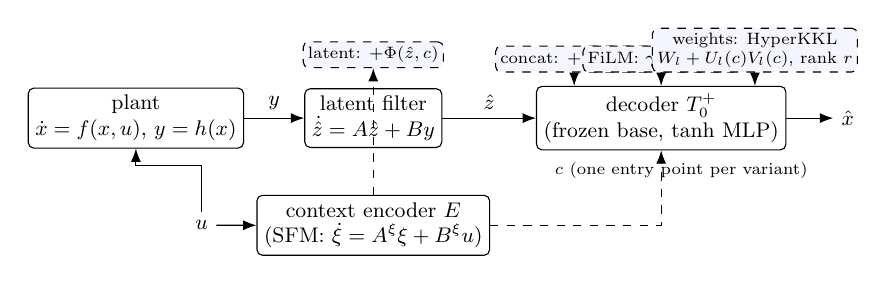
\begin{tikzpicture}[>=Latex, scale=0.85, transform shape, node distance=4mm and 6mm, every node/.style={font=\small},
  box/.style={draw, rounded corners=2pt, minimum height=7mm, inner sep=3pt, align=center},
  cond/.style={draw, dashed, rounded corners=2pt, inner sep=2pt, font=\scriptsize, align=center, fill=blue!4}]
\node[box] (plant) {plant\\$\dot x=f(x,u)$, $y=h(x)$};
\node[box, right=9mm of plant] (filt) {latent filter\\$\dot{\hat z}=A\hat z+By$};
\node[box, right=14mm of filt] (dec) {decoder $T_0^+$\\(frozen base, tanh MLP)};
\node[right=7mm of dec] (xh) {$\hat x$};
\node[box, below=7mm of filt] (enc) {context encoder $E$\\(SFM: $\dot\xi=A^\xi\xi+B^\xi u$)};
\node[left=6mm of enc] (u) {$u$};
\draw[->] (plant) -- node[above]{$y$} (filt);
\draw[->] (filt) -- node[above]{$\hat z$} (dec);
\draw[->] (dec) -- (xh);
\draw[->] (u) -- (enc);
\draw[->] (u) |- ($(plant.south)+(0,-2.5mm)$) -- (plant.south);
\node[cond, above=2mm of filt.north, yshift=1mm] (L) {latent: $+\Phi(\hat z,c)$};
\draw[->, dashed] (enc.north) -- ++(0,2mm) -| (L.south);
\node[cond, above=2mm of dec.north, xshift=-13mm] (C) {concat: $+R([\hat z,c])$};
\node[cond, above=2mm of dec.north, xshift=0mm] (F) {FiLM: $\gamma_l(c),\beta_l(c)$};
\node[cond, above=2mm of dec.north, xshift=14mm] (W) {weights: HyperKKL\\$W_l+U_l(c)V_l(c)$, rank $r$};
\draw[->, dashed] (enc.east) -| ($(dec.south)+(0,0)$);
\node[font=\scriptsize, below=0.5mm of dec.south, xshift=3mm] {$c$ (one entry point per variant)};
\draw[->, dashed] (C.south) -- (dec.north -| C.south);
\draw[->, dashed] (F.south) -- (dec.north -| F.south);
\draw[->, dashed] (W.south) -- (dec.north -| W.south);
\end{tikzpicture}
\caption{The HyperKKL framework. Solid: the parts shared by every variant (filter, frozen base decoder, context encoder). Dashed: the entry points of the input context $c$; HyperKKL is the weight-space entry (rank-$r$ updates $U_lV_l$ written by a hypernetwork of $c$), the other three are the compared alternatives. The deployed latent is an input-free linear filter for every decoder-side variant; only the latent variant changes the dynamics.}
\label{fig:framework}
\end{figure}

\paragraph{What the theory says, informally.} The full statements and proofs are in Appendices~\ref{sec:m1}--\ref{sec:m3}; three results frame the experiments. Each is tagged with what it proves.

\emph{C1: where the input enters is a stability--extrapolation trade-off} (Proposition~\ref{prop:m1-where}, proven). Latent injection makes the observer a recurrent system whose stability depends on the input: the error contracts only if $\mu_2(A+\partial_z\Phi(z,\hat c))\le-\mu<0$ on a set fixed in advance, the certified margin shrinks with the context (Corollary~\ref{cor:m1-amplitude}), and there are bounded, observable plants with an \emph{exact} injection whose latent observer diverges at a fixed filter spectrum (Proposition~\ref{prop:m1-tight}). Decoder-side conditioning keeps the latent an input-free stable filter, so stability holds for every input, but the decoder is queried at unseen contexts and its excess error there is at best linear in the distance to the training contexts (Corollary~\ref{cor:m1-ood}). The theory does \emph{not} rank concat, FiLM and the weight-space generators (Remark~\ref{rem:m1-capacity}), which is why C1 is an experiment.

\emph{C2: a short input window suffices} (Lemma~\ref{lem:m2-tail}, Theorem~\ref{thm:m2-window}). The finite-start map and the map that sees only the last $L$ seconds of input differ by at most $\tfrac12\varepsilon(L)$, $\varepsilon(L)=2\kappa\|B\|\bar y\,e^{-\alpha L}/\alpha$, so a window $L^*\le(\ln(1/\eta)+\ln\ell+\mathrm{const})/\alpha$ is \emph{sufficient} for a relative error $\eta$, with $\ell$ the Lipschitz constant of the inverse of the windowed map (Corollary~\ref{cor:m2-rule}). Necessity is proven for linear plants only, and the counterfactual-past argument behind it does not apply to the chaotic plants. The pre-registered C2 rules dropped $\ln\ell$; Section~\ref{sec:c2} reports that they fail.

\emph{C3: a wrong model leaves a bias floor that no data lowers} (Proposition~\ref{prop:m3-mismatch}, proven for linear plants). A fixed-gain predict--correct filter built on a model that lacks a term $d$ has error $e_{k+1}=(I-KC)Fe_k+(I-KC)(d_k+w_k)-Kv_{k+1}$, hence a non-decaying bias and a bias--variance floor $\inf_K\mathrm{MSE}(K)>0$ that inflating the process covariance (what the oracle-tuned filters do) can only trade against noise; the floor depends on the model error and on no data. A decoder trained on the true plant pays its fit error, in which no model term appears (Proposition~\ref{prop:m3-iss}). Prediction: a single crossing in the relative model error. On the nonlinear benchmarks this is the reading of an \emph{empirical} result. The ISS bound of Proposition~\ref{prop:m3-iss} is an exact decomposition with measured constants; a priori it is vacuous on every benchmark and is not offered as a certificate.

\section{Experimental design}\label{sec:design}

The protocol was fixed before the reported runs, in the form of an \emph{experiment tree}: each node is a YAML file with a question, a hypothesis, a configuration diff and a \emph{decision rule}; the rules are applied by a script to the finished runs and the verdict (PASS, FAIL, REPORTED for descriptive rules, INCONCLUSIVE or PENDING while jobs are missing) is printed without hand editing (Table~\ref{tab:decisions}). Table~\ref{tab:protocol} summarises the protocol; the rest of this section defines its terms.

\begin{table}[t]
\centering\small
\setlength{\tabcolsep}{4pt}
\caption{Protocol summary (design constants from \texttt{configs/base.yaml} and the node files; no results). A ``cell'' is one plant $\times$ tier $\times$ condition block; every method is evaluated on the same episodes of a cell (paired).}
\label{tab:protocol}
\begin{tabular}{@{}p{0.2\textwidth}p{0.77\textwidth}@{}}
\toprule
plants & 12 (Table~\ref{tab:systems}): 6 \emph{dev} (every design decision) and 6 \emph{test} (held out; run once with the frozen recipe, no tuning). Each set spans 2-D, 3-D chaotic and $\ge4$-D plants. \\
inputs & bounded box $v(t)\in[-1,1]$ by construction, through a saturating actuator; times in units of a per-plant $t_\mathrm{ref}$. Tiers: \tier{id} (training families, fresh seeds), \tier{shape\_ood} (waveforms never trained on: chirp, filtered noise, triangle, sawtooth; same box and band), \tier{sequence\_ood} (the ``drive'' family with a stop-and-go event sequence; same level grid). \\
knowledge & what every model-based component (phase-1 PDE term, filters, oracle model-error rate) is given: \emph{exact}; \emph{mismatch} $p\%$ (real plant's parameters $p\%$ off nominal, $p\in\{10,20,30,50\}$); \emph{partial} (one physical term missing or simplified, Table~\ref{tab:systems}); \emph{realistic} (partial $+$ 30\% $+$ coloured Student-$t$ noise). The real plant keeps its full dynamics and generates every label. \\
conditions & \tier{clean} (nominal sensor: white Gaussian, 3\% of each output's reference std); sensor faults (noise, outliers, dropout, coloured, coloured Student-$t$, quantised, drift, burst outage); input faults (noise, bias, delay); poor initialisation; post-training plant drift (10\%, 30\%). No observer is told about a condition. \\
learned observers & autonomous (no context), HyperKKL and the three alternative entry points of Section~\ref{sec:framework}, one frozen base per plant and seed, conditioner budget 140k (controls at 35k and 560k; hyper subspace $k=1/4/16$, Table~\ref{tab:capacity}), SFM context (dim 16, 8 blocks), HyperKKL rank $r=4$ (ablations $r=1,16$ and the dense-subspace generator); NLOX, a neural Luenberger observer with a learned input-affine latent term \citep{woelk2026}, trained on the same data. All need full-state labels. \\
model-based filters & EKF, UKF, PF (512 particles), \texttt{kkl\_mb} (the stationary-transformation controlled KKL observer of \citet{bernard2019luenberger}: learned autonomous maps with the model's exact input correction $\partial_xT_0(\hat x)[f(\hat x,u)-f(\hat x,0)]$ in the latent dynamics); robust \texttt{ekf\_huber}, \texttt{ukf\_huber} (Huber update, nominal $Q,R$); condition-oracle \texttt{ekf\_oracle}, \texttt{ukf\_oracle} (rebuilt per condition with its sensor statistics and a $Q$ that includes the model-error rate; inflation factors chosen on validation episodes). Filters hold the modeller's model and never see state labels. \\
reference lines & \emph{climatology}: NRMSE of the constant mean-state predictor, same normalisation; a filter above it is FAILED and never used as a comparator. EKF on the exact model as the accuracy reference for C1. \\
data & per plant and seed: 400 zero-input episodes (phase 1), 600 forced training episodes, 64 validation episodes (model selection only), 64 evaluation episodes per tier; steady window = second half of each episode. \\
seeds, statistics & the training seed is the unit of replication: 5 seeds for \node{C1-where}, \node{C3-faults} and \node{C3-realistic}, 3 for every other node and for the test plants. Paired Student-$t$ 95\% CIs over per-seed relative changes; ``A beats B'' = CI excludes 0 in A's favour. Control nodes add a TOST equivalence test at $\pm10\%$ (90\% CI) \citep{schuirmann1987tost}. System-level rules count plants ($k/6$) and are not corrected for multiplicity. \\
\bottomrule
\end{tabular}
\end{table}

\paragraph{Plants.} Table~\ref{tab:systems} (Appendix~\ref{app:tables}) lists the twelve plants with the state and output dimensions, the latent dimension $n_z$, where the input enters, the term that the \emph{partial} model lacks, and the resulting relative model error $\mathrm{median}\,\|f_\mathrm{real}-f_\mathrm{model}\|/\|f_\mathrm{real}\|$ over the operating box. Dev: \sys{battery}, \sys{bioreactor}, \sys{duffing}, \sys{lorenz}, \sys{quad\_tank} \citep{johansson2000}, \sys{vdp}. Test: \sys{cartpole}, \sys{fhn} \citep{fitzhugh1961}, \sys{highway\_traffic}, \sys{network} (five coupled neurons, three measured), \sys{rossler} \citep{rossler1976}, \sys{two\_link\_arm}.


\paragraph{What out-of-distribution means.} A deployed estimator sees inputs inside the actuator's range; what changes is the waveform's \emph{shape} or the event \emph{sequence} (another driver, another road). Every family in every tier realises $v(t)\in[-1,1]$ without clipping and training covers the whole box, so no tier changes the amplitude and the evaluation states lie inside the training box (Appendix~\ref{app:protocol}). An earlier amplitude-OOD protocol was abandoned for driving bounded plants beyond their input range (Appendix~\ref{app:history}).

\paragraph{Metrics.} $\nrmse=\sqrt{\mathrm{mean}_{t\in S}\mathrm{mean}_j (e_j(t)/\sigma_j)^2}$ on the steady window $S$, with $\sigma_j$ the reference std of state $j$ under in-distribution inputs of the nominal plant, fixed once per plant (one yardstick for every method, tier and condition); normalised errors are clipped at 100 so a diverged episode contributes a bounded value and is flagged. The deployment scorecard adds per block the quantities of Section~\ref{sec:scorecard}.

\paragraph{Selection and comparison rules.} ``Best learned'' is the lowest mean NRMSE among HyperKKL, its dense ablation and latent injection in a cell, ``best filter'' the lowest among the eight filters (nominal and robust/oracle reported separately); both are selected on the evaluation episodes, which favours the side with more candidates. A rule that names no tier must pass on \tier{shape\_ood} and \tier{sequence\_ood} separately; \tier{id} is reported. The reading rules are printed in full in Appendix~\ref{app:protocol}.

\paragraph{Transparency.} The held-out C1 runs come from four code snapshots (a recorded data problem, Appendix~\ref{app:history}; the recipe was frozen); control nodes have 2--3 seeds, at which ``within CI'' can hardly fail, hence the TOST column. Two baselines trained on the same labels (a Koopman Kalman filter on an EDMD-with-inputs lift; a grey-box EKF/UKF with a learned residual) are implemented and marked pending in Section~\ref{sec:c3}. Nodes not discussed in the text carry their verdicts in Table~\ref{tab:decisions} (learning curves \node{C3-data50/150}: \OutcomeCThreeDataFifty, \OutcomeCThreeDataOneFiveZero, descriptive, partially finished).
% TODO (pending baselines): koopman_kf / koopman_kf_bilinear / greybox_ekf (hyperkkl reeval) are
% NOT in paper/generated at the time of writing; add to the filter list and to C3 only once they
% appear in RESULTS.md / numbers.tex.

\section{C1: where should the input enter?}\label{sec:c1}

\paragraph{Question and rule.} With the same frozen base maps, the same SFM context and a 140k-parameter conditioner, which entry point generalises best to unseen input shapes and sequences? Pre-registered rule (\node{C1-where}): a location is \emph{preferred} if it beats every other location with a paired 95\% CI excluding 0 on $\ge4/6$ dev plants, on \tier{shape\_ood} and \tier{sequence\_ood} separately, and is significantly worse on none. The weaker statement named by the hypothesis, ``weight-space (the better of HyperKKL and its dense ablation) beats both latent and concat on $\ge4/6$'', was pre-registered as the rule for the held-out plants (\node{TEST-C1}, run once with the frozen recipe).

\begin{figure}[t]
\centering
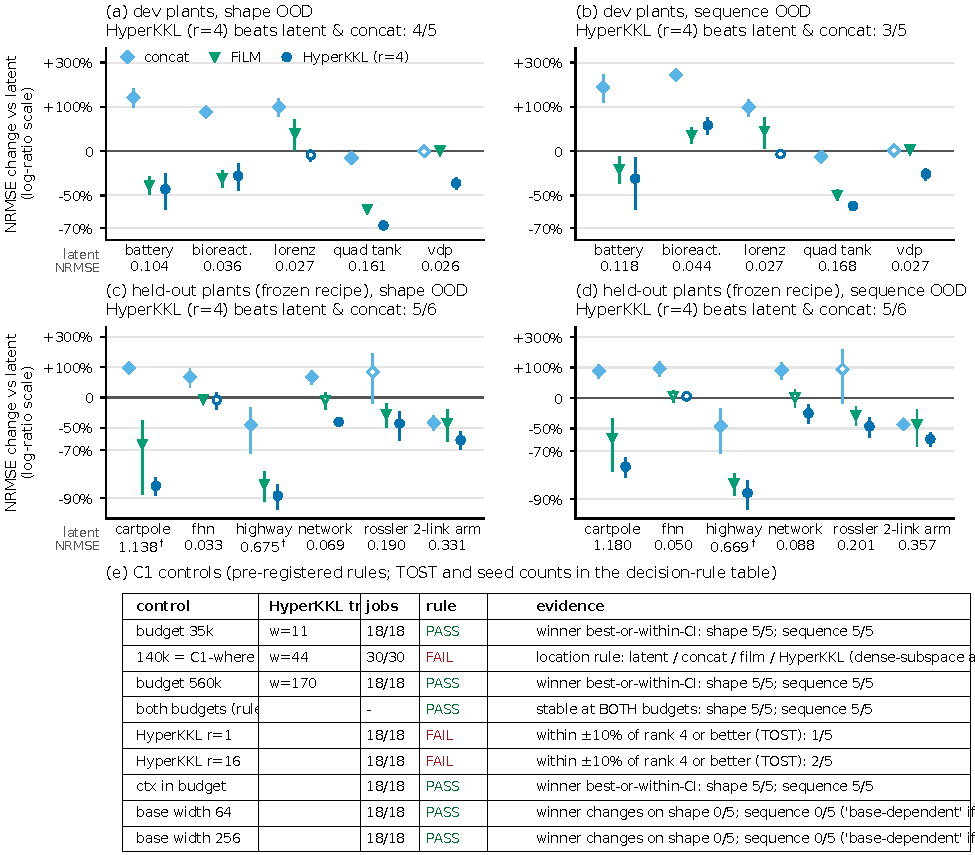
\includegraphics[width=0.68\textwidth, trim=0 171 0 0, clip]{fig1_c1_where.pdf}
\caption{C1, paired change in NRMSE relative to latent injection (the reference; its absolute NRMSE is printed under each plant). (a,b) dev plants, 5 seeds; (c,d) held-out plants, frozen recipe, 3 seeds. Filled markers: 95\% CI over seeds excludes 0; bars: 95\% CI. $\dagger$: latent injection itself above climatology. The pre-registered single-location rule fails on the dev plants (panel (e) of the generated figure, reproduced as Table~\ref{tab:decisions}); the weight-space-beats-latent-and-concat rule passes in all four panels.}
\label{fig:c1}
\end{figure}

\paragraph{Verdict: the pre-registered rule fails; the weaker claim holds and replicates.} No location is preferred (\node{C1-where}: \OutcomeCOneWhere; preferred location: \ConePreferredLocation): HyperKKL beats every other location on \ConeLoraBeatsAllShape\ plants (\tier{shape\_ood}) and \ConeLoraBeatsAllSeq\ (\tier{sequence\_ood}), its dense ablation on \ConeHyperBeatsAllShape\ and \ConeHyperBeatsAllSeq, and the two are within each other's CIs on most plants (Figure~\ref{fig:c1}; absolute NRMSE in Table~\ref{tab:c1}, Appendix~\ref{app:tables}). The weaker claim holds: weight-space beats both latent and concat on \ConeWeightSpaceBeatsLatConcShape\ (\tier{shape\_ood}) and \ConeWeightSpaceBeatsLatConcSeq\ (\tier{sequence\_ood}) plants. Read for HyperKKL alone ($r=4$) against latent injection: better on \ConeLoraBeatsLatentShape\ and worse on \ConeLoraLosesLatentShape\ plants on \tier{shape\_ood} (\ConeLoraVsLatentRangeShape\ where significant), better on \ConeLoraBeatsLatentSeq\ and worse on \ConeLoraLosesLatentSeq\ on \tier{sequence\_ood} (the loss is \sys{bioreactor}, where latent injection is best); FiLM is better on \ConeFilmBeatsLatentShape\ and worse on \ConeFilmLosesLatentShape, the additive residual \ConeConcatBeatsLatentShape\ and \ConeConcatLosesLatentShape. On the held-out plants (\node{TEST-C1}: \OutcomeTESTCOne) the weight-space claim holds on \CtestWeightSpaceBeatsLatConcShape\ and \CtestWeightSpaceBeatsLatConcSeq; HyperKKL alone beats latent injection on \CtestLoraBeatsLatentShape\ and \CtestLoraBeatsLatentSeq\ plants (\CtestLoraVsLatentRangeShape\ where significant), the exception being \sys{fhn}, where it is within CI of latent injection; latent injection is above climatology on \sys{cartpole} and \sys{highway\_traffic} (\tier{shape\_ood}), where HyperKKL is not. No single location passes the strict rule (\CtestPreferredLocation).
% TODO (results layer, single-method re-reading): replace the LoRA-named macros above by the
% 'hyperkkl' macros and add the HyperKKL-vs-concat count once generated; the weight-space verdicts
% (\ConeWeightSpaceBeatsLatConc*, \CtestWeightSpaceBeatsLatConc*) are the pre-registered ones.

\paragraph{Controls.} Each control is a pre-registered node whose counts are in Table~\ref{tab:decisions}. The ranking survives when the context encoder is charged to the budget (\node{C1-ctx}: \OutcomeCOneCtx) and across budgets of 35k and 560k (\node{C1-budget}: \OutcomeCOneBudget; an asterisk, where printed, marks a verdict decided while seeds were running). \emph{Rank ablation.} The rank is a real knob: $r=1$ and $r=16$ are not equivalent to $r=4$ at the $\pm10\%$ margin (\node{C1-rank1}: \OutcomeCOneRankOne, \node{C1-rank16}: \OutcomeCOneRankSixteen; Table~\ref{tab:decisions}), with $r=1$ losing accuracy on the chaotic and the oscillatory plant and $r=16$ non-inferior or better on half of them, consistent with $r$ trading regularisation against capacity; the default $r=4$ is the pre-registered setting, not a tuned one. Base-width controls (winner not base-dependent): \OutcomeCOneBasewidthSixtyFour\ / \OutcomeCOneBasewidthTwoFiveSix\ (jobs \JobsCOneBasewidthSixtyFour, \JobsCOneBasewidthTwoFiveSix). The model-free phase-1 control (\node{C1-modelfree}; rule: the model is needed if the PDE-regularised base wins on $\ge4/6$) reads \OutcomeCOneModelfree: no evidence that the phase-1 model term is needed (Table~\ref{tab:decisions}).

\paragraph{Reference: with an exact model the EKF is far better.} The best learned observer's \tier{sequence\_ood} NRMSE is \ConeLearnedOverEkfMedianSeq$\times$ the exact-model EKF's (median over dev plants; range \ConeLearnedOverEkfRangeSeq$\times$) and \CtestLearnedOverEkfMedianSeq$\times$ on the held-out plants (\CtestLearnedOverEkfRangeSeq$\times$); C1 ranks learned observers, whether to learn at all is C3.

\paragraph{Caveats.} (i) Vote counts are descriptive (5 variants $\times$ 2 tiers $\times$ 6 plants, no multiplicity correction) and the ``better of HyperKKL/ablation'' selection in the weight-space verdicts is made on the evaluation episodes. (iii) The dense-subspace ablation generates full-shape updates inside a fixed linear subspace of dimension $k=1$, $4$ and $16$ at the 35k, 140k and 560k budgets, while HyperKKL's rank-4 factors are bilinear in a 11-, 44- and 170-dimensional trunk feature (Table~\ref{tab:capacity}); its tie with HyperKKL is a tie between these parameterisations. (iv) The latent variant is trained through 256-step rollouts at the same learning rate and steps, so location is confounded with trainability for it, and decoder-side gains could partly be repair of a weak base map; a learning-rate search and a context-swap control are not in the tree. (v) In-distribution results (Table~\ref{tab:c1-id}) show the same ordering.

\section{C3: when does a learned KKL observer beat a model-based filter?}\label{sec:c3}

\paragraph{Question and rules.} The best KKL observer (HyperKKL, its dense ablation or latent injection, as pre-registered) is compared with the best of eight model-based filters, paired on the same episodes, on \tier{id} and \tier{sequence\_ood}; ``learned wins'' in a scenario needs a CI excluding 0 on $\ge4/6$ dev plants on both tiers. The filters hold the modeller's model; the learned observers are trained on labelled data from the real plant. Absolute NRMSE accompanies every change; a filter above \emph{climatology} is FAILED, and changes are quoted against the best \emph{working} filter with the number of failed filters. Scenarios: exact model under fifteen stress conditions (\node{C3-faults}, descriptive), coloured Student-$t$ noise in training and deployment (\node{C3-noise-ct}), parameter mismatch at four levels (\node{C3-mismatch10/20/30/50}; hypothesis: the crossover sits between 10\% and 30\%), a missing physical term (\node{C3-partial}, descriptive, against the relative model error), and the realistic deployment (\node{C3-realistic}).

\begin{figure}[t]
\centering
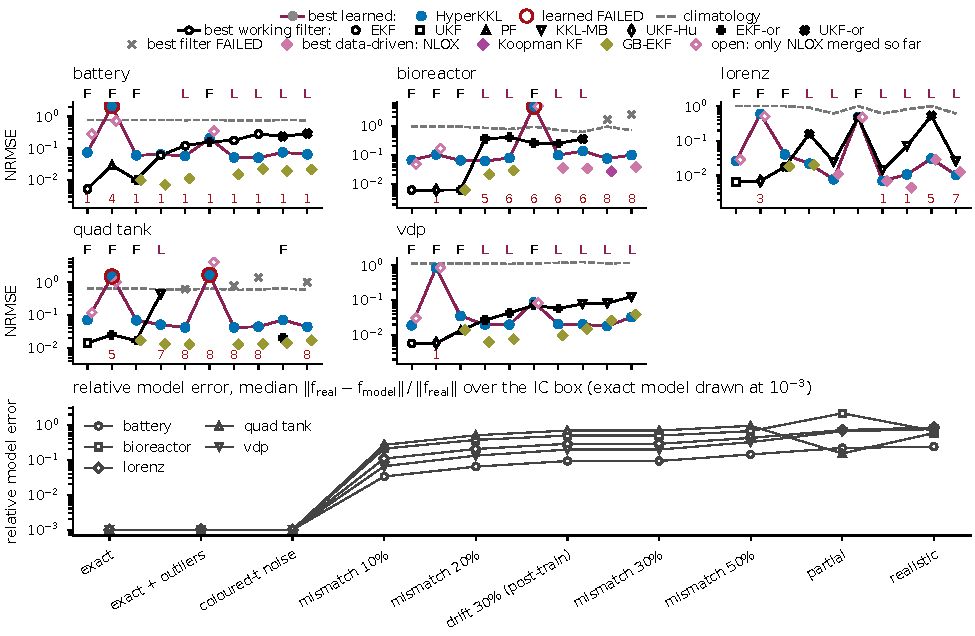
\includegraphics[width=0.68\textwidth, trim=0 140 0 0, clip]{fig3_c3_crossover.pdf}
\caption{C3 on the dev plants, \tier{sequence\_ood}, NRMSE on a log axis: best learned observer (coloured by method) against the best working filter (black) and climatology (dashed), per scenario ordered by the median relative model error over plants (the model-error panel of the generated figure is omitted here; the values are in Table~\ref{tab:systems} and in Figure~\ref{fig:c3id}). Top marks: L = learned beats the best working filter (paired 95\% CI), F = filter wins; red numbers = filters above climatology. Red-ringed markers: the best \emph{learned} observer is itself above climatology. Grey crosses: the best filter is FAILED and there is no working filter. The \tier{id} version and the held-out plants are in Appendix~\ref{app:tables}.}
\label{fig:c3}
\end{figure}

\paragraph{Exact model: the filters win everywhere.} In none of the fifteen stress conditions does the learned side reach the learned-wins regime (\node{C3-faults}: \CthreeFaultsRegimes), against nominal and robust/oracle filters alike (Tables~\ref{tab:c3} and \ref{tab:decisions}). Under coloured heavy-tailed noise in training and deployment the learned observers beat the best filter on \CthreeNoiseCtSeqVsWorking\ plants (\node{C3-noise-ct}: \OutcomeCThreeNoiseCt). Two exact-model failures of the learned observers: under 2\% gross sensor outliers the best learned observer is itself above climatology on \sys{battery}, \sys{duffing} and \sys{quad\_tank}, while the Huber and oracle filters keep their clean accuracy (Table~\ref{tab:c3full}); and after a 30\% plant drift that occurs \emph{after} training, it is above climatology on \sys{bioreactor} and \sys{quad\_tank}. These limits of the method as trained here (nominal sensor, no robust loss, no adaptation) are consistent with the theory: the fault's effect is multiplied by a decoder slope in the hundreds (Corollary~\ref{cor:m3-faults}, Remark~\ref{rem:m3-cert}), and on linear plants a Kalman filter beats any KKL observer with outliers too (Remark~\ref{rem:m3-kf}).

% generated by analysis/paper_results.py -- do not edit by hand
% requires \usepackage{booktabs,longtable,array}
\begin{table}[t]
\centering
\scriptsize
\setlength{\tabcolsep}{2pt}
\caption{When does a learned KKL observer win (C3)? sequence OOD, dev plants: number of plants on which HyperKKL ($r=4$, the single learned method) beats the comparator (paired 95\% CI excludes 0). Per-plant numbers: Table~\ref{tab:c3full}.}
\label{tab:c3}
\begin{tabular}{@{}lrrrrrrrr@{}}
\toprule
 & & \multicolumn{5}{c}{(a) vs model-based filters} & \multicolumn{2}{c}{(b) vs data-driven} \\
\cmidrule(lr){3-7}\cmidrule(l){8-9}
scenario & model err. & best filter & working & nominal & rob./orac. & failed & best data-driven & NLOX \\
\midrule
exact & 0.00 & 0/5 (5L) & 0/5 (5L) & 0/5 (5L) & 0/5 (5L) & 1/40 & pend.\ 0/25 & 3/5 \\
exact+outliers & 0.00 & 0/5 (5L) & 0/5 (5L) & 0/5 (5L) & 0/5 (5L) & 14/40 & pend.\ 0/25 & 1/5 (3L) \\
colored\_t & 0.00 & 0/5 (5L) & 0/5 (5L) & 0/5 (5L) & 0/5 (5L) & 1/40 & 0/5 (5L) & 4/5 \\
mismatch10 & 0.11 & 4/5 & 4/5 & 4/5 & 4/5 & 13/40 & 0/5 (4L) & 3/5 \\
mismatch20 & 0.20 & 5/5 & 4/4$^*$ & 5/5 & 5/5 & 15/40 & 1/5 (4L) & 4/5 (1L) \\
drift30 (post-train) & 0.29 & 0/5 (4L) & 0/4 (4L)$^*$ & 2/5 (2L) & 1/5 (4L) & 15/40 & pend.\ 0/25 & 2/5 (1L) \\
mismatch30 & 0.29 & 5/5 & 4/4$^*$ & 5/5 & 5/5 & 16/40 & 0/5 (3L) & 3/5 \\
mismatch50 & 0.42 & 5/5 & 4/4$^*$ & 5/5 & 5/5 & 16/40 & 0/5 (3L) & 3/5 \\
partial & 0.66 & 4/5 (1L) & 3/4 (1L)$^*$ & 4/5 (1L) & 4/5 (1L) & 14/40 & 1/5 (3L) & 3/5 (1L) \\
realistic & 0.68 & 5/5 & 3/3$^*$ & 5/5 & 5/5 & 24/40 & 2/5 (3L) & 4/5 (1L) \\
\bottomrule
\end{tabular}
\par\smallskip\begin{minipage}{\linewidth}\scriptsize ($k$L): the comparator is significantly better on $k$ plants. (a) Model-based filters: EKF, UKF, PF, KKL-MB and their Huber and oracle variants. A filter is FAILED when its NRMSE exceeds climatology (the constant mean-state predictor); `working' = the best filter that did not fail ($^*$: no filter works on some plants). (b) Data-driven baselines trained on the same real-plant data: NLOX, Koopman KF (incl.\ bilinear), grey-box EKF/UKF/EKF-oracle; `pend.\ $m/N$' = merged in $m$ of $N$ runs. Model error: median over dev plants.\end{minipage}
\end{table}


\paragraph{Wrong model: the learned observers win at every level tested.} With the real plant's parameters off nominal, the learned side beats the best filter on \CthreeMismatchTenIdVsWorking\ (\tier{id}) and \CthreeMismatchTenSeqVsWorking\ (\tier{sequence\_ood}) plants at 10\% (\OutcomeCThreeMismatchTen), \CthreeMismatchTwentyIdVsWorking\ and \CthreeMismatchTwentySeqVsWorking\ at 20\% (\OutcomeCThreeMismatchTwenty), \CthreeMismatchThirtyIdVsWorking\ and \CthreeMismatchThirtySeqVsWorking\ at 30\% (\OutcomeCThreeMismatchThirty), \CthreeMismatchFiftyIdVsWorking\ and \CthreeMismatchFiftySeqVsWorking\ at 50\% (\OutcomeCThreeMismatchFifty); the same counts hold against the robust/oracle filters, which are given the model-error rate in $Q$. The pre-registered crossover hypothesis therefore \FAIL s (\node{C3-mismatch (crossover)}: \OutcomeCThreeMismatchCrossover): the first winning level is the smallest one tested, and the crossing, if there is one, lies below 10\%. The exception at every level is \sys{duffing}, whose 30\% parameter error moves $f$ by only \ModelErrDuffingMismatchThirty\ in relative terms (Table~\ref{tab:systems}) and whose best filter stays several times better (\CthreeMismatchThirtySeqDuffingBestWorking\ against \CthreeMismatchThirtySeqDuffingBestLearned\ at 30\%); \sys{battery} at 10\% is the other non-win on \tier{sequence\_ood} (\CthreeMismatchTenSeqBatteryVsWorking, n.s.). With one physical term missing (\node{C3-partial}: \OutcomeCThreePartial), the learned side wins on \CthreePartialIdVsWorking\ and \CthreePartialSeqVsWorking\ plants; the exception is \sys{quad\_tank}, where linearising the orifice law moves $f$ by \ModelErrQuadTankPartial\ and the oracle EKF wins (\CthreePartialSeqQuadTankBestWorking\ against \CthreePartialSeqQuadTankBestLearned), whereas \sys{bioreactor} (relative model error \ModelErrBioreactorPartial), \sys{lorenz} (\ModelErrLorenzPartial) and \sys{vdp} (\ModelErrVdpPartial) are won at every level and \sys{duffing} (\ModelErrDuffingPartial) is won here. The pattern hypothesised for this node (learned wins on \sys{bioreactor}/\sys{vdp}/\sys{lorenz}, filters on \sys{duffing}/\sys{quad\_tank}) holds on four of its five named plants (Table~\ref{tab:decisions}).

\paragraph{Realistic deployment.} With partial model, 30\% parameter error and coloured Student-$t$ noise at once, the learned observers win on \CthreeRealisticIdVsWorking\ (\tier{id}) and \CthreeRealisticSeqVsWorking\ (\tier{sequence\_ood}) plants against the best filter of any kind and against the best working filter (\node{C3-realistic}: \OutcomeCThreeRealistic). On \sys{bioreactor} and \sys{quad\_tank} all eight filters are above climatology (\CthreeRealisticSeqBioreactorFailedFilters, \CthreeRealisticSeqQuadTankFailedFilters), so no change is quoted: the learned observers reach \CthreeRealisticSeqBioreactorBestLearned\ and \CthreeRealisticSeqQuadTankBestLearned\ against climatology \CthreeRealisticSeqBioreactorClimatology\ and \CthreeRealisticSeqQuadTankClimatology. On \sys{lorenz} \CthreeRealisticSeqLorenzFailedFilters\ filters fail and the working one, \texttt{kkl\_mb}, is beaten by \CthreeRealisticSeqLorenzVsWorking; \sys{battery}, \sys{duffing} and \sys{vdp} by \CthreeRealisticSeqBatteryVsWorking, \CthreeRealisticSeqDuffingVsWorking\ and \CthreeRealisticSeqVdpVsWorking.

\paragraph{Reading the crossover.} Over the 36 model-wrong cells (six plants $\times$ mismatch 10--50\%, partial, realistic), every non-win sits at a small relative model error (\sys{duffing}, \sys{battery} at 10\%, \sys{quad\_tank} partial) and every plant with a large error is won at every level (Figure~\ref{fig:c3}, Table~\ref{tab:c3full}): the single crossing Proposition~\ref{prop:m3-mismatch} predicts, at a plant- and noise-dependent value (Appendix~\ref{sec:m3}).

\paragraph{Two findings, not one.} (a) \emph{Learning from real-plant data beats model-based filters once the model is wrong.} This is the robust finding: it holds against nominal, robust and oracle-tuned filters, at every mismatch level, under a missing term and in the realistic node, and it reverses whenever the model is exact. (b) \emph{Which learner wins is system-dependent and is not settled here.} Two further estimators trained on exactly the learned observers' data are implemented: \texttt{koopman\_kf} (EDMD with inputs on a thin-plate-RBF dictionary, then a Kalman filter on the lifted state) and \texttt{greybox\_ekf/ukf} (the modeller's model plus an MLP residual fitted to the one-step defect, inside the unchanged EKF/UKF). This comparison (b), best KKL observer against the best data-driven baseline (NLOX included), was added after review and is \emph{not} pre-registered; it is merged into the runs node by node (column (b) of Table~\ref{tab:c3}). Where it is complete enough to decide, \node{C3-partial}, the KKL observers do \emph{not} win: \OutcomeCThreePartialDataDriven\ (KKL beats the best data-driven baseline on \CthreePartialIdVsDataDriven\ plants on \tier{id} and \CthreePartialSeqVsDataDriven\ on \tier{sequence\_ood}): on \tier{sequence\_ood} the grey-box EKF/UKF is better on \sys{battery} (\CthreePartialSeqBatteryBestDataDriven\ against \CthreePartialSeqBatteryBestLearned) and \sys{duffing} (\CthreePartialSeqDuffingBestDataDriven\ vs \CthreePartialSeqDuffingBestLearned), the Koopman KF on \sys{bioreactor}, and the KKL observers are better on \sys{lorenz} (\CthreePartialSeqLorenzVsDataDriven\ vs NLOX) and \sys{vdp} (\CthreePartialSeqVdpVsDataDriven\ vs the grey-box EKF). For the mismatch, realistic and held-out nodes comparison (b) is \OutcomeCThreeRealisticDataDriven\ at the time of writing (merge counts in Table~\ref{tab:c3}). So \emph{no claim that the KKL observer is the best learner is made}.
% TODO (pending, 05:07 / 08:07 Dubai regeneration): once koopman_kf / greybox_* appear in
% paper/generated (tab2_c3*.tex, numbers.tex), replace the sentence above by the generated counts
% (learned KKL vs same-data baselines, paired CI) and update the abstract, Section 1 item 2 and
% Section 9 accordingly. Never state a winner that the generated tables do not show.
Nor does C3 establish that the partial model helps the learned observer: the pre-registered test of the phase-1 PDE term with the partial model against a model-free phase 1 \FAIL s (\node{C3-partial-modelfree}: \OutcomeCThreePartialModelfree; the differences are not significant at three seeds, including a large but non-significant one on \sys{bioreactor}), so no claim that the partial model helps is made. Whether the KKL observers' structural advantages (global convergence, no linearisation) show against the grey-box filters where they should, under a poor initial guess, outliers, higher noise, post-training drift and a sensor outage with partial knowledge, is the question of a further node, \node{C3-regimes} (pre-registered rule: a KKL-wins regime needs $\ge4/6$ dev plants per condition on \tier{sequence\_ood}), whose outcome is \textcolor{red}{\textbf{\OutcomeCThreeRegimes}} at the time of writing. The replication on the held-out plants (\node{TEST-C3}, the realistic scenario) is \OutcomeTESTCThree\ at the time of writing with \JobsTESTCThree\ jobs finished: the learned side wins on \sys{fhn} (\CthreeTESTCThreeSeqFhnVsWorking\ on \tier{sequence\_ood}) and \sys{highway\_traffic} (\CthreeTESTCThreeSeqHighwayTrafficVsWorking), the UKF wins on \sys{cartpole} (\CthreeTESTCThreeSeqCartpoleVsWorking) although its realistic model error (partial \ModelErrCartpolePartial, 30\% \ModelErrCartpoleMismatchThirty) is comparable to that of dev plants the learned side won; with half the plants finished, no reading of the held-out crossover is offered.
% TODO (pending results): TEST-C3 is refreshed by the 05:00 / 08:00 regeneration; re-read this
% paragraph and the abstract sentence on held-out C3 once the node is decided.

\section{Supporting analysis (C2): how much input history does the decoder need?}\label{sec:c2}

The theory says that a window of $\ln(1/\eta)/\alpha$ plus a plant-dependent $\ln\ell/\alpha$ is sufficient. Three pre-registered tests were run on the dev plants; all three \FAIL\ and are reported as supporting analysis.

\paragraph{Forgetting floor.} The SFM context was forced to forget at a rate $\ge c\alpha$, $c\in\{0.25,0.5,1\}$ (\node{C2-floor-025/05/1}). Rule (decided at $c=0.5$): no significant loss relative to the un-floored context for HyperKKL and its dense ablation, on \tier{id} and \tier{sequence\_ood}, on $\ge5/6$ plants, and the memory probe must decay at least at the floor rate. Outcome: \OutcomeCTwoFloorFive: no-loss on \CtwoFloorFiveNoLoss\ plants (TOST at $\pm10\%$: \CtwoFloorFiveTostNonInferior; three seeds make ``no significant loss'' weak evidence), probe at or above the floor rate on \CtwoFloorFiveProbeAboveFloor\ (Figure~\ref{fig:c2floor}, Appendix~\ref{app:tables}). The dose--response is monotone: at $c=0.25$, \CtwoFloorTwentyFiveNoLoss\ (\OutcomeCTwoFloorTwentyFive\ on the TOST and probe parts); at $c=1$, \CtwoFloorOneNoLoss\ (\OutcomeCTwoFloorOne). The one plant that clearly loses at $c=0.5$ is \sys{battery} (HyperKKL \CtwoFloorFiveBatteryLoraId\ on \tier{id}, \CtwoFloorFiveBatteryLoraSeq\ on \tier{sequence\_ood}; \CtwoFloorOneBatteryLoraId\ at $c=1$), the plant with the largest decoder-Lipschitz proxy ($\ell_{\rm dec,q95}=\CtwoLdecQBattery$ against \CtwoLdecQLorenz--\CtwoLdecQDuffing\ elsewhere): its state of charge enters the voltage only through the open-circuit-voltage slope, so inverting the windowed map costs a large $\ell$ and a longer window, as Corollary~\ref{cor:m2-rule} says. The \sys{bioreactor} loss has no such explanation. Without a floor the learned SFM's slowest pole sits at \CtwoSfmPoleOverAlphaDuffingLora--\CtwoSfmPoleOverAlphaBatteryLora\,$\alpha$ (HyperKKL), between the two slowest \emph{initial} poles ($\alpha/1.5^5=0.13\alpha$, $0.20\alpha$): the un-floored memory is inherited from the initialisation, not learned.

\paragraph{Memory probe.} The last $L$ input samples are kept and everything older is swapped for another episode's input; the decoded change is fitted to a rate (the quantity Lemma~\ref{lem:m2-sfm}(c) bounds). Under a $0.5\alpha$ floor the fitted rate is \CtwoFloorFiveProbeRatioDuffing--\CtwoFloorFiveProbeRatioQuadTank\ of the floor on five plants (no contradiction of an upper envelope, but the strict check fails) and \sys{lorenz}'s probe does not decay at all (\CtwoFloorFiveProbeRatioLorenz; Figure~\ref{fig:c2probe}), which is unexplained and reported as such.

\paragraph{Window sweeps.} With HyperKKL on a raw window of $L$ samples in place of the SFM context (\node{C2-window-a1}), the rule ``$e(L)$ within 5\% of $e(512)$ for every $L\ge L^*=\ln(1/\eta)/\alpha$, $\eta=0.05$, on $\ge5/6$ plants'' gives \OutcomeCTwoWindowAOne: \CtwoWindowTheoryId\ (\tier{id}) and \CtwoWindowTheorySeq\ (\tier{sequence\_ood}) among the evaluable plants (\sys{quad\_tank}'s $L^*=\CtwoLstarQuadTank$ exceeds the grid). The $\ell$-free rule fails where $\ell$ is largest: on \sys{battery} ($L^*=\CtwoLstarBattery$) the error at $L=256$ is still \CtwoWindowTwoFiveSixVsMaxBatterySeq\ above $e(512)$; restoring $\ln\ell$ ($L^*=\CtwoLrefinedBattery$) moves the rule to \CtwoWindowRefinedId\ and \CtwoWindowRefinedSeq\ on the three plants where it stays on the grid, a \emph{post hoc} explanation, not a passed test. Measured knees are far below either rule where they exist (\sys{vdp} \CtwoKneeVdpSeq, \sys{duffing} \CtwoKneeDuffingSeq\ samples), as a sufficient-side bound allows; \sys{bioreactor} is non-monotone. The second-bandwidth test of the $1/\alpha$ scaling (\node{C2-window-a2}, three plants at $2\alpha$) gives \OutcomeCTwoWindowATwo: the knee in samples moved by $\le2\times$ on one of two evaluable plants, so the scaling is not supported by the current data.

\paragraph{What survives.} The sufficient-side statement is consistent with every sweep and the floor costs nothing significant on four of six plants; not established are that memory beyond the theory window is unnecessary, the $1/\alpha$ scaling, and the probe rate. The intervention and the probe remain cheap, reusable diagnostics.

\section{C4: the testbed and the deployment scorecard}\label{sec:scorecard}

Every evaluation block stores a \emph{deployment scorecard}: NRMSE per tier and on the \emph{unmeasured} states, worst sensor-fault NRMSE, p99 and divergence rate, convergence from a far-corner prior and the paired ``forget the prior'' time, recovery after a burst outage, long-horizon drift, the AUROC of an output-residual alarm for the method's own large errors, and time per step (Appendix~\ref{app:protocol}). Figure~\ref{fig:scorecard} (Appendix~\ref{app:tables}) ranks every method on every column over the dev plants for the exact-model stress node and the realistic node (values per plant: Table~\ref{tab:scorecard}).

With an exact model the nominal and oracle filters take the top ranks on accuracy, tails, unmeasured states, convergence and recovery; the learned observers rank better only on the divergence rate (they never diverge; the EKF and UKF sometimes do) and, with the particle filter, on the residual alarm. In the realistic deployment the learned KKL observers take the top ranks on every accuracy column, every filter is above climatology on three of six plants, and the learned observers' alarm is no better than the filters'; time per step is the batched-harness cost, not an embedded number.

The released testbed comprises the twelve plants with their partial-knowledge models, the input protocol, the eight filters with their tuning rules, the climatology reference, the memory probe, the experiment tree with its rules and the script that applies them (Table~\ref{tab:decisions}), and the regeneration path from raw runs to every number here.

\section{Real-data validation: battery SOC on held-out drive cycles}\label{sec:realdata}

C1 and C3 were tested once on real hardware with a design pre-registered before any training (Appendix~\ref{app:realdata}): the Panasonic 18650PF drive cycles \citep{kollmeyer2018panasonic} at 25$^\circ$C, split by cycle: Cycles 1--3, UDDS and LA92 for training, Cycle 4 for validation (model selection, rank-4-vs-dense-ablation choice, filter tuning), and US06, HWFET and NN as test cycles reported once. The target is the laboratory coulomb count ($Q=\RealQAh$\,Ah); the modeller's model is a constant-parameter 2-RC circuit identified by least squares on the training cycles (open-loop voltage RMSE \RealVmFitTrainMin--\RealVmFitTrainMax\,mV there, \RealVmFitValTestMin--\RealVmFitValTestMax\,mV on validation/test), used for phase~1 and inside the EKF/UKF ($Q,R$ tuned on the validation cycle). Episodes are 30-min windows through each discharge from a prior SOC 20\% off; the metric is settled SOC RMSE; a cycle counts only if the 95\% block-bootstrap CI of the paired difference excludes 0 and all \RealNSeeds\ seeds agree.

Both pre-registered rules are met (Table~\ref{tab:real}, Appendix~\ref{app:realdata}); they were decided on ``WS-best'', the per-seed validation choice between HyperKKL ($r=4$) and its dense ablation. H1 (C3): WS-best beats the tuned EKF on \RealHOneLearnedBetter\ of \RealNTestCycles\ test cycles (US06 \RealWsBestEkfUSZeroSixDiff, HWFET \RealWsBestEkfHWFETDiff, NN \RealWsBestEkfNNDiff\,\% SOC; likewise against the UKF), and HyperKKL at $r=4$ alone on \RealLoraEkfCyclesABetter\ of \RealNTestCycles. H2 (C1): WS-best beats latent injection on \RealHTwoWsBetter\ of \RealNTestCycles\ (by \RealWsBestLatentDiffMinAbs--\RealWsBestLatentDiffMaxAbs\,\% SOC, a small margin); HyperKKL at $r=4$ alone passes the strict rule on \RealLoraLatentCyclesABetter\ of \RealNTestCycles\ cycles with the same sign everywhere, and the simulated ordering weight-space $>$ latent $>$ concat $\gg$ autonomous holds. The mechanism is that of C3: on the aggressive US06 cycle the filters settle on a biased SOC (\RealEkfUSZeroSixRmse\,\% against \RealWsBestUSZeroSixRmse\,\%) because the constant-parameter circuit cannot explain the voltage error; the decoder trained on real data can. The limits matter as much: on whole discharges the filters have hours to converge and the gap closes except on US06 (EKF \RealWholeEkfNN\ vs learned \RealWholeWsBestNN\,\% on NN), so on mild cycles the advantage is mostly faster convergence; at 0$^\circ$C, where nothing was trained or identified, the Arrhenius-scaled EKF is better on \RealZeroEkfBetter\ of \RealZeroNCycles\ cycles (learned \RealZeroWsRmseMin--\RealZeroWsRmseMax\,\%); one cell, one campaign; a coulomb-counting reference; a quickly identified circuit model. The same-data baselines (Koopman KF, grey-box EKF) on the real cycles are \textcolor{red}{\textbf{\RealSameDataBaselines}}.
% TODO (pending): when experiments/real/results.json contains koopman_kf / greybox_* rows, re-run
% analysis/real_numbers.py (\RealSameDataBaselines flips to "present"), and report the comparison from
% Table tab:real; never claim the KKL observer is the best learner unless that table shows it.

\section{Related work}\label{sec:related}

\paragraph{KKL observers.} The construction goes back to \citet{kazantzis1998}; \citet{andrieu2006existence} proved existence of the injective map under backward distinguishability, \citet{bernard2017} addressed the inverse, \citet{bernard2019luenberger} extended the theory to non-autonomous plants (history-dependent map), and \citet{brivadis2023further} settled the generic latent dimension ($2n_x+1$ autonomous, $2n_x+2$ time-varying). \texttt{kkl\_mb} is that line's stationary-transformation controlled observer; Remark~\ref{rem:m1-exist} states what is cited and what is assumed.

\paragraph{Learned KKL and neural Luenberger observers.} Learning $T$ and its inverse from simulated data was proposed by \citet{ramos2020} and developed by \citet{janny2021,peralez2021,peralez2022,niazi2023,buisson2023} and \citet{niazi2025kkl} (physics-informed training with robustness guarantees, whose phase-1 recipe we use). \citet{peralez2024} learn KKL observers model-free from data with a switching scheme, for autonomous systems; for driven plants, \citet{woelk2026} learn a Luenberger observer with an input-affine latent term (our NLOX baseline). Our preprint \citep{shaaban2026hyperkkl} introduced hypernetwork conditioning of the KKL maps; this paper replaces its comparisons by a matched, pre-registered study.

\paragraph{Conditioning mechanisms.} FiLM \citep{perez2018film}, hypernetworks \citep{ha2016,chauhan2024} and low-rank adaptation \citep{hu2022}, whose factorised form HyperKKL's generated updates take, are the conditioning families compared here; \citet{zeng2024expressive} analyse the expressive power of low-rank adaptation. Context-generated parameters for dynamical systems appear in CoDA \citep{kirchmeyer2022coda} and HyperPINN \citep{belbuteperes2021hyperpinn}.

\paragraph{Koopman operators with inputs.} The KKL map is the resolvent of the Koopman generator at the filter poles (Remark~\ref{rem:m1-koopman}); latent injection with a stationary map is a lifted Koopman model with inputs and NLOX its bilinear form. DMD with control \citep{proctor2016dmdc}, EDMD \citep{williams2015edmd}, Koopman linear predictors with inputs \citep{korda2018linear}, learned linear embeddings \citep{lusch2018deep} and Koopman observers \citep{surana2016koopman} are the model class the decoder-side route must be compared with on the same data; our EDMD-with-inputs Kalman filter is that comparison (Section~\ref{sec:c3}).

\paragraph{Sequence models and learned filtering.} Neural CDEs \citep{kidger2020neuralcde}, ODE-RNNs and latent ODEs \citep{rubanova2019latentode,chen2018neuralode} are universal encoders of input histories; the SFM context is a fixed fading-memory filter bank in the spirit of \citet{boyd1985fading} with a guaranteed forgetting rate (Lemma~\ref{lem:m2-sfm}); a matched neural-CDE encoder is not in the tree. Learned Kalman filters such as KalmanNet \citep{revach2022kalmannet} and Backprop KF \citep{haarnoja2016backpropkf} learn the gain or the model inside a Kalman structure from labels; our grey-box EKF is the simplest member of that family (Section~\ref{sec:c3}). The classical comparators are the EKF, UKF \citep{julier2004unscented}, bootstrap particle filter \citep{gordon1993novel} and Huber-type robust updates \citep{huber1964robust}.

\section{Limitations}\label{sec:limitations}

\emph{Labels.} Every learned observer, NLOX included, is trained on full-state trajectories of the real plant; C3 is about a practitioner with a wrong model \emph{and} labelled data (a virtual sensor with laboratory ground truth), not model-free estimation. \emph{Exact models.} With an exact model a tuned EKF is \ConeLearnedOverEkfMedianSeq$\times$ better on the dev plants and the filters win every stress condition: if the model is right, do not learn. \emph{Fragility.} Trained on the nominal sensor, the learned observers are above climatology under gross outliers and 30\% post-training drift, where robust filters are not; robust losses, fault augmentation and adaptation are not studied. \emph{Same-data baselines.} The Koopman-KF and grey-box comparison is post hoc and complete on one node, where they beat the KKL observers on three of five plants; C3 is about learning from real-plant data, not the KKL structure. \emph{Capacity.} HyperKKL's tie with its dense-subspace ablation is at $r=4$ and $k=4$; $r=1$ and $16$ are not equivalent (open controls: Section~\ref{sec:c1}). \emph{Statistics.} Control nodes have 2--3 seeds (most TOST cells underpowered); vote counts are uncorrected for multiplicity; best-of selections use the evaluation episodes. \emph{Chaotic plants.} The theory's counterfactual-past statements do not apply to \sys{lorenz} and \sys{rossler}; \sys{lorenz}'s probe is flat and unexplained; \sys{rossler} is weakly chaotic; whether the forced plants stay chaotic was not verified. The held-out \sys{network} plant is weakly observable. \emph{Real data.} One cell, one campaign, one temperature; coulomb-counting reference; a quickly identified circuit model; on whole discharges the filters match the learned observers on mild cycles. \emph{Theory.} The ISS bound is vacuous a priori; the window lower bound and the C3 proposition are linear results whose nonlinear reading is empirical; predictions no node measures are stated as untested.

\paragraph{Broader impact.} A learned observer that beats a filter when the model is wrong can make soft sensing cheaper where laboratory ground truth exists; the same results caution against deploying one where the model is good, sensors produce gross outliers or the plant drifts after training, and its residual alarm is no better than a filter's, so none of these observers should run in a safety-critical loop without a fallback filter. No personal data is used; the compute is a few hundred GPU-hours.

\section{Conclusion}\label{sec:conclusion}

KKL theory requires an input-dependent observer map for a forced plant; where a learned observer should carry it, and when learning one is worth it, were open. On twelve plants with pre-registered rules, the input should enter the decoder's \emph{weights}, as HyperKKL's rank-$r$ updates, rather than the latent dynamics or an additive residual (\ConeWeightSpaceBeatsLatConcShape/\ConeWeightSpaceBeatsLatConcSeq\ dev, \CtestWeightSpaceBeatsLatConcShape/\CtestWeightSpaceBeatsLatConcSeq\ held-out plants), while the single-best-location rule failed because HyperKKL ties with its dense-subspace ablation. Learned observers lose to model-based filters in every exact-model condition (about \ConeLearnedOverEkfMedianSeq$\times$ against a tuned EKF) and win once the model is wrong, at every mismatch level, under a missing term and in a realistic deployment; on real battery drive cycles both orderings replicate (small margin over latent injection; no transfer to an untrained temperature); which learner wins once the model is wrong is system-dependent and, where decided, favours a grey-box EKF. The fading-memory analysis failed its pre-registered tests.


\bibliographystyle{style/tmlr}
\bibliography{refs}

\clearpage
\appendix
% The theory (theory/m1-m3) issues its own \appendix before Lemma D; it is neutralised here so
% that this document has a single \appendix and the theory sections become Appendices A-C.
\section*{Appendix overview}
\addcontentsline{toc}{section}{Appendix overview}

Appendices~\ref{sec:m1}--\ref{sec:m3} are the theory, included unchanged from the maintained source (\texttt{theory/m1\_existence\_location.tex}, \texttt{m2\_fading\_memory.tex}, \texttt{m3\_error\_bounds.tex}; numerical checks in \texttt{theory/checks/*.py}, all of which pass). They are self-contained: Appendix~\ref{sec:m1} states the one assumption block (A1)--(A4) used everywhere, the decoder target, the Koopman reading and the stability--extrapolation trade-off (C1); Appendix~\ref{sec:m2} the fading-memory lemma, the window theorem, the practical rule and the context encoders (C2); Appendix~\ref{sec:m3} the ISS decomposition of the deployed sampled-data observer, the sensor-fault corollary, the Kalman-filter remark, the model-incompleteness proposition that anchors C3, and the single sampled-data lemma (Lemma~D). Every statement carries a status tag ([proven], [proven, linear plants], [conjecture], [empirical]) and names the experiment node that tests it or says that none does. Empirical numbers quoted inside the theory are the same generated macros as in the main text.

Appendix~\ref{app:protocol} gives the protocol details (signal families, training recipe, filter tuning, scorecard definitions, the reading rules of the results layer). Appendix~\ref{app:tables} holds the generated tables and figures not shown in the main text (in-distribution C1 table, per-plant C3 tables for both tiers, the \tier{id} and held-out versions of the C3 figure, the memory probe and window sweeps, the realistic-deployment scorecard, every decision rule with its verdict, and the capacity table of the conditioners). Appendix~\ref{app:history} records what was tried, superseded or abandoned, and the data problems recorded by the results layer.

\paragraph{Reading guide for the theory (status table).}
\begin{center}\footnotesize
\begin{tabular}{@{}p{0.42\textwidth}p{0.2\textwidth}p{0.33\textwidth}@{}}
\toprule
statement & status & tested by \\
\midrule
Lemma~\ref{lem:m1-window}, Prop.~\ref{prop:m1-suff} (decoder target, sufficient contexts, history necessary) & proven & -- \\
Prop.~\ref{prop:m1-where} (latent injection: contraction margin; decoder side: stable, pays extrapolation) & proven & no node measures the margin or the realised gains (eval-only) \\
Cor.~\ref{cor:m1-amplitude}, Prop.~\ref{prop:m1-tight} (margin sufficient only; cannot be removed at a fixed spectrum) & proven & numerical checks \\
Cor.~\ref{cor:m1-ood} (OOD excess $\le$ Lipschitz extrapolation in context distance) & proven & context distance per tier not reported \\
Lemma~\ref{lem:m2-tail} (fading-memory tail; (b) not for chaotic plants) & proven & -- \\
Thm.~\ref{thm:m2-window} (window rule; (b) linear plants) & (a) proven; (b) linear; nonlinear (b) conjecture & \node{C2-window-a1} \OutcomeCTwoWindowAOne, \node{C2-window-a2} \OutcomeCTwoWindowATwo \\
Cor.~\ref{cor:m2-rule} (rule with $\ln\ell$) & proven; its use on the sweep is post hoc & explains the failures post hoc \\
Prop.~\ref{prop:m2-current} (current input not enough) & proven & $L=1$ row of \node{C2-window-a1} \\
Lemma~\ref{lem:m2-sfm} (SFM forgets at a guaranteed rate; (c) = the memory probe) & proven & probe rate $\ge$ floor: \CtwoFloorFiveProbeAboveFloor \\
Prop.~\ref{prop:m3-iss} (ISS relative to the nominal observer) & (i),(ii),(iv) exact; (iii) decomposition & realised gains not measured by any node \\
Cor.~\ref{cor:m3-faults} (sensor faults bounded and forgotten) & proven & \node{C3-faults}: filters win in \CthreeFaultsRegimes \\
Prop.~\ref{prop:m3-mismatch} (bias floor vs fit error) & proven, linear plants & \node{C3-mismatch10--50} PASS, \node{C3-partial}, \node{C3-realistic} \OutcomeCThreeRealistic; \node{TEST-C3} \OutcomeTESTCThree \\
Rem.~\ref{rem:m3-kf} (KF beats KKL on linear plants, also with outliers) & proven & -- \\
Lemma~\ref{lem:D} (sampled-data observer) & proven & checks \\
\bottomrule
\end{tabular}
\end{center}

{\let\appendix\relax
% =====================================================================
% Block M1 (contribution C1): shared assumptions, decoder target, where the input enters.
% Owns: Assumption ass:m1 (A1)-(A4) used by every block, eq:m1-TL, def:m1-suff, lem:m1-window,
% prop:m1-suff, rem:m1-koopman, rem:m1-capacity, prop:m1-where, cor:m1-amplitude, prop:m1-tight, cor:m1-ood.
% Cites: lem:m2-tail, thm:m2-window, prop:m2-current, lem:m2-sfm (block M2); lem:D, prop:m3-iss, prop:m3-mismatch (block M3).
% Checks: paragraph "Numerical checks" at the end of this section (theory/checks/m1_location.py, check_theory.py).
% Status legend used in all three sections: [proven] / [proven, linear plants] / [conjecture] / [empirical].
% =====================================================================
\section{Where the input enters a learned KKL observer}\label{sec:m1}

\paragraph{Setting and conventions.} Plant $\dot x=f(x,u)$, $y=h(x)$, $x\in\mathbb R^{n_x}$,
$y\in\mathbb R^{n_y}$; no input-affine structure. Inputs are applied through a zero-order hold at the
sample rate with values in a compact $U\ni0$, $\bar u:=\max_{U}|u|$; $u_t$ is the window $u|_{[t-L,t]}$
shifted to $[-L,0]$, a point of $W_L=U^{N_L}$ at sample instants when $L/dt=N_L\in\mathbb N$ (the decoder
runs only there), with the sup norm. $X(x,t;s;u)$ is the value at $s$ of the solution through $x$ at $t$.
The latent filter is $\dot z=Az+By$. \emph{Latent initial condition (one convention for Sections
\ref{sec:m1}--\ref{sec:m3}).} The \emph{label} and training latents start from $z(0)=0$, so
$z(t)=T^0(x(t),t;u):=\int_0^te^{A(t-s)}Bh(X(x(t),t;s;u))\,ds$ exactly; this finite-start map is the only
time-varying map used. The \emph{deployed} observer (decoder-side and latent-injection alike, \texttt{evaluate.py}
\texttt{z0\_map}) starts from $\hat z(0)=\hat T_0(\hat x_0)$, which adds the transient $e^{At}\hat T_0(\hat x_0)$ to
the latent; it is carried as the $\Delta z_0$ term of Proposition~\ref{prop:m3-iss} and never absorbed into a map.
The decoder target is the windowed map
\begin{equation}\label{eq:m1-TL}
T_L(x,w):=\int_{-L}^{0}e^{-A\tau}B\,h\big(X(x,0;\tau;w)\big)\,d\tau,
\end{equation}
which by Lemma~\ref{lem:m2-tail}(a) is within $\tfrac12\varepsilon(L)$ of $T^0(x(t),t;u)$ at $w=u_t$.
$\mathcal P_L$ is the set of pairs $(x(t),u_t)$, $t\ge L$, generated by admissible trajectories.

\begin{assumption}[standing; shared by all sections]\label{ass:m1}
Regularity: $f(\cdot,u)\in C^1$ uniformly in $u\in U$, $h\in C^2$.
\begin{enumerate}
\item[(A1)] \emph{Forward invariance.} A compact $\mathcal X$ contains every solution from the initial set
  $\mathcal X_0\subset\mathcal X$ under every admissible input, for all $t\ge0$.
\item[(A2)] \emph{Bounded output.} $\|h(x)\|\le\bar y$ on $\mathcal X$.
\item[(A3)] \emph{Hurwitz filter.} $-\alpha<0$ is the spectral abscissa of $A$ and
  $\kappa:=\sup_{t\ge0}e^{\alpha t}\|e^{At}\|<\infty$ ($\kappa=1$ for the normal Butterworth $A$ of the code).
\item[(A4)] \emph{Uniform Lipschitz injectivity of the windowed map.} There are $L_0$ and $\ell<\infty$ with
  $|x_1-x_2|\le\ell\,|T_L(x_1,w)-T_L(x_2,w)|$ for all $(x_1,w),(x_2,w)\in\overline{\mathcal P_L}$ and all
  $L\ge L_0$ (i.e.\ $\ell:=\sup_{L\ge L_0}\ell(L)<\infty$; Theorem~\ref{thm:m2-window}(a) varies $L$ at fixed $\ell$).
\end{enumerate}
\end{assumption}
\noindent\emph{Chaotic plants.} (A1)--(A3) hold for the dissipative chaotic benchmarks (Lorenz, R\"ossler), (A4) is
assumed for them as for every other plant, but its constant is not under control when $\alpha$ is below the
\emph{backward} expansion rate $\lambda_b$ of the flow (for Lorenz $\lambda_b\approx14.6$ against $\alpha=2$):
$\partial_xT^0$ contains $\int_0^te^{A(t-s)}B\,\partial h\,\partial_xX(x,t;s;u)\,ds$ and $\|\partial_xX\|$ grows like
$e^{\lambda_b(t-s)}$ along the backward flow, so the forward Lipschitz constant of $T^0(\cdot,t)$ grows with $t$ when
$\alpha<\lambda_b$; this is the eigenvalue condition of \citet{andrieu2006existence} (the spectrum of $A$ must
dominate the Lipschitz constant of $f$ for a $C^1$ stationary map; a H\"older map needs less), and it is a plausible
mechanism (not tested: no node sweeps $\alpha$ or measures $\lambda_b$) behind the phase-1 PDE residual
$\varepsilon_{\rm pde,rms}=74$ on Lorenz against $\le0.3$ elsewhere. Which results survive on such plants is stated at
each result: everything that uses only the true past and (A1)--(A2) does (Lemma~\ref{lem:m2-tail}(a),
Theorem~\ref{thm:m2-window}(a), Proposition~\ref{prop:m3-iss}); the counterfactual-past statements
(Lemma~\ref{lem:m2-tail}(b)) and the linear lower bounds (Theorem~\ref{thm:m2-window}(b),
Proposition~\ref{prop:m2-current}(b)) do not apply to them.

\begin{remark}[existence and injectivity: cited, and what is assumed]\label{rem:m1-exist}
$T^0$ is a $C^1$ solution of $\partial_xT\,f(x,u(t))+\partial_tT=AT+Bh(x)$ whenever backward solutions
exist on $[0,t]$ \citep[Lemma~1]{bernard2019luenberger}, and an observer
$\hat x=T^*(\hat z,t)$ converges if there are $\bar t$ and a concave class-$\mathcal K_\infty$ $\rho_T$ with
$|x_1-x_2|\le\rho_T(|T(x_1,t)-T(x_2,t)|)$ for all $t\ge\bar t$ \citep[Theorem~1]{bernard2019luenberger}.
For a fixed input that is backward distinguishable in finite time, $T^0(\cdot,t)$ is injective for almost
every complex diagonal $A$ with $n_y(n_x+1)$ eigenvalues \citep[Theorem~3]{bernard2019luenberger}, but the
exceptional set depends on the input \citep[Remark~5]{bernard2019luenberger}; the Lipschitz, uniform-in-time
version \citep[Theorem~2]{bernard2019luenberger} needs strong differential observability, inputs of class
$C^{m+1}$ (their time derivatives enter) and a gain $k$ above a threshold, which excludes held, switching
and PRBS inputs and a fixed $(A,B)$. For autonomous systems, $2n_x+1$ generic real dimensions suffice
\citep[Theorem~3.4]{brivadis2023further}, $2n_x+2$ for time-varying ones \citep[Remark~3.6]{brivadis2023further}.
(A4) is therefore \emph{assumed}: it is the quantitative, uniform-in-input version of what these results give
for each regular input. The code's $n_z=5$ for 2-D plants is the autonomous count; the time-varying count
$2n_x+2$ is not met, so (A4) at $n_z=5$ is an assumption whose constant must be reported, not a consequence of the cited
results; the phase-1 proxy for $\ell$ (\texttt{l\_dec\_q95}, Remark~\ref{rem:m3-cert}) is $24$ (vdp), $44$
(bioreactor), $299$ (duffing), $10$ (lorenz), $14$ (quad\_tank), $816$ (battery) for the C1-where phase~1 (used in
\texttt{check\_apriori\_vacuity}); the C2-window-a1 phase~1 of the results layer gives $23,44,295,10,14,806$
(Table~\ref{tab:m2-window-rule}).
\end{remark}

\begin{remark}[Koopman reading; which model classes the variants are]\label{rem:m1-koopman}
For the autonomous plant and a diagonalised filter $A=\mathrm{diag}(\lambda_i)$, $B=(b_i)$, the KKL PDE
$\partial_xT_i\,f=\lambda_iT_i+b_ih$ reads $(L_f-\lambda_i)T_i=b_ih$ with $L_f=f\cdot\nabla$ the Koopman generator on
observables, so
\[
T_i=b_i\,(L_f-\lambda_i)^{-1}h=b_i\int_0^\infty e^{\lambda_i\tau}\,h\big(X(x,0;-\tau;0)\big)\,d\tau ,
\]
the resolvent of the generator at the filter pole, i.e.\ the Laplace transform of the backward Koopman semigroup
applied to the output observable; if $h=\sum_jc_j\varphi_j$ with $L_f\varphi_j=\mu_j\varphi_j$ then
$T_i=\sum_jb_ic_j\varphi_j/(\mu_j-\lambda_i)$. For a linear plant this is the row identity
$p_i=b_iC(F-\lambda_iI)^{-1}$ of the Sylvester solution (check [7]); for a nonlinear plant it gives the spectral
reading of the ``$A$ fast enough'' condition above ($\operatorname{Re}\lambda_i$ must clear the backward spectrum) and of
the zero-input floor $\varepsilon_0$ of Remark~\ref{rem:m1-capacity}(i) as a spectral truncation. Under an input the
same object is the resolvent for the skew-product (state $\times$ input-shift) system, and the windowed map $T_L$ is its
finite-horizon version with the window as a truncated coordinate on the shift space; for a linear plant the context
$\dot q=Aq-PGu$ of Proposition~\ref{prop:m1-suff}(a) has the structure of a linear predictor with inputs
\citep{proctor2016dmdc,korda2018linear}. In these terms, \emph{latent injection} with a stationary $T_0$ is a lifted
Koopman model with inputs (its input-affine case $\Omega(z)u$, and the NLOX baseline $\omega(z)u$, are bilinear lifted
observers with a fixed output-injection gain $B$), whose stability requires the input-dependent generator $A+\partial_z\Phi$
to stay contracting (Proposition~\ref{prop:m1-where}(a)); \emph{decoder-side conditioning} keeps a fixed generator and
parametrises the left inverse of the lifting by the input context. Proposition~\ref{prop:m1-tight} is then the
statement that the Koopman spectrum moves with $u$ (eigenvalue $u-a$; rotation rate $\omega_0+u$) while a fixed $A$ does
not. We state this as positioning only; no result below depends on it.
\end{remark}

\subsection{The decoder target and sufficient contexts}

\begin{definition}[sufficient context]\label{def:m1-suff}
A context map $E:W_L\to\mathbb R^{d_c}$ is \emph{sufficient} if the latent and the context determine the state:
for $(x_i,w_i)\in\overline{\mathcal P_L}$, $E(w_1)=E(w_2)\Rightarrow|x_1-x_2|\le\ell\,|T_L(x_1,w_1)-T_L(x_2,w_2)|$.
It is $\epsilon_E$-sufficient if the same holds with an additive $\epsilon_E$ on the right.
\end{definition}
\noindent The window itself ($E=\mathrm{id}$) is sufficient by (A4). A lower-dimensional $E$ cannot be
injective on $W_L$ (invariance of domain), but it need not be: it only has to resolve what the latent leaves open.

\begin{lemma}[decoder target]\label{lem:m1-window}
Let $E$ be continuous and $\epsilon_E$-sufficient, and $S_L:=\{(T_L(x,w),E(w)):(x,w)\in\overline{\mathcal P_L}\}$.
If $\epsilon_E=0$ there is a continuous $G^*:S_L\to\mathcal X$ with $G^*(T_L(x,w),E(w))=x$, $\ell$-Lipschitz in $z$
for each $c$; extend $G^*(\cdot,c)$ to $\mathbb R^{n_z}$ with the same constant (Kirszbraun). Then along every
admissible trajectory, for $t\ge L$,
$\ |G^*(z(t),E(u_t))-x(t)|\le\tfrac{\ell}{2}\varepsilon(L).$
For $\epsilon_E>0$, any decoder $D$ satisfies $\sup|D(T_L(x,w),E(w))-x|\ge\tfrac12\delta_E$, where $\delta_E$ is the
largest $|x_1-x_2|$ over pairs with equal latent and equal context.
\end{lemma}
\noindent\emph{Intuition.} Over a fixed window the plant has no clock, so the state is a fixed function of
(latent, context) as soon as the context resolves the latent's ambiguity.
\begin{proof}
$\Psi(x,w)=(T_L(x,w),E(w))$ is continuous on the compact $\overline{\mathcal P_L}$ (under the hold, the backward
solution is a composition of $N_L$ $C^1$ flows with constant parameters). By sufficiency, $\Psi(x_1,w_1)=\Psi(x_2,w_2)$
implies $x_1=x_2$, so $\pi_x$ factors as $G^*\circ\Psi$; $G^*$ is continuous because $\Psi$ is a closed map
(continuous on a compact set into a Hausdorff space), and $\ell$-Lipschitz in $z$ by sufficiency. Then
$|G^*(z(t),c)-x(t)|=|G^*(z(t),c)-G^*(T_L(x(t),u_t),c)|\le\ell\,|z(t)-T_L(x(t),u_t)|$ and Lemma~\ref{lem:m2-tail}(a).
The lower bound: $D$ returns one value for two states $\delta_E$ apart.
\end{proof}

\begin{proposition}[sufficient contexts exist, and must carry history]\label{prop:m1-suff}
(a) \emph{Linear plants.} For $\dot x=Fx+Gu$, $y=Cx$, the windowed map is affine in $x$ with a
$w$-independent slope, $T_L(x,w)=P_Lx+Q_Lw$, $P_L=P-e^{AL}Pe^{-FL}$, $PF=AP+BC$. Hence the $n_z$-dimensional linear
context $c=Q_Lw$ is exactly sufficient whenever $P_L$ is injective ($\ell=\|P_L^+\|$), and as $L\to\infty$ (under the
washout $e^{AL}Pe^{-FL}\to0$, (H1) of Theorem~\ref{thm:m2-window}) it is the
output $q$ of the stable filter $\dot q=Aq-PGu$: a spectral filter bank with identity readout.
(b) \emph{Nonlinear plants.} The window ($d_c=n_uN_L$) is sufficient, and by (a) of Lemma~\ref{lem:m2-tail}
any context that determines $u_t$ for some $L$ is $\ell\varepsilon(L)$-sufficient for the infinite past:
$|x_1-x_2|\le\ell\,|T^0_1-T^0_2|+\ell\,\varepsilon(L)$ (each $T^0_i$ is within $\tfrac12\varepsilon(L)$ of $T_L$).
(c) \emph{History is necessary.} The current input alone is not sufficient in general
(Proposition~\ref{prop:m2-current}).
\end{proposition}
\begin{proof}
(a) $X(x,0;\tau;w)=e^{F\tau}x+(\text{linear in }w)$; substitute in \eqref{eq:m1-TL} and use
$\int_{-L}^0e^{-A\tau}BCe^{F\tau}d\tau=P-e^{AL}Pe^{-FL}$ (integrate $\tfrac{d}{d\tau}(e^{-A\tau}Pe^{F\tau})=e^{-A\tau}BCe^{F\tau}$).
If $Q_Lw_1=Q_Lw_2$ then $T_L(x_1,w_1)-T_L(x_2,w_2)=P_L(x_1-x_2)$. The limit: $z-Px$ obeys $\dot{(z-Px)}=A(z-Px)-PGu$.
(b) (A4) and Lemma~\ref{lem:m2-tail}(a).
\end{proof}
\noindent For nonlinear plants and contexts of fixed dimension below $n_uN_L$, finite stable filter banks with a
static readout uniformly approximate every time-invariant fading-memory operator on slew-limited bounded inputs
\citep[Theorem~2]{boyd1985fading}; applying it to the observer operator $(y,u)\mapsto x$ (a fading-memory operator
under (A1)--(A4), on slew-limited signals, and for the filters the theorem chooses rather than ours) motivates the
spectral context but is not a guarantee for the trained encoder.

\begin{remark}[expressivity at a fixed base; what C1 compares]\label{rem:m1-capacity}
(i) \emph{Shared floor.} Every conditioner with exact zero-input collapse, $D(\cdot,0)=T_0^+$, errs at $c=0$ by
$\varepsilon_0:=\sup_z|G^*(z,0)-T_0^+(z)|$: the zero-input target is the inverse of the zero-input windowed map,
not the learned stationary base. (ii) \emph{Additive (concat).} $T_0^+(z)+R(z,c)-R(z,0)$ approximates on $S_L$, as
the width of $R$ grows, every continuous target that equals $T_0^+$ on the zero slice: SiLU satisfies
$\mathrm{SiLU}(s)-\mathrm{SiLU}(-s)=s$, so a two-hidden-layer SiLU network contains every one-hidden-layer one, and
the universal approximation theorem for non-polynomial activations \citep{leshno1993multilayer} applies (with a
Tietze extension of the target). (iii) \emph{Base-capped (FiLM, LoRA, hypernetwork).} For each fixed $c$ the decoder
is a network $N_{\theta(c)}$ of the frozen base's architecture, so for every conditioner budget
\[
\inf_{D}\ \sup_{S_L}|D-G^*|\ \ge\ \sup_{c}\ \inf_{\theta\in\Theta}\ \sup_z|N_\theta(z)-G^*(z,c)|,
\]
with $\Theta$ the reachable parameter set. At the matched budget $\Theta$ is much smaller than the base's weight
space: the hypernetwork's linear bias-free heads place $\theta(c)$ in an affine subspace of dimension equal to its
trunk width; LoRA updates have the configured rank and leave biases fixed; FiLM never modulates the readout layer, so
$D(\cdot,c)=W_L\phi_c(z)+b_L$ with $(W_L,b_L)$ frozen. In the ReLU setting, a LoRA rank of order width times a depth
ratio suffices to represent a smaller target network exactly \citep{zeng2024expressive}; that result does not cover
tanh bases or small fixed ranks. (iv) \emph{Latent injection.} $\Phi$ is a universal class, but as an observer it
represents only targets of the stationary route: a stationary $T_0$ with an exact correction.
The theory therefore does not rank the variants by expressivity; at a matched budget on one base, C1 measures
inductive bias and optimisation within these classes.
\end{remark}

\subsection{Where the input enters: a stability--extrapolation trade-off}

Both observers run the filter on $y+\nu$, $\|\nu\|_\infty\le\delta_y$, with a context $\hat c=E(\hat u)$ of the input
$\hat u$ they are given; $c=E(u)$ and $\delta_c:=\sup_t|\hat c-c|\le\ell_E\|\hat u-u\|_\infty$ (Lemma~\ref{lem:m2-sfm}).
\begin{align*}
\text{(latent)}\quad &\dot{\hat z}=A\hat z+B(y+\nu)+\Phi(\hat z,\hat c), && \hat x=T_0^+(\hat z),\ \ \hat z(0)=T_0(\hat x_0),\\
\text{(decoder side)}\quad &\dot{\hat z}=A\hat z+B(y+\nu), && \hat x=D(\hat z,\hat c),\ \ \hat z(0)=\hat T_0(\hat x_0).
\end{align*}
For the latent variant, $T_0\in C^1$ is a stationary map with left inverse $T_0^+$ ($\ell_{\rm dec}$-Lipschitz,
$\varepsilon_{\rm dec}=\sup_{\mathcal X}|T_0^+T_0(x)-x|$), the residual along trajectories is
$r=\partial_xT_0(x)f(x,u)-AT_0(x)-Bh(x)-\Phi(T_0(x),c)$ with $|r|\le\varepsilon_{\rm res}$, and $\ell_{\Phi,c}$ is the
Lipschitz constant of $\Phi(z,\cdot)$ \emph{uniformly over} $z\in T_0(\mathcal X)+B(r)$ (the set used in (a)).
$\mu_2(M)=\lambda_{\max}(\tfrac12(M+M^\top))$ is the logarithmic norm.

\begin{proposition}[where the input enters]\label{prop:m1-where}
Under Assumption~\ref{ass:m1}:
\begin{enumerate}
\item[(a)] \emph{Latent injection: stability depends on the input} [proven]. Let
$\bar d:=\varepsilon_{\rm res}+\|B\|\delta_y+\ell_{\Phi,c}\,\delta_c$ and let $r\ge|e(0)|+\bar d/\mu$. If
$\mu_2\big(A+\partial_z\Phi(z,\hat c)\big)\le-\mu<0$ for all $z$ in the set $\mathcal Z_r:=T_0(\mathcal X)+B(r)$ and all
contexts $\hat c$ the observer meets, then $e=\hat z-T_0(x)$ stays in $B(r)$ for all $t$ (so the hypothesis is
checked on a set fixed in advance, not on the solution) and
\[
|e(t)|\le e^{-\mu t}|e(0)|+\tfrac1\mu\big(\varepsilon_{\rm res}+\|B\|\delta_y+\ell_{\Phi,c}\,\delta_c\big),\qquad
|\hat x-x|\le\ell_{\rm dec}|e|+\varepsilon_{\rm dec}.
\]
\item[(b)] \emph{Decoder side: stability is free, extrapolation is not} [proven]. The latent is an input-free LTI filter,
so $\hat z-z$ is driven only by $\nu$ and the initial transient, and $|\hat x-x|$ obeys the bound of
Proposition~\ref{prop:m3-iss} for every input, with the decoder's Jacobian norms $\ell_z(\hat c),\ell_c(\hat c)$ taken at
the contexts actually queried. Both conditioner families have $c$-uniform bounds on a bounded context set, but with very
different constants: for an additive conditioner $\ell_z(c)\le\ell_z(T_0^+)+2\sup\|\partial_zR\|$; for multiplicative
ones (FiLM, LoRA, hypernetwork) the available bound is the product form
$\ell_z(c)\le\prod_l\|W_l+\Delta W_l(c)\|\sup|\sigma'|^{d}$, finite because $\theta(c)$ is bounded (tanh trunk, bounded
$c$), but $10^1$--$10^5$ times larger at random initialisation (check [5]) before the tanh base saturates.
\end{enumerate}
\end{proposition}
\noindent\emph{Intuition.} Injecting the input makes the observer a recurrent network whose stability depends on how
strongly the injection reacts to the latent, but its decoder never sees an unfamiliar context; conditioning the decoder
keeps the recurrent part a fixed stable filter, but the network is queried at every unseen context directly.
\begin{proof}
(a) $\dot e=Ae+[\Phi(\hat z,\hat c)-\Phi(T_0x,\hat c)]+d$, $d=B\nu+[\Phi(T_0x,\hat c)-\Phi(T_0x,c)]-r$, $|d|\le\bar d$. While
$e\in B(r)$ the segment $[T_0x,\hat z]$ lies in the ball $T_0x+B(r)\subseteq\mathcal Z_r$ (convexity of the ball,
not of $\mathcal Z_r$, is what is used); write the bracket as $\bar Je$,
$\bar J=\int_0^1\partial_z\Phi(T_0x+se,\hat c)ds$, so $\mu_2(A+\bar J)\le-\mu$ by subadditivity and convexity of $\mu_2$,
and $D^+|e|\le-\mu|e|+\bar d$. The comparison function $\phi(t)=e^{-\mu t}|e(0)|+\bar d(1-e^{-\mu t})/\mu\le r$ bounds
$|e|$ as long as $e\in B(r)$, and $\phi<r$ whenever $|e|=r$ would be reached, so $B(r)$ is forward invariant and the
bound holds for all $t$ (contraction, \citealp{lohmiller1998contraction}; equivalently the perturbation lemmas of
\citealp[Ch.~9]{khalil2002nonlinear}). The state bound is the triangle inequality through $T_0^+(T_0(x))$.
(b) The latent statement is linearity; the bound is Proposition~\ref{prop:m3-iss}; the Jacobian bounds are the chain rule
($R$'s $z$-Jacobian does not involve $c$ multiplicatively, whereas modulated layers multiply $z$-features by $c$-dependent
weights), and $\theta(c)$ is bounded because the trunk is tanh and $c$ is bounded (Lemma~\ref{lem:m2-sfm}).
\end{proof}

\begin{corollary}[the certified margin shrinks with the context]\label{cor:m1-amplitude}
$\mu_2(A+\partial_z\Phi)\le\mu_2(A)+\ell_\Phi$, and $\mu_2(A)=-\alpha$ for normal $A$, so $\mu\ge\alpha-\ell_\Phi$
(for general $A$, the Gronwall version gives $\alpha-\kappa\ell_\Phi$). For an injection with exact zero-input
collapse, $\Phi(z,c)=M(z,c)-M(z,0)$, $M\in C^2$: $\ell_\Phi(c)\le\min\big(|c|\,L_{zc},\,2\sup\|\partial_zM\|\big)$ with
$L_{zc}=\sup\|\partial_c\partial_zM\|$, and $|c|\le\ell_E\|u\|_\infty$ (sup norm) since $E(0)=0$; for an input-affine
injection $\Omega(z)u$, $\ell_\Phi\le\ell_\Omega\|u\|_\infty$. The margin is evaluated at the \emph{observer's} context
$\hat c$, so a corrupted input shrinks it. The margin saturates: if $2\kappa\sup\|\partial_zM\|<\alpha$ the latent observer
is certified at every amplitude, and when the plant input saturates (as through a saturating actuator) the exact
correction's $z$-Lipschitz constant stays bounded too. The condition is \emph{sufficient only}: for the code's trained
injection the certified margin is already negative at moderate gain ($-5.47$, log-norm $+8.1$ in check [3]) while two
observer copies still contract, so a negative margin predicts nothing, and only a measured incremental rate does.
\end{corollary}

\begin{proposition}[the margin cannot be removed at a fixed spectrum]\label{prop:m1-tight}
[proven] There are bounded, observable plants with an \emph{exact} injection ($\varepsilon_{\rm res}=0$) whose latent
observer diverges while a decoder-side observer with a bounded sufficient context is within $\tfrac{\ell}{2}\varepsilon(L)$
of exact. For $\dot x=(u-a)x+b$, $y=x$, $a>\alpha>0$, scalar latent $\dot z=-\alpha z+y$ and constant $u\in(\alpha,a)$:
the plant converges to $b/(a-u)$, the stationary map is $T_0(x)=Px+q$, $P=1/(\alpha-a)$, $q=-Pb/\alpha$, the exact
injection is $\Phi^*(z,u)=u(z-q)$ ($\ell_\Phi=|u|$), and $\dot e=(u-\alpha)e$. The windowed map is
$T_L(x,w)=P_L(u)\,x+Q_L(u)$ with $P_L=\int_{-L}^0e^{(\alpha+u-a)\tau}d\tau>0$ and
$Q_L=\int_{-L}^0e^{\alpha\tau}\,b\,\tfrac{e^{(u-a)\tau}-1}{u-a}\,d\tau$ (both bounded functions of the window input), so the
decoder $\hat x=(\hat z-Q_L)/P_L$ errs by at most $\tfrac{\ell}{2}\varepsilon(L)$ with $\ell=1/P_L$
(Lemma~\ref{lem:m1-window}), for every $u\in(\alpha,a)$.
\end{proposition}
\begin{proof}
$T_0'(x)f(x,0)=P(b-ax)$ and $-\alpha T_0+x=(1-\alpha P)x-\alpha q=-aPx+Pb$; so $T_0$ solves the zero-input PDE and
$\partial_xT_0[f(x,u)-f(x,0)]=Pux=u(T_0(x)-q)$. Then $\dot e=-\alpha\hat z+x+u(\hat z-q)-P((u-a)x+b)=(u-\alpha)e$.
For the window: $X(x,0;\tau;u)=e^{(u-a)\tau}x+b(e^{(u-a)\tau}-1)/(u-a)$ in \eqref{eq:m1-TL}.
\end{proof}
\noindent Here the small-gain threshold $u=\alpha$ is attained exactly. The \emph{exact} time-varying map $z=m(t)x+n(t)$,
$\dot m=1-(\alpha+u-a)m$, $\dot n=-\alpha n-bm$, is also a sufficient context, but for $u<a-\alpha$ its coefficient
$-(\alpha+u-a)$ is positive and $m,n\to\infty$ (check: $m(30)=2\cdot10^{19}$ at $u=0.5$); it is outside the bounded
class of Proposition~\ref{prop:m1-where}(b), which is why the windowed context is the one used. The obstruction is
intrinsic to the stationary route \emph{at a fixed spectrum}: a designer removes it by choosing $\alpha>\bar u$ (here) or
$\alpha>\bar u\ell_\Omega\kappa$ (Corollary~\ref{cor:m1-amplitude}), i.e.\ by a gain that grows with the input bound, which
is also what \citet[Theorem~4]{bernard2019luenberger} require. A second example, the rotating oscillator
$\dot x=(\omega_0+u)Jx$, $y=x_1$ ($|x|$ is conserved for every input), with the drift map $P$ and the exact correction
$\Omega(z)=PJP^+z$, has error rate $\max\operatorname{Re}\lambda(A+uPJP^+)$: stable for all tested $u>-\omega_0$, but
unstable ($+2.65$, $+5.16$ at $u=-2,-4$, $\omega_0=1$, $n_z=5$, $\alpha=1.5$) when the rotation reverses, although the
plant is bounded and observable there; this is the input-independence required by the stationary route
\citep[Theorem~4]{bernard2019luenberger}, which also needs an input-affine plant and a gain growing with $\bar u$.
The decoder-side route needs only Assumption~\ref{ass:m1} and a sufficient context.

\paragraph{What the bounds predict, and what the current nodes test.} Under protocol v2 no tier changes the input
amplitude (every family lives in the same box), so the quantity that varies between tiers is the \emph{distance in context
space}, $d(\hat c,\mathcal C_{\rm train})$, not $|c|$. (P1) The latent variant's excess error on \texttt{shape\_ood} and
\texttt{sequence\_ood} is the extrapolation error of $\Phi$ at the new contexts, filtered at the measured incremental rate;
it degrades sharply only if that rate approaches zero. Decoder-side variants pay $\ell_z(\hat c)\,|\Delta z|$ and
$\ell_c(\hat c)\,|\Delta c|$ at the new contexts (Corollary~\ref{cor:m1-ood}), with the additive conditioner's $\ell_z$ small
and $c$-uniform. (P2) Input noise moves the latent variant's operating point to a corrupted context $\hat c$ (its margin is
evaluated there), whereas decoder-side variants stay stable for every input and pay $\ell_c\ell_E\delta_u$.
\emph{Status: untested.} No current node measures $\mu_2$ or the incremental rate on visited segments, $\ell_z(\hat c)$,
$\ell_c(\hat c)$, or the context distance per tier; under C3-faults \texttt{input\_noise} every variant, latent included,
degrades by about the same factor ($\approx10\times$ on vdp, read from the C3-faults node report; not a number of the
generated results layer), which neither supports nor falsifies (P2). The quantities to
record are eval-only on saved checkpoints: $\min_{c'\in\mathcal C_{\rm train}}\|\hat c-c'\|$ per tier (C1-where,
TEST-C1), the latent margin $\alpha-\kappa\ell_\Phi$ already computed by \texttt{metrics.py}, and the realised gains of
Definition~\ref{def:m3-measured}. Measured Lipschitz constants and log-norms are estimates on the visited set (lower
bounds of suprema), not certificates.

\begin{corollary}[out of distribution: Lipschitz extrapolation, and nothing more]\label{cor:m1-ood}
[proven] Let $\varepsilon_{\rm train}:=\sup|D(z',E(w'))-x'|$ over the training support $S_{\rm train}$ of triples
(label latent $z'=T^0$, window $w'$, state $x'$), and \emph{assume} the target $x=G^*(z,w)$ of Lemma~\ref{lem:m1-window}
has, on its domain $S_L$, Lipschitz constants $\ell$ in $z$ (this is (A4)) and $\ell_w$ in $w$ (sup norm; a new assumption,
not implied by sufficiency), and assume its extension beyond $S_L$ keeps these constants (a componentwise McShane
extension achieves them only up to a factor $\sqrt{n_x}$, which then multiplies $\ell$ and $\ell_w$ in (a)).
(a) For a query $(z,w)$ and any $(z',w')\in S_{\rm train}$, with $D$'s Jacobian norms $\ell^D_z,\ell^D_c$ on the segment,
\[
|D(z,E(w))-G^*(z,w)|\le\varepsilon_{\rm train}+\tfrac{\ell}{2}\varepsilon(L)+(\ell^D_z+\ell)|z-z'|+(\ell^D_c\,\ell_E+\ell_w)\|w-w'\|_\infty ,
\]
the $\tfrac{\ell}{2}\varepsilon(L)$ because $G^*(z',w')=x'$ only at $z'=T_L$, whereas the training latent is $T^0$; and
$|G^*(z(t),u_t)-x(t)|\le\tfrac{\ell}{2}\varepsilon(L)$ (Lemma~\ref{lem:m1-window}).
(b) The linear rate cannot be improved without structure. Among targets that are $2\lambda$-Lipschitz and agree with a
$\lambda$-Lipschitz one on $S_{\rm train}$, $G_\pm=G_0\pm\lambda\,d(\cdot,S_{\rm train})\,e$ ($|e|=1$) both fit the data,
so every learner errs by at least $\lambda\,d(q,S_{\rm train})$ at some query $q$. At the plant level, if $\varphi$ is a
diffeomorphism of $\mathcal X$ with $h\circ\varphi=h$, equal to the identity on an open neighbourhood of the states reached
under the training inputs (so that $D\varphi=I$ there), then the plants $f$ and $\varphi_*f$ produce identical training
data, and under an input that drives the state where $\varphi\neq\mathrm{id}$ they produce identical $(y,u)$ from $x_0$ and
$\varphi(x_0)$, so any observer errs by at least $\tfrac12|\varphi(x(t))-x(t)|$ on one of them.
\end{corollary}
\begin{proof}
(a) Triangle inequality through $D(z',E(w'))$, $G^*(z',w')$ and $G^*(T_L(x',w'),w')=x'$, with
$|E(w)-E(w')|\le\ell_E\|w-w'\|_\infty$ and $|z'-T_L(x',w')|\le\tfrac12\varepsilon(L)$.
(b) $d(\cdot,S)$ is 1-Lipschitz and vanishes on $S$; $|G_+-G_-|=2\lambda d$ and one learner output is at distance
$\ge\lambda d$ from one of them. For the plants: $\varphi$ maps solutions of $f$ to solutions of $\varphi_*f$ and preserves
$y$; on the training set it is the identity.
\end{proof}
\noindent\emph{What it predicts under protocol v2.} Distances are measured in input (window) space so that they are
comparable across encoders. In v2 at most $0.1\%$ of evaluation states lie outside the training box on any dev system
and tier (C1-where node report; not in the generated results layer), and the
input amplitude box is shared by all tiers, so $|z-z'|$ and the state-level construction of (b) are inert: the relevant
distance is $\|w-w'\|_\infty$ (equivalently $d(\hat c,\mathcal C_{\rm train})$ in context space), which \texttt{shape\_ood}
and \texttt{sequence\_ood} change through the waveform and the event timing at the same amplitude. The corollary therefore
predicts a shape/sequence-OOD excess that is at most linear in that context distance and, by (b), can be no better
without structure; it does not predict its size, and the context distance per tier is not yet reported (eval-only; C1-where,
TEST-C1). A model-based filter with the correct model extrapolates by structure; a learned observer cannot, beyond this
Lipschitz rate.

\paragraph{Zero input.} With $E(0)=0$, $\Delta(\cdot,0)=0$ in every decoder conditioner and $\Phi(\cdot,0)=0$, every
conditioned observer is the autonomous KKL observer at $u\equiv0$, so the autonomous theory
\citep[Theorems~2.2, 2.4, 2.7]{andrieu2006existence} and the robustness bound of \citet[Theorem~19]{niazi2025kkl}
(their $\mathrm{cond}(V)$ is our $\kappa$) are the special case $c\equiv0$ of Proposition~\ref{prop:m3-iss}.

\paragraph{Numerical checks.} \texttt{theory/checks/m1\_location.py}: [1] zero-input collapse of all encoders and
conditioners (errors $\le5\cdot10^{-16}$); [2] at fixed $c$, FiLM, LoRA and hypernetwork decoders equal base-architecture
networks with explicit weights ($\le3\cdot10^{-13}$); [3] the injection's $z$-Lipschitz constant is $0,0.61,1.22,2.33,4.26,6.82,7.29$ at
$|c|=0,0.25,0.5,1,2,8,32$ (linear, then saturating), and for two observer copies the measured incremental rate is below the
sup log-norm on the visited segments ($-1.52\le-1.23$; $-1.05\le-0.29$, where the small-gain margin is $-5.47$ and certifies
nothing; at the largest gain the log-norm is $+8.1$ and also certifies nothing while the copies still contract, so the
log-norm condition is sufficient only); [4] the rotating oscillator; [5] \emph{at random initialisation} (trained
decoders are not tested here) the $z$-Jacobian of concat stays below its uniform-in-$c$ bound ($\le1.25$ against $12$ for
$|c|\le256$) while FiLM, LoRA and hypernetwork reach $81$, $3.7\cdot10^5$, $2.3\cdot10^6$ and then fall (LoRA and
hyper to $0$ and $2.9$ at $|c|=256$): $c$-uniformly bounded, with a far larger constant, as stated in
Proposition~\ref{prop:m1-where}(b); [6] the linear windowed map is affine with $w$-independent slope to $10^{-15}$;
[7] the Koopman resolvent identity $p_i=b_iC(F-\lambda_iI)^{-1}$ (to $10^{-16}$) and its Laplace-transform form (to
$10^{-8}$); [8] the a-priori form of Proposition~\ref{prop:m1-where}(a): with $\mu=0.46$, $|e(0)|=0.5$, $\sup|d|=0.3$ the
error never leaves $B(r)$, $r=1.15$. \texttt{theory/checks/check\_theory.py}: \texttt{where\_input\_enters}
(Proposition~\ref{prop:m1-tight}: measured rate $u-\alpha$ to $10^{-3}$; windowed-context error equals
$\tfrac{\ell}{2}\varepsilon(L)$ to three digits at $L=6$, i.e.\ the bound is attained for a constant input; the exact
context's $m(t)$ reaches $10^{11}$--$10^{19}$).

% ---- bibliography entries used (for the main .bib) ----
% bernard2019luenberger: P. Bernard, V. Andrieu. Luenberger observers for nonautonomous nonlinear systems.
%   IEEE TAC 64(1):270--281, 2019. doi:10.1109/TAC.2018.2872202  (numbering checked on HAL hal-02050020)
% andrieu2006existence: V. Andrieu, L. Praly. On the existence of a Kazantzis--Kravaris/Luenberger observer.
%   SIAM J. Control Optim. 45(2):432--456, 2006.  (numbering checked on HAL hal-00362726)
% brivadis2023further: L. Brivadis, V. Andrieu, P. Bernard, U. Serres. Further remarks on KKL observers.
%   Systems & Control Letters 172:105429, 2023.  (numbering checked on HAL hal-03695863)
% niazi2025kkl: M.U.B. Niazi, J. Cao, M. Barreau, K.H. Johansson. KKL observer synthesis for nonlinear systems via
%   physics-informed learning. arXiv:2501.11655v2, 2025.
% boyd1985fading: S. Boyd, L.O. Chua. Fading memory and the problem of approximating nonlinear operators with
%   Volterra series. IEEE Trans. Circuits Syst. 32(11):1150--1161, 1985.
% leshno1993multilayer: M. Leshno, V.Ya. Lin, A. Pinkus, S. Schocken. Multilayer feedforward networks with a
%   nonpolynomial activation function can approximate any function. Neural Networks 6(6):861--867, 1993.
% zeng2024expressive: Y. Zeng, K. Lee. The expressive power of low-rank adaptation. ICLR 2024.
% lohmiller1998contraction: W. Lohmiller, J.-J.E. Slotine. On contraction analysis for non-linear systems.
%   Automatica 34(6):683--696, 1998.
% khalil2002nonlinear: H.K. Khalil. Nonlinear Systems, 3rd ed. Prentice Hall, 2002.
% korda2018linear: M. Korda, I. Mezic. Linear predictors for nonlinear dynamical systems: Koopman operator meets
%   model predictive control. Automatica 93:149--160, 2018.
% proctor2016dmdc: J.L. Proctor, S.L. Brunton, J.N. Kutz. Dynamic mode decomposition with control.
%   SIAM J. Applied Dynamical Systems 15(1):142--161, 2016.

% =====================================================================
% Block M2 (contribution C2): why a short input window suffices.
% Uses the shared assumption block (A1)-(A4) and the maps T^0, T_L of Section~\ref{sec:m1};
% sampled-data constants: Lemma~\ref{lem:D}. Checks: Table~\ref{tab:m2-checks} (theory/checks/m2_checks.py,
% check_theory.py). Owns: lem:m2-tail, thm:m2-window, cor:m2-rule, prop:m2-current, lem:m2-sfm, tab:m2-window-rule.
% No \appendix here: the only appendix (Lemma D) is issued once, in m3_error_bounds.tex.
% =====================================================================
\section{Why a short input window suffices}\label{sec:m2}

\paragraph{Setting.} Assumptions (A1)--(A4) of Section~\ref{sec:m1}: forward invariance of a compact
$\mathcal X$, $\|h\|\le\bar y$ on $\mathcal X$, $\|e^{At}\|\le\kappa e^{-\alpha t}$, and Lipschitz injectivity
(modulus $\ell$, uniform in $L\ge L_0$) of the windowed map. Here we also use that $-\alpha$ is \emph{exactly} the
spectral abscissa of $A$ and that the eigenvalues on $\operatorname{Re}\lambda=-\alpha$ are semisimple (otherwise no
finite $\kappa$ exists for that $\alpha$). The Butterworth real-Jordan $A$ is normal: each block is $sI+\omega J$,
so $\|e^{At}\|=e^{-\alpha t}$ and $\kappa=1$; its real parts are
$\alpha_j=\alpha\,\sin\frac{(2j-1)\pi}{2n_z}/\sin\frac{\pi}{2n_z}$, $j=1,\dots,\lceil n_z/2\rceil$, so
$\alpha=\alpha_1\le\alpha_j\le\alpha_{\max}=\alpha/\sin\frac{\pi}{2n_z}$. The \emph{label} latent starts at
$z(0)=0$ (the convention of Section~\ref{sec:m1}), hence $z(t)=T^0(x(t),t;u)$ exactly; the deployed observer's
initial transient is a separate term (Proposition~\ref{prop:m3-iss}) and plays no role in this section.
$T_L(x,w)$ is the windowed map \eqref{eq:m1-TL} (zero history before the window), and
\[
 \varepsilon(L):=\frac{2\kappa\|B\|\bar y}{\alpha}\,e^{-\alpha L}.
\]

% ---------------------------------------------------------------------
\begin{lemma}[fading-memory tail]\label{lem:m2-tail}
(a) [proven] Along every admissible trajectory and $t\ge L$,
$\ \|T^0(x(t),t;u)-T_L(x(t),u_t)\|\le\tfrac12\varepsilon(L)$.
(b) [proven under its hypothesis] If $u=v$ on $[t-L,t]$ and \emph{both} backward solutions from $x$ stay in
$\mathcal X$ on $[0,t]$, then
\[
 T^0(x,t;u)-T^0(x,t;v)=e^{AL}\big[T^0(\xi,t-L;u)-T^0(\xi,t-L;v)\big],\qquad
 \|T^0(x,t;u)-T^0(x,t;v)\|\le\varepsilon(L),
\]
with $\xi$ the common backward state at $t-L$. In particular the map forgets at exactly rate $\alpha$:
for a unit left eigenvector $p$ of an eigenvalue with real part $-\alpha$,
$|p^*[T^0(x,t;u)-T^0(x,t;v)]|=e^{-\alpha L}\,|p^*[T^0(\xi,t-L;u)-T^0(\xi,t-L;v)]|$.
\end{lemma}
\emph{Intuition.} Inside the window the two backward solutions are one curve; everything older reaches
the latent through $e^{AL}$.
\begin{proof}
(a) $T^0-T_L$ is the integral over $[0,t-L]$ of $e^{A(t-s)}Bh(x(s))$ along the true past, which lies in
$\mathcal X$ by (A1); bound the integrand by $\kappa\|B\|\bar y e^{-\alpha(t-s)}$. (b) On $[t-L,t]$ both
backward solutions solve the same ODE from $x$, so they coincide; split \eqref{eq:m1-TL}-type integrals at
$t-L$ and use the flow property: the window parts cancel and the rest is $e^{AL}T^0(\xi,t-L;\cdot)$. Bound
each map's remainder as in (a). Finally $p^*e^{AL}=e^{\lambda L}p^*$, $|e^{\lambda L}|=e^{-\alpha L}$.
\end{proof}
No Lipschitz property of $f$ in $u$ is used; the plant enters only through $\bar y$. \emph{Where (b) does not
apply.} Part (a) uses only the true past and (A1), so it holds for every benchmark. Part (b) needs the
\emph{counterfactual} backward solution (from $x$ under $v$) to stay in $\mathcal X$; for a dissipative chaotic flow
this fails generically, because backward time expands at the rate $\lambda_b$ of the most contracting forward
direction (Lorenz: $\lambda_b\approx14.6$, so a counterfactual past leaves any compact set within a fraction of a
second). For Lorenz and R\"ossler, (b) and everything that rests on it (Proposition~\ref{prop:m1-suff}(b)'s
$\ell\varepsilon(L)$-sufficiency of a context that determines the window; the lower bounds below) are not
available; the sufficient direction (a) is. The zero-order hold changes nothing: if the held samples agree for
$j=k-M,\dots,k-1$, apply the lemma at $t_k$ with $L=M\,dt$ (the sample $u_k$ has not acted yet); the deployed
discrete filter has the same bounds with $e^{-\alpha L}\mapsto e^{-\alpha M dt}$ and constants no larger than the
continuous ones, plus $e_{\rm disc}$ (Lemma~\ref{lem:D}).

% ---------------------------------------------------------------------
\begin{theorem}[window rule for the observer]\label{thm:m2-window}
Let $L^*(\eta)$ be the shortest window for which some decoder $D(z,u_t)$ has worst-case error at most $\eta$.
\begin{enumerate}
\item[(a)] (\emph{sufficient; every plant under (A1)--(A4)}) [proven] $D=T_L^*$ achieves
$\tfrac{\ell}{2}\varepsilon(L)$, so
\[
L^*(\eta)\ \le\ \frac1\alpha\ln\frac{\kappa\ell\|B\|\bar y}{\alpha\eta}\ =\ \frac{\ln(1/\eta)+\ln\ell+\ln(\kappa\|B\|\bar y/\alpha)}{\alpha}.
\]
\item[(b)] (\emph{necessary; proven for linear plants}) For every decoder and every plant,
$\sup\|D-x\|\ge\frac12\delta(L)$, where the fibre diameter $\delta(L)$ is the largest $\|x-x'\|$ over
\emph{admissible} pairs with $T^0(x,t;u)=T^0(x',t;v)$ and $u=v$ on $[t-L,t]$ (each state reached at $t$ under its own
past). For a linear plant $\dot x=Fx+Gu$, $y=Cx$, normal $A$, $(A,PG)$ controllable, symmetric inputs $|u|\le\bar u$, under
\begin{itemize}
\item[(H1)] \emph{washout}: $e^{At}Pe^{-Ft}\to0$, so that after a transient $z=Px+q$ with $PF=AP+BC$, $P$
injective, $q(t)=-\int_{-\infty}^te^{A(t-r)}PGu(r)dr$ (this holds iff $\alpha$ exceeds the fastest
\emph{contraction} rate of $F$; automatically for neutrally stable $F$);
\item[(H2)] \emph{overlapping reachable sets}: for any two admissible input histories and every $d$ with
$\|d\|\le2\kappa R_qe^{-\alpha L}/\sigma_{\min}(P)$ there is a state $x$ reachable at $t$ under the first history with
$x+d$ reachable under the second. (Every $x\in\mathcal X$ being reachable under every history is \emph{not} required and
is false under (A1) whenever the forced response is nonzero: the reachable set under one history is the translate
$e^{Ft}\mathcal X_0+(\text{forced response})$, a strict subset of $\mathcal X$. (H2) holds for $F$ skew-symmetric or
$F=0$ when $\mathcal X_0$ contains a ball whose radius exceeds the forced-response bound plus $\|d\|/2$, as in the
oscillator and integrator examples; it fails for contracting $F$, where the reachable set under a fixed history shrinks
to a point and the fibre, hence the necessary window, is \emph{smaller});
\end{itemize}
the fibre diameter satisfies
\[
 \frac{r_q}{\|P\|}\,e^{-\alpha_k L}\ \le\ \delta(L)\ \le\ \frac{2\kappa R_q}{\sigma_{\min}(P)}\,e^{-\alpha L},
\]
where $R_q=\kappa\|PG\|\bar u/\alpha$, $r_q>0$ is the radius of a ball contained in the set $Q$ of reachable $q$,
and $\alpha_k$ is the real part of the first mode group such that the slowest groups up to it span a dimension
$\ge n_z-n_x+1$. Hence $\alpha\le\alpha_k\le\alpha_{\max}$ and
\[
 \frac1{\alpha_k}\ln\frac{r_q}{2\|P\|\eta}\ \le\ L^*(\eta)\ \le\ \frac1\alpha\ln\frac{\kappa\ell\|B\|\bar y}{\alpha\eta},
 \qquad L^*(\eta)=\Theta\!\Big(\frac1\alpha\ln\frac1\eta\Big)\ \ \text{(linear plants)},
\]
with constants that depend on $n_z$ only through $\alpha_k/\alpha\le1/\sin\frac{\pi}{2n_z}$ ($\alpha_k/\alpha=2.618$ at
$n_z=5$, $n_x=2$; $4.049$ at $n_z=7$, $n_x=3$).
\end{enumerate}
\end{theorem}
\emph{Intuition.} The decoder cannot recover what the window does not contain, and what it does not contain
reaches the latent through $e^{AL}$; a decoder may lean on the faster modes, but never faster than $\alpha_{\max}$.
\begin{proof}
(a) Lemma~\ref{lem:m1-window} with Lemma~\ref{lem:m2-tail}(a). (b) Two points of the fibre receive the same
input $(z,u_t)$, so $D$ errs by $\ge\frac12\|x-x'\|$ on one of them. Linear case: by (H1) the window parts of $q$
coincide, so $Px+q=Px'+q'$ iff $P(x-x')=e^{AL}(m'-m)$ with $m,m'\in Q$ the history terms at $t-L$; every such $d=x'-x$
obeys the upper bound below, so by (H2) the pair can be realised by admissible states, and $\delta(L)=\sup\{\|d\|:e^{-AL}Pd\in Q-Q\}$. Upper:
$\|d\|\le\|Pd\|/\sigma_{\min}(P)\le\|e^{AL}\|\,2R_q/\sigma_{\min}(P)$. Lower: $\dim\operatorname{range}P=n_x$ and
the slow span $S_k$ has dimension $\ge n_z-n_x+1$, so some unit $d$ has $Pd\in S_k$; for normal $A$,
$\|e^{-AL}Pd\|\le e^{\alpha_kL}\|P\|$, and $Q-Q\supseteq Q\supseteq B(r_q)$ ($0\in Q$, controllability), so
$d\,r_qe^{-\alpha_kL}/\|P\|$ is feasible.
\end{proof}
\emph{What is proven and what is not.} The two-sided $\Theta(\ln(1/\eta)/\alpha)$ is a statement about linear plants
(with the hidden factor $\alpha_k/\alpha$ in the lower constant at $n_z=5$). For nonlinear plants only (a) is proven;
``(b) with rate between $\alpha$ and $\alpha_{\max}$'' is a \textbf{conjecture}, and for the chaotic benchmarks even
the counterfactual-past step is unavailable (Lemma~\ref{lem:m2-tail}). \emph{The fibre is a needle.} Writing
$Q=\{\int_0^\infty e^{As}PGu\,ds:|u|\le\bar u\}$, a symmetric convex body with support function
$h_Q(w)=\bar u\int_0^\infty|w^\top e^{As}PG|\,ds$, the fibre diameter is computed exactly as
$\delta(L)=\max_{|d|=1}2/g_Q(e^{-AL}Pd)$ with $g_Q$ the gauge of $Q$ (a linear programme on a Riemann discretisation
of $Q$). For the oscillator with $n_x=2$ the maximiser is the single direction $d$ with $Pd\in S_k$: $\delta(L)$
decays at rate $1.000\alpha$ ($n_z=3$) and $2.617\alpha$ ($n_z=5$; $\alpha_k=2.618\alpha$), every other direction
decays at $\approx\alpha_{\max}$, and the angular half-width of the needle shrinks from $3^\circ$ to $1^\circ$ over
$L=2$--$6$ (Table~\ref{tab:m2-checks}). An RMS error curve averages over directions, so a sweep's knee on a log scale
is expected between the slopes $-\alpha_k$ and $-\alpha_{\max}$, with the slow needle visible only at the largest $L$.
\emph{Tested by} C2-window-a1 (six dev systems, one bandwidth; pre-registered rule ``$e(L\ge\ln(1/\eta)/\alpha)$ within
$5\%$ of $e(512)$ on $\ge5/6$'': \textbf{FAIL}, \texttt{id} $2/5$, \texttt{sequence\_ood} $3/5$) and C2-window-a2 (battery,
duffing, vdp at $2\alpha$, the only test of the $1/\alpha$ scaling; rule ``knee in samples changes by $\le2\times$ on
$\ge2/3$'': \textbf{FAIL}, $1/2$). The $\ell$-free rule that was pre-registered is the sufficient bound with $\ell$ dropped;
the corollary below restores $\ell$ and is \emph{post hoc} consistent with the largest failure (battery), not with lorenz
(Table~\ref{tab:m2-window-rule}). Source:
\texttt{paper/generated/RESULTS.md}.

% ---------------------------------------------------------------------
\begin{corollary}[practical window rule, and why one plant needs more]\label{cor:m2-rule}
[proven: (a) of the theorem, rewritten; its use as an explanation of the sweep is \emph{post hoc}, not pre-registered]
For a target relative error $\eta$ the window that is \emph{sufficient} is
\[
 L^*(\eta)\ \approx\ \frac{\ln(1/\eta)+\ln\ell}{\alpha}\qquad\text{(plus the design constant }\ln(\kappa\|B\|\bar y/\alpha)/\alpha\text{)},
\]
where $\ell$ is the Lipschitz constant of the inverse of the windowed map (A4). The $\ln(1/\eta)/\alpha$ part is
plant-independent; the plant enters through $\ln\ell$ and, in the design constant, through $\bar y$. The lower bound of
the theorem (linear plants) can only \emph{shorten} the necessary window (rate $\alpha_k\ge\alpha$), so a plant whose
sufficient window exceeds $\ln(1/\eta)/\alpha$ does so through $\ell$ (or $\bar y$), not through the fading-memory rate.
\end{corollary}
\emph{Integrator-type states (coulomb counting; a heuristic reading, not a proven statement).} If a state enters the output only weakly, as the battery's state of
charge enters the terminal voltage through the open-circuit-voltage slope $\partial V_{\rm oc}/\partial{\rm SOC}$, then
the latent carries that state at gain $\propto$ slope and inverting it costs $\ell\propto1/{\rm slope}$: large
$\ell$, long $L^*$. The state itself is the integral of the input (coulomb counting), so a decoder must integrate the
window, which is possible only over the window's length; the memory needed is $\ln\ell/\alpha$ longer than for a
well-observed state. This is the sufficient side of the theorem; the digest's earlier attribution of the battery to
``the Lemma~1$'$ worst case'' is withdrawn: Lemma~\ref{lem:m2-tail}(b) is plant-independent (rate exactly $\alpha$ for
every plant) and the lower bound at $n_z-n_x+1=n_z$ (scalar integrator) gives $\alpha_k=\alpha_{\max}$, the
\emph{shortest} necessary window. \emph{Proxy for $\ell$.} No node measures $\ell$ itself; the phase-1 diagnostic
\texttt{l\_dec\_q95} (random-direction quotient of the \emph{stationary} base decoder, $\approx\|J\|_F/\sqrt{n_z}$,
Remark~\ref{rem:m3-cert}) is used as its proxy in Table~\ref{tab:m2-window-rule}. It is an estimate on data of a
related constant, not the constant of the bound.

\begin{table}[ht]\centering\small
\caption{Post-hoc reading of the C2-window-a1 sweep (lora, \texttt{sequence\_ood}, NRMSE at $L\in\{1,\dots,512\}$
samples, $\eta=0.05$). $L_0=\ln(1/\eta)/(\alpha dt)$ is the pre-registered $\ell$-free rule and
$L^*=(\ln(1/\eta)+\ln\ell)/(\alpha dt)$ the rule of Corollary~\ref{cor:m2-rule} with $\ell=\texttt{l\_dec\_q95}$ of the
node's own phase~1 (both in samples; the design constant is omitted; not pre-registered). ``ratio'' is
$\max_{L\ge L_\cdot}e(L)/e(512)$ on the dyadic grid; the node's criterion is $\le1.05$; n.t.\ = not testable (no grid
window in $[L_\cdot,512)$, so the ratio is $e(512)/e(512)$ and says nothing; the results layer leaves these out).
$\ell$ and $L^*$ are the results-layer values. Monotone: no window worse than a shorter one by $>10\%$.}\label{tab:m2-window-rule}
\footnotesize
\begin{tabular}{@{}lrrrrrrccl@{}}\hline
system & $n_z$ & $\alpha$ & $\alpha dt$ & $\ell$ & $L_0$ & $L^*$ & ratio, $L\ge L_0$ & ratio, $L\ge L^*$ & monotone\\\hline
battery    & 7 & 1.5 & 0.0223 & 806 & 135 & 435  & 1.73 (fails) & n.t. & yes\\
bioreactor & 5 & 0.5 & 0.0309 & 44  & 97  & 219  & 1.00 & 1.00 & no (min at 128; $2.4\times$ worse at 512)\\
duffing    & 5 & 3.0 & 0.0309 & 295 & 97  & 281  & 1.00 & n.t. & yes\\
lorenz     & 7 & 2.0 & 0.0223 & 10  & 135 & 239  & 1.07 (fails) & 1.07 (fails) & yes\\
quad\_tank & 6 & 0.1 & 0.0050 & 14  & 599 & 1121 & n.t. & n.t. & yes (falling at 512)\\
vdp        & 5 & 1.5 & 0.0309 & 23  & 97  & 199  & 1.00 & 1.00 & yes\\\hline
\end{tabular}
\end{table}
\noindent\emph{Reading the table (post hoc).} The pre-registered $\ell$-free rule fails where $\ell$ is largest
(battery, $1.73\times$ the $L=512$ error at $L=256$) and marginally on lorenz ($1.07$). With $\ln\ell$ restored the
rule can be evaluated only on bioreactor, lorenz and vdp: on battery, duffing and quad\_tank the refined $L^*$ leaves no
grid window below $512$, so the refined rule is \emph{untested} there (it does not ``hold''); it holds on bioreactor and
vdp and still fails by $7\%$ on lorenz ($2/3$ on \texttt{id} and $2/3$ on \texttt{sequence\_ood} in the results layer).
For battery the refined rule only says that its failure at $L\ge L_0$ is not in contradiction with the theory. This is what a
sufficient-side statement can do: the measured knee sits at or below it (duffing's knee is at $32$ samples against
$L^*=281$; the bound is far from tight there), and it does not predict the knee. Bioreactor is non-monotone (longer
windows are \emph{worse}: an optimisation or over-fitting effect that no truncation bound describes) and quad\_tank's
fixed $dt=0.05$ puts both rules beyond the grid, as predicted below. The refined rule is offered as the theory's
explanation of why the pre-registered test failed, not as a passed test; a pre-registered test of it needs a new node.
The $L=1$ row of the same sweep (current input only, Proposition~\ref{prop:m2-current}(a)) is $+143\%$ to $+1522\%$ worse
than $L=512$ on every dev system (\texttt{sequence\_ood}, lora; paired changes from the C2-window-a1 node report, not a
number of the generated results layer).

% ---------------------------------------------------------------------
\begin{proposition}[the current input is not enough]\label{prop:m2-current}
(a) [proven] Under the zero-order hold, $T^0(\cdot,t_k;u)$ does not depend on $u_k$.
(b) [proven, linear SISO plants] For the linear plant of Theorem~\ref{thm:m2-window} with $n_y=n_u=1$ under (H1)--(H2), but without assuming $(A,PG)$
controllable,
$(z,u_t)$ determines $x$ iff $\operatorname{range}P\cap\langle A\,|\,PG\rangle=\{0\}$, for every $L\ge0$. If $(A,B)$
is controllable, the eigenvalues of $A$ are distinct and none is a transmission zero of $H(s)=C(sI-F)^{-1}G$, then
$\langle A|PG\rangle=\mathbb R^{n_z}$ and the condition fails \emph{for every} $n_z$: no latent dimension makes the
latent store the history. (For $n_y>1$ the condition $p_i^*BH(\lambda_i)\ne0$ is stronger than ``not a transmission
zero''.)
(c) [proven, local] Parametrise the input before $t-L$ by $\theta\in\mathbb R^p$ (e.g.\ held levels in the
interior of $U$), keep the window fixed, and let $\Psi(x,\theta)$ be the resulting latent at $t$. If $\Psi$ is
$C^1$ near $(\bar x,\bar\theta)$ with trajectories in the interior of $\mathcal X$ and
$\operatorname{rank}\partial_\theta\Psi(\bar x,\bar\theta)=n_z$, then every $x$ in a neighbourhood of $\bar x$ has a past
$\theta(x)$ with the same latent and the same window; any decoder $D(z,u_t)$ errs by at least half that
neighbourhood's radius.
\end{proposition}
\emph{Intuition.} With a time-varying map the past input is part of what must be inverted, and the latent
alone cannot hold it.
\begin{proof}
(a) The backward solution on $(-\infty,t_k]$ uses $u$ on $[t_j,t_{j+1})$, $j\le k-1$, only.
(b) By Theorem~\ref{thm:m2-window}(b), ambiguity exists iff $P d=e^{AL}\Delta m$ for some $d\ne0$ and admissible
$\Delta m$; the reachable differences form a neighbourhood of $0$ in $\langle A|PG\rangle$, which $e^{AL}$ maps onto
itself. For distinct eigenvalues, controllability of $(A,PG)$ is $p_i^*PG\ne0$ for every left eigenvector,
and $p_i^*PG=-p_i^*B\,H(\lambda_i)$ (from $p_i^*P(F-\lambda_iI)=p_i^*BC$).
(c) Implicit function theorem: choose $n_z$ components of $\theta$ with invertible $\partial\Psi$-block and solve
$\Psi(x,\theta)=\Psi(\bar x,\bar\theta)$ for them as a $C^1$ function of $x$.
\end{proof}
The rank condition in (c) is checkable on a simulator: for Van der Pol with the saturating actuator,
twelve held levels before the window give $\operatorname{rank}\partial_\theta\Psi=5=n_z$ (smallest singular value
$1.6\cdot10^{-4}$: the check shows existence of the ambiguity, not its size, which is $\sigma_{\min}\times$ the
admissible range of $\theta$). Example: the oscillator $\dot x_1=\omega_0x_2$, $\dot x_2=-\omega_0x_1+u$, $y=x_1$,
$n_z=n_x=2$, with $v\equiv0$, $u=a\mathbf 1_{(-\infty,t-L)}$: $x$ and $x'=x-P^{-1}e^{AL}A^{-1}PGa$ share latent, window
and current input. On the stationary route the current input does suffice (the injection $\Phi(z,u)$ depends on $u(t)$
only; Section~\ref{sec:m1}); the price there is a small-gain margin (Proposition~\ref{prop:m1-where}).
\emph{Tested by} the $L=1$ row of C2-window-a1 (above). No current node compares the context encoders (current, window,
GRU, SFM) at a matched budget; C1-ctx only moves the SFM's parameters into the budget and does not test this
proposition.

% ---------------------------------------------------------------------
\subsection{Predictions for the window sweeps}
With $dt=0.1\sin(\pi/2n_z)/\alpha$, $\alpha\,dt$ does not depend on the bandwidth scale $s$, and a window of $L$
samples covers $(L-1)\,dt$ seconds of relevant history (Proposition~\ref{prop:m2-current}a).
\begin{enumerate}
\item The knee in seconds scales as $1/(s\alpha)$; in \emph{samples} it is the same for all $s$ (vdp, duffing,
battery in C2-window-a2). One e-fold of the rate-$\alpha$ bound is $1/(\alpha dt)=32.4$ samples ($n_z=5$) or
$44.9$ ($n_z=7$); at rate $\alpha_k$ it is $\alpha_k/\alpha$ times fewer ($2.6$ at $n_z=5$, $n_x=2$; $4.0$ for lorenz,
$n_z=7$, $n_x=3$; the \texttt{a2/a} column of \texttt{c2\_predictions} is the second-slowest mode group, which equals
$\alpha_k$ only when $n_z-n_x+1\le4$). The worst-case window of
Theorem~\ref{thm:m2-window}(a) at $\eta=10^{-3}z_{\rm scale}$ ($\ell$ omitted) is $\approx311,313,320,467$ samples;
measured tails are $10^2$--$5\cdot10^2$ times below the bound, i.e.\ the bound overstates the window by
$\ln(485)/(\alpha\,dt)\approx200$ samples. At one bandwidth (C2-window-a1) the knees within $5\%$ of $e(512)$ are $32$ (vdp,
\texttt{id} and \texttt{sequence\_ood}; duffing and bioreactor on \texttt{sequence\_ood}), $64$ (bioreactor \texttt{id}),
$128$ (quad\_tank \texttt{id}) and not reached on the grid for battery and lorenz (both tiers), duffing (\texttt{id}) and
quad\_tank (\texttt{sequence\_ood}); see Table~\ref{tab:m2-window-rule}. At $2\alpha$ (C2-window-a2) the knee in samples
moved by $\le2\times$ on only $1/2$ evaluable systems: the $1/\alpha$ scaling is \emph{not} supported by the current data.
\item quad\_tank has a fixed $dt=0.05$: $\alpha dt=0.0025,0.005,0.01$ for $s=\tfrac12,1,2$; the knee in samples scales as
$1/s$ and the grid ($L\le512$) spans only $1.3,2.6,5.1$ e-folds, so the curve should still fall at $L=512$ for
$s\le1$ (it does at $s=1$): this plant cannot test the scaling.
\item On a dyadic grid ``knee$\times\alpha$ varies by less than $2\times$'' holds only if the knee sits at the same grid
point for every $s$ (neighbours differ by exactly $2$); use ``$\le2\times$'' or a knee interpolated in $\log L$.
\end{enumerate}

% ---------------------------------------------------------------------
\subsection{Context encoders: forgetting by construction}\label{sec:m2-ctx}

\begin{lemma}[SFM context]\label{lem:m2-sfm}
[proven] Let $\xi_{k+1}=A^\xi_d\xi_k+B_du_k/u_{\rm ref}$, $c_k=\psi([\xi_k,u_k/u_{\rm ref}])$, with $A^\xi$ block-normal,
$s_b=-\mathrm{softplus}(\cdot)<0$, $\alpha_\xi=\min_b|s_b|$, and $\psi$ $\ell_\psi$-Lipschitz. Then for $l\ge1$
\[
 \text{(a)}\ \Big\|\frac{\partial c_k}{\partial u_{k-l}}\Big\|\le\frac{\ell_\psi}{u_{\rm ref}}\|B_d\|e^{-\alpha_\xi(l-1)dt},\qquad
 \text{(b)}\ \ell_E\le\frac{\ell_\psi}{u_{\rm ref}}\Big(1+\frac{\|B_d\|}{1-e^{-\alpha_\xi dt}}\Big),
\]
and the per-lag bound is attained ($\psi$ isometric on the slowest block, $B_d$ in that block). (c) (\emph{the
memory probe}) If two input records agree on the last $L$ samples and differ arbitrarily before, with $|u|\le\bar u$,
\[
 \|c_k-c'_k\|\le\frac{\ell_\psi\|B_d\|\,2\bar u}{u_{\rm ref}}\,\frac{e^{-\alpha_\xi L\,dt}}{1-e^{-\alpha_\xi dt}} .
\]
\end{lemma}
\begin{proof}
$\xi_k=\sum_{l\ge1}(A^\xi_d)^{l-1}B_du_{k-l}/u_{\rm ref}$, $\|(A^\xi_d)^{l-1}\|=e^{-\alpha_\xi(l-1)dt}$; chain rule. For $\ell_E$
add the direct path $u_k$ and sum the geometric series. (c) Only lags $l\ge L+1$ differ; sum (a) over them.
\end{proof}
The rate exists for every parameter value but is not bounded below uniformly (softplus$\to0$); a floor
$s_b\le-\alpha_{\min}$ makes it uniform (the C2-floor nodes set $\alpha_\xi\ge c\,\alpha$, $c\in\{0.25,0.5,1\}$).

\emph{What the probe measures.} The C1-where and C2-floor memory probes keep the last $L$ inputs, swap everything
older, and fit a rate to the decoded change $|\Delta\hat x|\le\ell_c\|c-c'\|$. This is the quantity of (c): a test of
the \emph{encoder's} memory, not of Lemma~\ref{lem:m2-tail} (the latent $z$ is unchanged by the probe). Since (c) is an
upper envelope, a fitted rate below $\alpha_\xi$ over a finite $L$ range does not contradict it unless the curve is in
its exponential regime over several decades; the probe tests the rate only there.

\emph{At initialisation} the SFM's fill-in poles are $\alpha/1.5^{b}$, $b=1,\dots,5$, so its slowest mode is
$\alpha/1.5^5=0.132\alpha$ and the next $0.198\alpha$: at initialisation the SFM forgets $\approx7.6\times$ more slowly
than the latent. \emph{Measured (un-floored, C1-where, lora, median over seeds; \texttt{paper/generated/RESULTS.md}):}
the learned SFM's slowest pole is $0.14$--$0.18\,\alpha$ (battery $0.18$, bioreactor $0.14$, duffing $0.14$, lorenz $0.18$,
quad\_tank $0.17$, vdp $0.15$), i.e.\ between the two slowest \emph{initial} poles: training moves the slowest pole
only slightly (by at most $\approx40\%$, never past the second initial pole), so the ``$5$--$7\times$ extra memory'' of the
un-floored SFM is largely inherited from initialisation rather than learned.
\emph{The floor intervention (C2-floor-025/05/1) fails its pre-registered rule.} At $0.5\alpha$: no significant loss on
$4/6$ dev systems (rule: $\ge5/6$; battery $+23$--$36\%$ and bioreactor lose), TOST non-inferiority at $\pm10\%$ on $0/6$,
and the strict probe check ``fitted rate $\ge$ floor'' on $0/6$ (ratios $0.73$--$0.96$: battery $0.78$, bioreactor $0.77$,
duffing $0.73$, quad\_tank $0.96$, vdp $0.82$; lorenz $-0.02$, flat). At $0.25\alpha$: no significant loss on $6/6$ but
TOST $3/6$ and probe $1/6$; at $1\alpha$: $4/6$, $0/6$, $0/6$ (battery $\approx2\times$ worse). So the data are
\emph{consistent with} the memory being unused on four systems but do not establish it (three seeds; see the TOST counts),
and battery, the large-$\ell$ plant of Corollary~\ref{cor:m2-rule}, is the one system where a floor at $0.5\alpha$ clearly
costs accuracy, as the corollary says it should (its sufficient window $\ln(1/\eta)/\alpha+\ln\ell/\alpha$ is attenuated by
$e^{-0.5\alpha L^*}$ under the floor); the bioreactor loss has no such explanation. The probe ratios below one do not
contradict Lemma~\ref{lem:m2-sfm}(c), which is an upper envelope, but they mean the pre-registered check of its
\emph{rate} fails on every system, and the flat lorenz curve ($d(L)$ within $\times2$--$3$ over $L\le5.7$~s) is unexplained:
a probe outside its exponential regime, to be reported as such. For the window prediction the SFM has no truncation loss
on the latent's time scale (it
should match the window encoder's plateau beyond the knee, not its knee), but an input glitch persists $7.6\times$ longer
in $c$ and $\ell_E$ is correspondingly larger ($\|B_d\|/(1-e^{-\alpha_\xi dt})\approx7.6/(\alpha dt)\approx246\|B_d\|$
for $n_z=5$).

\begin{remark}[SFM is an exact context for linear plants]
If $\operatorname{spec}(A^\xi)\supseteq\operatorname{spec}(A)$ with nonzero input weights (true at initialisation), then
$q(t_k)=-\sum_{i<k}A_d^{k-1-i}A^{-1}(A_d-I)PGu_i$ is a fixed linear function of $\xi_k$ (each $2\times2$ block commutes
with $J$): no truncation, whereas a window of $L$ samples truncates at $e^{-\alpha(L-1)dt}$. Once the poles are
trained this holds only approximately.
\end{remark}

\begin{remark}[a GRU has no such guarantee]
(1) An update-gate bias $b$ gives $h_k=\sigma(b)h_{k-1}+\dots$, forgetting at rate $-\ln\sigma(b)\to0$ as $b\to\infty$.
(2) No fading memory in the sense of \citet{boyd1985fading}: with reset gate $\equiv1$ and update gate $\equiv0$,
$h_{k+1}=\tanh(3h_k+2u_k)$ is bistable; one pulse flips the state and the context difference stays $1.99$ for all
later $k$, although the two inputs agree after the pulse. Contractivity of recurrent networks needs weight
constraints \citep{miller2019stable}; the SFM has it by construction. \emph{Tested by} no current node (an encoder
ablation SFM vs GRU at a matched budget is requested; C1-ctx does not contain a GRU variant).
\end{remark}

\begin{table}[ht]\centering\footnotesize
\caption{Numerical checks of this section (CPU).}\label{tab:m2-checks}
\begin{tabular}{@{}lp{4.6cm}p{7.4cm}@{}}\hline
result & check & outcome\\\hline
Lemma~\ref{lem:m2-tail} & integrator; oscillator $n_z=5$; Van der Pol & rate $1.5000=\alpha$; $1.0000=\alpha$ (both); bound loose $135$--$485\times$\\
Thm.~\ref{thm:m2-window}(b) & $\delta(L)$ by gauge/LP, oscillator $n_x=2$ & rate $1.000,2.617$ at $n_z=3,5$ ($\alpha_k=1,2.618$); needle at predicted angle\\
 & bounds $r_qe^{-\alpha_kL}/\|P\|\le\delta\le2R_qe^{-\alpha L}/\sigma_{\min}$ & hold at every $L$ (slack $21\times$, $1.5$--$106\times$)\\
 & $\sigma_{\min}(e^{-AL}P)$ (arithmetic) & same rates $1.000,2.618$\\
Cor.~\ref{cor:m2-rule} & Table~\ref{tab:m2-window-rule} from the C2-window-a1 report & $\ell$-free rule fails $1.73\times$ (battery); with $\ln\ell$: holds on $2/3$ testable systems (lorenz $1.07$), untestable on battery, duffing, quad\_tank\\
Prop.~\ref{prop:m2-current}(c) & Van der Pol, 12 past levels & $\operatorname{rank}\partial_\theta\Psi=5$\\
sampled form & ZOH step identity; discrete constant & exact to $10^{-15}$; $c_d=0.985\le1/\alpha$\\
Lemma~\ref{lem:m2-sfm}(a,b) & tight SFM; random SFM & ratio $1.0000000000$; $\le0.13$\\
Lemma~\ref{lem:m2-sfm}(c) & history swap, floor $0$ and $0.5$; initial poles & observed/bound $\le0.01$; $\alpha_\xi=\alpha/1.5^5$ at init, $\ge0.5\alpha$ with floor\\
GRU remark & latch in the code's GRU encoder & difference $1.990$ at $k=100,1000,4999$\\\hline
\end{tabular}
\end{table}
% scripts: theory/checks/check_theory.py (integrator, GRU gate bias), theory/checks/m2_checks.py (all other rows)

% Bibliography entries used:
% bernard2019luenberger: P. Bernard, V. Andrieu. Luenberger observers for nonautonomous nonlinear systems.
%   IEEE Trans. Automatic Control 64(1):270--281, 2019.
% boyd1985fading: S. Boyd, L. O. Chua. Fading memory and the problem of approximating nonlinear operators
%   with Volterra series. IEEE Trans. Circuits and Systems 32(11):1150--1161, 1985.
% miller2019stable: J. Miller, M. Hardt. Stable recurrent models. ICLR 2019.

% =====================================================================================
% Block M3 (revision 3): error bound for the deployed decoder-side observer, sensor faults, MODEL
% INCOMPLETENESS (prop:m3-mismatch, the C3 anchor), measurement, and Lemma D (the single sampled-data
% lemma; block M2 cites its part (e)). The ONLY \appendix of the document is issued here, before Lemma D.
% No preamble; amsthm environments; natbib keys (entries at the end of this file).
% Standing assumptions: the shared block of Assumption~\ref{ass:m1}, referred to as
% (A1)-(A4) plus its regularity clause; this section adds only (L).
% Checks: theory/checks/m3_checks.py (CPU, ~2 min).
% =====================================================================================

\section{Error bound for the deployed observer}\label{sec:m3}

\paragraph{Setting.} Plant $\dot x=f(x,u)$, $y=h(x)$, input held on $[t_k,t_{k+1})$, $t_k=k\,dt$.
The decoder-side observer, exactly as deployed, is
\begin{equation}\label{eq:m3-obs}
\hat z_{k+1}=A_d\hat z_k+W_0\tilde y_k+W_1\tilde y_{k+1},\qquad
\hat x_k=\hat T^{+}(\hat z_k;\hat c_k),\qquad \hat c_k=E(\tilde u_0,\dots,\tilde u_k),
\end{equation}
with $A_d,W_0,W_1$ the exact step of Lemma~\ref{lem:D}(a), the context held between samples, and
$\hat z_0$ a fixed function of the prior $\hat x_0$. Its response to a sensor sequence $(v_k)$ is
the \emph{latent noise filter}, the sampled form of $(sI-A)^{-1}B$:
\begin{equation}\label{eq:m3-H}
H_0=W_1,\qquad H_m=A_d^{m-1}W_0+A_d^{m}W_1\ (m\ge1),\qquad
\gamma_y:=\sum_{m\ge0}\|H_m\|\le\frac{\kappa\|B\|}{\alpha},\qquad \|H\|_2^2:=\sum_{m\ge0}\|H_m\|_F^2 ,
\end{equation}
where the inequality holds at every $dt$ (Lemma~\ref{lem:D}(c)).

\paragraph{Reference condition.} Every bound is stated relative to the \emph{nominal} deployed
observer $\hat x^{\rm nom}_k$: the same episode, the nominal sensor model (the one used in training,
\texttt{data.sensor}), the true input record and the nominal prior. Deviations are
$v_k:=\tilde y_k-\tilde y^{\rm nom}_k$ (sensor faults, extra noise), $\hat c_k-c^{\rm nom}_k$ (input
corruption) and $\hat z_0-\hat z^{\rm nom}_0$ (initialisation). This is the condition the decoder
was trained in: phase~2 regresses $x_k$ on the deployed latent of the nominal-noise record, so its
validation error measures the nominal error directly, and no noise-free quantity is needed.

\paragraph{Assumptions.} (A1)--(A4) and the regularity clause ($f(\cdot,u)\in C^1$, $h\in C^2$,
hence $M_2:=\sup\|\ddot y\|$, $L_y:=\sup\|\dot y\|$ on each hold interval) of
Assumption~\ref{ass:m1}, and
\begin{enumerate}
\item[(L)] $\hat T^{+}\in C^1$, and the context encoder satisfies
$\|E(\tilde u_{0:k})-E(u_{0:k})\|\le\ell_E\sup_{j\le k}\|\tilde u_j-u_j\|$ (for SFM,
$\ell_E\le(\ell_\psi/u_{\rm ref})(1+\|B_d\|/(1-e^{-\alpha_\xi dt}))$, Lemma~\ref{lem:m2-sfm}).
\end{enumerate}
Write $\ell_z,\ell_c$ for the sup of $\|\partial_z\hat T^{+}\|$, $\|\partial_c\hat T^{+}\|$ over the
segments a given episode traverses (defined in Proposition~\ref{prop:m3-iss}), and
$\ell^{\rm g}_z,\ell^{\rm g}_c$ for the global constants (finite for tanh/SiLU networks on a bounded
context set, for every conditioner; for FiLM, LoRA and hyper the available bound is a product of layer norms that is
orders of magnitude larger, Proposition~\ref{prop:m1-where}(b)). The latent deviations are linear,
input-free and decoder-independent, so they are fixed before any Lipschitz constant is used.

\begin{definition}[nominal error, held-out quantile]\label{def:m3-fit}
For an episode $\omega\sim\mathcal D$ (initial state and input path from the training episode
distribution) let $e_{\rm nom}(\omega):=\sup_{k\in S}\|\hat x^{\rm nom}_k-x(t_k)\|$, $S$ the steady
window, and let $\varepsilon^\beta$ be its $(1-\beta)$-quantile. For $n$ i.i.d.\ held-out episodes,
$\hat\varepsilon:=\max_ie_{\rm nom}(\omega_i)$ satisfies
\begin{equation}\label{eq:m3-quantile}
\mathbb P\big(\hat\varepsilon\ge\varepsilon^\beta\big)\ge1-(1-\beta)^n\qquad(n=64,\ \beta=0.05:\ 0.96),
\end{equation}
because all $n$ draws fall below the quantile with probability at most $(1-\beta)^n$.
\end{definition}

$\varepsilon^\beta$ contains everything the nominal observer gets wrong: approximation, window
truncation (by Lemma~\ref{lem:m2-tail}(a) and Theorem~\ref{thm:m2-window}(a) at most $\tfrac{\ell}{2}\varepsilon(L)$
for a sufficient context), nominal noise and the discretisation (Lemma~\ref{lem:D}(b) only relates the
deployed latent to the continuous map, $\|\bar z_k-z(t_k)\|\le e_{\rm disc}=O(dt^2)$). It is a
quantile with distribution-free confidence, not a supremum, and only for $\mathcal D$. It is defined on the
\emph{true} plant's episodes (phase~2 regresses true-plant state labels on the deployed latent): no model of $f$
enters it, which is the point of Proposition~\ref{prop:m3-mismatch}.

% -------------------------------------------------------------------------------------
\begin{proposition}[decoder-side observer: ISS relative to the nominal observer]\label{prop:m3-iss}
[(i), (ii), (iv) proven and exact; (iii) proven as a decomposition, see the paragraph after the proof]
Assume (A1)--(A4), (L). Let $\Delta z_k:=\hat z_k-\hat z^{\rm nom}_k$, $\Delta c_k:=\hat c_k-c_k$.
\begin{enumerate}[label=(\roman*)]
\item (latent deviation, exact) $\Delta z_k=A_d^k\Delta z_0+\sum_{i\le k}G^{(k)}_iv_i$ with
$G^{(k)}_i=H_{k-i}$ ($i\ge1$), $G^{(k)}_0=A_d^{k-1}W_0$; hence
$\|\Delta z_k\|\le\kappa e^{-\alpha t_k}\|\Delta z_0\|+\frac{\kappa\|B\|}{\alpha}\sup_{i\le k}\|v_i\|$ for every $k$,
and $\limsup_k\|\Delta z_k\|\le\gamma_y\limsup_k\|v_k\|$.
\item (path identity, exact)
\begin{equation}\label{eq:m3-identity}
\hat x_k-x(t_k)=\big(\hat x^{\rm nom}_k-x(t_k)\big)+\bar J_{z,k}\Delta z_k+\bar J_{c,k}\Delta c_k,
\end{equation}
$\bar J_{z,k}=\int_0^1\partial_z\hat T^{+}(\hat z^{\rm nom}_k+s\Delta z_k;\hat c_k)ds$,
$\bar J_{c,k}=\int_0^1\partial_c\hat T^{+}(\hat z^{\rm nom}_k;c_k+s\Delta c_k)ds$.
\item (ISS bound) If $\|v_k\|\le\delta_y$ and $\|\tilde u_k-u_k\|\le\delta_u$, then for every $k$
\begin{equation}\label{eq:m3-iss}
\|\hat x_k-x(t_k)\|\le\|\hat x^{\rm nom}_k-x(t_k)\|+\ell_z\Big(\kappa e^{-\alpha t_k}\|\Delta z_0\|+\frac{\kappa\|B\|}{\alpha}\delta_y\Big)+\ell_c\,\ell_E\,\delta_u ,
\end{equation}
with $\ell_z,\ell_c$ the sup of the Jacobian norms on the traversed segments
$[\hat z^{\rm nom}_k,\hat z_k]\times\{\hat c_k\}$ and $\{\hat z^{\rm nom}_k\}\times[c_k,\hat c_k]$; on the
steady window the first term is $\le\varepsilon^\beta$ for a $(1-\beta)$ fraction of episodes, and in
the limsup $\kappa\|B\|/\alpha$ may be replaced by the exact $\gamma_y$.
\item (stochastic deviations) For zero-mean i.i.d.\ $v_k$ with covariance $\sigma_v^2I$ (e.g.\ extra
Gaussian noise), $\limsup_k(\mathbb E\|\hat x_k-x(t_k)\|^2)^{1/2}\le\limsup_k(\mathbb E\|\hat x^{\rm nom}_k-x(t_k)\|^2)^{1/2}+\ell^{\rm g}_z\sigma_v\|H\|_2+\ell_c\ell_E\delta_u$,
$\|H\|_2^2=dt\,\mathrm{tr}W_c+o(dt)$, $AW_c+W_cA^\top+BB^\top=0$. The global constant is needed because
unbounded noise leaves every neighbourhood of the data with positive probability.
\end{enumerate}
\end{proposition}

\emph{Intuition.} The learned map never sees raw measurements: sensor deviations and
initialisation reach it through a known, input-free stable filter, a wrong input record moves
only the context, and each deviation is multiplied by the decoder's slope along the path it
actually travels.

\begin{proof}
(i) $\hat z$ and $\hat z^{\rm nom}$ obey the same linear recursion with forcing difference
$W_0v_k+W_1v_{k+1}$; unroll it, and use $\|A_d^k\|\le\kappa e^{-\alpha t_k}$ and
$\sum_i\|G^{(k)}_i\|\le\kappa\|B\|/\alpha$ (Lemma~\ref{lem:D}(c)). (ii) Split
$\hat T^{+}(\hat z;\hat c)-\hat T^{+}(\hat z^{\rm nom};c)$ at $\hat T^{+}(\hat z^{\rm nom};\hat c)$ and apply the
fundamental theorem of calculus on each segment. (iii) Norms in \eqref{eq:m3-identity}, (i), (L),
Definition~\ref{def:m3-fit}. (iv) $L^2(\mathbb P)$ norms of the pointwise inequality (Minkowski) with
$\|\bar J_z\|\le\ell^{\rm g}_z$; $\mathbb E\|\sum_iG^{(k)}_iv_i\|^2=\sigma_v^2\sum_i\|G^{(k)}_i\|_F^2\to\sigma_v^2\|H\|_2^2$,
a Riemann sum ($H_m=e^{At_m}B\,dt+O(dt^2)$) of $dt\int_0^\infty\|e^{As}B\|_F^2ds$.
\end{proof}

When the nominal sensor is noise-free, \eqref{eq:m3-iss} is the classical decomposition: fit
error plus decoder slope times the ISS gain $\kappa\|B\|/\alpha$ of the latent filter
\citep[cf.][Lemma~17, Theorem~19]{niazi2025kkl}, here for the sampled observer and with an
input-corruption term. The latent error equation of \citet[Proposition~1]{shaaban2026hyperkkl}
assumes no injection; with injection $\Phi\neq0$ the latent deviation is no longer input-free and
the margin of Proposition~\ref{prop:m1-where} is needed (sampled form: Lemma~\ref{lem:D}(d)).
The bound has no amplitude-dependent condition, but its constants $\ell_z,\ell_c$ may depend on the
context.

\emph{(iii) is a decomposition with measured constants, not a certificate.} With $\ell_z,\ell_c$ the suprema over the
traversed segments, (iii) is (ii) with norms taken, and the constants are only known after the fact (lower bounds of the
suprema when estimated from samples). Evaluated \emph{a priori}, with the phase-1 proxy \texttt{l\_dec\_q95} for the global
constant $\ell^{\rm g}_z$ and the nominal sensor level $\delta_y=0.03\,y_{\rm std}$, the second term alone is
$\ell_z\kappa\|B\|\delta_y/\alpha=66$ (battery; $\kappa\|B\|/\alpha=2.68$, $\ell=816$), $15$ (quad\_tank; $37.4$, $13.5$),
$6.7$ (duffing), $5.9$ (bioreactor), $1.1$ (vdp), $0.40$ (lorenz), against measured nominal NRMSE $0.016$--$0.052$
(C1-where, lora, \texttt{id}): $15\times$ to $1400\times$ too large (\texttt{check\_apriori\_vacuity}). The bound is therefore
vacuous as a guarantee on every benchmark and is \emph{not} presented as one. What it offers is the exact attribution
(ii) and the exact stochastic form (iv), both of which are measurable (Definition~\ref{def:m3-measured}).

\begin{remark}[reading the bound]\label{rem:m3-knobs}
Three quantities set the error: the nominal error $\varepsilon^\beta$ (capacity, data, window),
the decoder slope $\ell_z$ times a design-only latent deviation ($\propto1/\alpha$), and the input
sensitivity $\ell_c\ell_E$, which is zero for the autonomous observer. The architecture enters only
through these constants: the bound says which one a conditioning mechanism must keep small, not
which mechanism wins.
\end{remark}

\emph{What would test it (eval-only; implemented by no current node).} Under \texttt{input\_noise/bias/delay} the
excess error is $\bar J_c\Delta c$ exactly: the autonomous observer is unaffected, and variants would order by their
realised input gain $\|\bar J_c\Delta c\|/\|\Delta c\|$ if that gain were measured on saved checkpoints
(Definition~\ref{def:m3-measured}; C3-faults has the conditions, no node records the gains). Under \texttt{poor\_init}
the excess is $\bar J_zA_d^k\Delta z_0$, gone after a few $1/\alpha$ (C3-faults records the convergence time, which is
the observable consequence). Upper bounds do not rank errors, so none of this is implied by the bound.

\emph{Check} (\texttt{m3\_checks.py::check\_noise\_iss}, \texttt{check\_input\_corruption},
\texttt{check\_identity}; linear plant with exact maps $z=Px+\nu$, decoder $P^{+}(z-c)$,
$\ell_z=\ell_c=12.48$, $\ell_E=0.048$, $n_z=5$, $\alpha=1.5$, $dt=0.0206$ as for vdp).
Worst-case bounded deviation: latent $0.0372\le\gamma_y\delta_y=0.0537\le\kappa\|B\|\delta_y/\alpha=0.0745$.
White deviation, RMS latent $0.00427$ (Monte Carlo) vs $\sigma_v\|H\|_2=0.00430$; the sup form at
$\delta_y=4\sigma_v$ is $30\times$ looser, so only (iv) is informative for Gaussian conditions. Input
bias $0.1$ / delay $5$ / bounded noise: state error $0.022\le0.061$, $0.197\le1.21$, $0.024\le0.18$.
Identity \eqref{eq:m3-identity} for a tanh-MLP decoder holds to $4\times10^{-10}$ (finite-difference Jacobians); its realised gain differs from the on-data
$\|\partial_z\hat T^{+}\|_2$ by a factor $0.01$--$1.38$ (median $0.32$), so on-data slopes neither
bound nor estimate it. Coverage of \eqref{eq:m3-quantile} at $n=64$, $\beta=0.05$: $0.961$ vs $0.963$.

% -------------------------------------------------------------------------------------
\begin{corollary}[sensor faults: bounded and forgotten, uniformly in the state]\label{cor:m3-faults}
For a decoder-side observer and any sensor deviation $v$, pathwise
$\|\hat x_k-x(t_k)\|\le\|\hat x^{\rm nom}_k-x(t_k)\|+\ell^{\rm g}_z\|\sum_iG^{(k)}_iv_i\|$. In particular:
an outlier of size $M$ at $k_0$ adds at most
$\ell^{\rm g}_z\kappa\|B\|M\,\big(w_1+e^{\alpha dt}w_0\big)e^{-\alpha(t_k-t_{k_0})}\le\ell^{\rm g}_z\kappa\|B\|M\,dt\,e^{\alpha dt}e^{-\alpha(t_k-t_{k_0})}$
($w_0,w_1$ of Lemma~\ref{lem:D}(c), $w_0+w_1\le dt$), with time integral at most
$\ell^{\rm g}_z\kappa\|B\|M\,dt/\alpha$, for every state, input and $M$; an outlier process (each
sample with probability $p$, size $M$, random sign) adds at most $\ell^{\rm g}_z\gamma_ypM$ in mean and
$\ell^{\rm g}_z\sqrt pM\|H\|_2$ in RMS; sample-and-hold dropout adds at most
$\ell^{\rm g}_z\gamma_yL_y\,dt\,p/(1-p)$ in mean; a drift $b$ adds at most $\ell^{\rm g}_z\gamma_y\sup\|b\|$,
and for slow drift $\Delta z_k\approx-A^{-1}Bb_k$, since the discrete DC gain is
$(I-A_d)^{-1}(W_0+W_1)=-A^{-1}B$ exactly; coloured deviations obey
$\mathbb E\|\Delta z\|^2=\sum_{m,m'}\mathrm{tr}(H_mR_v(m'-m)H_{m'}^\top)$.
\end{corollary}

\emph{Intuition.} There is no feedback from the estimate to the latent: a fault is a forcing of a
fixed stable filter, so the observer's own error can never amplify it.

\begin{proof}
Proposition~\ref{prop:m3-iss}(ii) with $\Delta c=0$, $\Delta z_0=0$, $\|\bar J_z\|\le\ell^{\rm g}_z$. Outlier:
$\Delta z_{k_0}=W_1Me$ and $\Delta z_k=(A_d^{k-k_0-1}W_0+A_d^{k-k_0}W_1)Me$, bounded with the merged kernels of
Lemma~\ref{lem:D}(c); the integral is $dt\sum_m\|H_m\|M\le dt\,\kappa\|B\|M/\alpha$. Process:
$\mathbb E\|v_i\|\le pM$ in (i), and $R_v(m)=pM^2\delta_m$. Dropout: a held sample differs from the
current one by at most $L_y\,dt\,N_k$, $N_k$ geometric with $\mathbb EN_k\le p/(1-p)$. DC gain:
$W_0+W_1=A^{-1}(A_d-I)B$ and $A,A_d$ commute; the quasi-static error is bounded by summation by parts,
$\|\Delta z_k+A^{-1}Bb_k\|\le\sum_{m\ge1}\|\sum_{j\ge m}H_j\|\,\sup_j\|b_j-b_{j-1}\|$.
\end{proof}

\emph{What this proves about filters, and what it does not.} The corollary is a \emph{qualitative} ISS guarantee: the
excess is bounded and decays at rate $\alpha$ for every state, input and fault size, given $\ell^{\rm g}_z$, with no
feedback from the estimate to the latent. The EKF's stochastic stability is local (small initial error and noise,
\citealp{reif1999stochastic}) and an outlier moves its linearisation point. A qualitative guarantee is not a comparative
advantage, and the data say so: on \emph{exact} models no C3-faults condition (sensor, input, plant-drift and outage)
reaches the learned-wins regime of $\ge4/6$ systems (learned-wins regime: \CthreeFaultsRegimes; the learned observer
beats the best filter on $0/6$ under every sensor-side condition and on at most $2/6$ against the best filter of either
kind under input bias, input delay or $10\%$ plant drift), and it wins on $0/6$ under colored Student-$t$ noise
(C3-noise-ct), as Remark~\ref{rem:m3-kf} predicts for linear plants and as the EKF's
\ConeLearnedOverEkfRangeSeq$\times$ (median \ConeLearnedOverEkfMedianSeq$\times$) smaller exact-model
\texttt{sequence\_ood} error on the dev systems (C1-where) makes expected. Worse, the best \emph{learned}
observer is itself above climatology (a failed estimator) under exact-model \texttt{outliers} (battery, duffing,
quad\_tank) and under $30\%$ post-training plant drift (bioreactor, quad\_tank): the corollary bounds the excess by
$\ell^{\rm g}_z\times$(filter response), and with $\ell^{\rm g}_z$ in the hundreds that bound is consistent with failure.
Where learned observers win is model incompleteness (C3-mismatch10/20/30/50, C3-partial, C3-realistic), and the
theoretical lever there is not robustness to sensor faults but the model term of Proposition~\ref{prop:m3-mismatch}.

\emph{Exact filter-level ratios (design-invariant).} For the Butterworth design with $dt=0.1/\|A\|$,
the \emph{latent} deviations of the stress conditions, relative to the nominal noise
($0.03\,y_{\rm std}$), do not depend on the system: RMS $\times3.4$ for \texttt{colored}
($\varrho=0.95$), $\times57$ for \texttt{outliers} ($p=0.02$, $M=12\,y_{\rm std}$), and $\times30$--$32$
at the quasi-static peak for \texttt{sensor\_drift} ($0.3\,y_{\rm std}$); \texttt{dropout} costs
$O(L_ydt)$ per held sample. These are exact properties of the known filter; the \emph{state}-level excess multiplies
them by the variant's realised $\|\bar J_z\|$, which no current node records (Definition~\ref{def:m3-measured}).
\emph{Check} \texttt{m3\_checks.py::check\_fault\_ratios} computes these ratios for vdp, duffing,
bioreactor and lorenz (all agree to two digits; drift $\times32.1,32.1,32.1,30.5$).
\texttt{check\_outliers}, \texttt{check\_dropout\_drift}: outlier peak $0.519\le0.536$, envelope never
violated, integral $0.266\le0.369$; process mean $0.174\le0.258$, RMS $0.241$ vs $0.243$; dropout
($p=0.1$) mean $0.00105\le0.00737$; DC identity to $10^{-16}$; random-walk drift peak $0.137\le0.322$,
quasi-static deviation $0.0052\le0.049$.

\begin{remark}[Kalman filter vs.\ learned KKL on linear plants]\label{rem:m3-kf}
For $\dot x=Fx+Gu$, $y=Cx$ the exact maps are $z=Px+\nu$ with $PF=AP+BC$, $\dot\nu=A\nu-PGu$ and
decoder $P^{+}(z-\nu)$, so the KKL estimate is an LTI filter of $(y,u)$ with sensor-to-error response
$\Gamma_m=P^{+}H_m$; for $n_z=n_x$ it is the Luenberger observer with gain $P^{-1}B$. The steady KF
has the same structure with gain $K$. (1) Gaussian noise with correct $(Q,R)$: the KF is the MMSE
estimator, so no KKL design beats it. (2) White non-Gaussian noise (Gaussian plus outliers): every
LTI filter has steady MSE $\mathrm{MSE}_w+(\sigma_v^2+pM^2)\|\Gamma\|^2_{H_2}$, the KF with
$R=\sigma_v^2+pM^2$ is the best linear filter \citep{andersonmoore1979}, and the KKL observer against a
KF tuned to the nominal $R$ is decided by $\|\Gamma\|_{H_2}$ alone. \emph{Check}
(\texttt{check\_kf\_comparison}; oscillator, $\sigma_v=0.03$, $p=0.02$, $M=12$): Gaussian MSE KF
$1.98\times10^{-3}<$ KKL $6.75\times10^{-3}$; with outliers KF(nominal $R$) $0.514$, KF($R_{\rm eff}$)
$0.0115$, KKL $2.40$, each within $2\%$ of the formula. The KKL loses to both here ($\|P^{+}\|=12.5$):
outlier robustness is not a general property of KKL observers, and on the benchmarks any advantage
over the EKF must be attributed to its mis-tuning, local stability and linearisation, or, as the data show,
to the filter's model being wrong (next).
\end{remark}

% -------------------------------------------------------------------------------------
\subsection{Model incompleteness: the term that decides C3}

\begin{proposition}[persistent model error: filter bias floor vs.\ learned fit error; linear plants]\label{prop:m3-mismatch}
[proven for linear plants] Let the true plant be $x_{k+1}=Fx_k+Gu_k+d_k+w_k$, $y_k=Cx_k+v_k$, where $d_k$ is the part
of the dynamics the modeller's model lacks (a wrong $F$ or a missing term: $d_k=\Delta F\,x_k+\Delta G\,u_k$), $w_k,v_k$
white with covariances $Q,R$. Any fixed-gain predict--correct observer built on the model $(F,G,C)$, in particular the
steady-state Kalman filter and every Luenberger observer, $\hat x_{k+1}=\hat x^-_{k+1}+K(y_{k+1}-C\hat x^-_{k+1})$,
$\hat x^-_{k+1}=F\hat x_k+Gu_k$, has error $e_k=x_k-\hat x_k$ obeying
\[
e_{k+1}=(I-KC)F\,e_k+(I-KC)(d_k+w_k)-Kv_{k+1}.
\]
\begin{enumerate}[label=(\roman*)]
\item (\emph{bias}) For a constant $d_k\equiv\bar d$ (e.g.\ a constant input and $\Delta F\bar x$ at the steady state), the
error converges to the non-decaying bias $\bar e=\big(I-(I-KC)F\big)^{-1}(I-KC)\,\bar d$; in continuous time, for
$\dot e=(F-KC)e+\Delta F\,x$, $\bar e=-(F-KC)^{-1}\Delta F\,\bar x$, the DC value of $(sI-(F-KC))^{-1}\Delta F\,x$.
\item (\emph{bias--variance floor}) Let $Q\succ0$, $R\succ0$. For a stationary $d_k$ independent of $(w,v)$ (e.g.\ $d$
evaluated along the noise-free trajectory, as in the check; with $d_k=\Delta F\,x_k$ along the noisy trajectory the part
$\Delta F\,x^{\rm sto}_k$ is an extra process noise correlated with $w$, and $\Sigma$ must then be taken from the joint
Lyapunov equation of $(x^{\rm sto},e)$) the steady mean-square error splits exactly as
$\mathrm{MSE}(K)=b^2(K)+\mathrm{tr}\,\Sigma(K)$, with $b^2$ the mean square of the deterministic response to $d$
through $\Phi_K=(I-KC)F$ and $\Sigma=\Phi_K\Sigma\Phi_K^\top+(I-KC)Q(I-KC)^\top+KRK^\top$. Inflating the process
covariance to $Q+\lambda I$ (the oracle filters' \texttt{q\_inflate}) moves $K(\lambda)$ along a one-parameter curve
that trades $b^2$ against $\mathrm{tr}\,\Sigma$ (in the check: $\|K\|$ and $\mathrm{tr}\,\Sigma$ increase, $b^2$ decreases,
monotonically); the best achievable error $\mathrm{MSE}^\star:=\inf_K\mathrm{MSE}(K)\ge\inf_K\mathrm{tr}\,\Sigma(K)>0$
depends on $(F,G,C,\Delta F,\Delta G,Q,R)$ and the input, and on no data. Only $n_y$ directions of $d$ can be cancelled
by $K$, so $b^2$ keeps a positive limit as $\lambda\to\infty$ whenever $d$ has a component $K$ cannot cancel (e.g.\
$C\bar d=0$, as for the missing stiffness term of the check).
\item (\emph{learned decoder-side observer}) Its error obeys Proposition~\ref{prop:m3-iss} with $\varepsilon^\beta$
measured on the true plant: $\|\hat x_k-x_k\|\le\varepsilon^\beta+\ell_z\|\Delta z_k\|+\ell_c\|\Delta c_k\|$ on a
$(1-\beta)$ fraction of episodes, and no term depends on the model. In the linear case, a decoder fitted on true-plant
data is $P_{\rm true}^{+}(z-\nu_{\rm true})$ with $P_{\rm true}F_{\rm true}=AP_{\rm true}+BC$ (continuous-time Sylvester
equation of the true plant; for the sampled plant its discrete counterpart): its error is driven by $w,v$ only (no bias),
with a mean-square error $\mathrm{MSE}_{\rm KKL}$ that is a property of the true plant and the noise; at a fixed true
plant it does not depend on the modeller's model at all. The model enters the
learned observer only through the phase-1 PDE regulariser of $T_0$ (and through \texttt{kkl\_mb}, which is a model-based
filter and belongs to the other class).
\end{enumerate}
\emph{Prediction.} The learned observer beats the best (oracle-tuned) filter iff $\mathrm{MSE}^\star>\varepsilon^2$,
where $\varepsilon$ is its fit error on the true plant. For a missing term $s\,d$ of fixed shape and scale $s$ (at a fixed
true plant), $\mathrm{MSE}^\star(s)=\inf_K[s^2b_1^2(K)+\mathrm{tr}\,\Sigma(K)]$ ($b_1^2$ the bias term at $s=1$; $d$ independent of $(w,v)$ as in (ii)) is nondecreasing in $s$ and $\varepsilon$ does
not depend on $s$, so there is at most one crossing: filters win below a threshold in the model error (possibly $0$) and
learned observers above it. The threshold depends on the plant and the noise.
\end{proposition}
\emph{Intuition.} A model-based filter corrects its wrong model only through the $n_y$ measured directions and only
at the cost of trusting the noisy measurement more; a decoder trained on the true plant has no model to be wrong about,
it pays its fit error instead.
\begin{proof}
Subtract the predict--correct recursion from the true one: $x_{k+1}-\hat x^-_{k+1}=Fe_k+d_k+w_k$ and
$e_{k+1}=(I-KC)(x_{k+1}-\hat x^-_{k+1})-Kv_{k+1}$. (i) Set $e_{k+1}=e_k$ with $w=v=0$; $(I-(I-KC)F)$ is invertible when
the filter is stable. Continuous time: set $\dot e=0$. (ii) Linearity: the response to $d$ (deterministic) and to
$(w,v)$ (zero mean, independent of $d$) are orthogonal in $L^2$, so the mean squares add; $\Sigma$ is the stationary
covariance of the noise response (discrete Lyapunov equation). $\mathrm{tr}\,\Sigma(K)$ is the error of the linear filter
$K$ under the nominal model and the true noises, so it is bounded below by the nominal-model MMSE, which is positive for
$Q\succ0$, $R\succ0$; hence $\mathrm{MSE}^\star>0$ for every $d$. As $\lambda\to\infty$ the gain can cancel $d$ only on the $n_y$
directions that $C$ measures, so $b^2$ has a positive limit when $(I-KC)\bar d$ cannot be made zero. (iii)
Proposition~\ref{prop:m3-iss} with
Definition~\ref{def:m3-fit}; in the linear case $z-P_{\rm true}x-\nu_{\rm true}$ obeys a stable linear recursion forced
by $W_0v_k+W_1v_{k+1}-P_{\rm true}w_k$ only.
\end{proof}
\emph{Check} (\texttt{m3\_checks.py::check\_model\_mismatch}; damped oscillator, missing stiffness term
$\Delta F=\epsilon\,[0\ 0;-1\ 0]$, $q=0.05$, $\sigma_v=0.03$, PRBS input). (i) the steady bias agrees with the formula to
$10^{-8}$ (discrete, $\lambda=0$ and $10^{-3}$) and $10^{-6}$ (continuous Luenberger). (ii) at $\epsilon=0.3$
(relative model error $|\Delta Fx|/|Fx|=0.29$), over $\lambda\in[0,10^{-1}]$: $\|K\|$ rises $0.25\to1.19$, $b^2$ falls
$5.24\to4.80\cdot10^{-2}$, $\mathrm{tr}\,\Sigma$ rises $2.0\to3.0\cdot10^{-3}$, $\mathrm{MSE}$ is U-shaped with
$\mathrm{MSE}^\star=5.09\cdot10^{-2}$; Monte Carlo agrees with $b^2+\mathrm{tr}\,\Sigma$ within $1\%$. (iii) the
true-plant KKL has $\mathrm{MSE}=6.6\cdot10^{-3}$ and mean error $10^{-3}$ at every $\epsilon$. Threshold: filters win at
relative model error $0$ and $0.05$ ($\mathrm{MSE}^\star=2.0,4.2\cdot10^{-3}$), learned wins from $0.10$ on
($10.0\cdot10^{-3}$ and above), one crossing.

{\sloppy\emph{What it predicts, and where it is tested} (verdicts from \texttt{paper/generated/RESULTS.md}, the mechanical
application of each node's pre-registered rule; model errors are the generated macros). With model error the C3 nodes
measure, the proposition predicts a single crossing in the relative model error: filters win below it, learned observers
above, per plant. On the exact-model side no condition reaches a learned-wins regime (C3-faults: \CthreeFaultsRegimes;
C3-noise-ct $0/6$). On the
incomplete-model side the learned observer beats the best \emph{working} filter (a filter above climatology counts as
failed) at every mismatch level, $10\%$ ($5/6$ \texttt{id}, $4/6$ \texttt{sequence\_ood}), $20\%$ ($5/6$, $5/6$), $30\%$
($5/6$, $5/6$), $50\%$ ($6/6$, $5/6$), under a missing term (C3-partial $5/6$, $5/6$) and in the realistic node
(\CthreeRealisticIdVsWorking, \CthreeRealisticSeqVsWorking); the pre-registered crossover hypothesis ``between $10\%$ and
$30\%$'' therefore \textbf{fails} in the direction of the learned observer (first winning level $10\%$; the crossing lies
below the smallest tested mismatch for the $\ge4/6$ level rule, although duffing and battery are non-wins at $10\%$).
Across the $36$ model-wrong cells (\texttt{sequence\_ood}, vs.\ the best working filter) the learned observer wins in
$30/36$. \emph{Within} each system the outcome is ordered by model error: the six non-wins are duffing under every
parameter mismatch (model error \ModelErrDuffingMismatchThirty\ at $30\%$), while duffing under the missing term
(\ModelErrDuffingPartial) is a win; battery at $10\%$ mismatch, while battery wins from $20\%$ (model error $0.064$); and
quad\_tank under the missing term (\ModelErrQuadTankPartial), while quad\_tank wins under parameter mismatch
(\ModelErrQuadTankMismatchThirty\ at $30\%$); the systems with the largest errors (bioreactor \ModelErrBioreactorPartial,
lorenz \ModelErrLorenzPartial, vdp \ModelErrVdpPartial) are won at every level. \emph{Across} systems the ordering does
\emph{not} hold: the smallest model error with a win ($0.064$, mismatch20/battery) is below the largest without one
($0.152$, partial/quad\_tank). This is what the proposition allows (the threshold depends on the plant and the noise;
the toy crosses at $0.05$--$0.10$): the data are consistent with one crossing per plant, at plant-dependent thresholds
that overlap in the band $0.06$--$0.15$, not with a single cross-system threshold. This reading is post hoc, not a
pre-registered test; TEST-C3 (frozen recipe, held-out plants) is \textbf{inconclusive} at the time of writing ($6/18$ jobs). The proposition is
proven for linear plants; on the nonlinear benchmarks ``learned wins iff the floor exceeds the fit error'' is the reading
of an \textbf{empirical} result. The ``no model term'' half of (iii) has one caveat: the phase-1 PDE term does use the
(wrong) model; whether that helps or hurts is \emph{not} established (C3-partial-modelfree: the partial model beats a
model-free phase~1 with a CI excluding zero on $0/6$ systems, so no claim that the partial model helps is made). Two
further comparisons are needed before C3 can be read as a statement about KKL rather than about ``data beats a wrong
model'': a Koopman/EDMDc Kalman observer and a grey-box (partial model plus learned residual) EKF trained on the same data
(\texttt{baselines\_data.py}; not yet in the reported nodes).\par}

% -------------------------------------------------------------------------------------
\subsection{Measurement and certification}

\begin{definition}[measured decomposition and predicted bound]\label{def:m3-measured}
For a trained model, a stress condition and the steady window, in the $\sigma$-normalised norm of
\texttt{metrics.py}, compute exactly: $\Delta z_k$ by running the known filter on $v=\tilde y-\tilde y^{\rm nom}$
(and $A_d^k\Delta z_0$ for the prior); $\Delta c_k$ by running $E$ on $\tilde u$ and $u$; and
$\bar J_{z,k},\bar J_{c,k}$ in \eqref{eq:m3-identity} by Gauss quadrature along the traversed segments.
Report the three terms of \eqref{eq:m3-identity} (an exact attribution of the excess error) and the
\emph{realised effective gains} $g_z=\mathrm{RMS}\|\bar J_z\Delta z\|/\mathrm{RMS}\|\Delta z\|$,
$g_c=\mathrm{RMS}\|\bar J_c\Delta c\|/\mathrm{RMS}\|\Delta c\|$. The \emph{predicted bound} is
$\widehat{\mathcal B}=\mathrm{NRMSE}_{\rm nom}+\hat g_z\mathrm{RMS}\|\Delta z\|+\hat g_c\mathrm{RMS}\|\Delta c\|$ with
$\hat g_z,\hat g_c$ measured on \emph{other} conditions (or the a priori $\kappa\|B\|\delta_y/\alpha$,
$\sigma_v\|H\|_2$, $\ell_E\delta_u$ in place of the RMS terms).
\end{definition}

With the gains of the same condition, $\widehat{\mathcal B}\ge\mathrm{NRMSE}$ is the triangle
inequality and tests nothing. With transferred gains it is a prediction, and the test is one-sided:
a point above the diagonal falsifies the transferred gain (the decoder is steeper along this
condition's paths); a point below the diagonal confirms nothing. \emph{Status.} This procedure is evaluation-only on
saved checkpoints (the filter, the encoder and the decoder are all available) and has not been run by any node in the
current tree; until it is, the transferred-gain prediction is untested, and this section claims only (i), (ii), (iv) and
the exact filter-level ratios above.

\begin{remark}[what can be certified]\label{rem:m3-cert}
The result is a decomposition into measurable terms, not a certificate. \emph{Exact} (no learning):
$\kappa,\alpha,\gamma_y,\|H\|_2$, the latent deviation of any recorded fault, the path Jacobians on
recorded data, and an upper bound on the SFM gain $\ell_E$ (product of layer norms,
Lemma~\ref{lem:m2-sfm}). \emph{Lower bounds only}: any supremum of Jacobian norms estimated from samples.
Exact Lipschitz constants are NP-hard to compute even for two-layer ReLU networks
\citep{virmaux2018lipschitz}; certified upper bounds (layer-norm products, LipSDP,
\citealp{fazlyab2019efficient}) are valid but loose. On-data Jacobians are the wrong set for sensor
faults: with $n_z>n_x$ the nominal latents lie near an $n_x$-dimensional manifold (times the context
fibre) and $\hat z=\hat z^{\rm nom}+\Delta z$ leaves it, where the decoder's slope is inductive bias; hence
the traversed-segment Jacobians of Definition~\ref{def:m3-measured}. The random-direction quotient
$l_{\rm dec}$ of \texttt{train.phase1\_diagnostics} estimates about $\|J\|_F/\sqrt{n_z}$ on the base
decoder's data (check: $q_{0.95}=0.81\|J\|_2$ for a linear decoder) and is not the constant of the
bound. \emph{Statistical}: the nominal error only through \eqref{eq:m3-quantile}.
\end{remark}

% -------------------------------------------------------------------------------------
% the single \appendix of the document
\appendix
\section{Lemma D: the sampled-data observer}

\begin{lemma}[Lemma D]\label{lem:D}
Let $\|e^{At}\|\le\kappa e^{-\alpha t}$, $\rho_0:=e^{-\alpha dt}$, and let input and context be held on
each $[t_k,t_{k+1})$. Let
$w_0:=\int_0^{dt}\tfrac{\tau}{dt}e^{-\alpha\tau}d\tau=\frac{1-\rho_0(1+\alpha dt)}{\alpha^2dt}$,
$w_1:=\int_0^{dt}(1-\tfrac\tau{dt})e^{-\alpha\tau}d\tau=\frac{\alpha dt-1+\rho_0}{\alpha^2dt}$, so
$w_0+w_1=(1-\rho_0)/\alpha$.
\begin{enumerate}[label=(\alph*)]
\item \emph{Exact step.} For $y$ affine and $g$ constant on the step, $\dot z=Az+By+g$ gives exactly
$z_{k+1}=A_dz_k+W_0y_k+W_1y_{k+1}+W_gg$, with $A_d=e^{Adt}$,
$W_0=\int_0^{dt}(1-\tfrac s{dt})e^{A(dt-s)}B\,ds$, $W_1=\int_0^{dt}\tfrac s{dt}e^{A(dt-s)}B\,ds$,
$W_g=A^{-1}(A_d-I)$ (\texttt{design.latent\_step}).
\item \emph{Interpolation.} With (A3) and the regularity clause, the clean iterate $\bar z_k$ from
$\bar z_0=z(0)$ satisfies
$\sup_k\|\bar z_k-z(t_k)\|\le e_{\rm disc}:=\frac{\kappa\|B\|M_2dt^3}{12(1-\rho_0)}\le\frac{\kappa\|B\|M_2dt^2e^{\alpha dt}}{12\alpha}$,
also for switching inputs, since switches sit on the grid.
\item \emph{Merged kernels.} $\|A_d^mW_0\|\le\kappa\|B\|\rho_0^mw_0$ and $\|A_d^mW_1\|\le\kappa\|B\|\rho_0^mw_1$. Hence
$\sum_i\|G^{(k)}_i\|\le\kappa\|B\|/\alpha$ for every $k$ and $\gamma_y\le\kappa\|B\|/\alpha$ at every $dt$, and
$\gamma_y\to\int_0^\infty\|e^{As}B\|ds$ as $dt\to0$. More generally every sampled constant is bounded by its
continuous counterpart: $\rho_0^M=e^{-\alpha L}$, $c_d\le1/\alpha$ in (e), $\gamma_y\le\kappa\|B\|/\alpha$.
\item \emph{Injection: step-size condition.} For the deployed exponential midpoint step (an
exponential integrator, \citealp{hochbruck2010exponential}, with an explicit Euler predictor)
$z_{k+1}=A_dz_k+W_0y_k+W_1y_{k+1}+W_g\Phi(z^h_k,c_k)$, $z^h_k=z_k+\tfrac{dt}2(Az_k+By_k+\Phi(z_k,c_k))$,
with $\Phi(\cdot,c)$ $\ell_\Phi$-Lipschitz, two solutions driven by the same $(y,c)$ satisfy
$\|z_k-z'_k\|\le\kappa\rho^k\|z_0-z'_0\|$,
\[
\rho:=\rho_0+\kappa(1-\rho_0)\frac{\ell_\Phi\beta}{\alpha},\qquad\beta:=1+\tfrac{dt}2(\|A\|+\ell_\Phi).
\]
So $\kappa\ell_\Phi\beta<\alpha$ suffices; it tends to $\kappa\ell_\Phi<\alpha$
(Corollary~\ref{cor:m1-amplitude}) as $dt\to0$ with $-\ln\rho/dt\to\alpha-\kappa\ell_\Phi$, and $\beta\le1.1$
under $\|A\|dt\le0.1$ (\texttt{design.choose\_dt}). If the stationary latent $\zeta_k=\hat T_0(x(t_k))$ satisfies
$\zeta_{k+1}=(\text{clean step at }\zeta_k)+\int_0^{dt}e^{A(dt-s)}R\,ds+q_k$, with $\|R\|\le\varepsilon_{\rm res}$
the PDE residual and $q_k$ the interpolation/quadrature defect with $\|A_d^mq_k\|\le\kappa\rho_0^m\bar q$, and the
step is fed samples with $\|v_k\|\le\delta_y$, then
\[
\|\hat z_k-\zeta_k\|\le\kappa\rho^k\|\hat z_0-\zeta_0\|+\frac{\kappa\big(\|B\|(1+\ell_\Phi\tfrac{dt}2)\delta_y+\varepsilon_{\rm res}\big)}{\alpha-\kappa\ell_\Phi\beta}+\frac{\kappa\,\alpha\,\bar q}{(1-\rho_0)(\alpha-\kappa\ell_\Phi\beta)},
\]
a single factor $\kappa$, with $\bar q=O(dt^3)$ so the last term is $O(dt^2)$.
\item \emph{Deployed fading memory.} If $u_j=u'_j$ for $j=k-M,\dots,k-1$, the deployed map
$T^d_k(x;u)=\sum_{j\ge0}A_d^j(W_0y_{k-1-j}+W_1y_{k-j})$ satisfies
$\|T^d_k(x;u)-T^d_k(x;u')\|\le2\kappa\|B\|\bar y\,\rho_0^Mc_d$, $c_d:=(w_0+\rho_0w_1)/(1-\rho_0)\le1/\alpha$.
\end{enumerate}
\end{lemma}

\begin{proof}
(a) Variation of constants over one step with the affine $y$ inserted.
(b) $\bar z_k-z(t_k)=-\int_0^{t_k}e^{A(t_k-s)}B(y-\ell)(s)ds$ with $\ell$ the piecewise-linear
interpolant. On $[t_j,t_{j+1}]$ the input is constant, so $y\in C^2$ there, and the Peano form gives
$\|y(t_j+\sigma)-\ell(t_j+\sigma)\|\le\tfrac{\sigma(dt-\sigma)}2M_2$ in any norm. Use
$\|e^{A(t_k-s)}\|\le\kappa\rho_0^{k-1-j}$ on that interval and $\int_0^{dt}\tfrac{\sigma(dt-\sigma)}2d\sigma=\tfrac{dt^3}{12}$,
sum the geometric series, and use $1-\rho_0\ge\alpha dt\,\rho_0$.
(c) $A_d^mW_0=\int_0^{dt}(1-\tfrac s{dt})e^{A(mdt+dt-s)}B\,ds$, so
$\|A_d^mW_0\|\le\kappa\|B\|\rho_0^m\int_0^{dt}(1-\tfrac s{dt})e^{-\alpha(dt-s)}ds=\kappa\|B\|\rho_0^mw_0$, and likewise
for $W_1$. Then $\|H_0\|+\sum_{m\ge1}\|H_m\|\le\kappa\|B\|\big(w_1+\sum_{m\ge1}(\rho_0^{m-1}w_0+\rho_0^mw_1)\big)=\kappa\|B\|\frac{w_0+w_1}{1-\rho_0}=\frac{\kappa\|B\|}\alpha$,
and the finite-$k$ coefficients are a sub-sum of the same terms. The limit holds because
$H_m=e^{At_m}B\,dt+O(dt^2)$ with summable tails.
(d) $\Delta_k=A_d^k\Delta_0+\sum_{j<k}A_d^{k-1-j}W_g(\Phi(z^h_j)-\Phi(z'^h_j))$ with
$\|z^h_j-z'^h_j\|\le\beta\|\Delta_j\|$ and the merged kernel
$\|A_d^{k-1-j}W_g\|=\|\int_0^{dt}e^{A((k-j)dt-s)}ds\|\le\kappa\rho_0^{k-1-j}(1-\rho_0)/\alpha$. With
$a_k=e^{\alpha t_k}\|\Delta_k\|$ and $g=\kappa(e^{\alpha dt}-1)\ell_\Phi\beta/\alpha$, $a_k\le\kappa a_0+\sum_{j<k}ga_j$;
the right side $S_k$ obeys $S_{k+1}\le(1+g)S_k$, so $\|\Delta_k\|\le\kappa(\rho_0(1+g))^k\|\Delta_0\|=\kappa\rho^k\|\Delta_0\|$.
If $\kappa\ell_\Phi<\alpha$ and $\|A\|dt\le0.1$, then $\ell_\Phi dt<\alpha dt\le\|A\|dt$, so $\beta\le1.1$.
For the forced bound, unroll $e_k=\hat z_k-\zeta_k$; every forcing term is merged with the kernel
that propagates it: $\|A_d^{m}(W_0v_j+W_1v_{j+1})\|\le\kappa\rho_0^{m}\|B\|(w_0+w_1)\delta_y$,
$\|A_d^m\int_0^{dt}e^{A(dt-s)}R\,ds\|\le\kappa\rho_0^m(1-\rho_0)\varepsilon_{\rm res}/\alpha$, the predictor mismatch
$\le\beta\|e_j\|+\tfrac{dt}2\|B\|\delta_y$ enters through $A_d^mW_g$, and $\|A_d^mq_j\|\le\kappa\rho_0^m\bar q$. So
$a_k\le\kappa a_0+\sum_{j<k}\big(ga_j+\kappa e^{\alpha(j+1)dt}D\big)$ with
$D=\frac{1-\rho_0}{\alpha}\big(\|B\|(1+\ell_\Phi\tfrac{dt}2)\delta_y+\varepsilon_{\rm res}\big)+\bar q$, hence
$S_{k+1}\le(1+g)S_k+\kappa e^{\alpha(k+1)dt}D$ and $\|e_k\|\le\kappa\rho^k\|e_0\|+\kappa D/(1-\rho)$; insert
$1-\rho=(1-\rho_0)(\alpha-\kappa\ell_\Phi\beta)/\alpha$.
(e) The samples $y_i$ coincide for $i\ge k-M$; bound by (c), summing from $j=M$ ($W_0$) and $j=M+1$
($W_1$), with $\|y_i-y'_i\|\le2\bar y$.
\end{proof}

\emph{Continuous-time interpretation.} The latent step is exact for the held input, the context and
any generated decoder weights are constant on each interval by construction, and the decoder runs
at $t_k$ only. The bounds are about the implemented observer, and the continuous formulas are their
$dt\to0$ limits; the sampled observer adds only $e_{\rm disc}$ and, with injection, the factor $\beta$.

{\sloppy\emph{Check} (\texttt{m3\_checks.py}). (b) \texttt{check\_interpolation}: PRBS input, four step
sizes, order $2.00$, bound/error $3.6$ (\texttt{check\_theory.lemma\_d} uses the same constant, bound/error $4.4$--$4.5$).
(c) \texttt{check\_design\_constants}: $\gamma_y=1.074\le\kappa\|B\|/\alpha=1.491$
($\int\|e^{As}B\|=1.075$); $\gamma_y\le\kappa\|B\|/\alpha$ at $\alpha dt\in\{0.03,0.3,1,3\}$ and for a
non-normal $A$ with $\kappa=1.46$. The $\kappa$ of a non-normal $A$ is estimated by \texttt{spectral\_bounds} on a
$400$-point grid, so those rows are consistency checks, not certificates; the deployed Butterworth $A$ is normal and has
$\kappa=1$ exactly. (d) \texttt{check\_midpoint}: for $\Phi=\ell z$ the per-step gain is
below $\rho$ (e.g.\ $0.99591\le0.99762$ at $\ell=1.3$); 200 random linear injections:
$\max\|\text{step}\|/\rho=0.999$; for a non-normal $A$ ($\kappa=1.99$) $\max_k\|\text{step}^k\|/(\kappa\rho^k)=0.92$, so a single $\kappa$ suffices; $\Phi=-400z$, more stable in continuous time, gives discrete spectral radius $26.4$ at $\ell dt=8.2$,
so the step-size part is needed; the numpy step equals \texttt{LatentStep} to $1.5\times10^{-7}$.
(e) \texttt{m2\_checks.py::lemma\_d\_constants}.\par}

% Bibliography entries (natbib keys):
% bernard2019luenberger: P. Bernard, V. Andrieu. Luenberger observers for nonautonomous nonlinear
%   systems. IEEE TAC 64(1):270-281, 2019. doi:10.1109/TAC.2018.2872202.
% niazi2025kkl: M. U. B. Niazi, J. Cao, M. Barreau, K. H. Johansson. KKL observer synthesis for
%   nonlinear systems via physics-informed learning. arXiv:2501.11655v2, 2025.
% shaaban2026hyperkkl: Y. S. Shaaban, A. S. Sayed, M. U. B. Niazi, K. H. Johansson. HyperKKL:
%   learning KKL observers for non-autonomous nonlinear systems via hypernetwork-based input
%   conditioning. arXiv:2603.29744, 2026.
% reif1999stochastic: K. Reif, S. Guenther, E. Yaz, R. Unbehauen. Stochastic stability of the
%   discrete-time extended Kalman filter. IEEE TAC 44(4):714-728, 1999.
% andersonmoore1979: B. D. O. Anderson, J. B. Moore. Optimal Filtering. Prentice-Hall, 1979.
% hochbruck2010exponential: M. Hochbruck, A. Ostermann. Exponential integrators. Acta Numerica
%   19:209-286, 2010.
% virmaux2018lipschitz: A. Virmaux, K. Scaman. Lipschitz regularity of deep neural networks:
%   analysis and efficient estimation. NeurIPS 2018.
% fazlyab2019efficient: M. Fazlyab, A. Robey, H. Hassani, M. Morari, G. J. Pappas. Efficient and
%   accurate estimation of Lipschitz constants for deep neural networks. NeurIPS 2019.

}
\section{Protocol details}\label{app:protocol}

\paragraph{Design of the latent filter.} $A$ is the real-Jordan form of a Butterworth spectrum with abscissa $\alpha$ (per plant, \texttt{configs/systems/*.yaml}), hence normal with $\|e^{At}\|=e^{-\alpha t}$ ($\kappa=1$); $dt$ is chosen so that $\max|\lambda|\,dt=0.1$; $B$ is the all-ones input matrix. The latent step is the exact zero-order-hold step with linear interpolation of $y$ inside a sample (Lemma~\ref{lem:D}(a)), and the context and any generated weights are held between samples.

\paragraph{Signal families.} Training families (used for \tier{id} with fresh seeds): constant, step, staircase, PRBS, square, sinusoid, multisine, ramp, amplitude-modulated and ``drive''; zero input is a training-only family. \tier{shape\_ood}: chirp, filtered noise (Ornstein--Uhlenbeck), triangle, sawtooth, inside the training frequency band. \tier{sequence\_ood}: the drive family (a level on a 9-level grid in $[-1,1]$ held for a dwell, then a linear ramp to the next level) with a stop-and-go event sequence: level jumps of 1.0--2.0 instead of 0.25--0.5, dwells of 0.5--2 $t_\mathrm{ref}$ instead of 2--6, ramps of 0.2--0.5 $t_\mathrm{ref}$ instead of 0.5--1.5. All families realise $v(t)\in[-1,1]$ without clipping (periodic families carry an offset inside $[-(1-A),1-A]$); the applied input is $u_\mathrm{scale}\,v(t)$; plants that declare input bounds are rescaled, never clipped. Switch times and knots are snapped to the integration grid so that no RK4 step straddles a switch. A per-tier state-coverage diagnostic (fraction of evaluation states outside the training-state box and beyond the training $k$-NN 99\% quantile) is stored with every run; under this protocol it is 0\% outside the box on every dev plant and tier.

\paragraph{Training.} Phase 1 (base maps, once per plant and seed): $T_0$ ($x\to z$, SiLU MLP, width 192, depth 3) from latent labels of washed-out zero-input episodes plus the PDE residual $\partial_xT_0(x)f(x,0)-AT_0(x)-Bh(x)$ on a Sobol collocation set, weighted by $-A^{-1}$ and divided by $\|f(x,0)\|$; $T_0^+$ ($z\to x$, tanh MLP, width 128, depth 3) on fresh states encoded by the frozen $T_0$; 6000 steps each, batch 4096, learning rate $2\cdot10^{-3}$. $f$ here is the \emph{modeller's} model (nominal parameters; \texttt{f\_known} when partial); \texttt{phase1.pde: false} gives the model-free variant. Phase 2 (conditioning): base maps frozen; one width knob per variant solved so that the conditioner's trainable parameters hit the budget (counts within 2\%); every generator is bias-free with zero-preserving SiLU activations (not odd, so that FiLM and hyper can represent input effects that do not flip sign with $u$); 3000 steps, learning rate $2\cdot10^{-3}$, 32 episodes $\times$ 256 time points per batch, model selection on the validation loss. Decoder-side variants minimise the deployed error on the latent that the deployed filter carries (\texttt{z\_obs}); the latent variant minimises the error of 256-step rollouts from $T_0(x_{k_0})$ through the injected dynamics, decoded by the frozen $T_0^+$. NLOX: $\omega(z)$ and $T^\dagger$ (widths 64 and 128) trained jointly from rollouts started at $z_0=0$, 3000 steps, learning rate $10^{-3}$, model-free.

\paragraph{Filters.} EKF and UKF propagate with RK4 on the modeller's model; the particle filter uses 512 particles with a proposal inflation chosen per job on validation episodes. Nominal $Q$ is the process-noise rate of the data generator (0.5\% of each state's reference std) and nominal $R$ the nominal sensor variance (3\%); the prior covariance is set from the initial-condition box. \texttt{ekf\_huber}/\texttt{ukf\_huber}: Huber M-estimation update (threshold 1.345, three IRLS iterations), nominal $Q,R$, not told the condition. \texttt{ekf\_oracle}/\texttt{ukf\_oracle}: rebuilt per condition with that condition's sensor statistics (outlier mixture variance, coloured-noise variance), a $Q$ that includes the measured model-error rate between the filter's model and the block's real plant, and inflation factors $q_\mathrm{inflate}\in\{0,0.3,1,3,10\}$ (searched only when the model is inexact), $r_\mathrm{inflate}\in\{1,2\}$ chosen per job on at most 32 validation episodes; they skip held samples (dropout, burst outage) unless the sensor is quantised. \texttt{kkl\_mb}: Section~\ref{sec:design}.

\paragraph{Evaluation.} 64 episodes per tier, paired across methods and conditions; the steady window is the second half of each episode; every observer starts from the same prior ($\hat z_0=\hat T_0(\hat x_0)$ for the KKL observers). Conditions (\texttt{configs/base.yaml}): \texttt{noise10} (10\% noise), \texttt{outliers} (rate 2\%, scale 12), \texttt{dropout} (10\%), \texttt{colored} (AR(1), $\rho=0.95$), \texttt{colored\_t} (AR(1), $\rho=0.9$, driven by Student-$t$ with $\nu=3$, unit stationary variance), \texttt{quantized} (step 0.25), \texttt{sensor\_drift} (0.3), \texttt{burst\_outage} (sample-and-hold for 2 $t_\mathrm{ref}$ from 60\% of the horizon), \texttt{poor\_init} (prior in a far corner of the IC box), \texttt{input\_noise} (10\%), \texttt{input\_bias} (0.1), \texttt{input\_delay} (5 samples), \texttt{plant\_drift10/30} (plant parameters shifted after training), \texttt{long} (16 episodes of five horizons, \tier{id} only). Clean-condition climatology is used for every stress condition of \node{C3-faults} (sensor and input faults do not change the true state; plant drift does slightly, flagged). For \tier{id} the climatology is analytic (equal to 1 by the normalisation) for the nominal plant and a proxy (mean of the two OOD tiers) for a perturbed plant.

\paragraph{Scorecard definitions.} With $ne(t)=\sqrt{\mathrm{mean}_j(e_j(t)/\sigma_j)^2}$ (clipped at 100): \texttt{nrmse\_p95/p99} are percentiles of the episode NRMSE; \texttt{div\_rate} the fraction of episodes with a non-finite estimate or $|e_j/\sigma_j|>100$; \texttt{t\_conv} the first time after which the centred moving RMS of $ne$ over one $t_\mathrm{ref}$ stays below $\max(2\,\mathrm{median}\,ne,\,0.05)$ (censored at the horizon); \texttt{t\_forget} the paired first time after which the moving RMS of the normalised difference to the same observer's estimate from the nominal prior stays below 0.05; \texttt{recovery} the first time after the first fresh sample from which the RMS of $ne$ over the next $0.5\,t_\mathrm{ref}$ is at most 1.5 times its pre-outage level; \texttt{drift} the RMS of $ne$ over the last 20\% of a long episode divided by the RMS over the 20\% after settling; \texttt{alarm\_auroc} the Mann--Whitney AUROC of $r_k=\mathrm{EMA}_{t_\mathrm{ref}}\|(y_k-h(\hat x_k))/y_\mathrm{std}\|$ as a detector of steps with $ne>3\times$ the median settled $ne$.

\paragraph{Reading rules of the results layer (printed with every generated report).} I1: ``beats'' = paired 95\% CI of the relative change (Student-$t$ over seeds; episode bootstrap for a single seed) excludes 0 in the better direction. I2: a rule that names no tier is applied on \tier{shape\_ood} and \tier{sequence\_ood} separately and passes only on both; \tier{id} is reported. I3: ``best learned'' = lowest mean NRMSE among latent injection, HyperKKL ($r=4$) and its dense ablation in the block; ``best filter'' = lowest among \texttt{ekf, ukf, pf, kkl\_mb} (nominal) and \texttt{ekf\_huber, ukf\_huber, ekf\_oracle, ukf\_oracle} (robust/oracle); NLOX is reported apart; the selection is made on the episodes it is tested on, which favours the side with more candidates. I4: ``within CI'' = the 95\% CI includes 0; ``no loss'' = not significantly worse; control nodes add TOST at $\pm10\%$ (90\% CI) with an ``underpowered'' flag (fewer than 3 seeds or CI half-width $\ge10\%$). I5: climatology is the failure line; a filter above it is FAILED and changes are quoted against the best WORKING filter with the count of failed filters. I6: clean-condition climatology for every stress condition of \node{C3-faults}.

\paragraph{Compute and reproducibility.} Every artefact (design, scales, data, base maps) is cached by a hash of the configuration sections it depends on, so sibling nodes share data and base maps; each run stores its configuration, code snapshot hash, metrics, scorecard, memory probe and timing in \texttt{results.json}; the results layer (\texttt{analysis/paper\_results.py}) regenerates every figure, table and macro of this paper from those files and prints missing data as PENDING or INCONCLUSIVE rather than dropping it. A job (all methods on one plant and seed) takes 30--120 minutes on one GPU; the tree reported here is 519 jobs.

\section{Generated tables and figures}\label{app:tables}

All tables and figures in this appendix are produced by \texttt{analysis/paper\_results.py} from the runs' \texttt{results.json} and are not edited by hand.

\FloatBarrier
\subsection{The plants}
% generated by analysis/paper_results.py -- do not edit by hand
% requires \usepackage{booktabs,longtable,array}
\begin{table}[t]
\centering
\scriptsize
\setlength{\tabcolsep}{3pt}
\caption{The 12 systems. Design decisions use dev systems only; test systems are run once with the frozen recipe. Model error: median $\|f_\mathrm{real}-f_\mathrm{model}\|/\|f_\mathrm{real}\|$ over a Sobol sample of the IC box and the input box, for the partial-knowledge model (nominal parameters) and for a 30\% parameter error (full model).}
\label{tab:systems}
\begin{tabular}{@{}llrrrr>{\raggedright\arraybackslash}p{0.2\textwidth}>{\raggedright\arraybackslash}p{0.3\textwidth}rr@{}}
\toprule
system & role & $n_x$ & $n_y$ & $n_z$ & $t_\mathrm{ref}$ & input enters & unmodelled term (partial model) & err.\ partial & err.\ 30\% \\
\midrule
battery & dev & 5 & 2 & 7 & 1 & current (SOC + 2-RC + thermal; 1-min time unit; $V_m$ and thermistor measured) & the slow RC branch $R_2\,\|\,C_2$ (model: the textbook 1-RC equivalent circuit; $V_2$ is not driven, not in the terminal voltage and dissipates no heat) & 0.22 & 0.09 \\
bioreactor & dev & 2 & 1 & 5 & 1 & bilinear (dilution rate) & Monod saturation of the growth rate (model: first-order kinetics $\mu_{\max}s/K_s$) & 2.15 & 0.50 \\
duffing & dev & 2 & 1 & 5 & 1 & state-dependent gain & the cubic stiffness $-x_1^3$ (model: linear spring) & 0.13 & 0.02 \\
lorenz & dev & 3 & 1 & 7 & 1 & additive, chaotic & the coupling $-x_1x_3$ in the measured equation & 0.71 & 0.29 \\
quad\_tank & dev & 4 & 2 & 6 & 15 & distributed, non-minimum phase & the square-root orifice law (model: flows linearised at the nominal equilibrium) & 0.15 & 0.69 \\
vdp & dev & 2 & 1 & 5 & 1 & additive + saturating actuator & the nonlinear damping law $\mu(1-x_1^2)x_2$ (model: undamped oscillator) & 0.66 & 0.20 \\
\midrule
cartpole & test & 4 & 2 & 6 & 1 & matrix-valued $G(x)$, balancing loop & large-angle pendulum terms (model: small-angle $\sin\theta=\theta$, $\cos\theta=1$, no $\omega^2$) & 0.03 & 0.35 \\
cartpole\_b & test & 4 & 2 & 6 & 1 &  &  & 0.03 & 0.35 \\
fhn & test & 2 & 1 & 5 & 2 & additive & the recovery leak $-\varepsilon b w$ & 0.04 & 0.16 \\
highway\_traffic & test & 5 & 3 & 12 & 10 & ramp inflow & congestion in the fundamental diagram (model: free-flow $q=v_{\mathrm{free}}\rho$) & 0.82 & 0.40 \\
network & test & 10 & 3 & 12 & 1.5 & node 0 of a ring of 5 FHN neurons (nodes 0, 1, 3 measured) & the coupling edge 2-3 of the ring (model: chain 3-4-0-1-2, graph partly unknown) & 0.22 & 0.21 \\
rossler & test & 3 & 1 & 7 & 8 & additive, chaotic & the folding nonlinearity $x_1x_3$ & 0.30 & 0.25 \\
two\_link\_arm & test & 4 & 2 & 6 & 2 & $M(q)^{-1}e_1$ & Coriolis and centrifugal terms (model: $M(q)\ddot q=\tau-g(q)-k_d\dot q$) & 0.04 & 0.29 \\
two\_link\_arm\_b & test & 4 & 2 & 6 & 2 &  & Coriolis and centrifugal terms (model: $M(q)\ddot q=\tau-g(q)-k_d\dot q$) & 0.02 & 0.50 \\
\bottomrule
\end{tabular}
\end{table}


\FloatBarrier\clearpage  % keeps the heading with its first table
\subsection{C1: all tiers and capacity}
% generated by analysis/paper_results.py -- do not edit by hand
% requires \usepackage{booktabs,longtable,array}
\begin{table}[t]
\centering
\scriptsize
\setlength{\tabcolsep}{3.5pt}
\caption{Where the input enters (C1). Absolute NRMSE (mean over seeds) and paired change vs latent injection (mean of per-seed relative changes). HyperKKL ($r=4$): hypernetwork generating rank-4 decoder weight updates from the input-history context. \textbf{Bold}: 95\% CI (Student-$t$ over seeds) excludes 0, better; \underline{underlined}: excludes 0, worse. Dev systems: C1-where (5 seeds); TEST systems: TEST-C1, frozen recipe (3 seeds). $^\dagger$: NRMSE above climatology (worse than the constant mean-state predictor). Last rows per block: vote counts (single-method reading, author decision 2026-10-26; the pre-registered outcomes are in Table~\ref{tab:decisions}).}
\label{tab:c1}
\begin{tabular}{llrrrr}
\toprule
tier & system & latent & concat & film & HyperKKL ($r{=}4$) \\
\midrule
\multicolumn{6}{l}{\textit{dev systems (C1-where)}} \\
shape OOD & battery & 0.104 & 0.238 (\underline{+132\%}) & 0.0601 (\textbf{-41\%}) & 0.0559 (\textbf{-45\%}) \\
 & bioreactor & 0.0364 & 0.0671 (\underline{+84\%}) & 0.0237 (\textbf{-35\%}) & 0.0248 (\textbf{-32\%}) \\
 & lorenz & 0.0269 & 0.0537 (\underline{+100\%}) & 0.0345 (\underline{+32\%}) & 0.0251 (-6\%) \\
 & quad\_tank & 0.161 & 0.145 (\textbf{-10\%}) & 0.0649 (\textbf{-60\%}) & 0.0503 (\textbf{-69\%}) \\
 & vdp & 0.0259 & 0.0258 (-0\%) & 0.0262 (\underline{+1\%}) & 0.0156 (\textbf{-40\%}) \\
\cmidrule(l){2-6}
 & better / worse vs latent & -- & 1 / 3 of 5 & 3 / 2 of 5 & 4 / 0 of 5 \\
 & beats every other location & 0/5 & 0/5 & 0/5 & 2/5 \\
 & \multicolumn{5}{l}{HyperKKL ($r{=}4$) beats latent and concat: 4/5 (PASS)} \\
\midrule
sequence OOD & battery & 0.118 & 0.312 (\underline{+172\%}) & 0.0869 (\textbf{-24\%}) & 0.0738 (\textbf{-35\%}) \\
 & bioreactor & 0.0442 & 0.146 (\underline{+230\%}) & 0.0565 (\underline{+28\%}) & 0.0661 (\underline{+50\%}) \\
 & lorenz & 0.0272 & 0.0542 (\underline{+99\%}) & 0.0364 (\underline{+37\%}) & 0.0259 (-4\%) \\
 & quad\_tank & 0.168 & 0.154 (\textbf{-8\%}) & 0.0844 (\textbf{-50\%}) & 0.0712 (\textbf{-58\%}) \\
 & vdp & 0.0271 & 0.0274 (+1\%) & 0.0277 (\underline{+2\%}) & 0.0189 (\textbf{-30\%}) \\
\cmidrule(l){2-6}
 & better / worse vs latent & -- & 1 / 3 of 5 & 2 / 3 of 5 & 3 / 1 of 5 \\
 & beats every other location & 1/5 & 0/5 & 0/5 & 2/5 \\
 & \multicolumn{5}{l}{HyperKKL ($r{=}4$) beats latent and concat: 3/5 (FAIL)} \\
\midrule
\multicolumn{6}{l}{\textit{TEST systems (TEST-C1, frozen recipe, run once)}} \\
shape OOD & cartpole & 1.14$^\dagger$ & 2.23$^\dagger$ (\underline{+96\%}) & 0.396 (\textbf{-66\%}) & 0.152 (\textbf{-87\%}) \\
 & cartpole\_b & \multicolumn{4}{l}{pending} \\
 & fhn & 0.0328 & 0.0528 (\underline{+60\%}) & 0.0314 (\textbf{-4\%}) & 0.0309 (-5\%) \\
 & highway\_traffic & 0.675$^\dagger$ & 0.357 (\textbf{-47\%}) & 0.0932 (\textbf{-86\%}) & 0.0714 (\textbf{-89\%}) \\
 & network & 0.0691 & 0.111 (\underline{+61\%}) & 0.0645 (-7\%) & 0.0396 (\textbf{-43\%}) \\
 & rossler & 0.19 & 0.344 (+79\%) & 0.13 (\textbf{-31\%}) & 0.104 (\textbf{-45\%}) \\
 & two\_link\_arm & 0.331 & 0.186 (\textbf{-44\%}) & 0.185 (\textbf{-44\%}) & 0.125 (\textbf{-62\%}) \\
 & two\_link\_arm\_b & \multicolumn{4}{l}{pending} \\
\cmidrule(l){2-6}
 & better / worse vs latent & -- & 2 / 3 of 6 & 5 / 0 of 6 & 5 / 0 of 6 \\
 & beats every other location & 0/6 & 0/6 & 0/6 & 4/6 \\
 & \multicolumn{5}{l}{HyperKKL ($r{=}4$) beats latent and concat: 5/6 (PASS)} \\
\midrule
sequence OOD & cartpole & 1.18 & 2.18$^\dagger$ (\underline{+85\%}) & 0.478 (\textbf{-60\%}) & 0.246 (\textbf{-79\%}) \\
 & cartpole\_b & \multicolumn{4}{l}{pending} \\
 & fhn & 0.05 & 0.0984 (\underline{+96\%}) & 0.0523 (+4\%) & 0.0521 (+4\%) \\
 & highway\_traffic & 0.669$^\dagger$ & 0.351 (\textbf{-47\%}) & 0.096 (\textbf{-86\%}) & 0.0769 (\textbf{-88\%}) \\
 & network & 0.088 & 0.166 (\underline{+88\%}) & 0.0885 (+1\%) & 0.062 (\textbf{-29\%}) \\
 & rossler & 0.201 & 0.389 (+92\%) & 0.135 (\textbf{-32\%}) & 0.105 (\textbf{-47\%}) \\
 & two\_link\_arm & 0.357 & 0.197 (\textbf{-45\%}) & 0.196 (\textbf{-45\%}) & 0.14 (\textbf{-61\%}) \\
 & two\_link\_arm\_b & \multicolumn{4}{l}{pending} \\
\cmidrule(l){2-6}
 & better / worse vs latent & -- & 2 / 3 of 6 & 4 / 0 of 6 & 5 / 0 of 6 \\
 & beats every other location & 0/6 & 0/6 & 0/6 & 4/6 \\
 & \multicolumn{5}{l}{HyperKKL ($r{=}4$) beats latent and concat: 5/6 (PASS)} \\
\bottomrule
\end{tabular}
\end{table}

\inputrelabel{generated/tab1b_c1_id}{-id}
% generated by analysis/paper_results.py -- do not edit by hand
% requires \usepackage{booktabs,longtable,array}
\begin{table}[t]
\centering
\scriptsize
\setlength{\tabcolsep}{3pt}
\caption{What each conditioner can express at each budget (\texttt{hyperkkl.conditioning.match\_width} on the phase-1 decoder shape, dec.\ width 128, depth 3, context dim 16). The dense-subspace ablation (`hyper') generates every weight update inside a FIXED $k$-dimensional linear subspace ($k$ = trunk output width); HyperKKL (`lora') has rank $\le r$ per layer with factors bilinear in a $w$-dim trunk feature. Observed: widths in the runs' results.json (-- = no run yet).}
\label{tab:capacity}
\begin{tabular}{@{}lrlrrlllr@{}}
\toprule
system ($n_z$) & budget & variant & width & params & max.\ rank per layer & trunk & update & observed \\
\midrule
vdp (5) & 35k & HyperKKL $r=4$ & 11 & 35{,}953 & [4, 4, 4, 2] & $11$-dim feature & $U_l(c)V_l(c)$, bilinear & 11 \\
vdp (5) & 35k & dense (abl.) & 1 & 35{,}138 & -- & $16\!\to\!64\!\to\!1$ & $\Delta W$ in a fixed $1$-dim subspace (34{,}050$\times$1 heads) & 1 \\
vdp (5) & 140k & HyperKKL $r=1$ & 149 & 140{,}449 & [1, 1, 1, 1] & $149$-dim feature & $U_l(c)V_l(c)$, bilinear & -- \\
vdp (5) & 140k & HyperKKL $r=4$ & 44 & 140{,}596 & [4, 4, 4, 2] & $44$-dim feature & $U_l(c)V_l(c)$, bilinear & 44 \\
vdp (5) & 140k & HyperKKL $r=16$ & 11 & 142{,}921 & [5, 16, 16, 2] & $11$-dim feature & $U_l(c)V_l(c)$, bilinear & -- \\
vdp (5) & 140k & dense (abl.) & 4 & 137{,}480 & -- & $16\!\to\!64\!\to\!4$ & $\Delta W$ in a fixed $4$-dim subspace (34{,}050$\times$4 heads) & 4 \\
vdp (5) & 560k & HyperKKL $r=4$ & 170 & 560{,}176 & [4, 4, 4, 2] & $170$-dim feature & $U_l(c)V_l(c)$, bilinear & 170 \\
vdp (5) & 560k & dense (abl.) & 16 & 546{,}848 & -- & $16\!\to\!64\!\to\!16$ & $\Delta W$ in a fixed $16$-dim subspace (34{,}050$\times$16 heads) & 16 \\
\midrule
battery (7) & 35k & HyperKKL $r=4$ & 11 & 36{,}181 & [4, 4, 4, 4] & $11$-dim feature & $U_l(c)V_l(c)$, bilinear & 11 \\
battery (7) & 35k & dense (abl.) & 1 & 35{,}781 & -- & $16\!\to\!64\!\to\!1$ & $\Delta W$ in a fixed $1$-dim subspace (34{,}693$\times$1 heads) & 1 \\
battery (7) & 140k & HyperKKL $r=1$ & 148 & 140{,}103 & [1, 1, 1, 1] & $148$-dim feature & $U_l(c)V_l(c)$, bilinear & -- \\
battery (7) & 140k & HyperKKL $r=4$ & 44 & 141{,}484 & [4, 4, 4, 4] & $44$-dim feature & $U_l(c)V_l(c)$, bilinear & 44 \\
battery (7) & 140k & HyperKKL $r=16$ & 11 & 143{,}833 & [7, 16, 16, 5] & $11$-dim feature & $U_l(c)V_l(c)$, bilinear & -- \\
battery (7) & 140k & dense (abl.) & 4 & 140{,}052 & -- & $16\!\to\!64\!\to\!4$ & $\Delta W$ in a fixed $4$-dim subspace (34{,}693$\times$4 heads) & 4 \\
battery (7) & 560k & HyperKKL $r=4$ & 169 & 560{,}109 & [4, 4, 4, 4] & $169$-dim feature & $U_l(c)V_l(c)$, bilinear & 169 \\
battery (7) & 560k & dense (abl.) & 16 & 557{,}136 & -- & $16\!\to\!64\!\to\!16$ & $\Delta W$ in a fixed $16$-dim subspace (34{,}693$\times$16 heads) & 16 \\
\bottomrule
\end{tabular}
\end{table}


\FloatBarrier
\subsection{C3: every scenario and plant}
\inputrelabel{generated/tab2b_c3_id}{-id}
\FloatBarrier  % print Table (id summary) before the longtables that follow
\inputonce{generated/tab2_c3_full}
\inputrelabel{generated/tab2b_c3_id_full}{-id}

\begin{figure}[p]
\centering
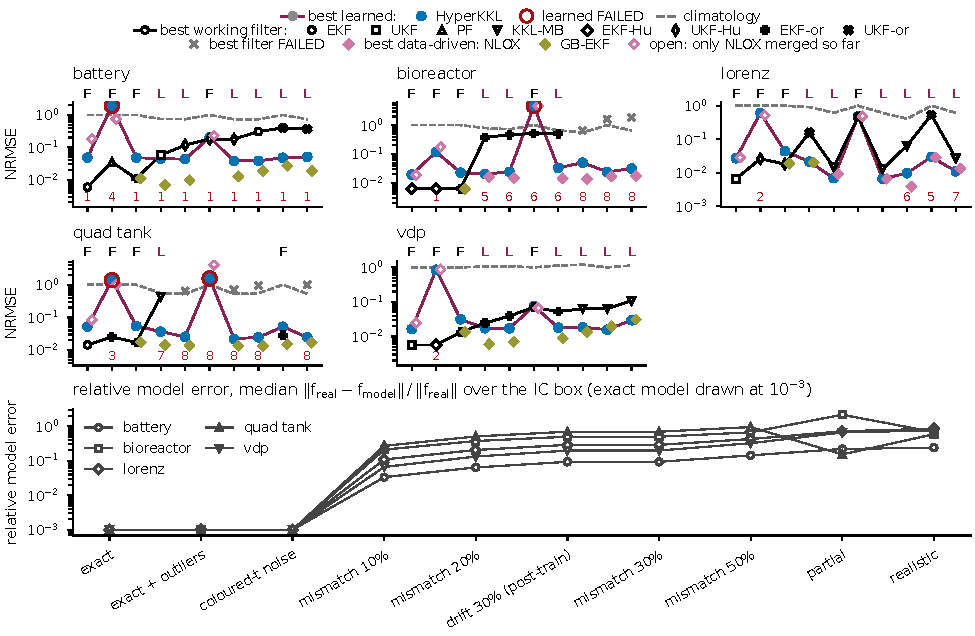
\includegraphics[width=0.85\textwidth]{fig3_c3_crossover_id.pdf}
\caption{As Figure~\ref{fig:c3}, in-distribution tier (\tier{id}). Climatology for \tier{id} is analytic for the nominal plant and a proxy for a perturbed plant (Appendix~\ref{app:protocol}).}
\label{fig:c3id}
\end{figure}

\begin{figure}[p]
\centering
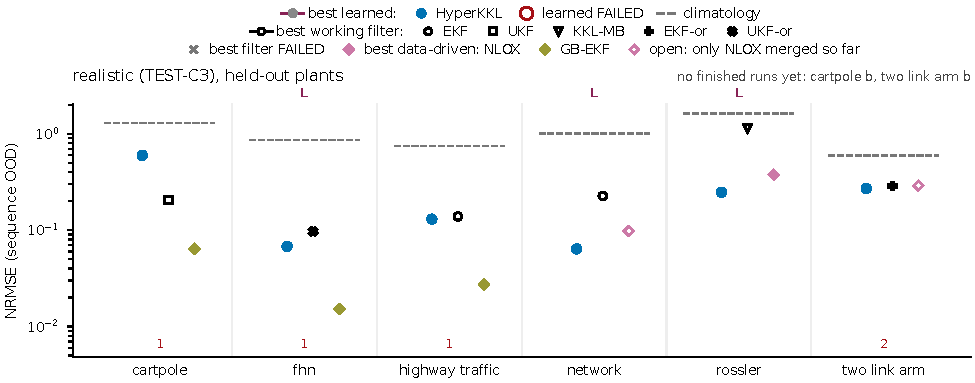
\includegraphics[width=0.85\textwidth]{fig3_c3_crossover_test.pdf}
\caption{As Figure~\ref{fig:c3} for the held-out plants under the realistic deployment (\node{TEST-C3}, frozen recipe, run once): \OutcomeTESTCThree\ at the time of generation (\JobsTESTCThree\ jobs finished); plants without finished runs are marked PENDING.}
\label{fig:c3test}
\end{figure}

\FloatBarrier
\subsection{C2: forgetting floor, memory probe and window sweeps}
\begin{figure}[tbp]
\centering
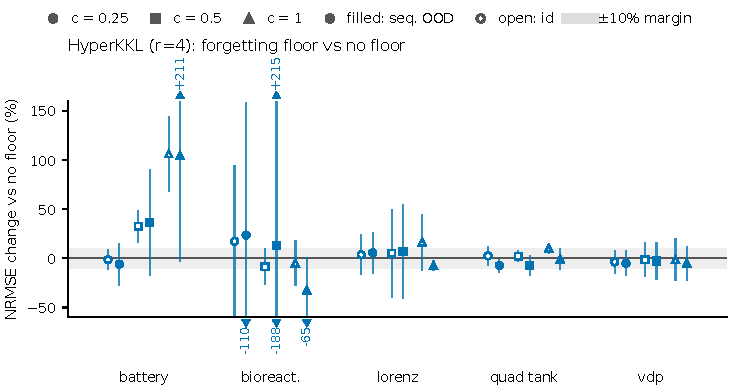
\includegraphics[width=\textwidth]{fig2a_c2_floor.pdf}
\caption{C2 forgetting-floor intervention: change in NRMSE when the SFM context is forced to forget at $\ge c\alpha$, relative to no floor (paired, 3 seeds, 95\% CI; grey band: $\pm10\%$ equivalence margin). The pre-registered rule at $c=0.5$ fails. }
\label{fig:c2floor}
\end{figure}

\begin{figure}[tbp]
\centering
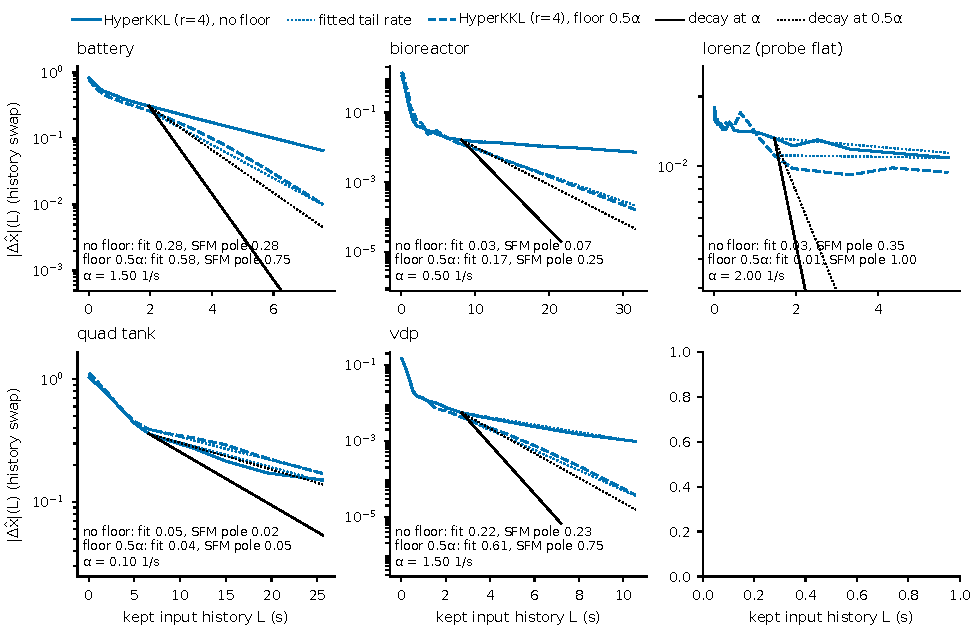
\includegraphics[width=\textwidth]{fig2b_c2_probe.pdf}
\caption{C2 memory probe (\tier{id}, 16 episodes, geometric mean over seeds): decoded change $|\Delta\hat x|$ when the last $L$ seconds of input are kept and everything older is swapped for another episode's input, with and without a $0.5\alpha$ forgetting floor. Black lines: decay at the design rate $\alpha$ (Lemma~\ref{lem:m2-tail}) and at $0.5\alpha$; coloured dotted lines: fitted tail rates. The \sys{lorenz} probe is flat.}
\label{fig:c2probe}
\end{figure}

\begin{figure}[tbp]
\centering
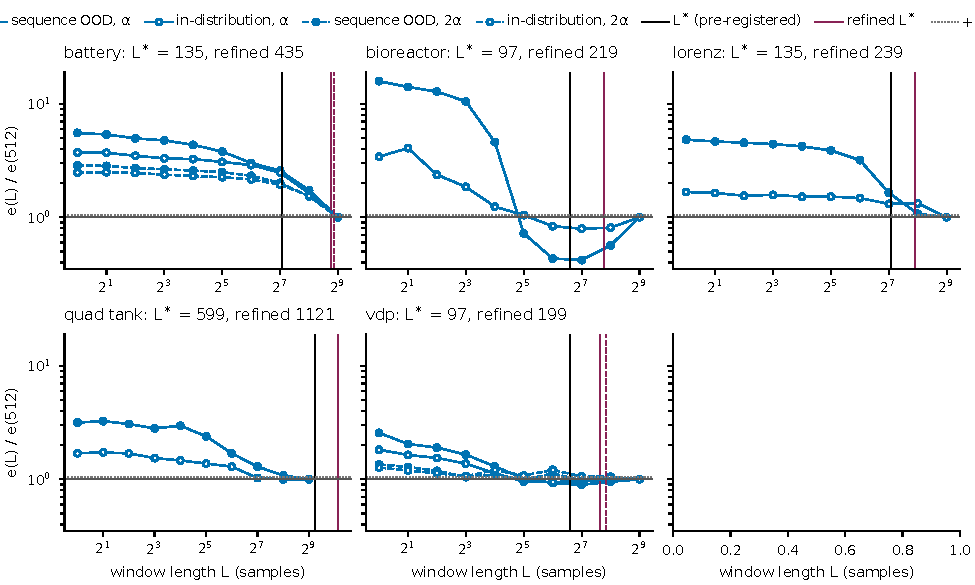
\includegraphics[width=\textwidth]{fig2c_c2_window.pdf}
\caption{C2 window sweeps (HyperKKL $r=4$ with a raw window encoder, mean over 3 seeds): $e(L)/e(512)$ against the window length in samples at the default bandwidth and, on three plants, at $2\alpha$. Black: pre-registered window $L^*=\ln(1/\eta)/\alpha$ ($\eta=0.05$); wine: refined $L^*=(\ln(1/\eta)+\ln\ell)/\alpha$ with the phase-1 proxy for $\ell$ (post hoc). Dotted: $+5\%$.}
\label{fig:c2window}
\end{figure}

\FloatBarrier
\subsection{Deployment scorecard}
\begin{figure}[p]
\centering
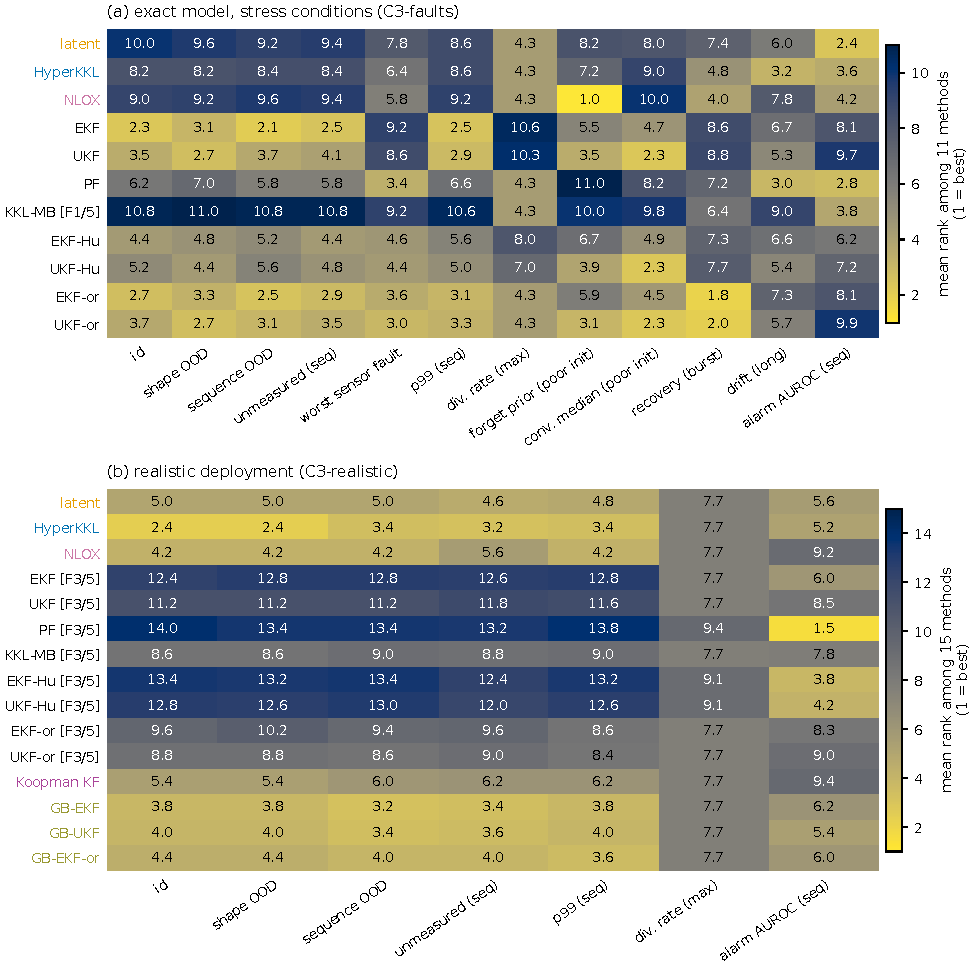
\includegraphics[width=0.95\textwidth]{fig4_scorecard.pdf}
\caption{Deployment scorecard as mean rank per column over the dev plants (1 = best). (a) exact model under the stress conditions of \node{C3-faults}; (b) realistic deployment (\node{C3-realistic}). [F$k$/6]: the method's \tier{sequence\_ood} NRMSE is above climatology on $k$ of six plants.}
\label{fig:scorecard}
\end{figure}
\inputonce{generated/tab3_scorecard_realistic}

\FloatBarrier
\subsection{Every decision rule}
\inputonce{generated/tab4_decisions}

\section{Real-data validation: details}\label{app:realdata}

All numbers here are macros generated by \texttt{analysis/real\_numbers.py} from \texttt{experiments/real/results.json}; the pre-registration is \texttt{experiments/real/DESIGN.md} (written before any training or evaluation) and the data provenance \texttt{DATA.md}.

\paragraph{Data.} Panasonic NCR18650PF cell, Kollmeyer, Mendeley Data v1, DOI 10.17632/wykht8y7tg.1, CC BY 4.0 \citep{kollmeyer2018panasonic}; every downloaded file's SHA-256 matches the repository's. Resampled to $dt=1$\,s; input $u$ = mean current over the second (discharge positive); outputs $y=(\Delta T, V_m)$: case-temperature rise and the terminal voltage behind the plant's 2-s acquisition filter, so that every observer uses the unchanged $y=x[\text{sensors}]$ contract of the simulated battery plant. States $(\mathrm{SOC},V_1,V_2,\Delta T,V_m)$; labelled on real data: SOC (coulomb count), $\Delta T$, $V_m$; $V_1,V_2$ have no labels and are excluded from the phase-2 loss. Split by drive cycle at 25$^\circ$C: train Cycle 1--3, UDDS, LA92; validation Cycle 4; test US06, HWFET (HWFTa and HWFTb pooled), NN; disjoint files and absolute time intervals. Disclosed overlap of shapes: the Cycle 1--4 mixes contain US06/HWFET/NN segments and NN combines US06 and LA92 portions, so the test cycles are new \emph{sequences} on real hardware, not wholly new waveform shapes.

\paragraph{Model identification.} 2-RC equivalent circuit with constant parameters identified by least squares on the training cycles: $R_0=\RealEcmRZero$\,m$\Omega$, $\tau_1=\RealEcmTauOne$\,s, $\tau_2=\RealEcmTauTwo$\,s, $Q=\RealQAh$\,Ah (C/20 capacity), OCV polynomial, lumped thermal model. Open-loop terminal-voltage RMSE \RealVmFitTrainMin--\RealVmFitTrainMax\,mV on the training cycles, \RealVmFitValTestMin--\RealVmFitValTestMax\,mV on validation/test (US06 \RealVmFitUsZeroSix\,mV, errors up to \RealEcmVmax\,V near empty), \RealVmFitZeroMin--\RealVmFitZeroMax\,mV at 0$^\circ$C with Arrhenius-scaled resistances (factor \RealArrheniusFactor): a realistic but incomplete model, as intended.

\paragraph{Observers.} Learned KKL: the paper's default recipe ($n_z=7$, $\alpha=\RealAlpha$/min so that $dt=1$\,s passes the design gate, SFM context, budget 140k (\RealParamsMin--\RealParamsMax\ parameters per conditioner), 3000 phase-2 steps, \RealNSeeds\ seeds). Phase 1 on the identified circuit (zero-input episodes, collocation states, and the training currents replayed on the model); phase 2 is the unchanged \texttt{train.phase2} on real training windows with the loss restricted to the labelled states. WS-best: per seed, whichever of HyperKKL ($r=4$) and its dense-subspace ablation has the lower validation SOC RMSE (\RealWsChoice); the single-method reading uses the $r=4$ rows (HyperKKL vs EKF: \RealLoraEkfCyclesABetter\ of 3 cycles decided for HyperKKL; vs latent: \RealLoraLatentCyclesABetter\ of 3, differences US06 \RealLoraLatentUSZeroSixDiff\ [\RealLoraLatentUSZeroSixCiLo, \RealLoraLatentUSZeroSixCiHi], HWFET \RealLoraLatentHWFETDiff\ [\RealLoraLatentHWFETCiLo, \RealLoraLatentHWFETCiHi], NN \RealLoraLatentNNDiff\ [\RealLoraLatentNNCiLo, \RealLoraLatentNNCiHi]; per-seed means \RealLoraLatentUSZeroSixSeeds; \RealLoraLatentHWFETSeeds; \RealLoraLatentNNSeeds). Filters: the unchanged EKF/UKF on the identified circuit, $Q,R$ from a 72-point grid scored on the validation cycle with the same wrong-prior protocol (oracle-tuned, as \texttt{ekf\_oracle}); the EKF's chosen $r_{V_m}=\RealEkfRvm$\,V sits at the top of the pre-registered grid (score flat there), the UKF's (\RealUkfRvm\,V) is interior. Reference: coulomb counting from the wrong prior (error 20\% by construction). Episodes: 30-min windows every 5\,min through each discharge (US06 \RealNwinUsZeroSix\ windows, HWFET \RealNwinHwfet, NN \RealNwinNn; validation \RealNwinVal), each run with prior $\mathrm{SOC}_0\pm0.2$ where that stays in $[0,1]$.

\paragraph{Statistics and rules.} Per-window paired differences averaged over prior signs and seeds; 95\% moving-block bootstrap over window start times (block 30\,min, 10\,000 resamples) and per-seed means; a cycle counts only if the CI excludes 0 \emph{and} all seeds agree. H1: WS-best beats the tuned EKF on $\ge2$ of 3 test cycles; H2: WS-best beats latent injection, same rule. Everything else is descriptive.

% generated by analysis/real_numbers.py -- do not edit by hand
\begin{table}[t]
\centering\small
\setlength{\tabcolsep}{5pt}
\caption{Real-data validation: settled SOC RMSE [\% SOC] ($t\ge15$ min of 30-min windows, prior SOC 20\% off) on the three held-out 25$^\circ$C drive cycles and on the validation cycle (Cycle 4, used for model selection and filter tuning only). Learned: mean $\pm$ sd over 3 seeds. WS-best = HyperKKL ($r=4$) or its dense-subspace ablation, whichever has the lower validation RMSE per seed (the pre-registered selection). Same-data baselines (Koopman KF, grey-box EKF/UKF): pending.}
\label{tab:real}
\begin{tabular}{@{}lrrrr@{}}
\toprule
method & US06 & HWFET & NN & validation \\
\midrule
WS-best (HyperKKL $r=4$ or dense ablation, chosen per seed on validation) & \textbf{1.76 $\pm$ 0.15} & \textbf{0.86 $\pm$ 0.05} & \textbf{0.69 $\pm$ 0.04} & 0.71 \\
HyperKKL ($r=4$) & 2.18 $\pm$ 0.59 & 0.91 $\pm$ 0.11 & 0.73 $\pm$ 0.04 & 0.75 \\
dense-subspace ablation & 1.75 $\pm$ 0.25 & 0.93 $\pm$ 0.08 & 0.69 $\pm$ 0.03 & 0.77 \\
latent injection & 2.44 $\pm$ 0.58 & 1.09 $\pm$ 0.10 & 1.25 $\pm$ 0.22 & 1.34 \\
concat (additive) & 7.37 $\pm$ 1.22 & 2.80 $\pm$ 0.14 & 4.51 $\pm$ 0.11 & 4.11 \\
autonomous (no input) & 31.52 $\pm$ 2.65 & 15.54 $\pm$ 0.60 & 31.08 $\pm$ 1.55 & 23.07 \\
EKF (identified 2-RC ECM, $Q,R$ tuned on validation) & 8.85 & 1.19 & 1.95 & 3.25 \\
UKF (same model, tuned) & 9.13 & 1.39 & 1.55 & 3.10 \\
coulomb counting from the wrong prior & 20.00 & 20.00 & 20.00 & 20.00 \\
hyperkkl & 2.18 $\pm$ 0.59 & 0.91 $\pm$ 0.11 & 0.73 $\pm$ 0.04 & 0.75 \\
\bottomrule
\end{tabular}
\end{table}


\paragraph{Results.} H1: learned better on \RealHOneLearnedBetter, EKF better on \RealHOneEkfBetter\ of \RealNTestCycles\ cycles. Paired settled-RMSE differences (WS-best $-$ EKF, \% SOC; CI; per-seed means): US06 \RealWsBestEkfUSZeroSixDiff\ [\RealWsBestEkfUSZeroSixCiLo, \RealWsBestEkfUSZeroSixCiHi] (\RealWsBestEkfUSZeroSixSeeds); HWFET \RealWsBestEkfHWFETDiff\ [\RealWsBestEkfHWFETCiLo, \RealWsBestEkfHWFETCiHi] (\RealWsBestEkfHWFETSeeds); NN \RealWsBestEkfNNDiff\ [\RealWsBestEkfNNCiLo, \RealWsBestEkfNNCiHi] (\RealWsBestEkfNNSeeds). Against the UKF: US06 \RealWsBestUkfUSZeroSixDiff, HWFET \RealWsBestUkfHWFETDiff, NN \RealWsBestUkfNNDiff\ (all CIs below 0, all seeds negative). H2: weight-space better on \RealHTwoWsBetter, latent better on \RealHTwoLatentBetter: US06 \RealWsBestLatentUSZeroSixDiff\ [\RealWsBestLatentUSZeroSixCiLo, \RealWsBestLatentUSZeroSixCiHi] (\RealWsBestLatentUSZeroSixSeeds); HWFET \RealWsBestLatentHWFETDiff\ [\RealWsBestLatentHWFETCiLo, \RealWsBestLatentHWFETCiHi] (\RealWsBestLatentHWFETSeeds); NN \RealWsBestLatentNNDiff\ [\RealWsBestLatentNNCiLo, \RealWsBestLatentNNCiHi] (\RealWsBestLatentNNSeeds). Maximum settled error: US06 WS-best \RealWsBestUSZeroSixMax\,\% vs EKF \RealEkfUSZeroSixMax\,\%; HWFET \RealWsBestHWFETMax\ vs \RealEkfHWFETMax; NN \RealWsBestNNMax\ vs \RealEkfNNMax. Median time to stay within 5\% SOC (30-min windows): WS-best US06 \RealWsBestUSZeroSixTconv\,min, HWFET \RealWsBestHWFETTconv, NN \RealWsBestNNTconv; EKF \RealEkfUSZeroSixTconv\ (never within 5\% on US06 windows), \RealEkfHWFETTconv, \RealEkfNNTconv. The learned estimate has a sample-level ripple of 1--2\% SOC (Figure~\ref{fig:real}); no output smoothing was applied to any method.

\begin{figure}[t]
\centering
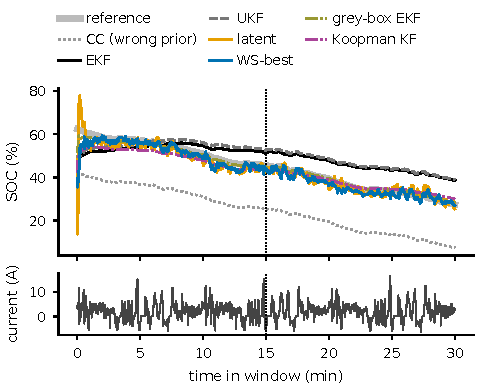
\includegraphics[width=0.49\textwidth]{us06_window.pdf}\hfill
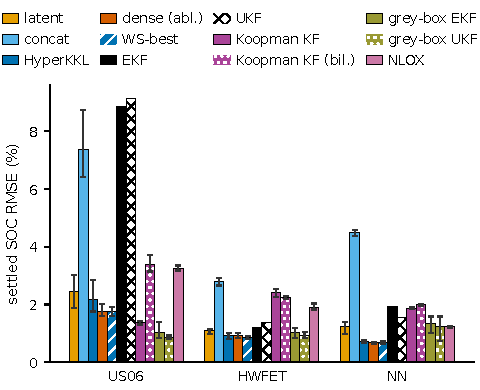
\includegraphics[width=0.49\textwidth]{rmse_test25.pdf}
\caption{Real data, 25$^\circ$C. Left: one US06 window from a prior 20\% off (the EKF settles on a biased SOC; the learned observer corrects it from data with a visible ripple). Dotted line: start of the settled window ($t\ge15$\,min); the current is positive on discharge. Right: settled SOC RMSE per method and test cycle, prior SOC $\pm20\%$; learned observers: mean over 3 seeds, whiskers min--max (\texttt{experiments/real/figures/}).}
\label{fig:real}
\end{figure}

\paragraph{Whole discharges (secondary).} From full charge with prior SOC 0.8, RMSE over $t\ge15$\,min: US06 WS-best \RealWholeWsBestUSZeroSix\ vs EKF \RealWholeEkfUSZeroSix\ / UKF \RealWholeUkfUSZeroSix; HWFTa \RealWholeWsBestHWFTa\ vs \RealWholeEkfHWFTa\ / \RealWholeUkfHWFTa; HWFTb \RealWholeWsBestHWFTb\ vs \RealWholeEkfHWFTb\ / \RealWholeUkfHWFTb; NN \RealWholeWsBestNN\ vs \RealWholeEkfNN\ / \RealWholeUkfNN. With hours to converge the filters match the learned observers on the mild cycles; the advantage on those cycles is convergence speed from a wrong prior, and on the aggressive cycle it is accuracy.

\paragraph{Temperature shift (secondary, 0$^\circ$C).} Models trained and identified at 25$^\circ$C only, evaluated on every 0$^\circ$C drive cycle. The claim does \emph{not} transfer: the EKF (Arrhenius-scaled resistances) is better on \RealZeroEkfBetter\ of \RealZeroNCycles\ cycles (learned \RealZeroWsRmseMin--\RealZeroWsRmseMax\,\%, EKF \RealZeroEkfRmseMin--\RealZeroEkfRmseMax\,\%); the learned observers win only on \RealZeroWsBetterCycles. The decoder has never seen the 0$^\circ$C voltage--SOC--current relationship, whereas the filter carries an explicit temperature model. Weight-space vs latent is decided for neither side on \RealZeroWsLatentTies\ of \RealZeroNCycles\ cycles. Training on several temperatures (the dataset covers $-20$ to 25$^\circ$C) is the obvious next step and was not part of the pre-registration.

\paragraph{Limitations (as recorded in the experiment report).} (1) The reference SOC is coulomb counting, the standard in this literature but itself an estimate (tester current error; capacity measured once at C/20 after the drive cycles, i.e.\ after some ageing; SOC $=1$ at the end of each CC--CV charge by definition); using the nominal 2.9\,Ah instead would shift the reference by up to 2.8\% SOC at the end of a discharge; the learned methods are trained on this reference and can absorb its convention. (2) One cell, one test campaign: windows within a cycle are dependent (handled by the block bootstrap), cell-to-cell variation is not sampled, and US06 has only \RealNwinUsZeroSix\ windows. (3) The advantage holds at the training temperature only. (4) The filters use a constant-parameter 2-RC circuit without hysteresis or SOC-dependent resistance, i.e.\ what a quick least-squares identification gives; a richer model (lookup tables from the HPPC tests, a hysteresis state) would narrow the gap and was not built. This is the incomplete-model regime of C3 by design. (5) The short-window protocol favours fast convergence. (6) The learned estimate has sample-level ripple. Deviations from the pre-registration (implementation only): filters run batched on GPU over the whole $Q,R$ grid (tested equal to individual filters); phase-1 simulations use clean outputs and no process noise; not run: the strict shape split, the residual alarm, NLOX, and the same-data baselines (\RealSameDataBaselines).

\section{History of the study: what was tried, superseded or abandoned}\label{app:history}

This appendix is the part of the record that a reader needs to judge how much freedom the authors had. It is condensed from the generated history of the experiment tree (\texttt{experiments/HISTORY.md}, built from the node files, the journal and the mechanical verdicts).

\paragraph{Protocol v1 (archived).} A first tree used an \emph{amplitude} OOD tier (inputs scaled beyond the training range) next to a waveform tier, five dev plants and nominal filters only. Its single-winner C1 rule also failed mechanically (preferred location: none, at the $\ge4/5$ bar), its exact-model C3 rule failed (filters won on every plant), and its mismatch nodes gave mixed verdicts at 10--20\% and passes at 30--50\%. The protocol was archived because the amplitude tier drove inputs beyond the physical input bounds of bounded plants (the bioreactor's dilution rate, the traffic ramp), so that ``OOD'' amplitudes were compressed by the actuator and the tier did not test what it claimed. Protocol v2 replaced it by the shape and sequence tiers inside one amplitude box, per-plant $t_\mathrm{ref}$, partial-knowledge models, coloured Student-$t$ noise, robust and oracle filters, the deployment scorecard and a sixth dev plant (\sys{battery}). Every v2 node was re-registered with its rule before its runs; no v1 number appears in this paper.

\paragraph{Dead ends.} A 5\% mismatch node failed most of its jobs twice in v1 and was dropped (the v2 sweep starts at 10\%, which is why the crossover below 10\% is not located). A control that trained the latent variant with a one-step rollout failed jobs twice and was not carried to v2; the latent variant's trainability confound (Section~\ref{sec:c1}) is therefore unresolved. Two v1 bugs in the plant-perturbation rule (the bioreactor's operating point and the quad-tank's gravity and valve constants were scaled with the ``physical parameters'', rejecting every episode) were fixed before v2 and the affected runs moved out of the tree.

\paragraph{Verbal readings corrected by the mechanical verdicts.} Before the results layer existed, interim digests read the forgetting-floor node as ``passes on 5/6'' and the partial-model-helps comparison as ``8$\times$ worse without the model on the bioreactor''; the mechanical application of the rules gives \OutcomeCTwoFloorFive\ (no-loss \CtwoFloorFiveNoLoss, TOST \CtwoFloorFiveTostNonInferior, probe \CtwoFloorFiveProbeAboveFloor) and \OutcomeCThreePartialModelfree\ (the bioreactor difference is not significant at three seeds). The digest's attribution of the battery's memory need to the theory's lower bound was withdrawn in the theory revision; the sufficient-side explanation through $\ln\ell$ replaced it (Corollary~\ref{cor:m2-rule}). The C1 rank controls were expected to pass and \FAIL.

\paragraph{Data problems recorded by the results layer.} \node{TEST-C1}'s eighteen runs come from four snapshots of the code (per plant: \sys{network} from one, \sys{cartpole}, \sys{fhn} (two seeds) and \sys{highway\_traffic} from a second, \sys{fhn} (third seed) and \sys{two\_link\_arm} from a third, \sys{rossler} from a fourth); \node{C1-budget-s}'s runs come from two snapshots; the node files and recipes were frozen throughout, and the verdicts are reported as the layer prints them. The same-data comparison (b) was added after the simulated reviews and is labelled not pre-registered wherever it appears. The decisions table overflows its width by up to 4\,pt.

\paragraph{Pending at the time of writing.} \node{C1-modelfree} (\OutcomeCOneModelfree), the learning-curve nodes \node{C3-data50} and \node{C3-data150} (\OutcomeCThreeDataFifty, \OutcomeCThreeDataOneFiveZero), the base-width controls (\OutcomeCOneBasewidthSixtyFour, \OutcomeCOneBasewidthTwoFiveSix), the third seeds of the budget controls (\JobsCOneBudgetS, \JobsCOneBudgetL\ jobs finished), and \node{TEST-C3} (\OutcomeTESTCThree, \JobsTESTCThree). The Koopman Kalman filter and grey-box EKF baselines and the real-data battery experiment are implemented and pre-registered and are not part of this version.

\paragraph{Simulated reviews.} Five simulated reviews written from the perspective of likely action editors (control theory, Koopman methods, dynamical-systems reconstruction, deep learning for dynamics, ML theory) were commissioned on the theory and the interim results before this draft; their must-fix items (a circular contraction hypothesis, a hidden reachability hypothesis in the window lower bound, the chaotic-plant caveats, the missing model-incompleteness proposition, the single-winner C1 rule, the capacity description of the hypernetwork, the climatology reference, the label requirement, the same-data baselines) are addressed in the theory revision and in the framing of this paper, or listed above as open.


\end{document}
